%\documentclass[a4paper,12pt,oneside,openright,nohints]{report}
\documentclass[a4paper,12pt,twoside,openright,nohints]{report} % to print (also, remember to change headers)

% ~~~~~~~~~~~~~~~~~~~~

% Preamble structure files
% CORE MODULES
% ~~~~~~~~~~~~
% Standard package for selecting font encodings
% https://ctan.org/pkg/fontenc
\usepackage[T1]{fontenc}

% Language support
% https://ctan.org/pkg/babel
\usepackage[UKenglish]{babel}

% Enhanced support for graphics
% https://ctan.org/pkg/graphicx
\usepackage{graphicx}

% Driver-independent colour extensions
% https://ctan.org/pkg/xcolor
\usepackage[dvipsnames]{xcolor}



% PAGE FORMATTING
% ~~~~~~~~~~~~~~~
% Flexible and complete interface to document dimensions
% https://ctan.org/pkg/geometry
\usepackage[lmargin=3.0cm,rmargin=2.3cm]{geometry}

% Draw a page-layout diagram
% https://ctan.org/pkg/showframe
%\usepackage{showframe}
%\renewcommand*\ShowFrameColor{\color{red!10}}

% Intermix single and multiple columns
% https://ctan.org/pkg/multicol
\usepackage{multicol}

% Set space between lines
% https://ctan.org/pkg/setspace
\usepackage{setspace}

% Control page headers and footers
% https://ctan.org/pkg/fancyhdr
\usepackage{fancyhdr}

% Improve footnote handling
% https://ctan.org/pkg/footnote
%\usepackage{footnote}

% A range of footnote options
% https://ctan.org/pkg/footmisc
\usepackage[perpage]{footmisc}

% Select alternative section titles
% https://ctan.org/pkg/titlesec
%\usepackage{titlesec,titletoc}

% Add epigraphs (quotes at the start of chapters)
% https://ctan.org/pkg/epigraph
\usepackage{epigraph}

% Insert whole PDF documents with the \includepdf command
% https://ctan.org/pkg/pdfpages
\usepackage{pdfpages}

% Make a page landscape orientated
% https://ctan.org/pkg/pdflscape
\usepackage{pdflscape}

% Execute command after the next page break
% https://ctan.org/pkg/afterpage
\usepackage{afterpage}



% TEXT FORMATTING
% ~~~~~~~~~~~~~~~
% Format headers (e.g. \sectionfont)
% https://ctan.org/pkg/sectsty
\usepackage{sectsty}

% Format hyperlinks (\href, \url)
% https://ctan.org/pkg/hyperref
\usepackage[pdfusetitle,      % Gets PDF metadata from \author and \title
			breaklinks=true,  % Allow links to break over lines
			colorlinks=true,  % Colours links instead of the default boxes
			linkcolor=black,  % Colour of internal links
			urlcolor=blue,    % Colour of external hyperlinks
			citecolor=blue,   % Colour of citations
			]{hyperref}

% Make reference to section names, etc
% https://ctan.org/pkg/nameref
\usepackage{nameref}

% Context sensitive quotation facilities
% https://ctan.org/pkg/csquotes
\usepackage{csquotes}



% TITLE PAGE
% ~~~~~~~~~~~~
% Control over the typesetting of the \maketitle command
% https://ctan.org/pkg/titling
\usepackage{titling}



% GLOSSARY
% ~~~~~~~~
% Create glossaries and lists of acronyms
% https://ctan.org/pkg/glossaries
\usepackage[acronym,shortcuts]{glossaries}

% Control of acronyms
% https://ctan.org/pkg/acronym
%\usepackage[printonlyused,nohyperlinks]{acronym}




% BIBLIOGRAPHY
% ~~~~~~~~~~~~
% Flexible bibliography support
% https://ctan.org/pkg/natbib
%\usepackage{natbib}

% Sophisticated Bibliographies
% https://ctan.org/pkg/biblatex
\usepackage[backend=bibtex,      % Specifies the database backend
			bibencoding=ascii,   % Bibtex backend expects ASCII
			style=authoryear,    % Style
			natbib=true,         % Aliases for natbib commands (\cite, \citep etc)
			dashed=false,        % No dashes for the same author
%			maxnames=2,          % Limit number of authors printed
%			minnames=1,          % Limit number of authors printed
			url=false,           % Controls whether URLs are printed
			doi=false,           % Controls whether DOIs are printed
			isbn=false,          % Controls whether ISBNs are printed
			eprint=false,        % Controls whether ArXiv details are printed
%			sortcites=true,
			uniquename=init,
			giveninits=true,
			sorting=nyvt,
			]{biblatex}



% APPENDIX
%~~~~~~~~~
% Extra control of appendices
% https://ctan.org/pkg/appendix
\usepackage[titletoc]{appendix}



% FLOATS
% ~~~~~~
% Improved interface for floating objects (figures, tables etc)
% https://ctan.org/pkg/float
\usepackage{float}

% Customising captions in floating environments
% https://ctan.org/pkg/caption
%\usepackage{caption}

% Retain float number across several floats
% https://ctan.org/pkg/captcont
\usepackage{captcont}

% Control float placement
% https://ctan.org/pkg/placeins
\usepackage[section]{placeins}

% Rotation tools, including rotated full-page floats
% https://ctan.org/pkg/rotating
\usepackage{rotating}

% Rotate floats, i.e. combining the rotating and float packages
% https://ctan.org/pkg/rotfloat
\usepackage{rotfloat}



% FIGURES
% ~~~~~~~
% Produces figures which text can flow around
% https://ctan.org/pkg/wrapfig
\usepackage{wrapfig}

% Convert EPS to PDF, so you can include .eps figures with pdflatex
% https://ctan.org/pkg/epstopdf
% \usepackage{epstopdf}



% TABLES
% ~~~~~~~
% Publication quality tables in LaTeX
% https://ctan.org/pkg/booktabs
\usepackage{booktabs}

% Allow tables to flow over page boundaries
% https://ctan.org/pkg/longtable
\usepackage{longtable}

% Create tabular cells spanning multiple rows
% https://ctan.org/pkg/multirow
\usepackage{multirow}

% Tabular column heads and multi-lined cells
% https://ctan.org/pkg/makecell
\usepackage{makecell}



% CONTENTS
% ~~~~~~~~
% Produce a table of contents for each chapter, part or section
% https://ctan.org/pkg/minitoc
\usepackage{minitoc}



% SCIENTIFIC
% ~~~~~~~~~~
% AMS mathematical facilities
% https://ctan.org/pkg/amsmath
\usepackage{amsmath,amssymb,amsthm}

% Macros for AAS Journals, includes journals (\mnras)
% https://ctan.org/pkg/aastex
\usepackage{aas_macros}

% Comprehensive SI units and number formatting, use \SI{9.81}{\meter\per\second\squared}
% https://ctan.org/pkg/siunitx
\usepackage{siunitx}

% Typeset in-line fractions in a "nice" way
% https://ctan.org/pkg/nicefrac
\usepackage{nicefrac}

% Typeset source code listings
% https://ctan.org/pkg/listings
\usepackage{listings}



% SYMBOLS
% ~~~~~~~
% Access to PostScript standard Symbol and Dingbats fonts
% https://ctan.org/pkg/pifont
\usepackage{pifont}

% St Mary Road symbols for theoretical computer science
% https://ctan.org/pkg/stmaryrd
\usepackage{stmaryrd}

% Martin Vogel's Symbols (contains astronomical/astrological icons)
% https://ctan.org/pkg/marvosym
\usepackage{marvosym}




% MISCELLANEOUS
% ~~~~~~~~~~~~~
% Add \verbatim and \comment environments
% https://ctan.org/pkg/verbatim
\usepackage{verbatim}

% Formats for dates, times and time zones
% https://ctan.org/pkg/datetime2
\usepackage{datetime2}

% Easy access to the Lorem Ipsum dummy text (\lipsum)
% https://ctan.org/pkg/lipsum
\usepackage{lipsum}

% Mark things to do
% https://ctan.org/pkg/todonotes
\usepackage[colorinlistoftodos]{todonotes}

% Extended conditional commands
% https://ctan.org/pkg/xifthen
\usepackage{xifthen}

% icons
\newcommand{\tick}{\ding{52}}
\newcommand{\uptriangle}{\ding{115}}
\newcommand{\backarrow}{\rotatebox[origin=c]{180}{\ding{252}}}
\newcommand{\blackdiamond}{\ding{117}}
\newcommand{\about}{\ensuremath{\sim}}
\newcommand{\done}{\textcolor{green}{~\tick~}}

% superscript
\newcommand{\st}{\ensuremath{^{\rm st}}}
\newcommand{\nd}{\ensuremath{^{\rm nd}}}
\newcommand{\rd}{\ensuremath{^{\rm rd}}}
\newcommand{\nth}{\ensuremath{^{\rm th}}}

% code (see JSS style - https://www.jstatsoft.org/pages/view/style)
% programs (Word, IRAF, VSCode...)
%\newcommand{\software}{\textsc}
\newcommand{\software}{\textsf}
% names of programming languages (C, Python...)
\newcommand{\proglang}{\textsf}
% names of packages (astropy, matplotlib...)
%\newcommand{\pkg}[1]{{\fontseries{b}\selectfont #1}}
\newcommand{\pkg}{\texttt}
% inline code
\newcommand{\code}{\texttt}

% coloured text
\newcommand{\rtxt}[1]{\textcolor{red}{#1}}


% insert a blank page
\newcommand\blankpage{
    \null{}
    \thispagestyle{empty}
    \addtocounter{page}{-1}
    \newpage
    }

% a completely blank environment, so I can collapse sections nicely
\newenvironment{colsection}{}{}

% format a quote
\newcommand\makequote[3]{
    \begin{center}
        \Huge{\textbf{\textcolor{GOTOlightblue}{``~~}}}\\
            \LARGE{#1}\\
        \vspace{0.3cm}
        \Huge{\textbf{\textcolor{GOTOlightblue}{~~''}}}
    \end{center}
    \vspace{-0.7cm} \hspace{8cm}
    \large{ --- #2\ifthenelse{\isempty{#3}}{}{, \textit{#3}}}
    }

% resize ToC numbers to fit in >100
% https://tex.stackexchange.com/questions/49887/
\makeatletter
\renewcommand{\@pnumwidth}{3em}
\renewcommand{\@tocrmarg}{4em}
\makeatother

% add a small contents to the start of a chapter
\mtcsettitle{minitoc}{}
\mtcsetrules{*}{off}
\mtcsetfont{minitoc}{section}{\normalsize\bfseries}
\mtcsetfont{minitoc}{subsection}{\normalsize}
\mtcsetoffset{minitoc}{-1em}
\setlength{\mtcindent}{-0.9em}
\let\oldappendices\appendices\def\appendices{\oldappendices\adjustmtc}
\newcommand\chaptoc{
    \begin{singlespacing}
    \vspace{-1.4cm}
    \noindent{\color{GOTOlightblue}\rule{\textwidth}{1.5pt}}
    \vspace{-0.7cm}
    {\hypersetup{linkcolor=black}
    \minitoc{}
    }
    \vspace{-0.2cm}
    \noindent{\color{GOTOlightblue}\rule{\textwidth}{1.5pt}}
    \begin{center}
        \hyperref[contents]{\textcolor{white}{\uptriangle}}
    \end{center}
    \end{singlespacing}
    }

% reference functions containing the type, also name
\AtBeginDocument{%
    \renewcommand\chapterautorefname{Chapter}%
    \renewcommand\sectionautorefname{Section}%
    \renewcommand\subsectionautorefname{Section}%
}
\newcommand\aref[1]{\autoref{#1}}
\newcommand\nref[1]{\autoref{#1} (\nameref{#1})}

% Cite functions linking the name as well as the year
% https://tex.stackexchange.com/questions/15951/hyperlink-name-with-biblatex-authoryear-biblatex-1-4b
\DeclareFieldFormat{citehyperref}{%
  \DeclareFieldAlias{bibhyperref}{noformat}% Avoid nested links
  \bibhyperref{#1}}
\DeclareFieldFormat{textcitehyperref}{%
  \DeclareFieldAlias{bibhyperref}{noformat}% Avoid nested links
  \bibhyperref{%
    #1%
    \ifbool{cbx:parens}
      {\bibcloseparen\global\boolfalse{cbx:parens}}
      {}}}
\savebibmacro{cite}
\savebibmacro{textcite}
\renewbibmacro*{cite}{%
  \printtext[citehyperref]{%
    \restorebibmacro{cite}%
    \usebibmacro{cite}}}
\renewbibmacro*{textcite}{%
  \ifboolexpr{
    (not test {\iffieldundef{prenote}} and
      test {\ifnumequal{\value{citecount}}{1}})
    or
    (not test {\iffieldundef{postnote}} and
      test {\ifnumequal{\value{citecount}}{\value{citetotal}}})
  }
    {\DeclareFieldAlias{textcitehyperref}{noformat}}
    {}%
  \printtext[textcitehyperref]{%
    \restorebibmacro{textcite}%
    \usebibmacro{textcite}}}

% Remove comma inline citations
\renewcommand*{\nameyeardelim}{\addspace}

% bibliography
\addbibresource{bibliography.bib}
\renewbibmacro{in:}{}
\AtEveryBibitem{\clearfield{title}}
\AtEveryBibitem{\clearfield{pages}}

% margins
\setlength{\marginparwidth}{50pt}
\setlength{\marginparsep}{10pt}
\setlength{\marginparpush}{5pt}

\setlength{\topmargin}{5pt}
\setlength{\headheight}{15pt}
\setlength{\headsep}{25pt}

\setlength{\footskip}{30pt}

\setlength{\textwidth}{\paperwidth}
\addtolength{\textwidth}{-\marginparsep}
\addtolength{\textwidth}{-\oddsidemargin}
\addtolength{\textwidth}{-\marginparwidth}
\addtolength{\textwidth}{-1in}
\addtolength{\textwidth}{-1mm}
\addtolength{\textwidth}{-\hoffset}

\setlength{\textheight}{\paperheight}
\addtolength{\textheight}{-\topmargin}
\addtolength{\textheight}{-\headheight}
\addtolength{\textheight}{-\headsep}
\addtolength{\textheight}{-\footskip}
\addtolength{\textheight}{-1in}
\addtolength{\textheight}{-\voffset}
\addtolength{\textheight}{-2cm}

\setlength{\columnsep}{10pt}
\setlength{\columnseprule}{0pt}
\setlength{\LTcapwidth}{8in}

% headings
\chapterfont{\color{GOTOdarkblue}}
\sectionfont{\color{GOTOdarkblue}}
\subsectionfont{\color{GOTOdarkblue}}
\subsubsectionfont{\color{GOTOdarkblue}}

% header/footer
\pagestyle{fancy}
\renewcommand{\chaptermark}[1]{\markboth{#1}{}}
\renewcommand{\sectionmark}[1]{\markright{#1}}

% one page formatting
\fancyhead[L]{\chaptername\ \thechapter: \leftmark}
\fancyhead[R]{\textbf{\thepage}}

% two page formatting
%\fancyhead[RE]{\chaptername\ \thechapter: \leftmark}
%\fancyhead[LO]{Section \thesection: \rightmark}
%\fancyhead[LE, RO]{\textbf{\thepage}}

\fancyfoot{}

% a good blue for titles
\definecolor{sections}{RGB}{46, 116, 181}

% units for astronomy using the siunitx package
% e.g. \SI{100}{\solarmass\per\second}
\DeclareSIUnit\parsec{pc}
\DeclareSIUnit\lightyear{ly}
\DeclareSIUnit\erg{erg}
\DeclareSIUnit\solarmass{\ensuremath{\textup{M}_\odot}}
\DeclareSIUnit\solarlum{\ensuremath{\textup{L}_\odot}}
\DeclareSIUnit\solarrad{\ensuremath{\textup{R}_\odot}}

\makeglossaries{}

\newacronym{goto}{GOTO}{Gravitational-wave Optical Transient Observer}
\newacronym{fov}{FoV}{Field of View}
\newacronym{gw}{GW}{Gravitational Wave}


% ~~~~~~~~~~~~~~~~~~~~

\begin{document}

% Document properties
\title{A telescope control and scheduling system for the Gravitational-wave Optical Transient Observer}
\author{Martin J Dyer}

% Front pages
\singlespacing{}
\pagenumbering{roman}
\pagestyle{empty}
% ---------
\begin{center}
    
\includegraphics[width=0.45\linewidth]{./images/UoS_logo.pdf}
    
\includegraphics[width=0.45\linewidth]{./images/GOTO_logo.pdf}

    \vspace*{2.5cm}

    % Title
    \begin{Huge}
        \textbf{A telescope control and
               scheduling system for the
               Gravitational-wave Optical Transient Observer
               }
    \end{Huge}

    \vspace*{2.5cm}

    % Author
    \begin{LARGE}
        \text{Martin J. Dyer}
    \end{LARGE}

    \vspace*{1cm}

    % Institute
    \begin{Large}
        Department of Physics and Astronomy \\
        \smallskip
        The University of Sheffield
    \end{Large}

    %\vspace*{2cm}

    % Logo / Coat of Arms
    %
\includegraphics[width=0.4\linewidth]{./images/University_of_Sheffield_logo.png}
    %
\includegraphics[width=0.3\linewidth]{./images/University_of_Sheffield_coat_of_arms.png}

    \vspace*{2.5cm}

    % Purpose
    \begin{large}
        \textit{A dissertation submitted in candidature for the degree of} \\
        \textit{Doctor of Philosophy at the University of Sheffield}
    \end{large}

    \vspace*{1cm}

    % Date
    \begin{large}
        \text{26th September 2019}
        %\text{\today}
    \end{large}

    \vfill
\end{center}

%\makequote{There's no sense crying over every mistake. \\ You just keep on trying `till you run out of cake.}{GLaDOS}{Portal}

%\makequote{Let's all stay positive and do some Science.}{Cave Johnson}{Portal 2}

%\makequote{Think of a quote to put here.}{Joe Bloggs}{The Life of Bloggs}

\vspace{10cm}

\makequote{
%For everyone, as I think, must see that \\
Astronomy compels the soul to look upwards \\
and leads us from this world to another.
}{Plato}{The Republic Book VII, 380 BC}

\vspace{2cm}

\makequote{
Astronomy's much more fun when \\
you're not an astronomer. %\\
%When I was an astronomer most of the time was spent \\
%making equipment, or making it work, or setting it up, \\
%or else typing away at computers to try to analyse the situation. \\
%The amount of time you spend actually looking at what you're doing is very small.
}{Brian May}{Vox interview, 1991 AD}


% Front matter
\doublespacing{}
\pagestyle{plain}
% ---------
\chapter*{Declaration}

\begin{onehalfspace}

\noindent I declare that, unless otherwise stated, the work presented in this thesis is my own.

\bigskip

\noindent No part of this thesis has been accepted or is currently being submitted for any other qualification at the University of Sheffield or elsewhere.

\bigskip

\noindent Some of my work on the GOTO Telescope Control System has previously been published as \citet{Dyer}. This paper forms the basis of Chapters 3, 4 and 5 of this thesis. The other chapters have not been published previously, although the work within them will contribute to future publications.

\end{onehalfspace}

\chapter*{Acknowledgements}

\begin{onehalfspace}

This is the very last thing I'm writing before sending this to print, because I'm awful at writing these sort of things and I kept putting it off. Not that it really matters, of the very few people who will ever read this thesis I'm guessing most will skip over this bit. I always do.

\medskip

Anyway, I'll start by thanking my PhD supervisor Vik Dhillon, for being a fantastic supervisor and mentor over the past four years, as well as, when needed, a 5-star tour guide of La Palma. Thanks also to my second supervisor Ed Daw, whose Physical Computing class I enjoyed both teaching and learning from, as well as Stu, Dave, Steven, Liam, James, Lydia, Pablo and others in the group in Sheffield. I'd also like to thank members of the GOTO collaboration: Danny, Krzysztof, Paul, Joe, James and Ryan at Warwick; Duncan, Kendall, Evert, Travis and Alex at Monash; Gav, Mark and everyone else from the ever-increasing list of member institutions (especially the poor students who had to babysit GOTO for so long). Also my masters project supervisors at Durham, Richard and Tim, who first put me in touch with Vik --- without them I literally would not be where I am today.

\medskip

I'd like to thank all the various friends I've made over the years from Maidenhead, Borlase, Durham and Sheffield; including, but not at all limited to, Alex, Anna, Becky, Ben, Emma, Gemma, Harriet, Harry, Héloïse, James, Katie, Katherine, Laura, Mac, Oliver, Richard, Robin, Simon, Sophie and Varun (I wanted to include as many people as I could, apologies to anyone I forgot). A particular massive thanks to the other PhD students in my year at Sheffield: Becky, Héloïse and Katie. You were the best office-mates and compatriots I could have asked for, and while you all finished before me and went off to better things, it did mean I my own office in the final few weeks --- thanks!

\medskip

Of course, I must also thank my Mum and Dad, and my brother Phil, for their unwavering support and encouragement, as well as my Grandad Norman, my cousin Nye, and the rest of my family.

\newpage

\medskip

Finally, I would like to acknowledge the people who did the most to encourage my love of physics and astronomy that eventually culminated in this thesis: my secondary-school physics teacher Malcolm Brownsell, the members of the Maidenhead Astronomical Society, and my grandfather Eric Snelling, aka Bubba. May you all have clear skies.

\smallskip

\begin{flushright}
--- Martin Dyer, Sheffield, 25th September 2019
\end{flushright}

\medskip

PS Although the above is dated the 25th, and I did try to print out and submit on that day, I failed to do so --- the office didn't have any binding combs large enough for this epic tome. So I'm going to get it done today, the 26th, at the Rymans in town, and I'll leave this postscript as a permanent record. Let's hope today is the day!

\medskip

PPS As my final correction (I'm writing this on the 20th of December) I'd also like to say thanks to my viva examiners, Iain and James. The viva was far more enjoyable that I expected, and their feedback was very useful. And now, at last, it is finished.
\end{onehalfspace}

\pdfbookmark[section]{Summary}{summary}
\chapter*{Summary}

\begin{onehalfspace}

The detection of the first electromagnetic counterpart to a gravitational-wave signal in August 2017 marked the start of a new era of multi-messenger astrophysics. An unprecedented number of telescopes around the world were involved in hunting for the source of the signal, and although more gravitational-wave signals have been since detected, no further electromagnetic counterparts have been found.

In this thesis, I present my work to help build a telescope dedicated to the hunt for these elusive sources: the Gravitational-wave Optical Transient Observer (GOTO). I detail the creation of the GOTO Telescope Control System, G-TeCS, which includes the software required to control multiple wide-field telescopes on a single robotic mount. G-TeCS also includes software that enables the telescope to complete a sky survey and transient alert follow-up observations completely autonomously, whilst monitoring the weather conditions and automatically fixing any hardware issues that arise. I go on to describe the routines used to determine target priorities, as well as how the all-sky survey grid is defined, how gravitational-wave and other transient alerts are received and processed, and how the optimum follow-up strategies for these events were determined.

The first GOTO telescope, situated on La Palma in the Canary Islands, saw first light in June 2017. I detail the work I carried out on the site to help commission the prototype, and how the control software was developed during the commissioning phase. I also analyse the GOTO CCD cameras and optics, building a complete theoretical model of the system to confirm the performance of the prototype. Finally, I describe the results of simulations I carried out of the future of the GOTO project, with multiple robotic telescopes on La Palma and in Australia, and how the G-TeCS software might be modified to operate these telescopes as a single, global observatory.

\end{onehalfspace}

\chapter*{Contents}
\renewcommand{\contentsname}{}
\vspace{-3.5cm}

\dominitoc{}

{\hypersetup{linkcolor=black}
\pdfbookmark[section]{Contents}{contents}
\tableofcontents
}
\label{contents}
\clearpage

\renewcommand{\listfigurename}{Figures}
{\hypersetup{linkcolor=black}
\pdfbookmark[section]{Figures}{figures}
\listoffigures
}
\clearpage

\chapter*{Tables}
\renewcommand{\listtablename}{}
\vspace{-3.5cm}

{\hypersetup{linkcolor=black}
\pdfbookmark[section]{Tables}{tables}
\listoftables
}
\clearpage

\setlength{\glsdescwidth}{0.8\textwidth}
\glsdisablehyper{}

\printglossary[title={Acronyms and Abbreviations},
               type=\acronymtype,
               style=super,
               nopostdot,
               nonumberlist,
               nogroupskip,
               ]


% Main body
\cleardoublepage{}
\pagenumbering{arabic}
\pagestyle{fancy}
% ---------
\chapter{Introduction}
\label{chap:intro}
\chaptoc{}

% ########################################

\newpage
\section{Gravitational Waves}
\label{sec:gw}
\begin{colsection}

% ~~~~~~~~~~~~~~~~~~~~

\begin{colsection}

\glspl{gw} are waves in space time.

\end{colsection}

% ~~~~~~~~~~~~~~~~~~~~

\subsection{Sources of gravitational waves}
\label{sec:gw_sources}
\begin{colsection}

WIP

\end{colsection}

% ~~~~~~~~~~~~~~~~~~~~

\subsection{Detecting gravitational waves}
\label{sec:gw_detecting}
\begin{colsection}

WIP

\end{colsection}

% ~~~~~~~~~~~~~~~~~~~~

\subsection{Multi-messenger astronomy}
\label{sec:multimessenger}
\begin{colsection}

WIP

\end{colsection}

% ~~~~~~~~~~~~~~~~~~~~

\end{colsection}

% ########################################

\newpage
\section{The Gravitational-wave Optical Transient Observer}
\label{sec:goto}
\begin{colsection}

% ~~~~~~~~~~~~~~~~~~~~

\begin{colsection}

The \gls{goto}\footnote{\url{https://goto-observatory.org/}} is a project dedicated to detecting future optical counterparts of gravitational wave sources by employing a wide-field approach to be able to localize such counterparts early. The first prototype instrument was inaugurated at the Roque de los Muchachos Observatory on La Palma, Canary Islands in July 2017 and is shown in Figure~\ref{fig:goto_photo}. \gls{goto} uses arrays of \SI{40}{\cm} \glspl{ut} on a single fast-slewing mount. This modular approach allows the project to scale to large fields of view in a cost-effective manner. A full instrument will have 8 of these \glspl{ut} per mount, giving an overall field of view of \SI{40}{\square\deg} with a pixel scale of \SI[per-mode=symbol]{1.2}{\arcsec\per\pixel} and a limiting magnitude of \about20 in each two minute exposure. Each UT has a set of wide white and coloured filters to assist source characterisation.  An additional instrument with 8 more \glspl{ut} on a second mount is planned to be co-located in a second dome on La Palma, which will double the instantaneous field of view to \SI{80}{\square\deg}, allow the sky to be surveyed at a higher cadence and give more options for transient follow-up. A southern node is also planned for Australia.

\begin{figure}[htb]
\begin{center}
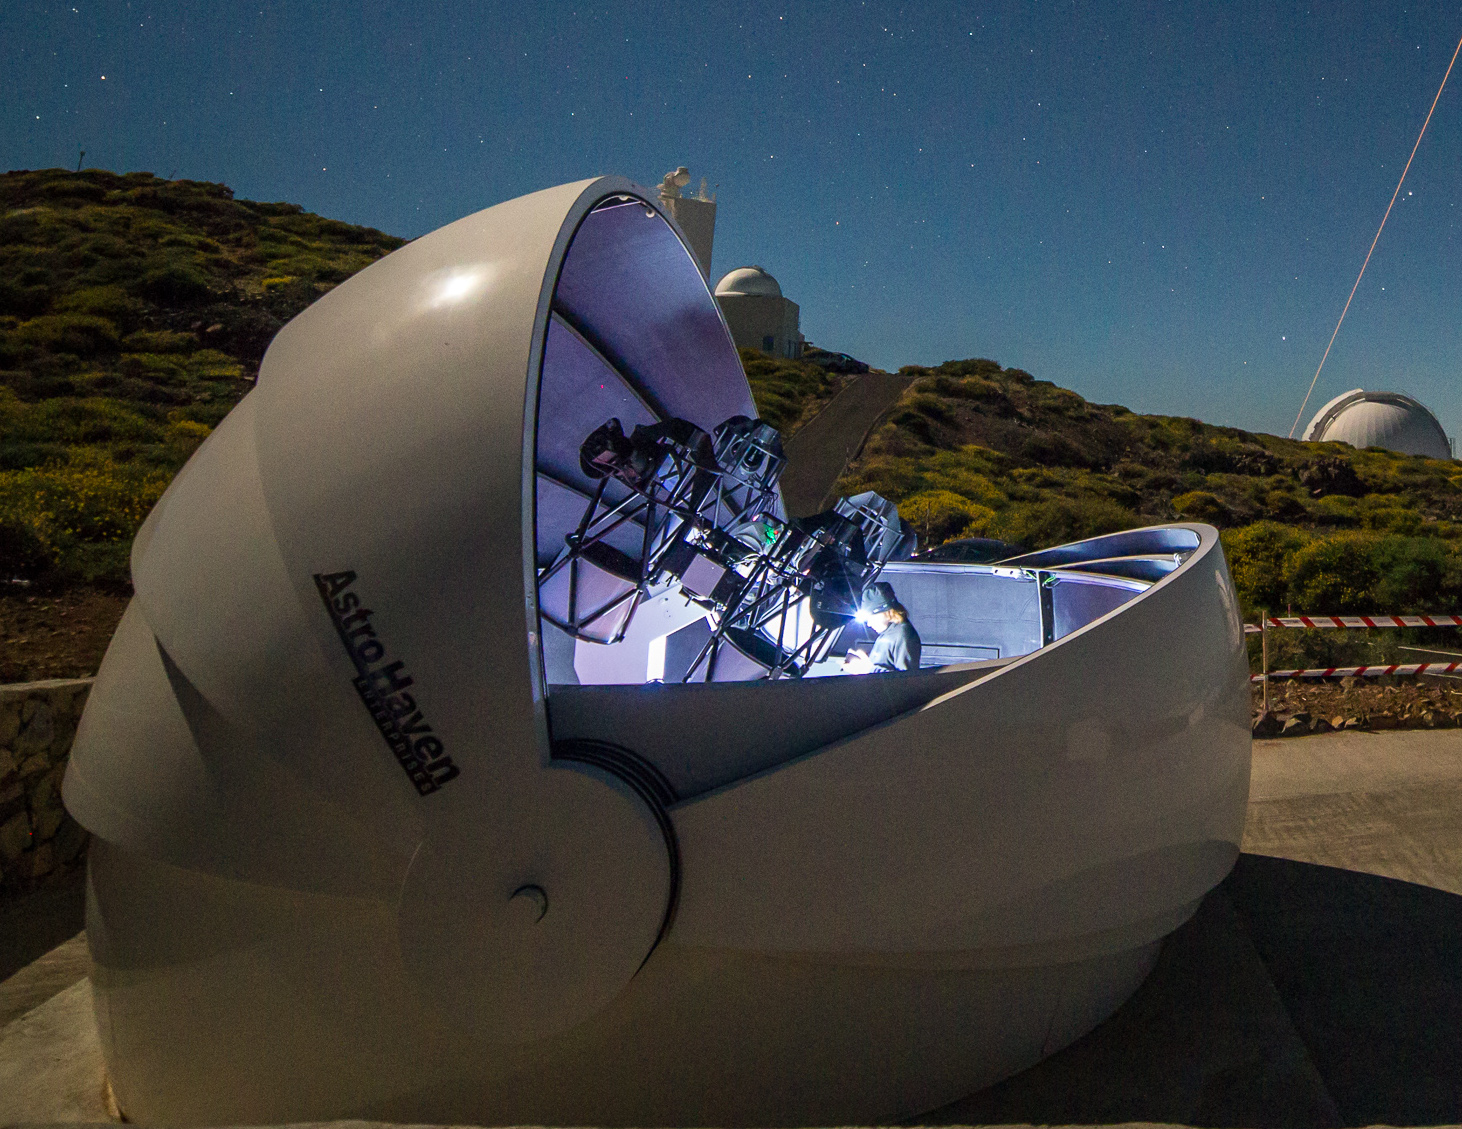
\includegraphics[width=11cm]{images/goto_photo.jpg}
\end{center}
\caption[The GOTO prototype instrument]{The GOTO prototype instrument on La Palma, with four of the eventual eight unit telescopes.}
\label{fig:goto_photo}
\end{figure}

\gls{goto} is designed as a robotic, wide-field transient detection telescope. Under normal circumstances the telescope will carry out an all-sky survey, based on a fixed grid of tiles. Each tile corresponds to the \SI{40}{\square\deg} field of view of the 8 \glspl{ut} observing neighbouring patches of sky, as shown in Figure~\ref{fig:tiles}. The all-sky survey will aim to obtain a high-cadence at an appropriate depth, mapping the entire visible sky several times a week. The high cadence will ensure that there are very recent reference images available to allow detection of objects using difference imaging.

\begin{figure}[htb]
\begin{center}
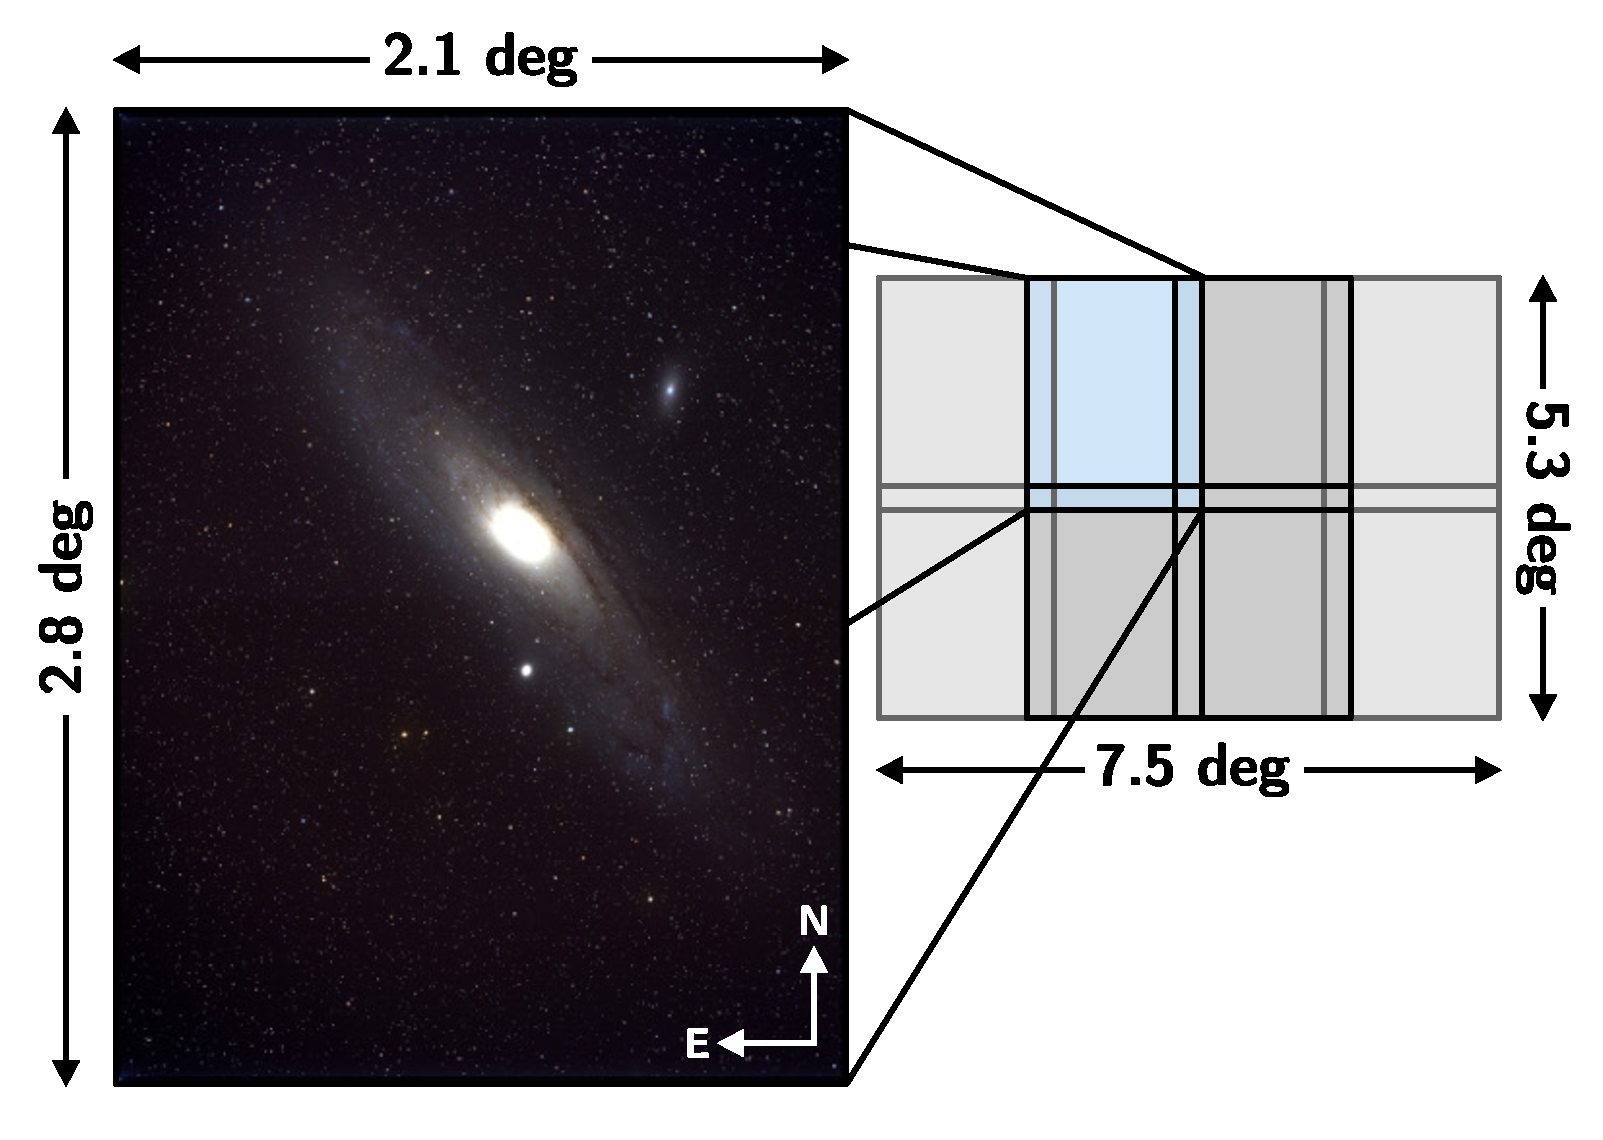
\includegraphics[width=11cm]{images/tiles.pdf}
\end{center}
\caption[M31]{A single commissioning image of M31, showing the wide field of view of each unit telescope. The full 8 unit telescope array will cover an area of approximately 40 square degrees, which forms a single survey tile.}
\label{fig:tiles}
\end{figure}

\end{colsection}

% ~~~~~~~~~~~~~~~~~~~~

\subsection{Motivation}
\label{sec:goto_motivation}
\begin{colsection}

WIP

\end{colsection}

% ~~~~~~~~~~~~~~~~~~~~

\subsection{Design}
\label{sec:goto_design}
\begin{colsection}

WIP

\end{colsection}

% ~~~~~~~~~~~~~~~~~~~~

\subsection{Deployment plan}
\label{sec:goto_expansion}
\begin{colsection}

Starting with 4 in the North, 1 mount.

Then 8 on the 1 mount, soon (TM).

Then another 8.

Then Australia, hopefully.

\end{colsection}

% ~~~~~~~~~~~~~~~~~~~~

\end{colsection}

% ########################################

\chapter{Hardware Characterisation}
\label{chap:hardware}
\chaptoc{}

% ########################################

\newpage
\section{Introduction}
\label{sec:hardware_intro}
\begin{colsection}

In this chapter I detail my work characterising and modelling the GOTO hardware. This work was carried out predominantly in the first year and a half of my PhD, prior to GOTO's commissioning in 2017.
%
\begin{itemize}
    \item In \nref{sec:detectors} I describe and give the results of the detector characterisation tests I ran on the GOTO cameras in the laboratory in Sheffield.
    \item In \nref{sec:throughput} I detail creating a throughput model for the GOTO optical system, in particular examining the Baader filters GOTO uses.
    \item In \nref{sec:photometry} I apply the results of the previous two sections to predict the photometric properties of GOTO images, before comparing them to real observations taken once GOTO was fully operational.
\end{itemize}
%
All work described in this chapter is my own unless otherwise indicated, and has not been published elsewhere.

\end{colsection}

% ########################################

\newpage
\section{Detector properties}
\label{sec:detectors}
\begin{colsection}

% ~~~~~~~~~~~~~~~~~~~~

\begin{colsection}

CCD cameras have a variety of characteristic parameters, including sources of noise. Analysing these under laboratory conditions is important to fully profile them before they are used to take scientific images.

\end{colsection}

% ~~~~~~~~~~~~~~~~~~~~
\subsection{Sources of CCD noise}
\label{sec:noise}
\begin{colsection}

There are many possible sources of noise in images taken with CCD cameras \citep{CCDs}. The most important noise sources for astronomical images are:

\begin{itemize}
    \item \emph{Shot noise} derived from counting photo-electrons from the source object.
    \item \emph{Dark current noise} from thermally generated electrons within the sensor.
    \item \emph{Read-out noise} from the camera electronics.
    \item \emph{Fixed-pattern noise} from different sensitivities between pixels.
    \item \emph{Bias count}, a fixed level of output for each pixel.
\end{itemize}

The shot noise ($\sigma_\text{O}$) arises as photons from the target object arrive at the sensor at different times. The photon arrival time is a Poisson distribution, and if the number of electrons counted is $N$ for large numbers it tends towards a Gaussian distribution with mean $N$ and standard deviation $\sigma_O = \sqrt{N}$. When carrying out on-sky astronomical observations the source noise is typically divided into noise from the target object and noise from the background sky, but that is not relevant in this section.

Dark current noise ($\sigma_\text{D}$) is due to electrons produced by thermal excitations, these are indistinguishable from photo-electrons and will increase with exposure time. As this is also a photon counting measurement it also follows a Poisson distribution, so the noise $\sigma_D = \sqrt{D}$ where $D$ is the dark current per pixel. The dark current depends on temperature, and cooling the cameras will reduce the thermal excitations.

\newpage

Read-out noise ($\sigma_\text{RO}$) depends on the speed data is read out from the CCD.\ The FLI MicroLine cameras read out at a fixed \SI{8}{\mega\hertz}, but other astronomical cameras have variable read-out speeds. As a property of the output electronics the read-out noise is independent of signal or the exposure time used, and therefore it can be represented by a constant value, $\sigma_R = R$, measured in electrons. The MicroLine cameras have two channels with independent readouts, so each will have an independent read-out noise.

Fixed-pattern noise ($\sigma_\text{FP}$) is due to the small differences in size and response between pixels. It it increases linearly with the electron count, including both source and dark electrons (the fixed-pattern noise can be further broken down into the photo response non-uniformity and dark signal non-uniformity, but we will consider it as a single noise source). It can be parametrised as $\sigma_\text{FP} = k_\text{FP}(N+D)$ where $k_\text{FP}$ is a dimensionless constant of proportionality describing the fixed-pattern noise as a percentage of the full-well capacity. Scientific CCD cameras typically have very small non-uniformities between pixels, so $k_\text{FP}$ is usually $<1\%$, but this noise source can dominate when the signal count is high. It can however be removed by flat fielding, so contribution from the fixed-pattern noise is negligible in calibrated astronomical images.

Finally, the bias level is a fixed output of counts from each pixel, and is entirely independent of the input signal. It is therefore the easiest noise source to account for, as once a master bias frame has been constructed it can simply be subtracted from each frame. The MicroLine cameras also include an overscan region (see \aref{sec:chip_layout}), which gives an independent measurement of the bias level for every image.

The noises described above (aside from the bias) are all independent Gaussian random variables, and therefore are added in quadrature to get the total noise per pixel

\begin{equation}
    \begin{split}
        \sigma_\text{Total}^2 & = \sigma_\text{O}^2 +
                                  \sigma_\text{DC}^2 +
                                  \sigma_\text{RO}^2 +
                                  \sigma_\text{FP}^2 \\
                              & = N + D + R^2 + k_\text{FP}^2{(N+D)}^2.
    \end{split}
    \label{eq:noise}
\end{equation}

\end{colsection}

% ~~~~~~~~~~~~~~~~~~~~
\newpage
\subsection{In-lab tests}
\label{sec:camera_tests}
\begin{colsection}

The initial deployment of GOTO was delayed for several months, due to delays on-site at the observatory on La Palma and manufacturing the unit telescopes. The cameras however had already been purchased from FLI, and the delay gave time to test them in the lab in Sheffield. The second set of cameras were also purchased long before the second four unit telescopes were built, these were also bought to Sheffield so the same tests could be repeated.

A list of the nine FLI cameras bought for GOTO is given in \aref{tab:cameras}. Each camera is given a name (Camera 1, Camera 2 etc.) based on the order of their serial numbers. These do not match which GOTO unit telescope they were assigned to, and the cameras on La Palma are sometimes swapped around to allow for repairs.

The first set of four cameras arrived in Warwick in February 2016, and one (Camera 2) was bought to Sheffield in March with a collection of other hardware. The other three were delivered in May and Camera 2 was returned to Warwick, these three were returned in June. The second set cameras were delivered to Warwick in April 2018: four for the next four unit telescopes as well as a spare. The second four cameras (5--8) were brought to Sheffield in May, with Warwick keeping the spare for their own use, these were returned in June.

\begin{table}[t]
    \begin{center}
        \begin{tabular}{c|ccc} %chktex 44
            Name     & Serial number & Set & Tested \\
            \midrule
            Camera 1 & ML0010316     &   1 & May---June 2016  \\
            Camera 2 & ML0330316     &   1 & March---May 2016 \\
            Camera 3 & ML0420516     &   1 & May---June 2016  \\
            Camera 4 & ML0430516     &   1 & May---June 2016  \\
            Camera 5 & ML5644917     &   2 & May---June 2018  \\
            Camera 6 & ML6054917     &   2 & May---June 2018  \\
            Camera 7 & ML6094917     &   2 & May---June 2018  \\
            Camera 8 & ML6304917     &   2 & May---June 2018  \\
            Camera 9 & ML6314917     &   2 & N/A              \\
        \end{tabular}
    \end{center}
    \caption[List of GOTO cameras]{
        A list of the 9 GOTO cameras, with assigned names, serial numbers and dates when the tests were carried out.
    }\label{tab:cameras}
\end{table}

The characterisation tests consisted of taking a series of calibration frames with each camera. Three types of images were needed:

\begin{itemize}
    \item Zero-second dark exposures, to construct bias frames (see \aref{sec:bias}).
    \item Long (30 minute) dark exposures at different temperatures, to measure the dark current (see \aref{sec:dc}).
    \item Flat illuminated frames at different exposure times, to construct photon transfer curves (see \aref{sec:ptc}) and measure linearity (see \aref{sec:lin}).
\end{itemize}

The cameras were tested using two different test setups. \aref{fig:dark_photo} shows the setup for taking dark frames: the cameras are face down and covered. The long dark exposures were taken overnight to as much as possible reduce any excess light reaching the detectors. The flat frames were harder to take. A LCD monitor showing a dark screen was used, with sheets of paper between the camera and the monitor to reduce the illumination. This is shown in \aref{fig:flat_photo}.

The camera manufacturer \glsfirst{fli} and detector manufacturer ON Semiconductor both produce specification sheets advertising expected parameters\footnote{ML50100 available at \url{http://www.flicamera.com/spec_sheets/ML50100.pdf}}\textsuperscript{,}\footnote{KAF-50100 available at \href{http://www.onsemi.com/pub/Collateral/KAF-50100-D.PDF}{\texttt{http://www.onsemi.com/pub/Collateral/KAF-50100-D.pdf}}}, and FLI carried out a limited series of tests on the cameras before selling them. Carrying out our own tests ensures that the cameras meet the specifications, and also allows independent measurements of the key parameters.

\begin{figure}[p]
    \begin{center}
        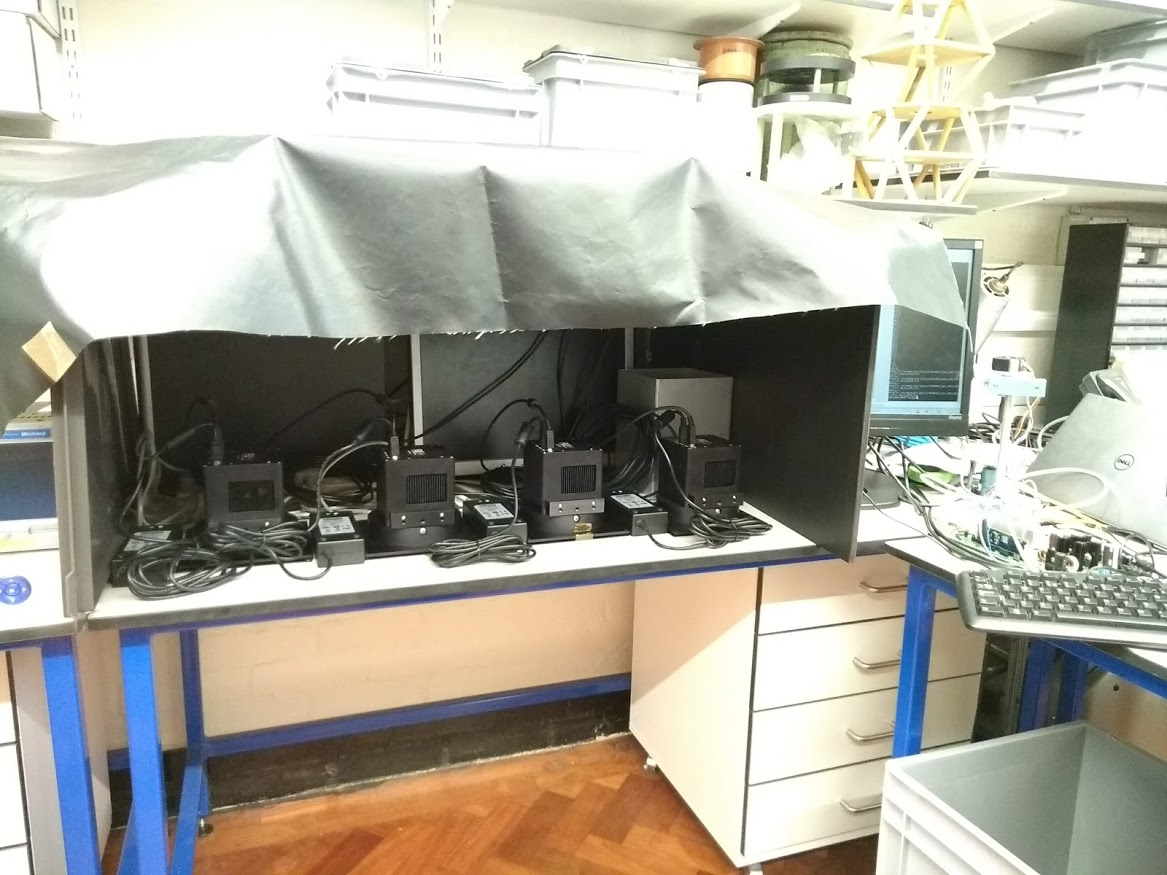
\includegraphics[width=0.75\textwidth]{images/dark_photo.jpg}
    \end{center}
    \caption[The dark frame test setup]{
        A photo of the dark frame test setup in the lab in Sheffield. Dark frames were taken at night with the cover down and ambient light minimised as much as possible.
    }\label{fig:dark_photo}
\end{figure}

\begin{figure}[p]
    \begin{center}
        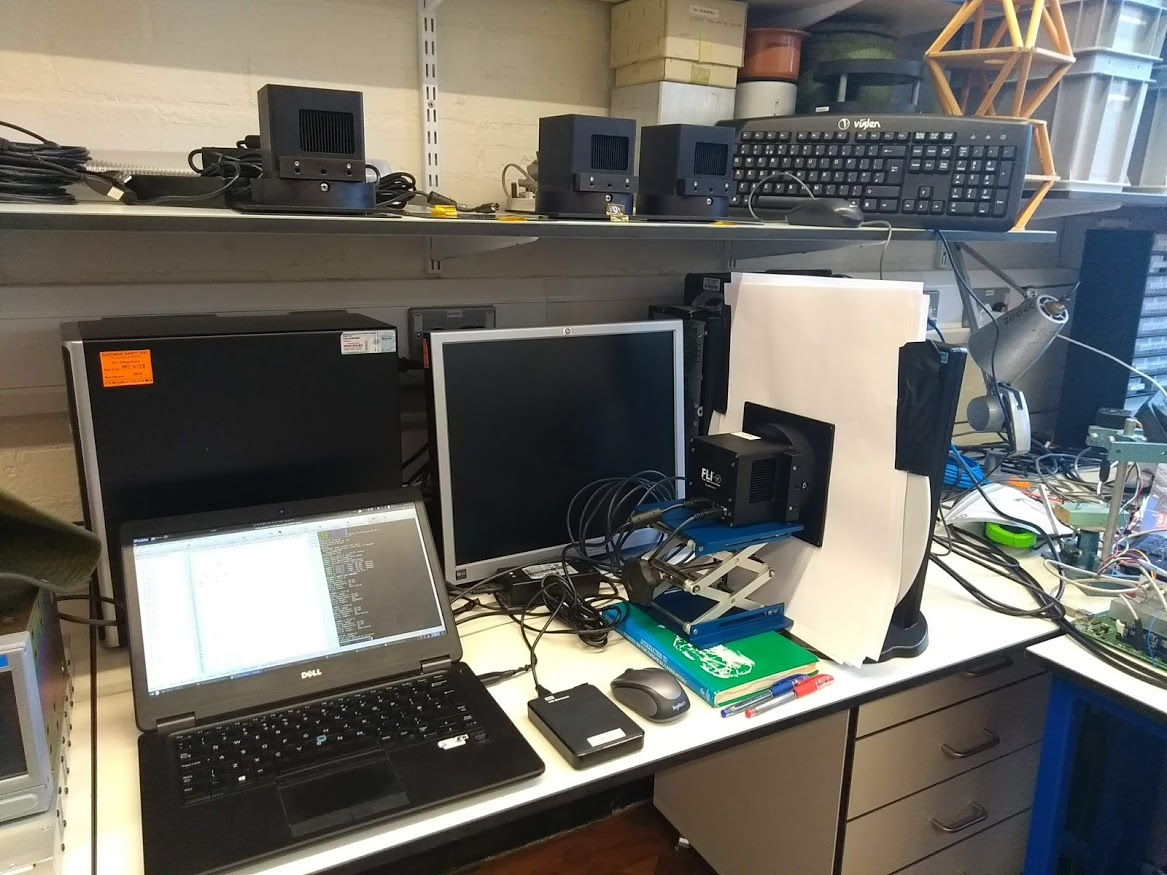
\includegraphics[width=0.75\textwidth]{images/flat_photo.jpg}
    \end{center}
    \caption[The flat frame test setup]{
        A photo of the flat frame test setup. A spare computer monitor was used as a flat screen, with sheets of paper placed in front of the camera to reduce the illumination. The cover shown in \aref{fig:dark_photo} was also placed over the setup.
    }\label{fig:flat_photo}
\end{figure}

\clearpage

\end{colsection}

% ~~~~~~~~~~~~~~~~~~~~
\subsection{Sensor layout}
\label{sec:chip_layout}
\begin{colsection}

The MicroLine ML50100 cameras used by GOTO are contain a KAF-50100 CCD sensor manufactured for FLI by ON Semiconductor\footnote{\url{http://www.onsemi.com/}}. The sensor consists of a 50-megapixel CCD with $\SI{6}{\micro\metre} \times \SI{6}{\micro\metre}$ square pixels. The sensors in the GOTO cameras have two channels each with an independent output, and read out at \SI{8}{\mega\hertz} (variations with four outputs and different readout speeds are also available).

The layout of the sensor is shown in \aref{fig:chip}, adapted from the ON Semiconductor sensor specification sheet. The physical sensor includes $8304 \times 6220$ pixels, while the central region available for data collection has an area of $8176 \times 6132$ pixels. When taking data in full-frame mode the camera outputs an $8304 \times 6220$ array. Surrounding the active area on each edge are 16 \emph{active buffer pixels}, which are light-sensitive but not considered part of the primary region. Around the edge of the active area is a border of light-shielded \emph{dark reference pixels}: 29 dark rows at the start, 26 rows at the end and 28 columns on the sides leading each row. These pixels do not respond to light and therefore can be used as a dark reference. At the beginning and end of each row there is also a test column with 4 blank columns either side, as well as a test row at the end of each frame; these are used to test charge transfer efficiency during the manufacturing process. Finally at the start of each row the register reads out one text pixel, used in the readout process, followed by 10 \emph{dummy pixels} which do not correspond to physical pixels on the sensor. These dummy pixels form an overscan region which can be used to measure the bias level.

A sample frame from Camera 2 is shown in \aref{fig:frame} at high contrast. The extra regions around the frame are visible, including the dark reference and overscan regions.

\begin{figure}[p]
    \begin{center}
        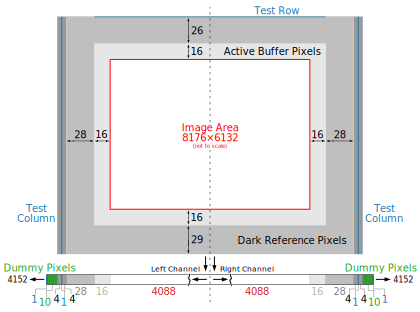
\includegraphics[width=0.85\textwidth]{images/chip}
    \end{center}
    \caption[The layout of the CCD chips in the MicroLine cameras used by GOTO]{
        The layout of the CCD chips in the MicroLine cameras used by GOTO.\@ Note the central image area is not shown to scale.
    }\label{fig:chip}
\end{figure}

\begin{figure}[p]
    \begin{center}
        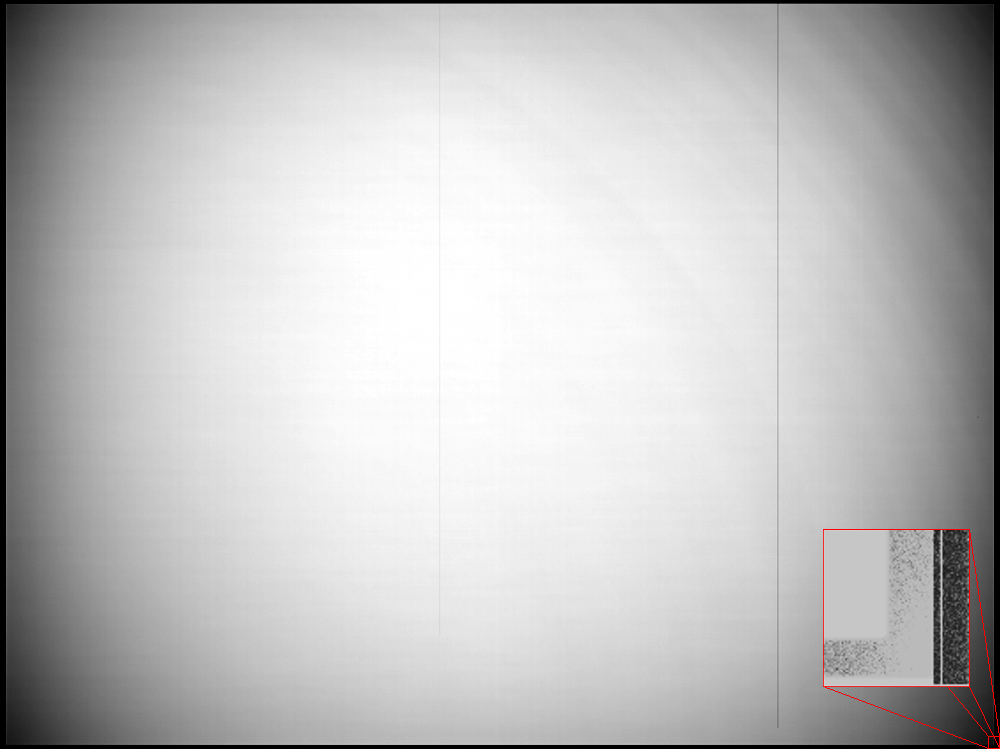
\includegraphics[width=0.7\textwidth]{images/sample.png}
    \end{center}
    \caption[A sample bright frame from one of the MicroLine cameras]{
        A sample bright frame from one of the MicroLine cameras. The highlighted area in the corner shows some of the features described in \aref{fig:chip}.
    }\label{fig:frame}
\end{figure}

\clearpage

\end{colsection}

% ~~~~~~~~~~~~~~~~~~~~
\newpage
\subsection{Bias}
\label{sec:bias}
\begin{colsection}

The bias level is a fixed offset in counts for each pixel. Setting a reasonable bias level in a CCD is important in order to ensure counts are never recorded as negative due to random noise. In general the bias level of each pixel is considered a fixed value, although it can change over time due to degradation of the pixel electronics. Bias should therefore still be measured regularly, as any change might indicate a problem with the detector.

Pixel bias levels can be measured by taking a dark, zero-second exposure time image. This image will not include any electrons from a source, so the shot noise is zero, and as the dark current is proportional to the exposure time this will also be minimised. The image will however still include random read-out noise, so to account for this multiple images are taken and then averaged to produce a master bias frame.

For each of the eight cameras 50 bias images were taken, these were combined to form a master bias frame by taking the median value in each pixel (to account for superfluous counts due to cosmic rays). The mean count in a 2000$\times$2000 pixel region in the centre of each of the two camera channels was measured, using a one-sigma clip to exclude any defect pixels (see \aref{sec:defects}). These values are given in \aref{tab:bias}.

The measured biases are all around the same level, 970--1010 counts, as would be expected. They also have a uniform standard deviation of approximately 0.3--0.4\% of the signal, which will come from the fixed-pattern noise (see \aref{sec:ptc}).

\begin{table}[t]
    \begin{center}
        \begin{tabular}{c|rr} %chktex 44
             & \multicolumn{2}{c}{Bias} \\
             & \multicolumn{2}{c}{(ADU)} \\
             & \multicolumn{1}{c}{L} & \multicolumn{1}{c}{R} \\
            \midrule
            Camera 1 & $971\pm4$ & $969\pm4$ \\
            Camera 2 & $989\pm3$ & $983\pm3$ \\
            Camera 3 & $1004\pm3$ & $991\pm3$ \\
            Camera 4 & $974\pm3$ & $1008\pm4$ \\
        \end{tabular}
        \hspace{0.5cm}
        \begin{tabular}{c|rr} %chktex 44
             & \multicolumn{2}{c}{Bias} \\
             & \multicolumn{2}{c}{(ADU)} \\
             & \multicolumn{1}{c}{L} & \multicolumn{1}{c}{R} \\
            \midrule
            Camera 5 & $994\pm3$ & $986\pm3$ \\
            Camera 6 & $984\pm3$ & $991\pm3$ \\
            Camera 7 & $992\pm3$ & $981\pm3$ \\
            Camera 8 & $1008\pm3$ & $1012\pm3$ \\
        \end{tabular}
    \end{center}
    \caption[Bias values]{
        Bias values for each camera.
    }\label{tab:bias}
\end{table}

\end{colsection}

% ~~~~~~~~~~~~~~~~~~~~
\newpage
\subsection{Gain, read-out noise and fixed-pattern noise}
\label{sec:ptc}
\begin{colsection}

The gain, read-out and fixed-pattern noise of a CCD camera can be measured using the \gls{ptc} method \citep{CCDs, PTC}. To construct a photon transfer curve a series of bright exposures of a flat light source were taken with varying exposure times. For these images the dark current noise is negligible, so once the images has the bias level subtracted the total number of electrons in each pixel, $N_\text{Total}$, will include a number of photo-electrons from the source $N$ plus extra electrons from the readout electronics $R$:

\begin{equation}
    N_\text{Total} = N + R.
    \label{eq:total_count}
\end{equation}

The noise per pixel, excluding dark current, is given by \aref{eq:noise} as

\begin{equation}
    \begin{split}
        \sigma_\text{Total}^2 & = N + R^2 + k_\text{FP}^2 N^2 \\
                              & = N_\text{Total} - R + R^2 + k_\text{FP}^2{(N_\text{Total} - R)}^2.
    \end{split}
    \label{eq:ptc_noise1}
\end{equation}

The counts and total noise here are all in electrons (\elec), however the output of the camera analog-to-digital converter is a digital signal, $S$, measured in \gls{adu}. This signal is linearly related to the actual number of electrons detected $N_\text{Total}$ through the gain $g$, in \elec/ADU, as

\begin{equation}
    N_\text{Total} = g S.
    \label{eq:gain}
\end{equation}

The gain is an important parameter of a CCD detector, and can be set to best utilise the dynamic range of the detector. The KAF-50100 detectors have a specification full well capacity of 40,300 electrons before they saturate, and the cameras have a 16-bit readout (meaning the signal from each pixel can vary from 0 to 65535 ($2^{16}$) ADU). Therefore if the gain was set to $1$ \elec/ADU a saturated pixel would produce a signal of 40300 ADU, which is only using two-thirds of the dynamic range. The ideal gain to utilise the full well capacity for these cameras would therefore be $0.62$ \elec/ADU.\@ However, a high gain introduces a quantisation error due to the random electrons produced by the read-out noise. Setting the gain therefore is a balance between these two effects.

Since \aref{eq:gain} shows the signal $S$ is directly proportional to the number of electrons $N$, their errors are also directly proportional with the same constant. Therefore the noise in the signal, $\sigma_S$, is related to the noise in the total electron count as

\begin{equation}
    \sigma_\text{Total} = g \sigma_S.
    \label{eq:noise_gain}
\end{equation}

Converting the total electron count and noise in \aref{eq:ptc_noise1} into ADU results in

\begin{equation}
    g^2\sigma_S^2 = gS - R + R^2 + k_\text{FP}^2 {(gS - R)}^2,
    \label{eq:ptc_noise2}
\end{equation}

and rearranging this gives the final photon transfer curve equation

\begin{equation}
    \sigma_S^2 = \frac{R^2(1-k_\text{FP}^2) - R}{g^2} + \frac{1}{g}S + k_\text{FP}^2 S^2.
    \label{eq:ptc}
\end{equation}

This is a quadratic equation in $S$ which relates the measured total signal $S$ to the variance in the signal $\sigma_S^2$, where $S$ and $\sigma_S$ are in ADU, read-out noise $R$ is still in \elec, gain $g$ is in \elec/ADU and the fixed-pattern noise parameter $k_\text{FP}$ is dimensionless. Since $k_\text{FP}$ is expected to be a very small fraction, typically less than 1\%, the $(1-k_\text{FP}^2)$ factor is often ignored. As well the constant is often further simplified to just $R^2/g^2$, which could be considered as $R_S^2$ where $R_S$ is measured in ADU.\@ For this test the full equation was used when fitting to the data.

A photon transfer curve is a log-log plot of a signal value against the noise in the signal, here represented by $S$ and standard deviation $\sigma_S$ (the square root of the variance). By fitting \aref{eq:ptc} to this plot values for the gain, read-out noise and fixed-pattern noise can be determined. The key features of a photon transfer curve are common for all CCDs, and are shown in cartoon form in \aref{fig:ptc_cartoon}.

\begin{figure}[t]
    \begin{center}
        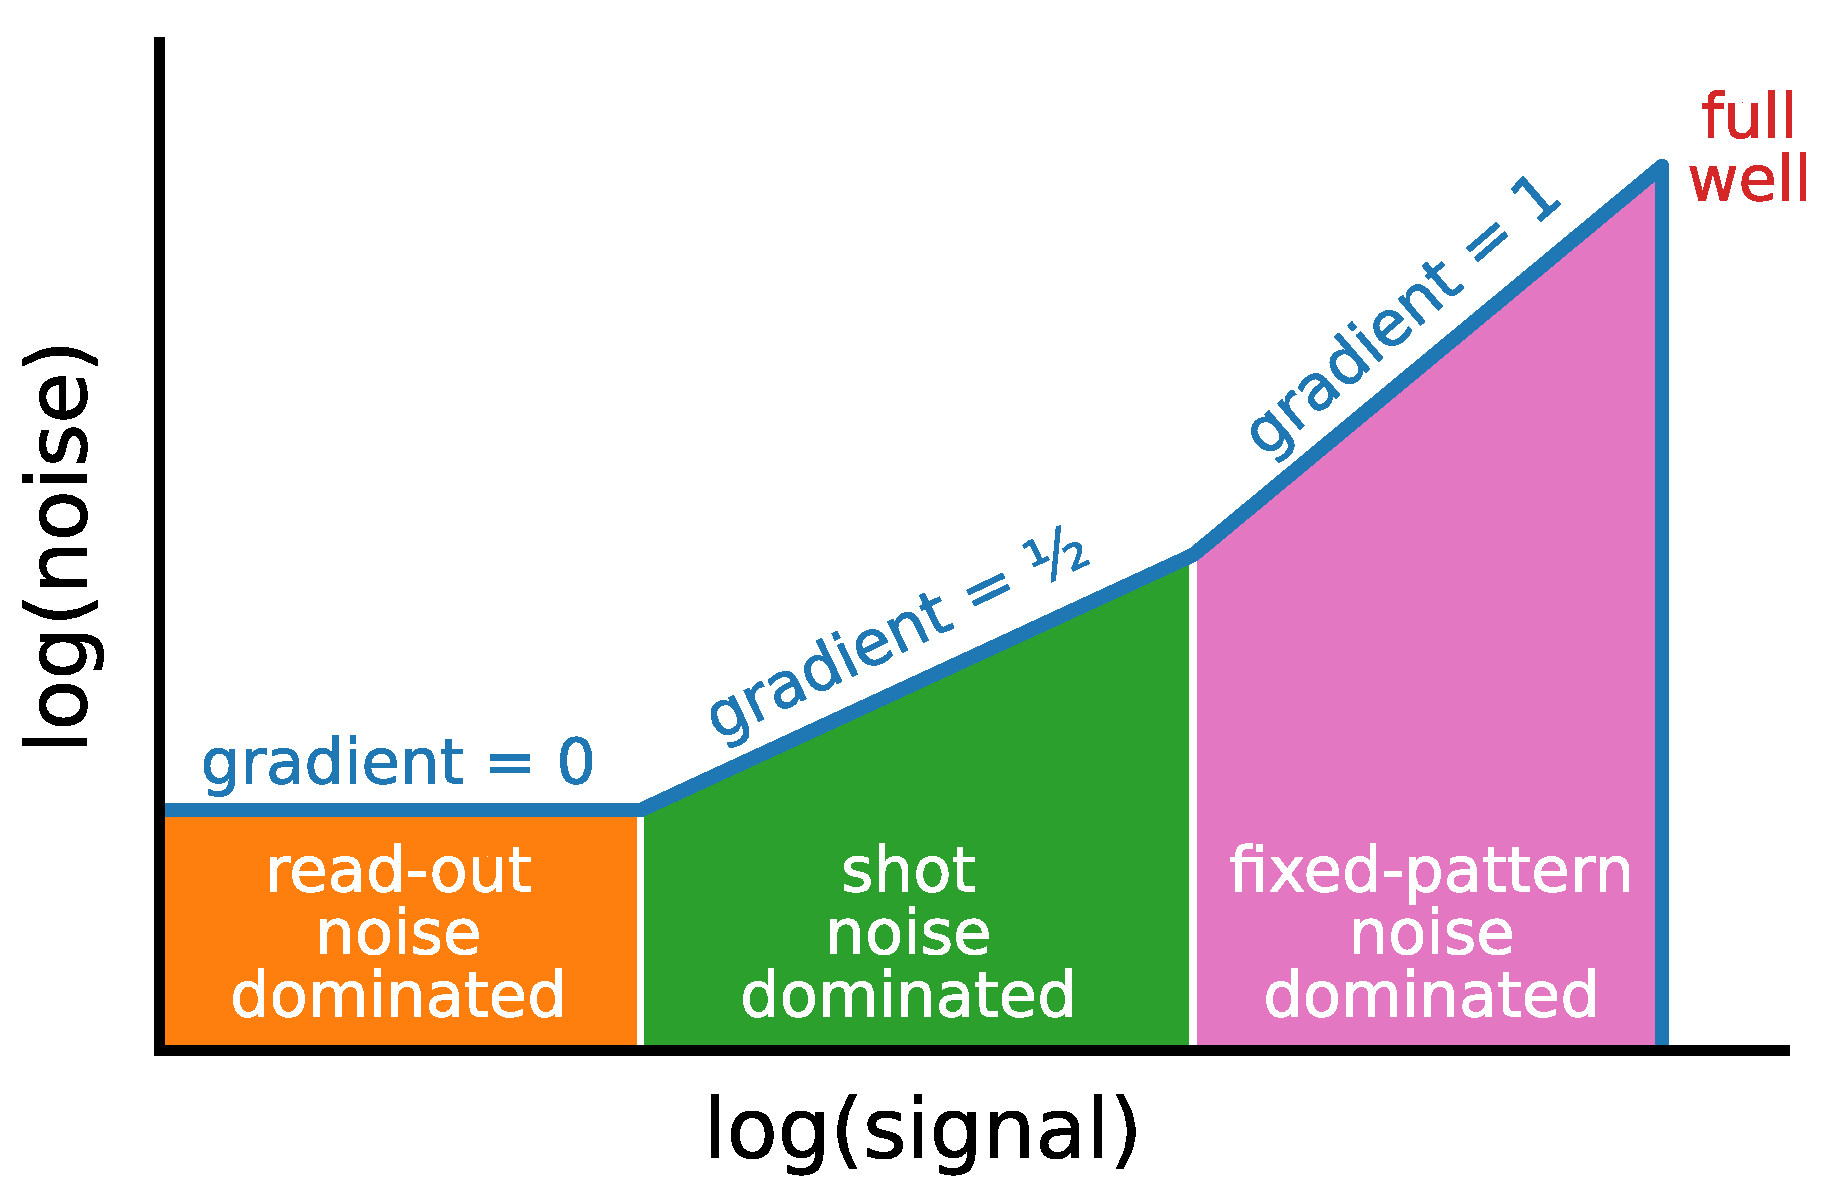
\includegraphics[width=0.75\textwidth]{images/ptc.pdf}
    \end{center}
    \caption[Key features of the photon transfer curve]{
        The key features of a photon transfer curve, adapted from Figure 2.2 of \citet{CCDs}.
    }\label{fig:ptc_cartoon}
\end{figure}

There are three visible noise regimes in the photon transfer curve. The first is when the signal is zero. For small $S$ in \aref{eq:ptc} the noise is constant, and as there is no signal the overall noise is limited by the detector noise. This will include both the read-out noise and the dark current, but as these are very short exposure times (less than 1 second) the dark current is completely negligible and the read-out noise dominates. At higher signals the noise is dominated by the shot noise. As this is proportional to the square root of the signal this region has a gradient of 1/2 when plotted on the log-log axis, and when $\sigma_S$ is zero the signal will equal the gain (i.e.\ the value of the gain is where the linear fit crosses the x-axis). As the signal increases further the fixed-pattern noise begins to dominate over the shot noise, as it is proportional to the signal this produces a gradient of 1 in the \gls{ptc}. Finally the pixel will reach its full well value and saturate, so the noise drops to zero.

As it is impossible to know the exact number of incoming photons on each pixel, it is not possible to determine the signal and noise values for a given pixel. Instead the PTC is constructed by selecting a region of pixels and plotting the mean signal value against the standard deviation. Repeated for several regions across the image this gives a reasonable approximation of the average noise in each pixel.

\begin{table}[t]
    \begin{center}
        \begin{tabular}{l|cc|cc|cc} %chktex 44
             &
            \multicolumn{2}{c|}{Gain} &
            \multicolumn{2}{c|}{RO noise} &
            \multicolumn{2}{c}{FP noise} \\
            &
            \multicolumn{2}{c|}{(\elec/ADU)} &
            \multicolumn{2}{c|}{(\elec)} &
            \multicolumn{2}{c}{(\%)} \\
             & L & R & L & R & L & R \\
            \midrule
            Camera 1 & 0.53 & 0.53 & 12.9 & 12.6 & 0.46 & 0.45 \\
            Camera 2 & 0.53 & 0.53 & 12.4 & 12.2 & 0.44 & 0.46 \\
            Camera 3 & 0.57 & 0.57 & 13.1 & 12.3 & 0.45 & 0.42 \\
            Camera 4 & 0.57 & 0.58 & 14.0 & 14.5 & 0.41 & 0.43 \\
            Camera 5 & 0.62 & 0.63 & 12.8 & 13.3 & 0.40 & 0.40 \\
            Camera 6 & 0.63 & 0.62 & 12.4 & 13.1 & 0.40 & 0.40 \\
            Camera 7 & 0.62 & 0.62 & 13.6 & 13.1 & 0.41 & 0.39 \\
            Camera 8 & 0.62 & 0.62 & 14.8 & 12.8 & 0.41 & 0.39 \\
        \end{tabular}
    \end{center}
    \caption[Gain, read-out noise and fixed-pattern noise values]{
        Gain, read-out noise and fixed-pattern noise values found by fitting photon transfer curves for each camera.
    }\label{tab:ptc}
\end{table}

\glspl{ptc} were constructed for all eight cameras, by taking flat images of varying exposure times. Twelve 50$\times$50 pixel regions were selected across the field, and the mean and standard deviation of the pixel values were plotted to form the \gls{ptc}. These are shown in \aref{fig:ptcs}. The curves were fitted to \aref{eq:ptc}, and the resulting values for the gain ($g$), read-out noise ($R$) and fixed-pattern noise ($k_\text{FP}$) are given in \aref{tab:ptc}.

As expected, the gain values are all around 0.6 \elec/ADU, and would have been set as such to maximise the dynamic range. There is a clear difference in gain levels between the first set of cameras (1--4) and the second set (5--8), which is most likely due to changes made by FLI over the two years between their manufacture.

The read-out noise values match the FLI specifications which advertises a typical system noise of 12 \elec{} when reading out at \SI{8}{\mega\hertz}. The two channels on each camera are independent and therefore there is no correlation in read-out noise, unlike the gain which is always approximately the same in each amplifier.

Finally, as expected the fixed-pattern noise is a low fraction of the signal. It notably decreases from $\sim$0.45\% to $\sim$0.40\%; if this is related to improved chip manufacturing this may be related to the change in gain in the later cameras. However, this test only includes a small sample of the 50 million pixels on each chip and so may not be a perfect measure of the overall photo response non-uniformity. The values for the fixed-pattern noise also match the standard deviations measured in the master biases in \aref{sec:bias}.

\begin{figure}[p]
    \begin{center}
        \begin{minipage}[t]{0.49\textwidth}\vspace{10pt}
            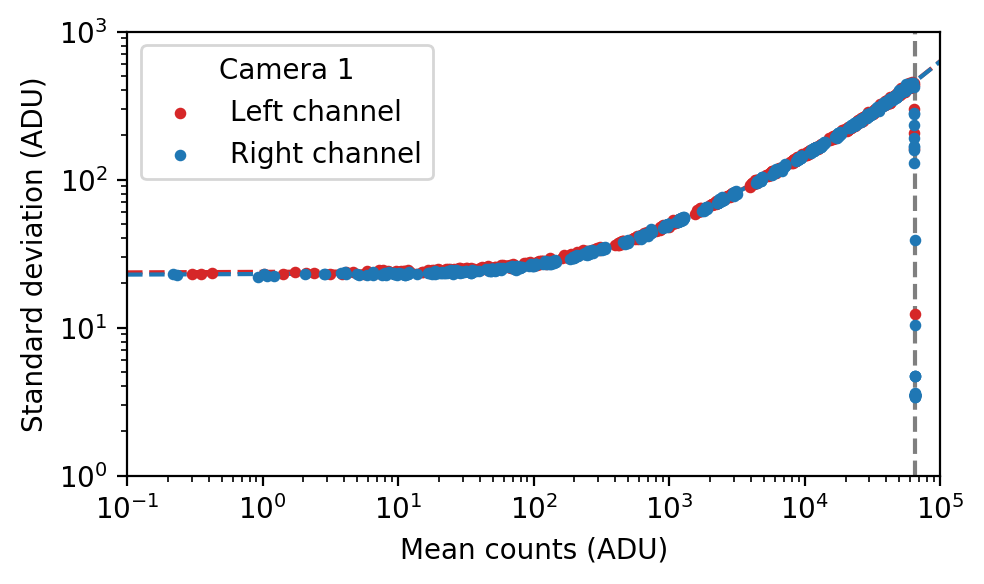
\includegraphics[width=\linewidth]{images/detectors/ptc_1.png}
        \end{minipage}
        \begin{minipage}[t]{0.49\textwidth}\vspace{10pt}
            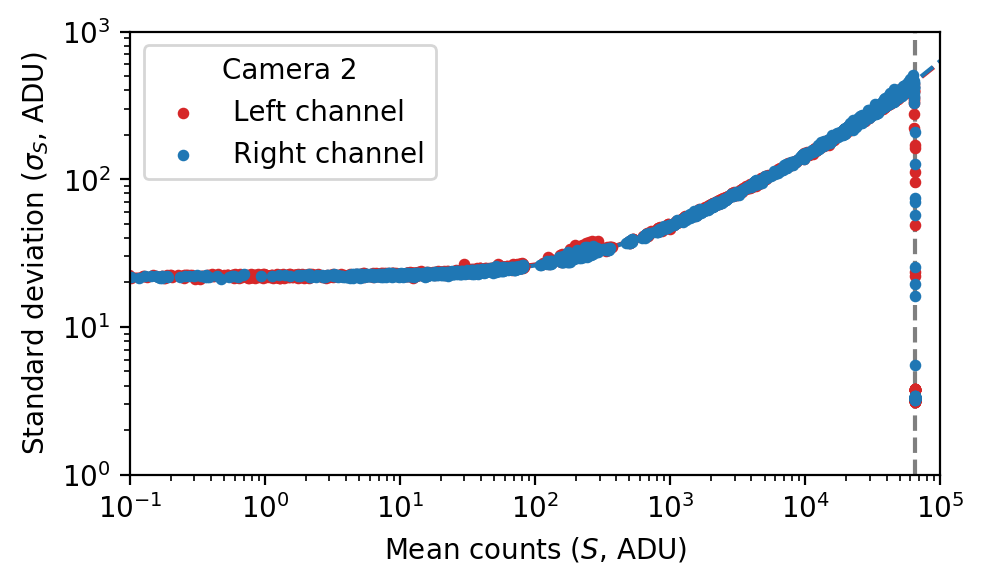
\includegraphics[width=\linewidth]{images/detectors/ptc_2.png}
        \end{minipage}

        \begin{minipage}[t]{0.49\textwidth}\vspace{10pt}
            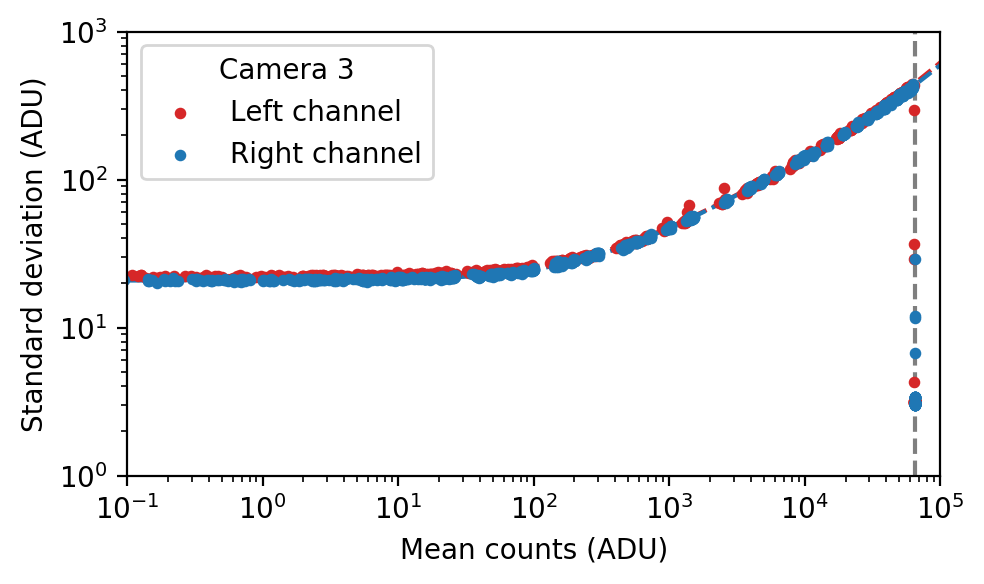
\includegraphics[width=\linewidth]{images/detectors/ptc_3.png}
        \end{minipage}
        \begin{minipage}[t]{0.49\textwidth}\vspace{10pt}
            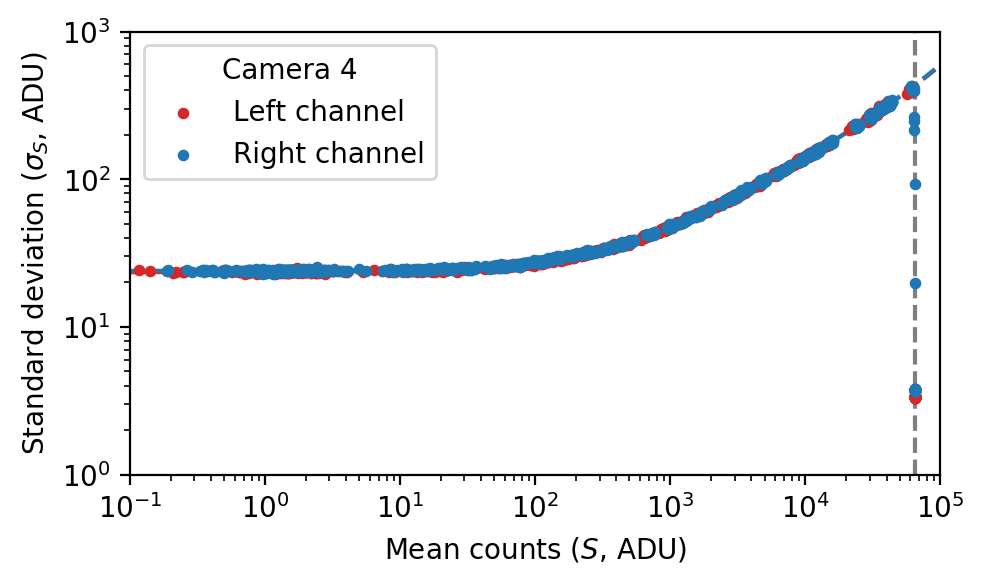
\includegraphics[width=\linewidth]{images/detectors/ptc_4.png}
        \end{minipage}

        \begin{minipage}[t]{0.49\textwidth}\vspace{10pt}
            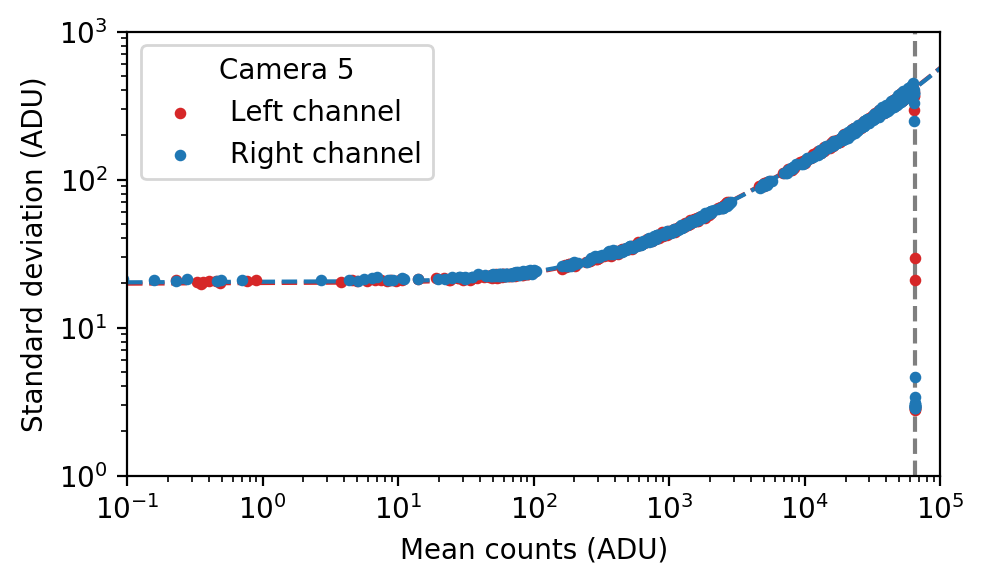
\includegraphics[width=\linewidth]{images/detectors/ptc_5.png}
        \end{minipage}
        \begin{minipage}[t]{0.49\textwidth}\vspace{10pt}
            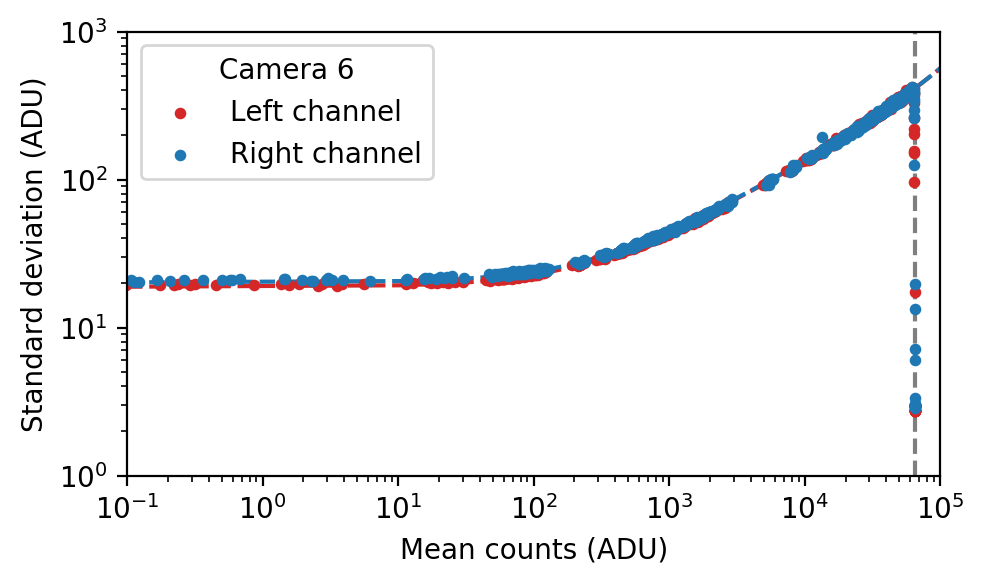
\includegraphics[width=\linewidth]{images/detectors/ptc_6.png}
        \end{minipage}

        \begin{minipage}[t]{0.49\textwidth}\vspace{10pt}
            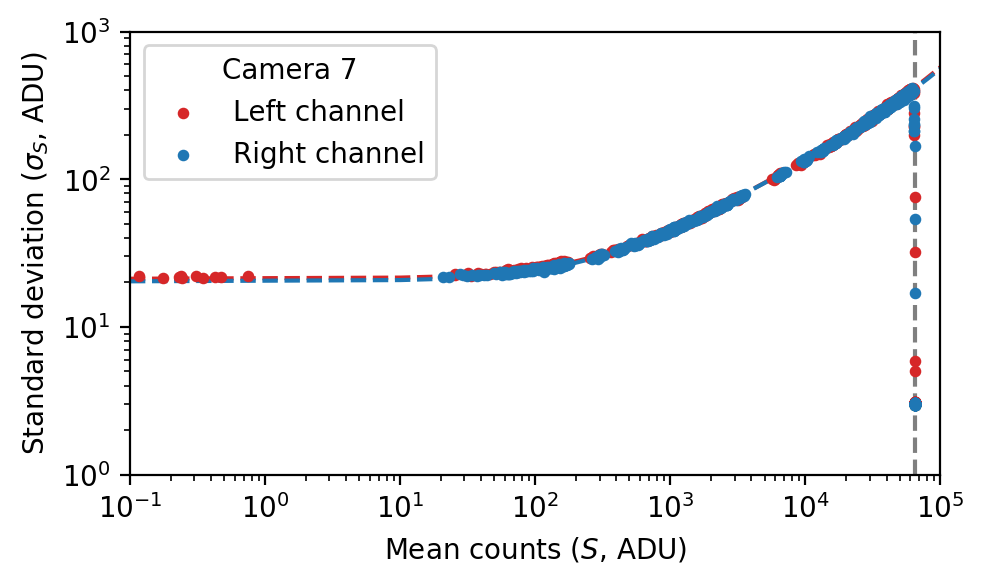
\includegraphics[width=\linewidth]{images/detectors/ptc_7.png}
        \end{minipage}
        \begin{minipage}[t]{0.49\textwidth}\vspace{10pt}
            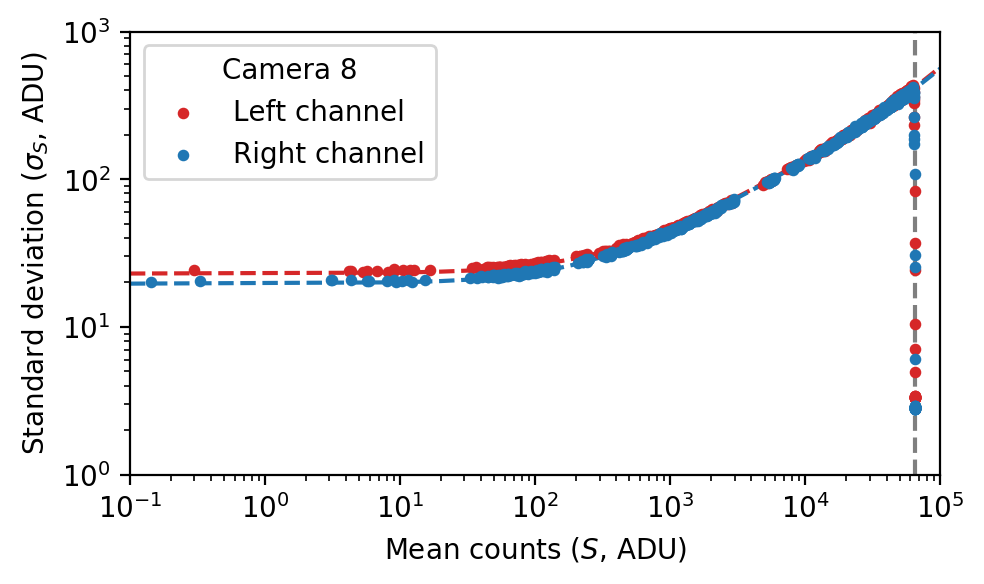
\includegraphics[width=\linewidth]{images/detectors/ptc_8.png}
        \end{minipage}
    \end{center}
    \caption[Photon transfer curve plots]{
        Photon transfer curve plots for each camera.
    }\label{fig:ptcs}
\end{figure}

\clearpage

\end{colsection}

% ~~~~~~~~~~~~~~~~~~~~
\newpage
\subsection{Dark current}
\label{sec:dc}
\begin{colsection}

Dark current is another source of noise in a CCD, produced by thermally excited electrons \citep{dark_current}. The dark current noise is therefore independent of the incoming signal or the exposure time, but increases as a function of temperature, $T$. Specifically the dark current increases at an exponential rate and so can be modelled in the form

\begin{equation}
    D(T) = Ae^{kT + C}
    \label{eq:dark_model}
\end{equation}

where $A$, $k$ and $C$ are constants. Dark current is usually defined as doubling after a fixed increase in temperature called the doubling temperature, $T_d$, so that if the dark current $D(T_0) = D_0$ then $D(T_0 + T_d) = 2D_0$. Redefining \aref{eq:dark_model} using these constants gives the equation for dark currant as

\begin{equation}
    D(T) = D_0 e^{\frac{\ln(2)}{T_d}(T + T_0)}.
    \label{eq:dc}
\end{equation}

The choice of $T_0$ is arbitrary, and is usually decided as a reasonable operating temperature by the CCD manufacturer. The FLI specifications give a value for the typical dark current at \SI{-25}{\celsius}, so that is the value of $T_0$ used in this test.

The MicroLine cameras have an in-built fan cooler which can reach \SI{40}{\celsius} below the ambient temperature. In order to find values for the dark current $D_0$ and doubling temperature $T_d$, a series of long (30 minute) dark exposures were taken with each camera at varying temperatures. The mean pixel count was then measured, and divided by 1800 to get the dark current in ADU/second. This value was plotted against temperature as shown in \aref{fig:dcs}. The points were fitted to \aref{eq:dc}, and the resulting values for the dark current and doubling temperature are given in \aref{tab:dc}.

\begin{table}[t]
    \begin{center}
        \begin{tabular}{c|cc|cc|rr} %chktex 44
             &
            \multicolumn{4}{c|}{Dark current per pixel} &
            \multicolumn{2}{c}{Doubling} \\
             &
            \multicolumn{4}{c|}{at \SI{-25}{\celsius}} &
            \multicolumn{2}{c}{temperature} \\
             &
            \multicolumn{2}{c|}{(ADU/s)} &
            \multicolumn{2}{c|}{(e-/s)} &
            \multicolumn{2}{c}{(\SI{}{\celsius})} \\
             & L & R & L & R &
             \multicolumn{1}{c}{L} & \multicolumn{1}{c}{R} \\
            \midrule
            Camera 1 & 0.0022 & 0.0017 & 0.0012 & 0.0009 &  7.9 &  6.7 \\
            Camera 2 & 0.0030 & 0.0027 & 0.0016 & 0.0014 &  8.9 &  8.2 \\
            Camera 3 & 0.0034 & 0.0036 & 0.0019 & 0.0020 & 10.7 & 10.9 \\
            Camera 4 & 0.0026 & 0.0030 & 0.0015 & 0.0017 &  9.5 & 10.2 \\
            Camera 5 & 0.0015 & 0.0017 & 0.0009 & 0.0011 &  6.6 &  7.2 \\
            Camera 6 & 0.0020 & 0.0017 & 0.0013 & 0.0011 &  7.5 &  6.8 \\
            Camera 7 & 0.0017 & 0.0014 & 0.0011 & 0.0008 &  7.6 &  6.5 \\
            Camera 8 & 0.0019 & 0.0015 & 0.0012 & 0.0009 &  7.5 &  6.5 \\
        \end{tabular}
    \end{center}
    \caption[Dark current values]{
        Dark current values for each camera. The conversion from ADU/s to \elec/s used the gain values given in \aref{tab:ptc}.
    }\label{tab:dc}
\end{table}

The FLI MicroLine camera specification for dark current changed between the two test periods; initially it gave a typical per-pixel value of 0.002~\elec/s at \SI{-25}{\celsius}, but in between testing the two sets of cameras that was increased to 0.008~\elec/s. In order to convert the fitted value of dark current in ADU/s to e-/s the individual gain values found from the PTC were used, as listed in \aref{tab:ptc}. All the cameras were found to have a dark current well within the revised specification value, and all except Camera 3 are comfortably below the original 0.002~\elec/s specification.

The KAF-50100 specification includes a value for the dark current doubling temperature of \SI{5.7}{\celsius}, the measured values are all higher: between 6.5--\SI{11}{\celsius}. In practice the temperature dependence of the dark current is not important to GOTO, as the cameras are always cooled to \SI{-25}{\celsius} before images are taken and remain steady at that temperature throughout the night.

The dark current was also examined as a function of time since power on, as in some cameras there are a noticeable amount of free electrons left trapped in the lattice which take time to dissipate \citep{Liam}. No such trend was visible using the FLI cameras. Since the MicroLine cameras have the detector and cooler integrated into the same body there has to be some time spent waiting after power on for the camera to cool to the target temperature before any images could be taken, thus negating the effect.

\begin{figure}[p]
    \begin{center}
        \begin{minipage}[t]{0.49\textwidth}\vspace{10pt}
            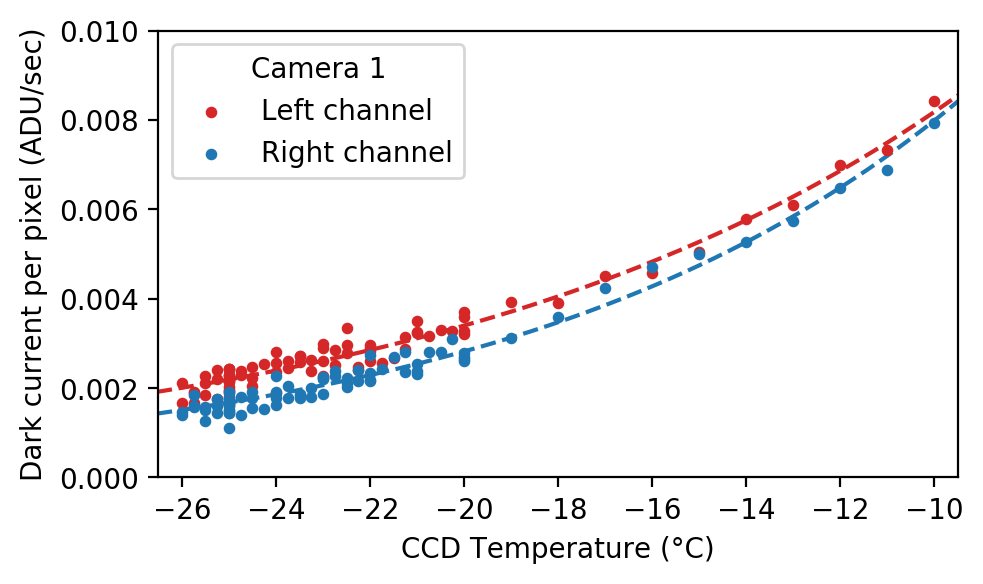
\includegraphics[width=\linewidth]{images/detectors/dc_1.png}
        \end{minipage}
        \begin{minipage}[t]{0.49\textwidth}\vspace{10pt}
            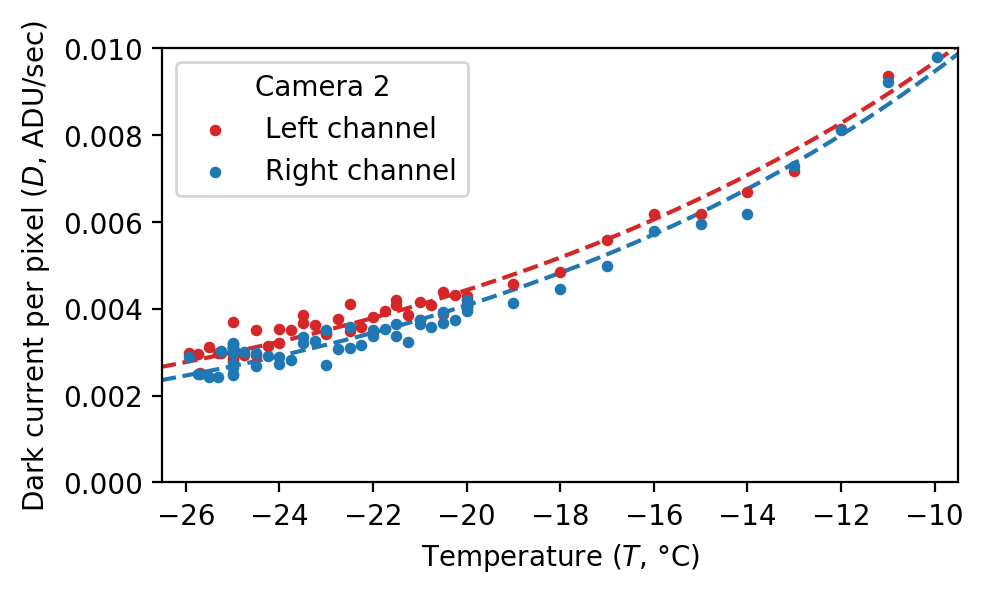
\includegraphics[width=\linewidth]{images/detectors/dc_2.png}
        \end{minipage}

        \begin{minipage}[t]{0.49\textwidth}\vspace{10pt}
            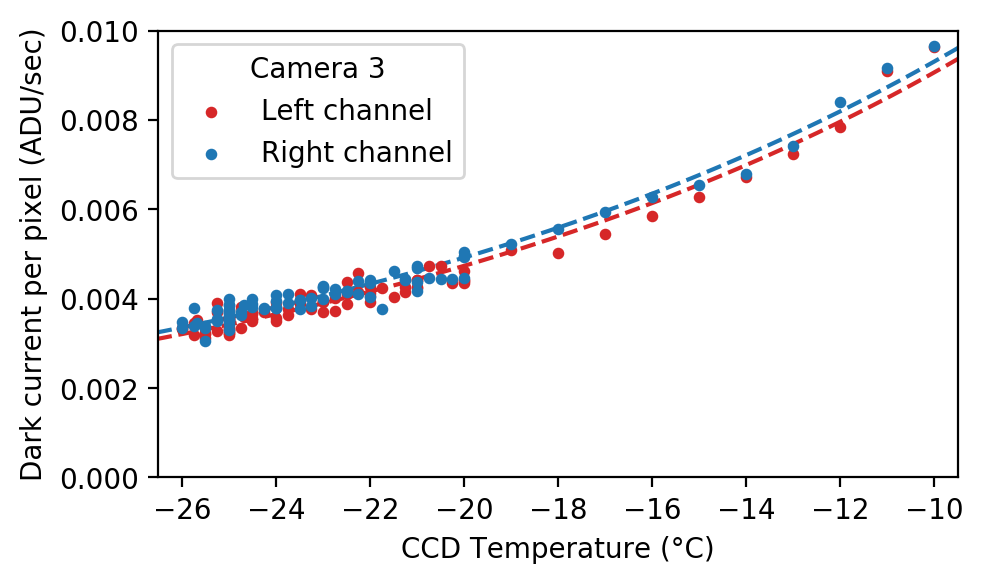
\includegraphics[width=\linewidth]{images/detectors/dc_3.png}
        \end{minipage}
        \begin{minipage}[t]{0.49\textwidth}\vspace{10pt}
            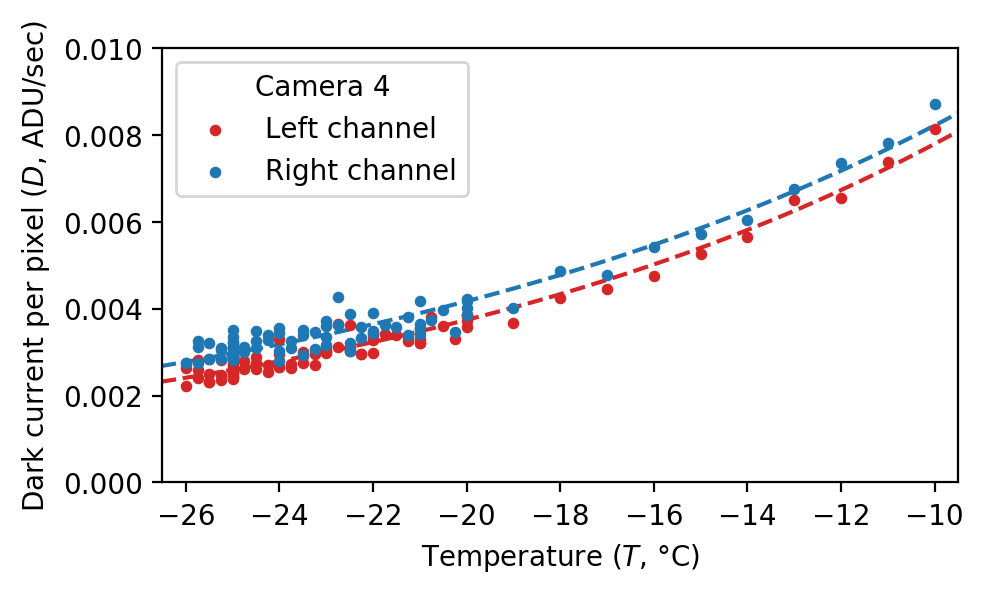
\includegraphics[width=\linewidth]{images/detectors/dc_4.png}
        \end{minipage}

        \begin{minipage}[t]{0.49\textwidth}\vspace{10pt}
            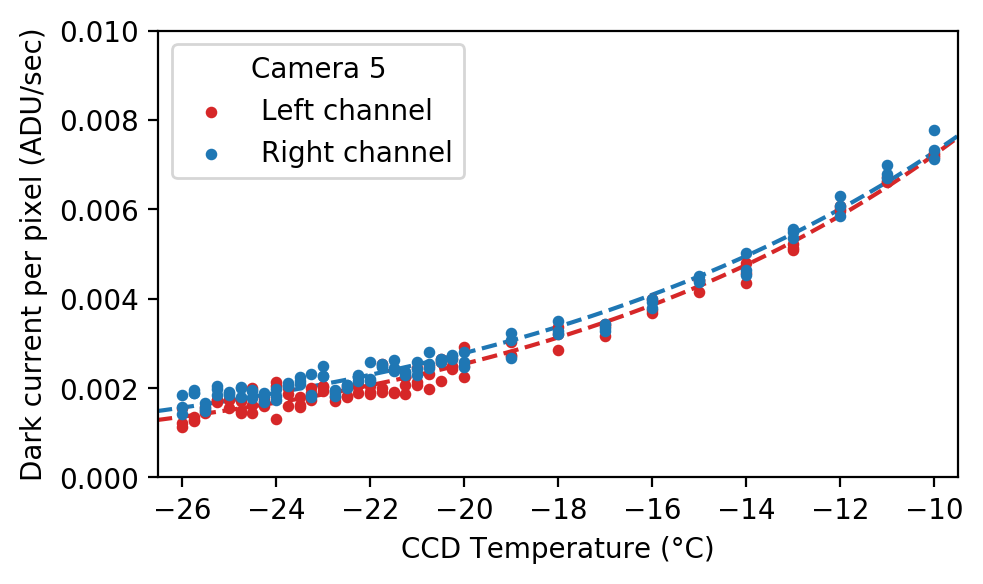
\includegraphics[width=\linewidth]{images/detectors/dc_5.png}
        \end{minipage}
        \begin{minipage}[t]{0.49\textwidth}\vspace{10pt}
            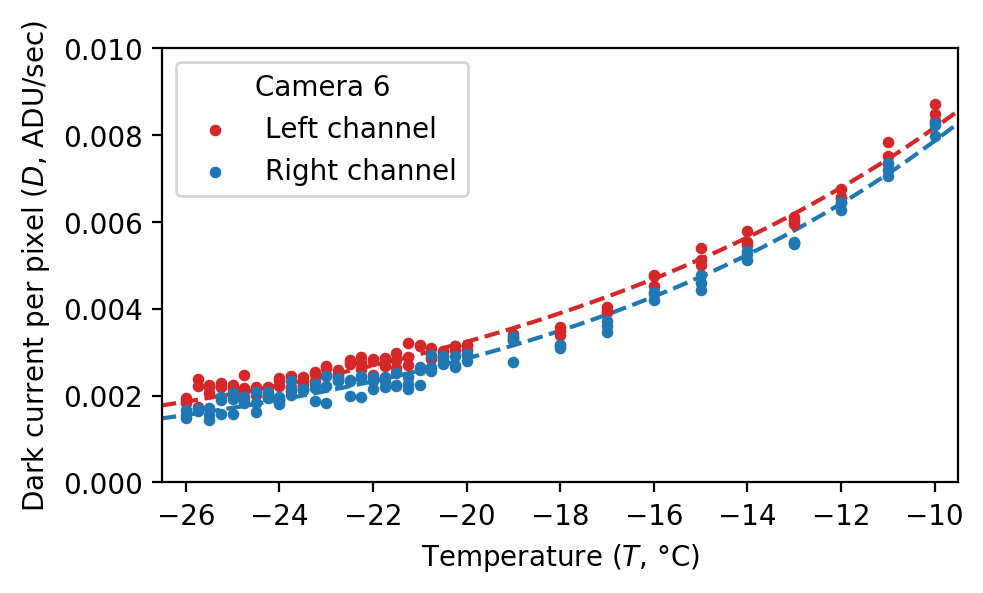
\includegraphics[width=\linewidth]{images/detectors/dc_6.png}
        \end{minipage}

        \begin{minipage}[t]{0.49\textwidth}\vspace{10pt}
            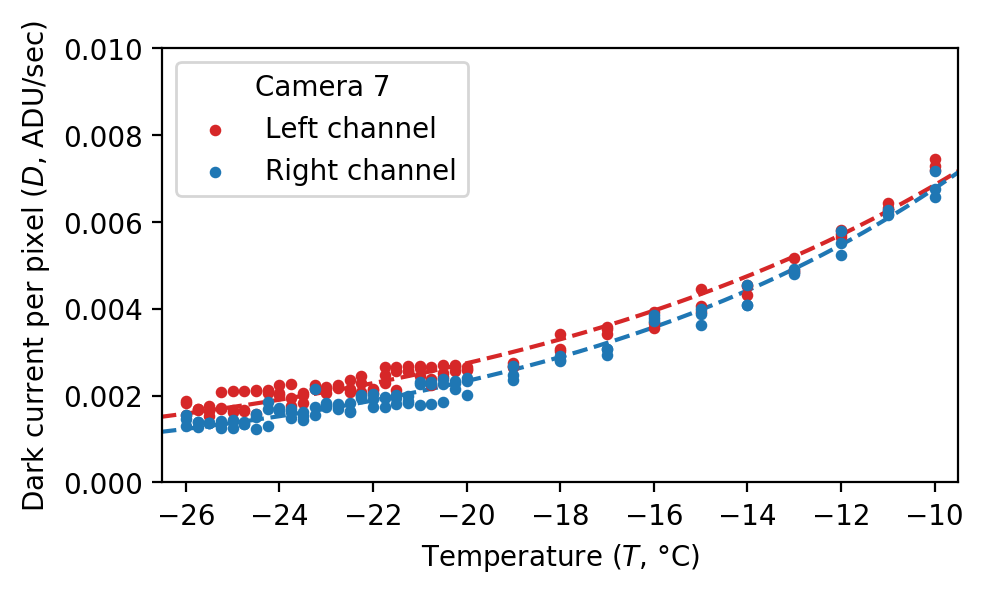
\includegraphics[width=\linewidth]{images/detectors/dc_7.png}
        \end{minipage}
        \begin{minipage}[t]{0.49\textwidth}\vspace{10pt}
            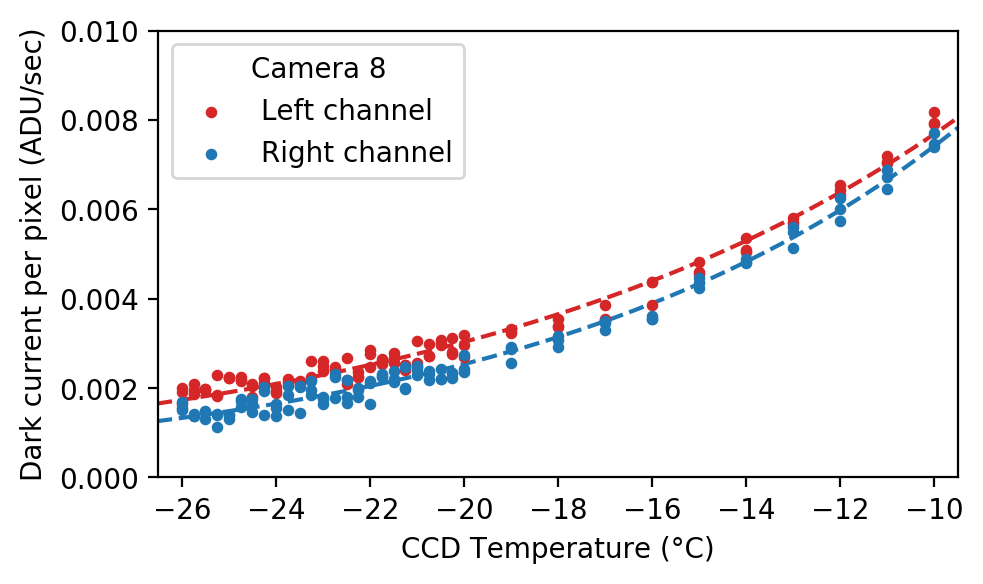
\includegraphics[width=\linewidth]{images/detectors/dc_8.png}
        \end{minipage}
    \end{center}
    \caption[Dark current plots]{
        Dark current plots for each camera.
    }\label{fig:dcs}
\end{figure}

\clearpage

\end{colsection}

% ~~~~~~~~~~~~~~~~~~~~
\newpage
\subsection{Linearity}
\label{sec:lin}
\begin{colsection}

Linearity is a measure of the response of the CCD over its dynamic range. It is particularly important for scientific imaging that the measured counts are directly proportional to the object signal.

The non-linearity of each camera was measured using the same images taken for the photon transfer curves in \aref{sec:ptc}, bright images of a flat source with increasing exposure times. The images were bias-subtracted, and the mean counts of a central 2000$\times$2000 pixel region in the centre of each channel was plotted against the exposure time, shown in \aref{fig:lin}. A linear relation was fitted to the central potion of the data, excluding the upper and lower 10\% of the dynamic range. Residuals from this fit as a percentage of the count are also plotted in \aref{fig:lin}, and the mean absolute deviation from the linear fit over the central region is given in \aref{tab:lin}.

The values for non-linearity measured vary greatly between each camera, and several are over 1\%. If these values were true this would be a major problem when making accurate photometric measurements. However, the FLI specification advertises a non-linearity of <1\%, and FLI's own tests of the cameras consistently report non-linearity of 0.2\% or less. Accurately measuring the response of a CCD requires a perfectly uniform light source and an integrating sphere, which FLI would have access to. I had to make do with a LCD screen when carrying out the tests in the lab, which is a poor substitute. Therefore the values in \aref{tab:lin} should not be considered reliable measurements.

\begin{table}[t]
    \begin{center}
        \begin{tabular}{c|cc} %chktex 44
             & \multicolumn{2}{c}{Non-linearity} \\
             & \multicolumn{2}{c}{(\%)} \\
             & \multicolumn{1}{c}{L} & \multicolumn{1}{c}{R} \\
            \midrule
            Camera 1 & 2.29 & 2.00 \\
            Camera 2 & 0.76 & 0.65 \\
            Camera 3 & 0.34 & 0.39 \\
            Camera 4 & 0.18 & 0.22 \\
        \end{tabular}
        \hspace{0.5cm}
        \begin{tabular}{c|cc} %chktex 44
             & \multicolumn{2}{c}{Non-linearity} \\
             & \multicolumn{2}{c}{(\%)} \\
             & \multicolumn{1}{c}{L} & \multicolumn{1}{c}{R} \\
            \midrule
            Camera 5 & 1.25 & 1.20 \\
            Camera 6 & 1.20 & 1.13 \\
            Camera 7 & 0.70 & 0.68 \\
            Camera 8 & 0.82 & 0.80 \\
        \end{tabular}
    \end{center}
    \caption[Non-linearity values]{
        Non-linearity values for each camera.
    }\label{tab:lin}
\end{table}

\begin{figure}[p]
    \begin{center}
        \begin{minipage}[t]{0.49\textwidth}\vspace{10pt}
            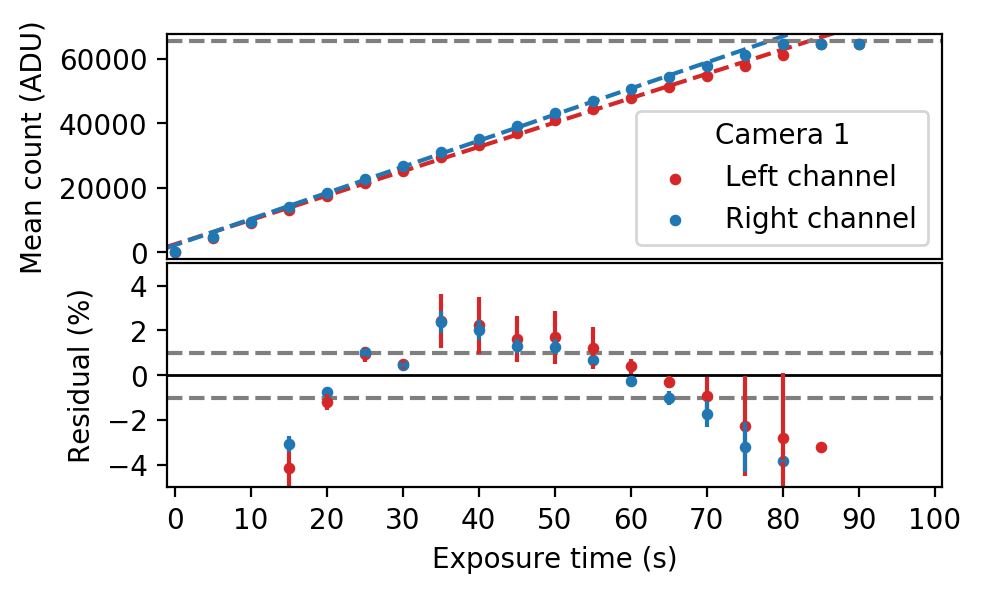
\includegraphics[width=\linewidth]{images/detectors/lin_1.png}
        \end{minipage}
        \begin{minipage}[t]{0.49\textwidth}\vspace{10pt}
            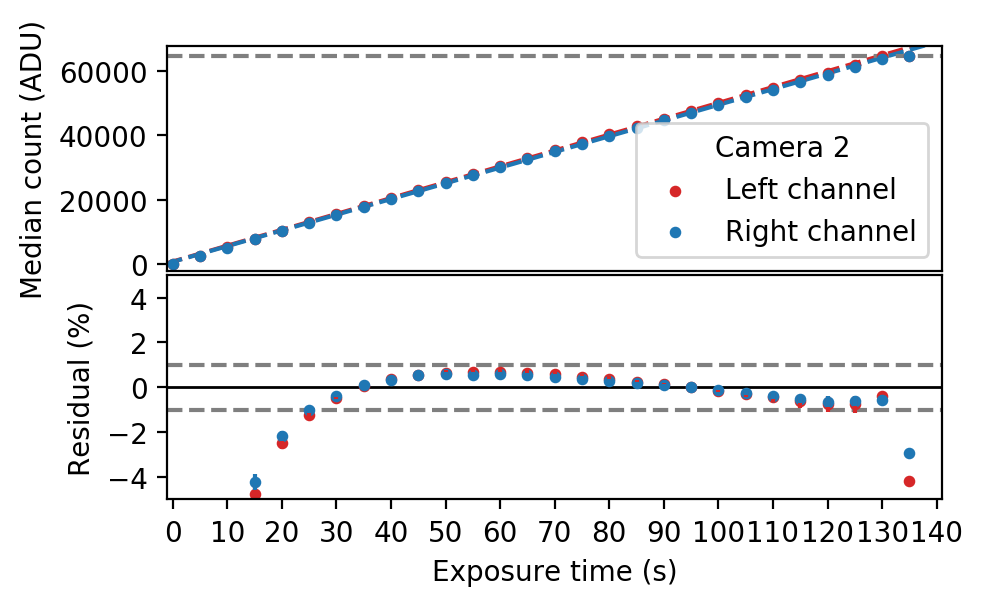
\includegraphics[width=\linewidth]{images/detectors/lin_2.png}
        \end{minipage}

        \begin{minipage}[t]{0.49\textwidth}\vspace{10pt}
            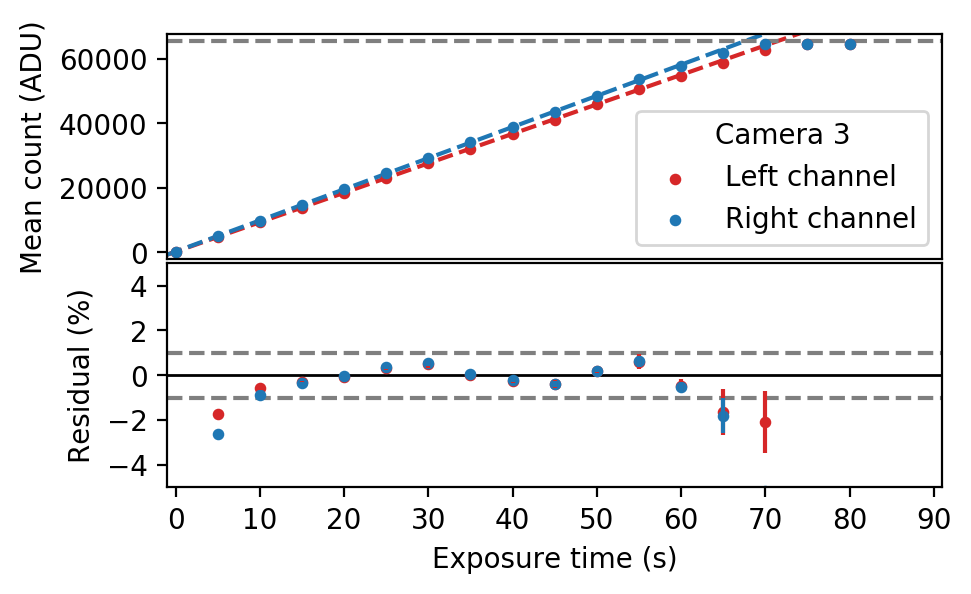
\includegraphics[width=\linewidth]{images/detectors/lin_3.png}
        \end{minipage}
        \begin{minipage}[t]{0.49\textwidth}\vspace{10pt}
            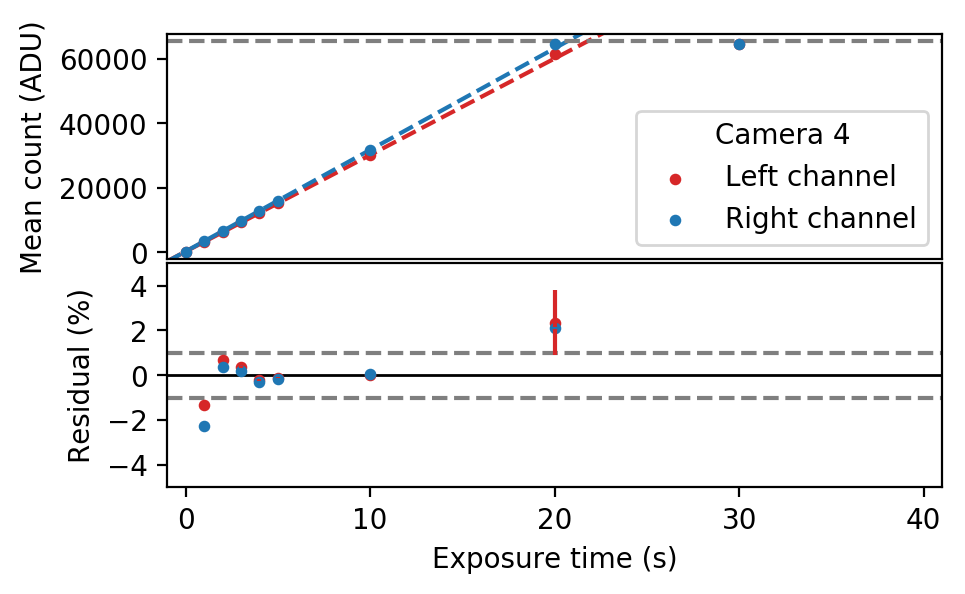
\includegraphics[width=\linewidth]{images/detectors/lin_4.png}
        \end{minipage}

        \begin{minipage}[t]{0.49\textwidth}\vspace{10pt}
            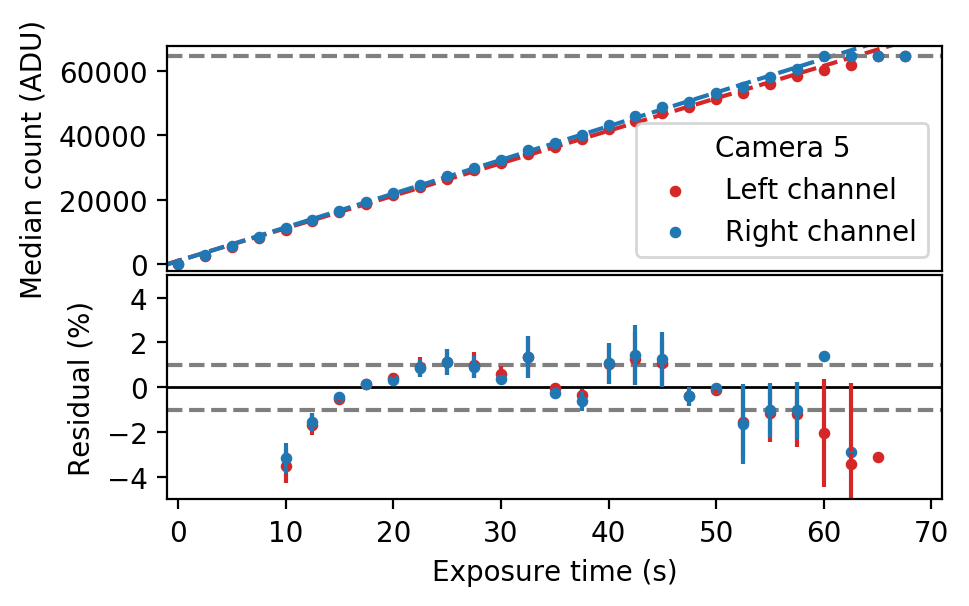
\includegraphics[width=\linewidth]{images/detectors/lin_5.png}
        \end{minipage}
        \begin{minipage}[t]{0.49\textwidth}\vspace{10pt}
            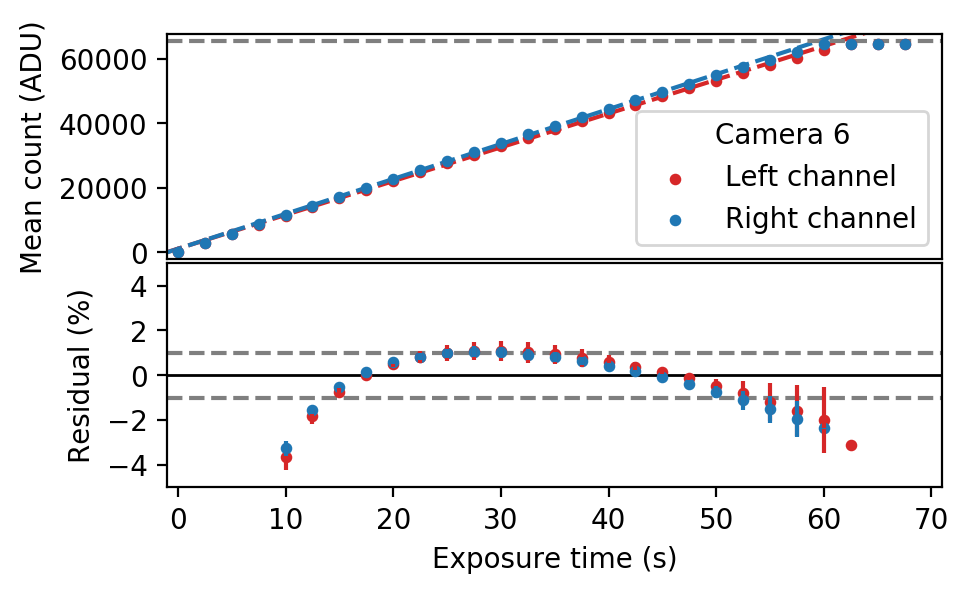
\includegraphics[width=\linewidth]{images/detectors/lin_6.png}
        \end{minipage}

        \begin{minipage}[t]{0.49\textwidth}\vspace{10pt}
            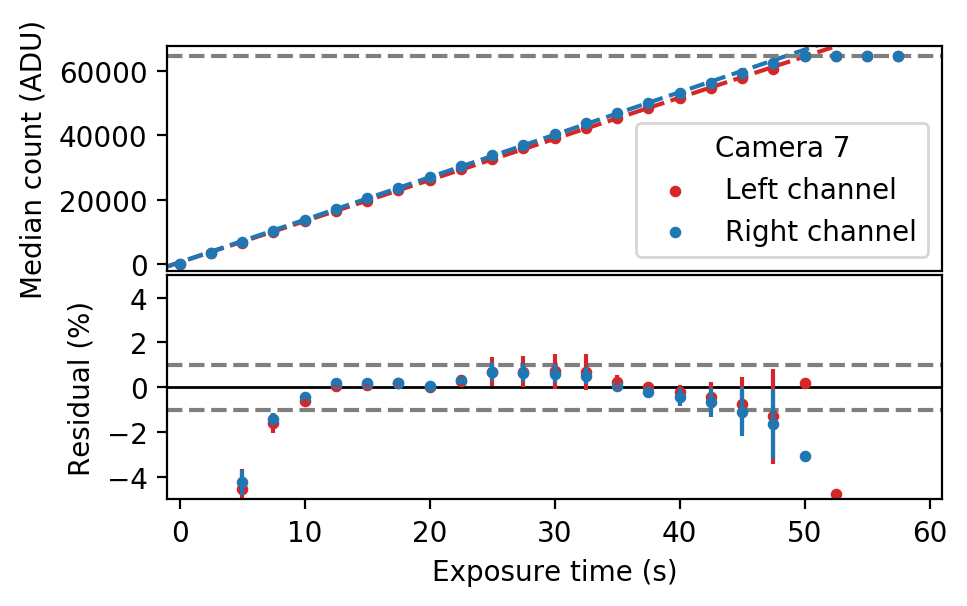
\includegraphics[width=\linewidth]{images/detectors/lin_7.png}
        \end{minipage}
        \begin{minipage}[t]{0.49\textwidth}\vspace{10pt}
            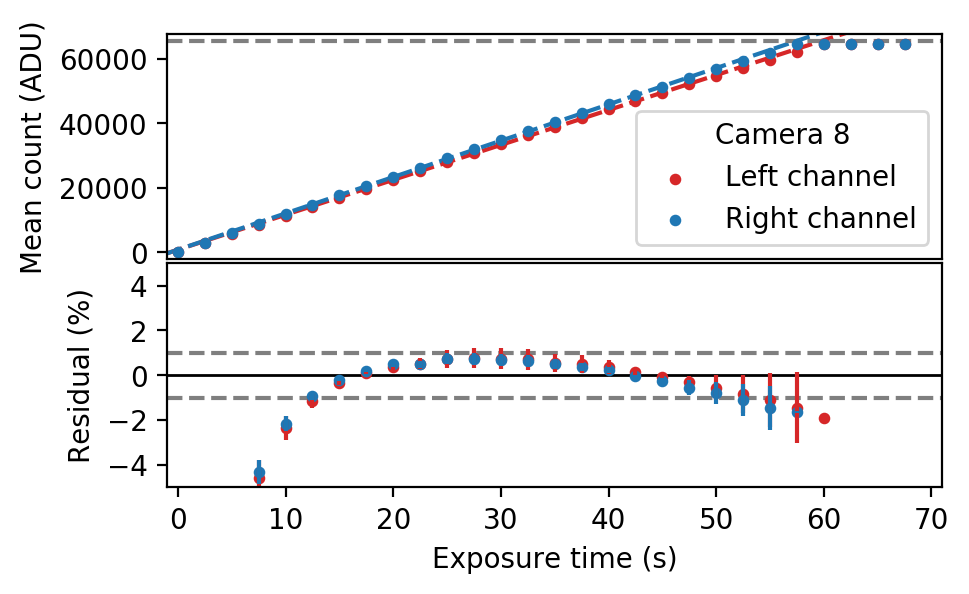
\includegraphics[width=\linewidth]{images/detectors/lin_8.png}
        \end{minipage}
    \end{center}
    \caption[Linearity plots]{
        Linearity plots for each camera.
    }\label{fig:lin}
\end{figure}

\clearpage

\end{colsection}

% ~~~~~~~~~~~~~~~~~~~~
\newpage
\subsection{Defects}
\label{sec:defects}
\begin{colsection}

There are several possible defects in CCD sensors \citep{CCDs}: hot pixels, which have atypically high dark currents, dead pixels, which produce zero counts, and trap pixels, which ``trap'' electrons and prevent read out from it and any pixels above it in the column. For targeted astronomical observations it is important to track any bad pixels, so whenever possible photons from the target object does not fall on any of them. GOTO's wide-field survey observations make this less of an issue, but the pipeline will track bad pixels and columns when calibrating images from each camera.

Single hot or dead pixels are not a major problem, as they can be removed by subtracting bias frames and flat fielding. If necessary the value of the bad pixel can be interpolated from the surrounding pixels. Trap pixels are more of an issue, as they take out the entire column behind them. For each camera a defect mask was made by taking the ratio of two flat images with different exposure times, making any bad pixels or columns easy to pick out by comparing to the surrounding pixels. And example of a trap pixel is shown in \aref{fig:itsatrap}. The positions of trap pixels for each camera are given in \aref{tab:traps}. The KAF-50100 chip specification gives an allowed limit of less than 20 column defects per device, which the GOTO cameras are well within.

\begin{table}[t]
    \begin{center}
        \begin{tabular}{c|ccc} %chktex 44
             & \multicolumn{2}{c}{Trap location} & Lost \\
             & x & y & \% \\
            \midrule
            Camera 1 & 7751 & 4361 & 30 \\
            Camera 2 & 1658 & ~172 & 97 \\ %chktex 39
            Camera 3 & 1224 & 1844 & 70 \\
                     & 5058 & 5185 & 17 \\
            Camera 4 & 5406 & 2607 & 58 \\
            Camera 5 & 6293 & 1416 & 77 \\
            Camera 6 & 5455 & 5036 & 19 \\
        \end{tabular}
        \hspace{0.5cm}
        \begin{tabular}{c|ccc} %chktex 44
            & \multicolumn{2}{c}{Trap location} & Lost \\
            & x & y & \% \\
            \midrule
            Camera 7 & 1344 & 3037 & 51 \\
                     & 2326 & 2495 & 60 \\
                     & 2610 & 5688 & ~9 \\ %chktex 39
                     & 7491 & 5120 & 18 \\
            Camera 8 & 1184 & 3043 & 51 \\
                     & 5659 & 2778 & 55 \\
            \multicolumn{4}{c}{} \\
        \end{tabular}
    \end{center}
    \caption[Locations of trap pixels]{
        Locations of trap pixels and fraction of the column lost for each camera.
    }\label{tab:traps}
\end{table}

\begin{figure}[p]
    \begin{center}
        \includegraphics[width=\textwidth]{images/detectors/defect_plot.pdf}
    \end{center}
    \caption[An example of a trap pixel]{
        A flat frame for Camera 1 showing an example of a trap pixel. The plot below of counts averaged in the y axis clearly shows the bad column, and the depth of the well beneath the field level is proportional to the height of the trap pixel in the column.
    }\label{fig:itsatrap}
\end{figure}

\clearpage

\end{colsection}

% ~~~~~~~~~~~~~~~~~~~~

\end{colsection}

% ########################################

\newpage
\section{System throughput}
\label{sec:throughput}
\begin{colsection}

% ~~~~~~~~~~~~~~~~~~~~

\begin{colsection}

Unfortunately, not every photon emitted by a target object will reach our cameras. Photons will be lost due to the finite transmittance of the telescope optics, and before that a certain fraction of light will be lost due to extension in the atmosphere. Understanding each element is required in order to produce a complete throughput model.

\end{colsection}

% ~~~~~~~~~~~~~~~~~~~~
\subsection{Optical elements}
\label{sec:optics}
\begin{colsection}

The GOTO unit telescopes are Wynne-Newtonian astrographs: fast (f/2.5) Newtonian telescopes with a \SI{40}{\centi\meter} primary mirror, a flat elliptical secondary (\SI{19}{\centi\metre} short axis) and a three-lens Wynne corrector between the secondary mirror and camera to focus light back onto the CCD detector. The full \gls{ota} design is shown in \aref{fig:ota}, and the five elements the light must pass through (the three corrector lenses, the filter in the filter wheel and the window in front of the detector) are shown in \aref{fig:wynne}. In order to correctly model the throughput each element needed to be considered in turn.

% ---------
\subsubsection{Mirrors}

The GOTO mirrors are made of coated aluminium, and were manufactured by Orion Optics\footnote{\url{https://www.orionoptics.co.uk/}}. Orion uses their own ``HiLux'' high reflectivity coating, and while individual reflectance curves were not available for the GOTO mirrors at the time this work was carried out Orion does provide a representative reflectance curve on their website (shown in \aref{fig:trans_ota}). As there are two mirrors this curve will be included twice in the final throughput model. Orion's website states that the difference in angle of incidence of the two mirrors is accounted for in the thickness of the coating applied, so otherwise the two mirrors can be treated as identical.

\newpage

\begin{figure}[p]
    \begin{center}
        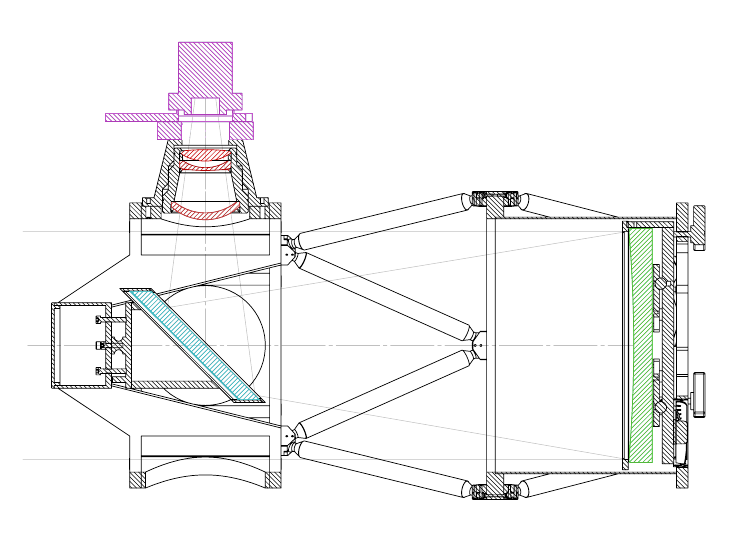
\includegraphics[width=0.7\textwidth]{images/throughput/OTA_optics.png}
    \end{center}
    \caption[GOTO optical telescope assembly]{
        The \gls{ota} design for one of the GOTO prototype unit telescopes. Light enters from the left, and the optical elements have been highlighted: the primary mirror in \textcolorbf{Green}{green}, the secondary mirror in \textcolorbf{BlueGreen}{blue}, the Wynne corrector lenses in \textcolorbf{Red}{red} and the FLI camera hardware (focuser, filter wheel and camera) in \textcolorbf{Purple}{purple}.
    }\label{fig:ota}
\end{figure}

\begin{figure}[p]
    \begin{center}
        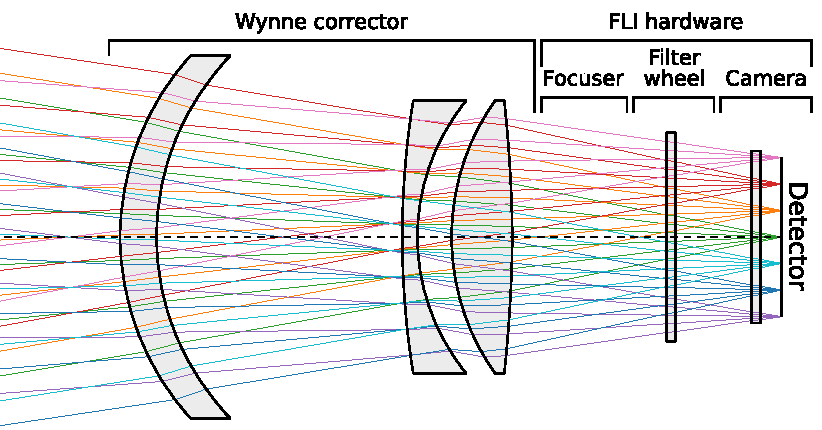
\includegraphics[width=0.7\textwidth]{images/throughput/wynne.pdf}
    \end{center}
    \caption[Ray tracing the corrector elements]{
        A ray trace showing the optical elements after the secondary mirror. From left-to-right light passes through the three Wynne corrector lenses, the focuser (which contains no optical elements), the filter in the filter wheel and the camera window before reaching the detector located in the focal plane.
    }\label{fig:wynne}
\end{figure}

\clearpage

% ---------
\subsubsection{Lenses}

\begin{table}[t]
    \begin{center}
        \begin{tabular}{c|cccc} %chktex 44
            Lens & Type     & Glass (manufacturer) & Diameter               & On-axis thickness \\
            \midrule
               1 & Crescent &    H-K9L (Schott)    & \SI{120}{\milli\meter} & \SI{12}{\milli\meter} \\
               2 & Crescent &    H-K9L (Schott)    & \SI{90}{\milli\meter}  & \SI{5}{\milli\meter} \\
               3 & Biconvex &  S-FPL53 (Ohara)     & \SI{90}{\milli\meter}  & \SI{20}{\milli\meter} \\
        \end{tabular}
    \end{center}
    \caption[Wynne corrector lens properties]{
        Properties of the three Wynne corrector lenses.
    }\label{tab:lenses}
\end{table}

Each Wynne corrector contains three lenses, as shown in \aref{fig:wynne}, and the physical details of each lens are given in \aref{tab:lenses}. No complete transmission data was available, so a model throughput curve was created.

Both the reflectivity of the front surface and the internal transmittance of the lens glass needs to be considered. Each lens was coated with an anti-reflection coating, the profile of which was included in the GOTO optical report. Transmittance curves for each lens were not available, however the glass types were included in the report and are given in \aref{tab:lenses}. Transmittance data provided by the manufacturers was retrieved from the online Refractive Index Database\footnote{\url{https://refractiveindex.info/}}. For simplicity each lens was modelled as having a constant thickness, using their on-axis thickness. As shown in \aref{fig:wynne} this is true for lens 1 but will typically underestimate the thickness of lens 2 and overestimate the thickness of lens 3. However the thickness of glass each light path travels through should be the same, and as there is very little difference between the two types of glass the overall throughput will be approximately the same.

Throughput curves for the anti-reflection coating and the three lenses are shown in \aref{fig:trans_lenses}, along with the total throughput found by multiplying the contribution from the glass and coating for each lens.

\newpage

\begin{figure}[t]
    \begin{center}
        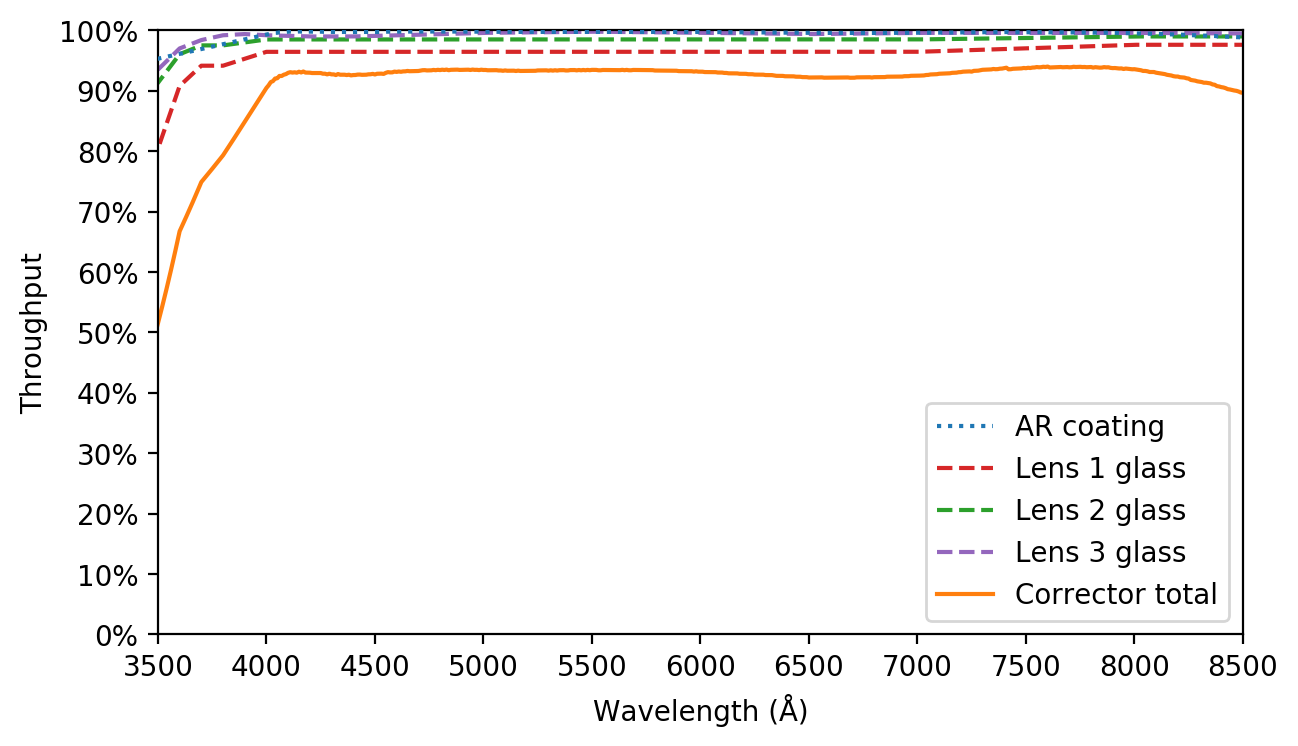
\includegraphics[width=\textwidth]{images/throughput/trans_lenses.png}
    \end{center}
    \caption[Wynne corrector transmission curve]{
        Transmission curve for the Wynne corrector, comprised of the three lenses each with an anti-reflection (AR) coating.
    }\label{fig:trans_lenses}
\end{figure}

% ---------
\subsubsection{Filters}

The filter transmittance is included in their bandpass profiles, described below in \aref{sec:filters}. At this stage we will consider the \gls{ota} with no filter in place.

% ---------
\subsubsection{Camera window}

Finally, before reaching the detector light must pass through a glass window in the camera which protects the CCD sensor. The window is made of F116 glass, and a transmission profile was provided by FLI.\@ This is shown in \aref{fig:trans_ota}.

\newpage

% ---------
\subsubsection{Combined OTA throughput}

The combined throughput for the whole unfiltered OTA is shown in \aref{fig:trans_ota}. This was constructed by multiplying through the transmission curves for the two mirrors, the corrector and the camera window. In the 4000--\SI{7000}{\angstrom} visible region used by GOTO the throughput is typically 60\% or above, although all the elements have a sharp cut-off towards the UV at low wavelengths.

\begin{figure}[t]
    \begin{center}
        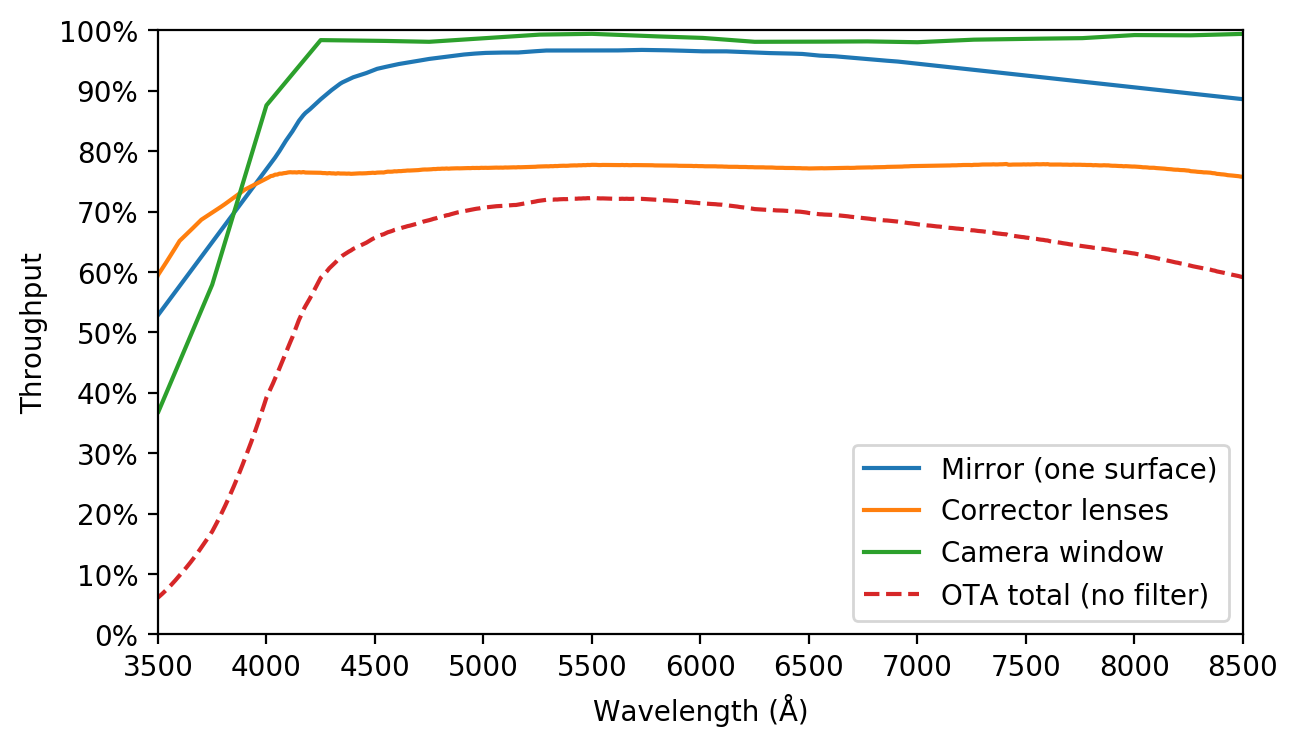
\includegraphics[width=\textwidth]{images/throughput/trans_ota.png}
    \end{center}
    \caption[Combined OTA transmission curve]{
        Transmission curve for the unfiltered OTA, including two mirrors, the corrector lenses and the camera window.
    }\label{fig:trans_ota}
\end{figure}

\end{colsection}

% ~~~~~~~~~~~~~~~~~~~~
\newpage
\subsection{Filters}
\label{sec:filters}
\begin{colsection}

\begin{figure}[t]
    \begin{center}
        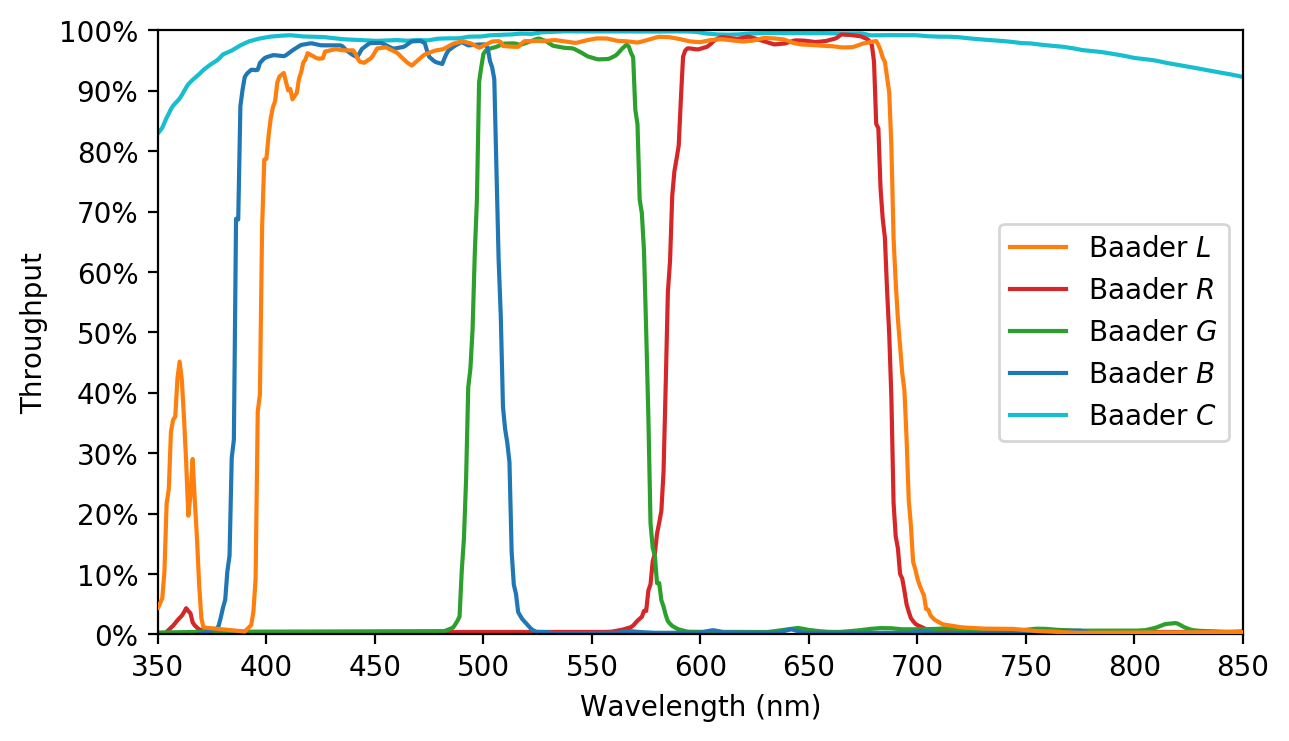
\includegraphics[width=\textwidth]{images/throughput/trans_filters.png}
    \end{center}
    \caption[Baader filter transmission curves]{
        Transmission curves for the Baader \textit{LRGBC} filter set used by GOTO.\
    }\label{fig:filters}
\end{figure}

Each GOTO unit telescope has a five-slot CFW9--5 filter wheel from FLI.\@ Each contains a set of \SI{65}{\milli\metre} square filters from Baader Planetarium\footnote{\url{https://www.baader-planetarium.com/}}: three coloured filters (\textit{R}, \textit{G}, \textit{B}), one wide ``luminance'' filter (\textit{L}) covering the whole visible range, and a clear glass filter ({\textit{C}}). Transmission curves for each filter are shown in \aref{fig:filters}. Each filter has a high throughput and steep cut-offs outside of the desired bandpasses. For the coloured filters the cut-offs were chosen so the [O\textsc{iii}] $\lambda 5007$ emission line falls within the overlap of the \textit{B} and \textit{G} filters and the region around \SI{5800}{\angstrom}, which contains emission lines from Mercury and Sodium vapour lamps, is excluded by the gap between the \textit{G} and \textit{R} filters.

The clear filter is never used for scientific observations, so from now on only the \textit{LRGB} filters are considered. Most of GOTO observations are taken using the \textit{L} filter, because it would currently take too long to survey in multiple colours. However the \textit{RBG} filters have been used for targeted observations and manual follow-up images.

\begin{table}[t]
    \begin{center}
        \begin{tabular}{c|cccc} %chktex 44
            Filter            & Central wavelength                          & Bandwidth            \\
             & ($\lambda_\text{eff}$, \SI{}{\angstrom}) & ($\Delta\lambda$, \SI{}{\angstrom}) \\
            \midrule
            Baader \textit{L} & 5355 & 2942 \\
            Baader \textit{R} & 6573 &  979 \\
            Baader \textit{G} & 5373 &  813 \\
            Baader \textit{B} & 4509 & 1188 \\
        \end{tabular}
    \end{center}
    \caption[Baader filter properties]{
        Properties of the Baader \textit{LRGB} filters.
    }\label{tab:filters}
\end{table}

Properties of the four \textit{LRGB} filters are given in \aref{tab:filters}. The effective wavelength $\lambda_\text{eff}$ given is the pivot wavelength as defined in \citet{HST_calibration} for HST filters

\begin{equation}
    \lambda_\text{eff}^2 = \frac{\int T\lambda \, d\lambda}{\int T/\lambda \, d\lambda},
    \label{eq:pivot_wavelength}
\end{equation}

where $T$ is the transmission integrated over all wavelengths $\lambda$. The effective bandwidth $\Delta\lambda$ is defined as the width of a rectangle that has a height of the maximum transmission (1) and the same area as the area under the filter transmission curve, i.e.

\begin{equation}
    \Delta\lambda = \int T d\lambda.
    \label{eq:bandwidth}
\end{equation}

GOTO uses the Baader filters primarily based on cost, as each complete mount would require 8 filter sets. The Baader filters were designed for amateur astronomers and astro-photographers and are less common for scientific instruments than other sets; such as the \textit{u'g'r'i'z'} set used by the Sloan Digital Sky Survey \citep{Sloan_filters}, or the traditional Johnson-Cousins \textit{UBVRI} set redefined in \citet{Bessell_filters}. A comparison of the transmission curves are shown in \aref{fig:filter_comparison1} for Sloan and \aref{fig:filter_comparison2} for Bessell. As can be seen the Baader \textit{L} filter approximately covers the extent of the Sloan \textit{g'} and \textit{r'}, with the \textit{B} and \textit{G} filters covering \textit{g'} and \textit{R} roughly matching \textit{r'}. Colour terms to compare GOTO \textit{RBG} observations with others using the Sloan \textit{g'} and \textit{r'} filters were calculated in \citet{Phaethon}.

\newpage

\begin{figure}[t]
    \begin{center}
        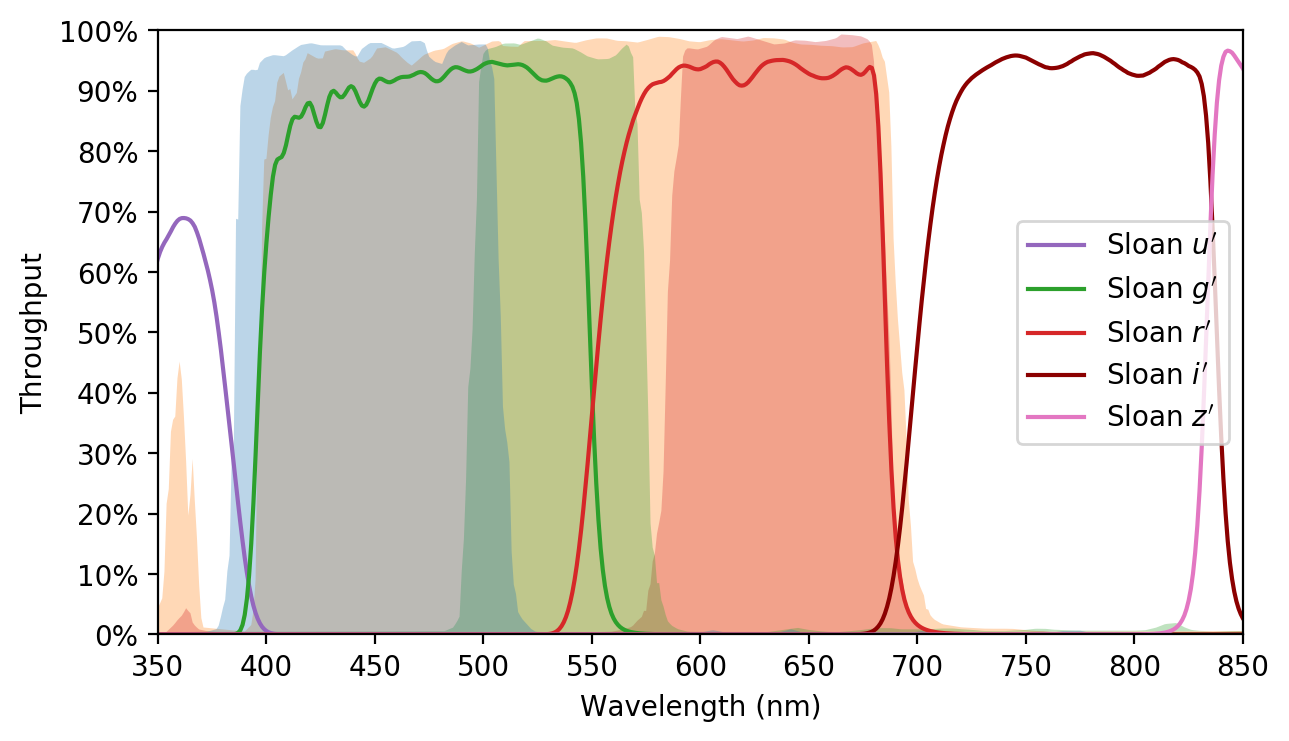
\includegraphics[width=\textwidth]{images/throughput/filt_comp1.png}
    \end{center}
    \caption[Comparison of Baader and Sloan filters]{
        A comparison of the Baader \textit{LRGB} filters to the Sloan \textit{u'g'r'i'z'} set.
    }\label{fig:filter_comparison1}
\end{figure}

\begin{figure}[t]
    \begin{center}
        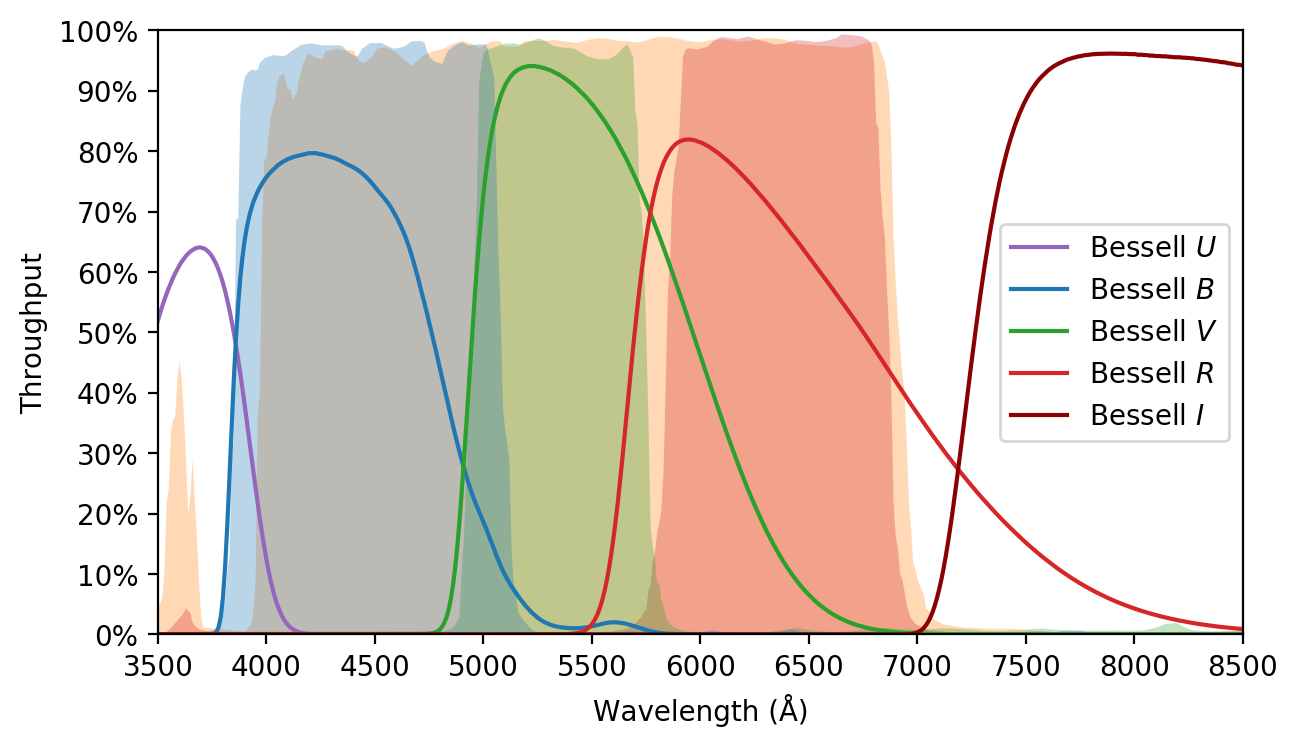
\includegraphics[width=\textwidth]{images/throughput/filt_comp2.png}
    \end{center}
    \caption[Comparison of Baader and Bessell filters]{
        A comparison of the Baader \textit{LRGB} filters to the Bessell \textit{UBVRI} set.
    }\label{fig:filter_comparison2}
\end{figure}

\clearpage

\end{colsection}

% ~~~~~~~~~~~~~~~~~~~~
\newpage
\subsection{Atmospheric extinction}
\label{sec:atmosphere}
\begin{colsection}

In order to fully model light from an astronomical source through to the CCD detector the absorption of light by the Earth's atmosphere must also be considered. The atmosphere is close to transparent over most of the visible region, however losses due to Rayleigh scattering begin to dominate closer to the UV \citep{atmosphere}.

The amount of light lost due to absorption and scattering in the atmosphere will depend on the altitude of the source, as light from sources closer to the horizon will pass through more atmosphere. The transmission of the atmosphere above La Palma has been measured as a function of airmass in \citet{tn31}, and is shown in \aref{fig:trans_atm}.

\begin{figure}[t]
    \begin{center}
        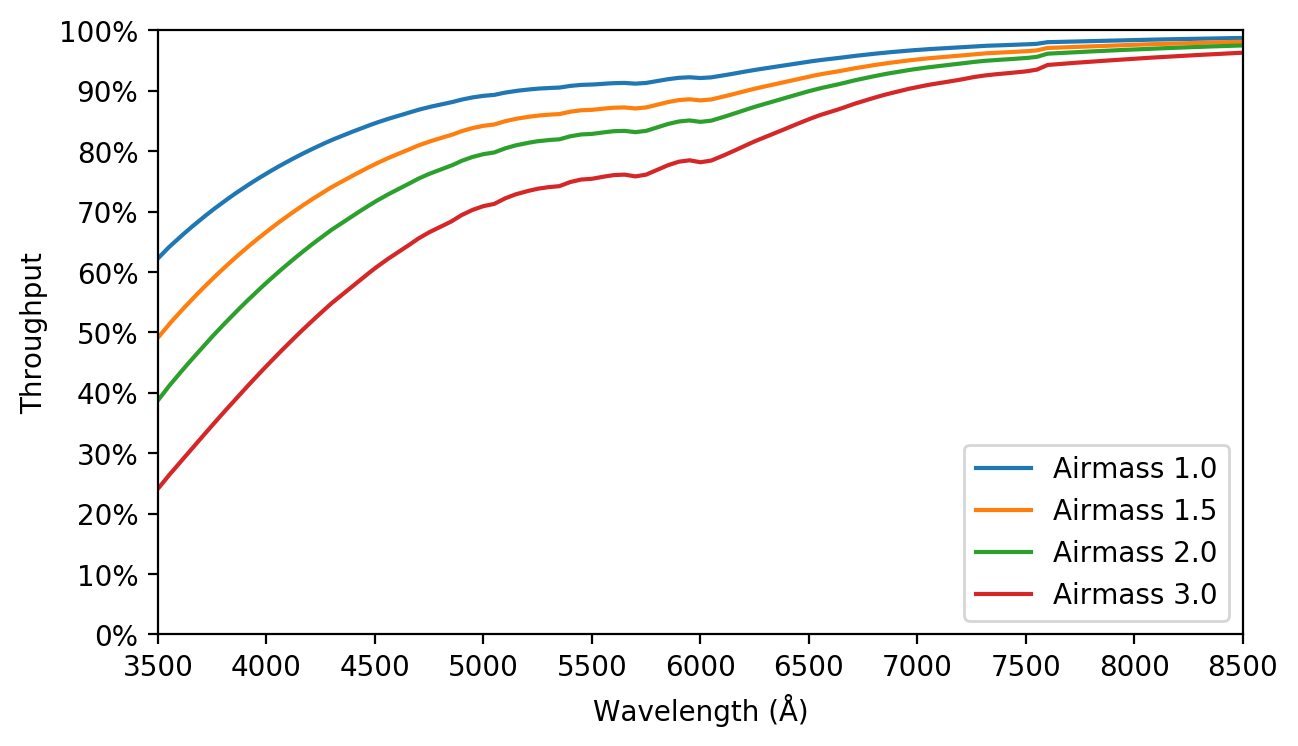
\includegraphics[width=\textwidth]{images/throughput/trans_atm.png}
    \end{center}
    \caption[Atmospheric transmission curve]{
        Transmission curve for the atmosphere at several airmasses.
    }\label{fig:trans_atm}
\end{figure}

\end{colsection}

% ~~~~~~~~~~~~~~~~~~~~
\newpage
\subsection{Quantum efficiency}
\label{sec:qe}
\begin{colsection}

\begin{figure}[t]
    \begin{center}
        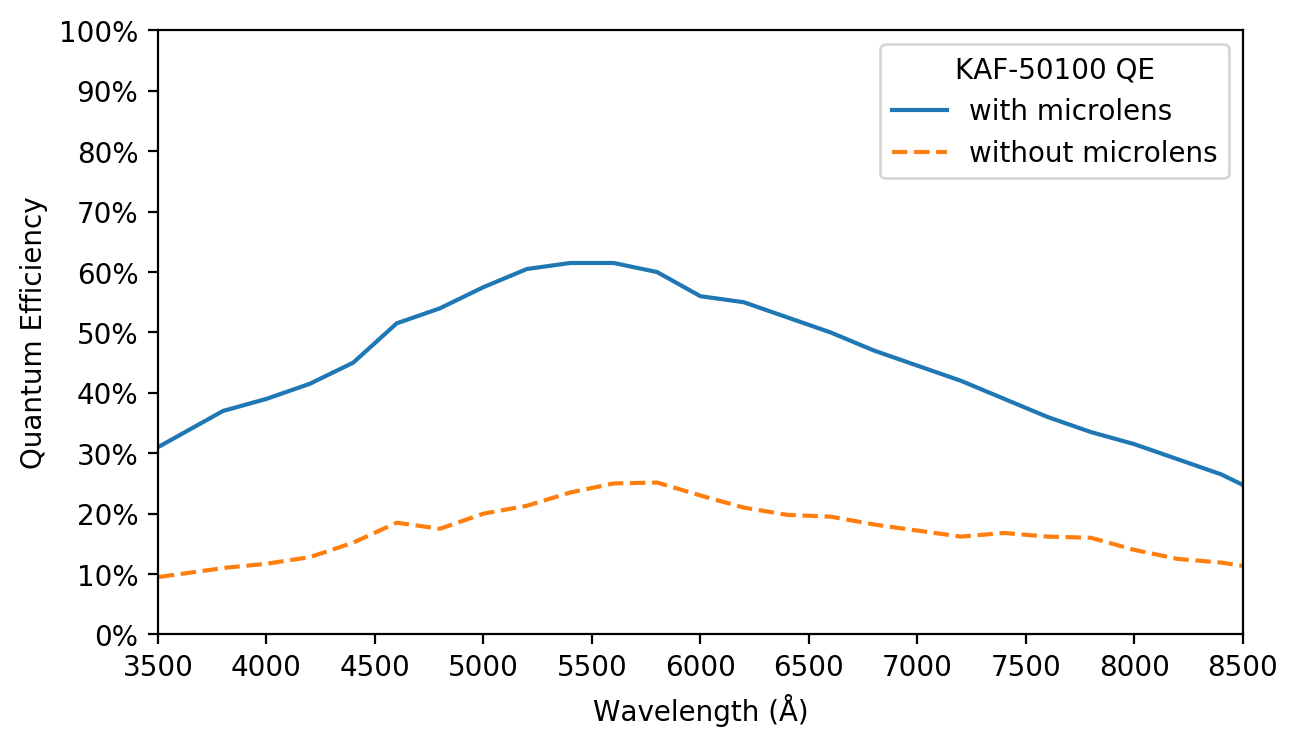
\includegraphics[width=\textwidth]{images/throughput/qe.png}
    \end{center}
    \caption[MicroLine quantum efficiency curve]{
        Quantum efficiency curve for the GOTO MicroLine cameras.
    }\label{fig:qe}
\end{figure}

Once photons pass through the atmosphere and the telescope they are focused onto the CCD, where they interact with the photosensitive layer and produce electric charge carriers which are recorded by the detector \citep{CCDs}. The conversion from photons to electrons is measured by the \gls{qe} of the CCD and is dependent on wavelength: short-wavelength photons will be absorbed before reaching the photosensitive layer, while long wavelength photons will not have enough energy to create free electrons from the silicon. The QE curve for the front-illuminated KAF-50100 CCDs within the GOTO MicroLine cameras was provided by FLI, and is shown in \aref{fig:qe}. CCDs that are back-side illuminated have improved QE as each photon passes through fewer layers and therefore has less chance of being absorbed, however these are more complicated and expensive to build. The quantum efficiency of a CCD can also change as a function of temperature, but this is negligible in the visible portion of the spectrum. % The QE peaks at 60\% at \SI{5500}{\angstrom} and falls below 30\% outside of the visible region.

\end{colsection}

% ~~~~~~~~~~~~~~~~~~~~
\newpage
\subsection{Total throughput}
\label{sec:total_throughput}
\begin{colsection}

The complete GOTO throughput is a combination of all of the above elements. Each source profile was linearly extrapolated to fit the same wavelength range (3500--\SI{8500}{\angstrom}) and multiplied together to produce the complete throughput model, shown in \aref{fig:throughput}. As the quantum efficiency is included the throughput describes the conversion between photons entering the atmosphere to electrons detected in the CCD, and using with the gain values given in \aref{tab:ptc} the full conversion between source photons and output counts can be made. The mean throughput in each filter can be found by dividing the filled areas in \aref{fig:throughput} by the area of the filter bandpass, these are given in electrons per photon in \aref{tab:throughput_zeropoint} in the next section.

\begin{figure}[t]
    \begin{center}
        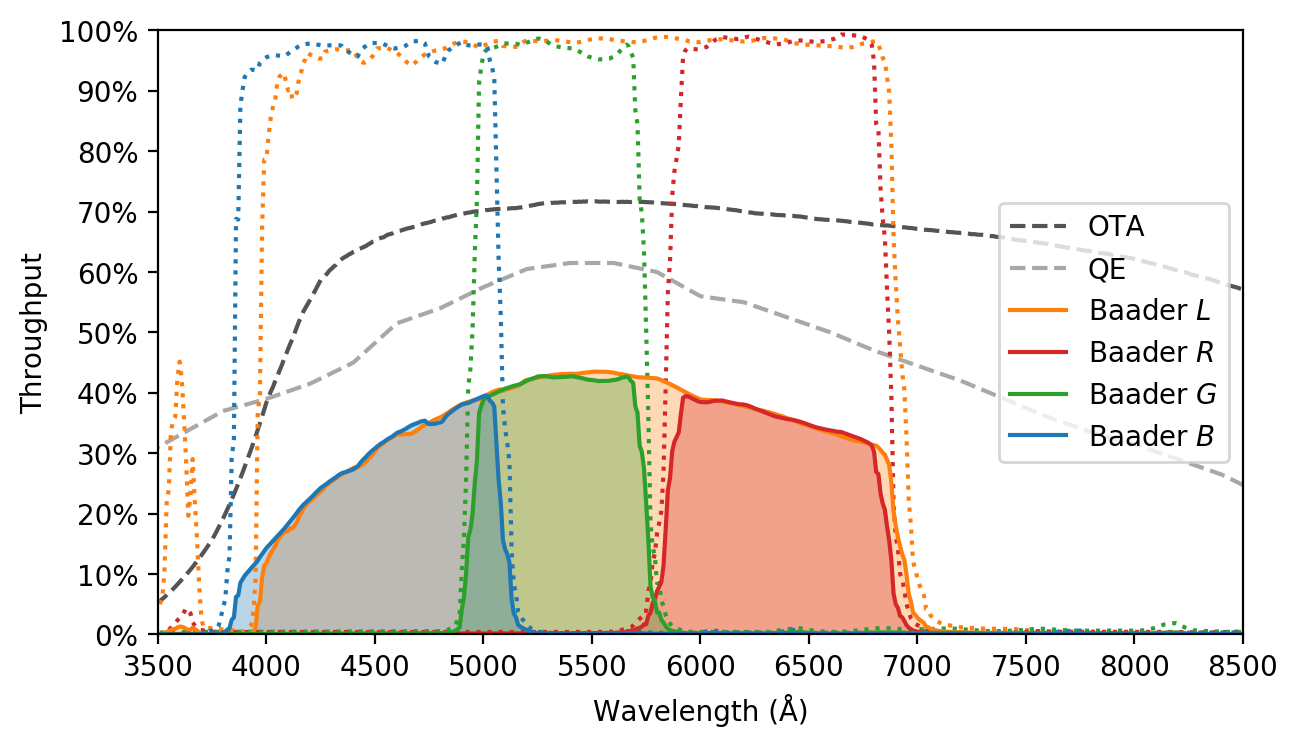
\includegraphics[width=\textwidth]{images/throughput/throughput.png}
    \end{center}
    \caption[Complete throughput model for the GOTO filters]{
        The complete GOTO throughput model for the Baader \textit{LRGB} filters (bandpasses from \aref{fig:filters}). Other contributions are from atmospheric extinction (from \aref{fig:trans_atm}, here assuming a source at zenith), throughput of the OTA elements (from \aref{fig:trans_ota}) and the quantum efficiency of the cameras (from \aref{fig:qe}).
    }\label{fig:throughput}
\end{figure}

\end{colsection}

% ~~~~~~~~~~~~~~~~~~~~

\end{colsection}

% ########################################

\newpage
\section{Photometric modelling}
\label{sec:photometry}
\begin{colsection}

% ~~~~~~~~~~~~~~~~~~~~

\begin{colsection}

Using the throughput model created in the previous section it is possible to simulate photometric observations with GOTO before the telescope was even commissioned. This section applies the theoretical model to two important photometric properties: the magnitude zeropoint, the correction required to convert between instrumental and ``real'' magnitude values, and the limiting magnitude, the brightest magnitude a source can bbe to still produce a noticeable signal above a given noise threshold. These theoretical values are then compared to values calculated from real GOTO observations in order to test the validity of the model and check that the hardware is performing to specification.

\end{colsection}

% ~~~~~~~~~~~~~~~~~~~~
\subsection{Magnitude zeropoints}
\label{sec:zeropoints}
\begin{colsection}

The output flux of a source, $F$, is related to its magnitude, $m$, by
%
\begin{equation}
    m = -2.5 \log_{10}(F).
    \label{eq:apparent_magnitude}
\end{equation}
%
In practice magnitudes are usually measured relative to a particular reference star using
%
\begin{equation}
    m - m_\text{ref} = -2.5 \log_{10}\left(\frac{F}{F_\text{ref}}\right),
    \label{eq:magnitude_ref}
\end{equation}
%
which requires a reference star of known magnitude $m_\text{ref}$ and flux $F_\text{ref}$. By definition, a star with a magnitude of zero should produce a flux of one photon per second; traditionally Vega is used as a reference star as it has a magnitude of very close to 0.

The instrumental magnitude measured from an image is related to the number of photo-electrons recorded, $N$, using the same magnitude definition
%
\begin{equation}
    \begin{split}
        m_\text{ins} & = -2.5 \log_{10}(N/t) \\
                     & = -2.5 \log_{10}(gS/t),
    \end{split}
    \label{eq:ins_mag}
\end{equation}
%
where $t$ is the exposure time and \aref{eq:gain} was used to convert the number of electrons to counts, $S$, using the gain $g$. This is assuming the image has already been calibrated (corrected for bias, dark current and flat-fielded), the number of counts within a given aperture around the object has been measured, and a background level of counts has also been subtracted; in this case $S$ should, ideally, only include counts from the source object.

The number of photo-electrons recorded per second $N/t$ from a given source should be proportional to the source output flux $F$ (assuming the camera has a low non-linearity, see \aref{sec:lin}). Relating the two through a constant $\kappa$ \aref{eq:ins_mag} becomes
%
\begin{equation}
    \begin{split}
        m_\text{ins} & = -2.5 \log_{10}\left(\kappa F\right) \\
                     & = -2.5 \log_{10}\left(F\right) - m_\text{ZP}    \\
                     & = m - m_\text{ZP},
    \end{split}
    \label{eq:ins_mag2}
\end{equation}
%
where constant $m_\text{ZP}$ is defined as the instrumental \emph{zeropoint}. The zeropoint is so called because observing an object with a true magnitude equal to the zeropoint ($m = m_\text{ZP}$) will produce an instrumental magnitude of 0, which corresponds to one count per second in the image. Each telescope and filter combination will have a unique zeropoint, and once determined it can be used to convert instrumental magnitudes measured using that telescope to the source magnitude using
%
\begin{equation}
    m = m_\text{ins} + m_\text{ZP}.
    \label{eq:zp}
\end{equation}
%
Therefore, were it possible to observe a star with $m=0$ (without immediately saturating the telescope) and get a measured count rate the zeropoint can be calculated simply as
%
\begin{equation}
    \begin{split}
        m_\text{ZP} & = 0 - m_\text{ins} \\
                    & = 2.5 \log_{10}(N/t).
    \end{split}
    \label{eq:zp2}
\end{equation}

\end{colsection}

% ~~~~~~~~~~~~~~~~~~~~
\newpage
\subsection{Calculating theoretical zeropoints}
\label{sec:model_zeropoints}
\begin{colsection}

Consider taking an observation of a zero magnitude star, such as Vega. For this star $m=0$, and so from \aref{eq:zp} the instrumental magnitude will be equal to the negative zeropoint. In the AB magnitude system a zero magnitude star has a fixed flux density $F_\nu = $ \SI{3631}{\jansky} \citep{Sloan_filters}. Therefore passing that flux through the throughput model for each filter created in \aref{sec:throughput} will produce a predicted signal in photo-electrons which can be used to calculate an expected zeropoint.

First the zero-magnitude flux density needs to be converted into a flux in photons. \SI{3631}{\jansky} is equal to \SI{3.631e-20}{\erg\per\second\per\centi\metre\squared\per\hertz}. To convert from $F_\nu$ to photon flux $F_\lambda$ this needs to be multiplied by a factor of $c/\lambda_c^2$, where $c$ is the speed of light and $\lambda_c$ is the wavelength of the photon, in this case the central wavelength of the filter in question\footnote{The $c/\lambda_c^2$ conversion factor comes from differentiating the relationship $\nu = c/\lambda$}. This will then give a flux in Joules, but to convert to a photon count it needs to be divided by the energy of each photon $E_\lambda$ given by
%
\begin{equation}
    \begin{split}
        E_\lambda = \frac{hc}{\lambda_c},
    \end{split}
    \label{eq:photon_energy}
\end{equation}
%
where $h$ is Plank's constant. Again at this stage it is assumed that all the photons have the central wavelength of the filter. Therefore the expected flux in photons is given by
%
\begin{equation}
    \begin{split}
        F_\lambda = 1.51 \times 10^{26}/\lambda_c~\si{\photon\per\second\per\centi\metre\squared\per\angstrom}
    \end{split}
    \label{eq:zero-mag_photons}
\end{equation}
%
where $\lambda_c$ is given in Angstroms. This is still over a particular range of wavelengths and per unit area, so needs to be multiplied by the filter bandwidth and the collecting area of the telescope. Each of GOTO's unit telescopes has a \SI{40}{\centi\metre} diameter primary mirror, however not all of this is available to collect photons due to the shadow of the spider mechanism holding the secondary mirror. Assuming this blocks 10\% of the light gives an effective collecting area of \SI{1131}{\centi\metre\squared}. Using this and the filter properties given in \aref{tab:filters} the expected signal in photons per second can be calculated for each filter, these values are given in \aref{tab:throughput_zeropoint}. Multiplying these by the throughput value calculated for each filter gives the expected photo-electron count per second (note this assumes the target star is at airmass 1, otherwise the throughput would decrease as discussed in \aref{sec:atmosphere}). Finally, converting these counts into magnitudes gives the instrumental magnitude, and using \aref{eq:zp2} with $m=0$ gives the theoretical zeropoint.

\begin{table}[t]
    \begin{center}
        \begin{tabular}{c|c|cc|c} %chktex 44
                   & Mean           & \multicolumn{2}{c|}{Zero-magnitude star} & \\
            Filter & Throughput     & Signal     & Count     & Zeropoint \\
                   & (\elec/photon) & (photon/s) & (\elec/s) & (mag) \\
            \midrule
            Baader \textit{L} & 0.3220 & \num{3.41e9} & \num{1.10e9} & 22.60 \\
            Baader \textit{R} & 0.3616 & \num{9.24e8} & \num{3.34e8} & 21.31 \\
            Baader \textit{G} & 0.3854 & \num{9.38e8} & \num{3.62e8} & 21.40 \\
            Baader \textit{B} & 0.2519 & \num{1.63e9} & \num{4.12e8} & 21.54 \\
        \end{tabular}
    \end{center}
    \caption[Throughputs and zeropoints for each of the GOTO filters]{
        Calculated throughputs for each of the GOTO filters, along with expected signals from a zero-magnitude star and predicted zeropoint.
    }\label{tab:throughput_zeropoint}
\end{table}

This method produces reasonable results, but is only approximating the filter bandpasses. A more robust model was created using the \pkg{pysynphot} (Python Synthetic Photometry) module\footnote{\url{https://pysynphot.readthedocs.io/}}, which is based the IRAF \pkg{SYNPHOT} package. Each of the throughput elements described in \aref{sec:throughput} were imported to create bandpasses for each filter, and observations were simulated of a flat spectrum of \SI{3631}{\jansky} (0 mag in the AB system) and the built-in Vega spectrum (0 mag in the Vega system) by convolving the spectra with the bandpasses. The resulting observation spectra are shown in \aref{fig:pysynphot} for both cases; the area under each curve gives the predicted signal. These counts and derived zeropoints are given in \aref{tab:pysynphot_zeropoints}. The AB counts and zeropoints are all lower than the previous values. The difference between the two systems is visible as the AB spectrum giving more counts in the red filter while the Vega spectrum is higher in the blue.

\newpage

\begin{figure}[p]
    \begin{center}
        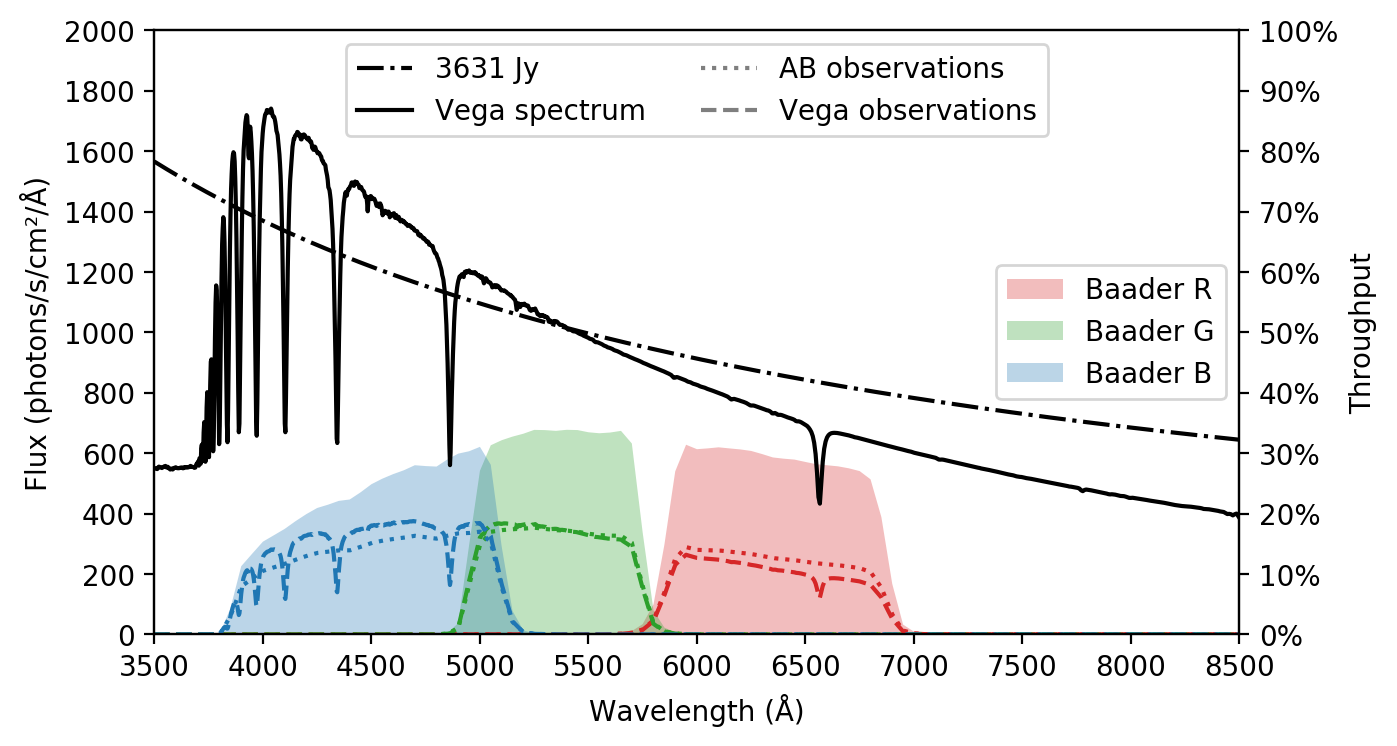
\includegraphics[width=\textwidth]{images/throughput/synphot.png}
    \end{center}
    \caption[Simulating photometric observations using pysynphot]{
        Simulating photometric observations in the GOTO filters using pysynphot. The filled coloured areas show the throughputs in the \textit{RGB} filters from \aref{fig:throughput}. The coloured dotted lines show the throughputs convolved with a flat \SI{3631}{\jansky} spectrum (dot-dashed black line), while the dashed lines show the throughputs convolved with the model Vega spectrum (solid black line). The same process was repeated for the \textit{L} filter (not shown for clarity).
    }\label{fig:pysynphot}
\end{figure}

\begin{table}[p]
    \begin{center}
        \begin{tabular}{c|cc|cc} %chktex 44
                   & \multicolumn{2}{c|}{AB system} & \multicolumn{2}{c}{Vega system}\\
            Filter & Signal    & Zeropoint & Signal    & Zeropoint\\
                   & (\elec/s) & (mag)     & (\elec/s) & (mag) \\
            \midrule
            Baader \textit{L} & \num{9.70e8} & 22.47 & \num{9.56e8} & 22.45 \\
            Baader \textit{R} & \num{2.96e8} & 21.18 & \num{2.51e8} & 21.00 \\
            Baader \textit{G} & \num{3.07e8} & 21.22 & \num{3.11e8} & 21.23 \\
            Baader \textit{B} & \num{3.98e8} & 21.50 & \num{4.38e8} & 21.60 \\
        \end{tabular}
    \end{center}
    \caption[Zeropoints in the AB and Vega systems calculated using pysynphot]{
        Zeropoints in the AB and Vega systems calculated using pysynphot.
    }\label{tab:pysynphot_zeropoints}
\end{table}

\clearpage

\end{colsection}

% ~~~~~~~~~~~~~~~~~~~~

\newpage
\subsection{Limiting magnitude}
\label{sec:lim_mag}
\begin{colsection}

Using the camera parameters determined in \aref{sec:detectors}, the throughput model created in \aref{sec:throughput} and the zeropoints calculated in \aref{sec:model_zeropoints} a complete photometric model of the GOTO telescopes can be created. One use of this is to predict the system limiting magnitude for a target signal-to-noise ratio.

% ---------
\subsubsection{Signal-to-noise}

The common sources of noise in CCDs are discussed in \aref{sec:noise}. Discounting the bias level and fixed-pattern noise, both properties of the camera which are easy to remove, the major sources of noise in an image will be the dark current and read-out noise. In addition, when taking on-sky images there will be a certain contamination level from background light. Accounting for these the total noise in the image is given by
%
\begin{equation}
    \sigma_\text{Total} = \sqrt{N + N_\text{BG} + D + R^2},
    \label{eq:total_noise}
\end{equation}
%
where $N$ is the electron signal from the source object, $N_\text{BG}$ is the additional signal from the background, $D$ is the dark current signal and $R$ is the read-out noise. Noise is usually quantified as a fraction of the target signal $N$, known as the signal-to-noise ratio:
%
\begin{equation}
    \text{SNR} = \frac{N}{\sigma_\text{Total}} = \frac{N}{\sqrt{N + N_\text{BG} + D + R^2}}.
    \label{eq:snr}
\end{equation}

For good science-quality observations a signal-to-noise value of 5 or more is required, also known as a $5\sigma$ detection (as the signal will be more than 5 times the noise).

\newpage

% ---------
\subsubsection{Background noise}

\begin{figure}[t]
    \begin{center}
        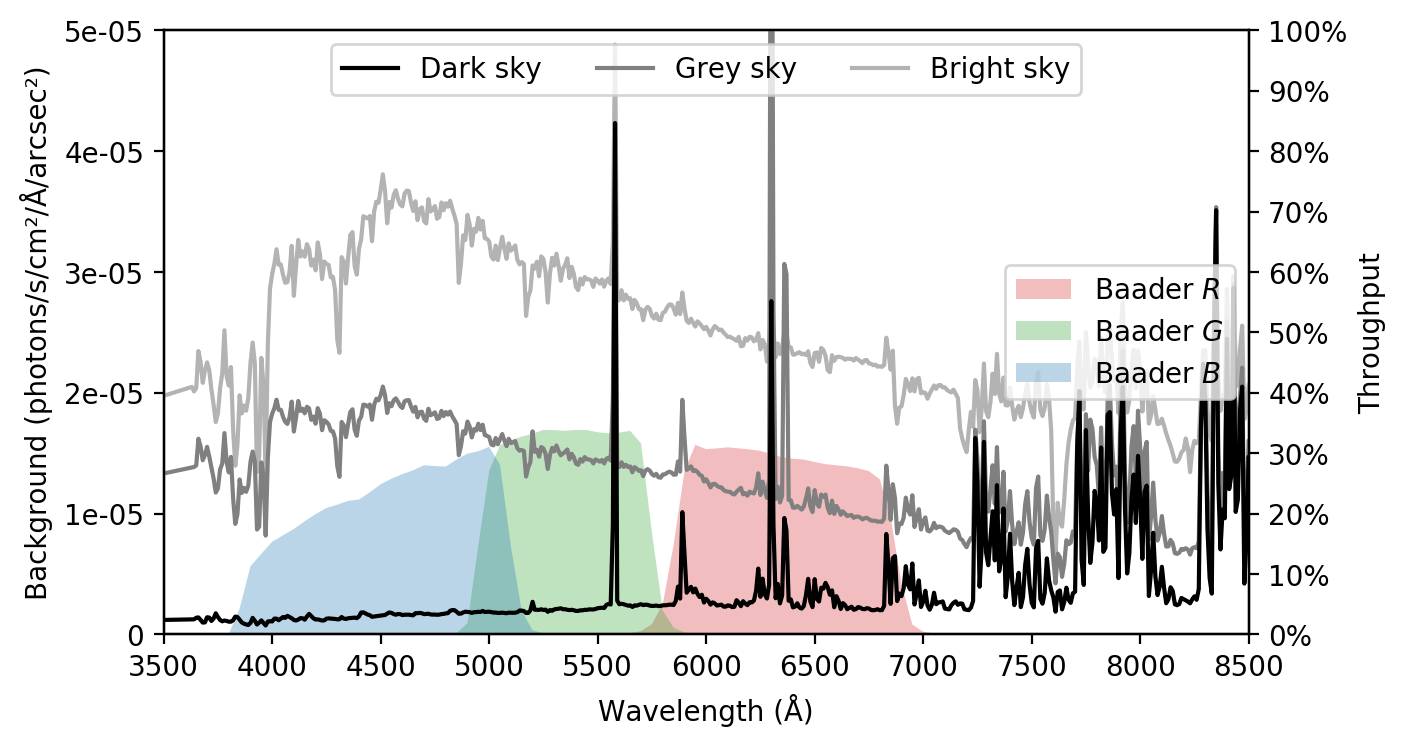
\includegraphics[width=\textwidth]{images/throughput/background.png}
    \end{center}
    \caption[Simulating sky background observations]{
        Simulating sky background observations in the GOTO filters using pysynphot. Compare to \aref{fig:pysynphot}.
    }\label{fig:background}
\end{figure}

The one value in \aref{eq:snr} that has not yet been considered is the background noise, $N_\text{BG}$. The brightness of the sky will change most noticeably as a function of the Moon phase, with a full Moon creating a background noise several magnitudes higher than during a new Moon or when the Moon is below the horizon. In order to model the background spectra were taken from \citet{sky_background}, which includes background spectra taken from 6 years of VLT observations using the FORS1 instrument\footnote{Spectra available at \href{http://www.eso.org/~fpatat/science/skybright}{\texttt{http://www.eso.org/\raisebox{0.5ex}{\texttildelow}fpatat/science/skybright}}}. Three sample spectra were selected to give a range of background signals: a ``Dark'' spectrum taken when the Moon was new and below the horizon, a ``Grey'' spectrum taken when the Moon was 60\% illuminated and a ``Bright'' spectrum when taken when the Moon was full. These spectra are shown in \aref{fig:background}.

The spectra were again convolved with the throughput model for each filter, and multiplied by the collecting area of the telescope, in order to get an expected signal in electrons per second. These were converted into instrumental magnitudes using \aref{eq:ins_mag} and then into true magnitudes using \aref{eq:zp} and the AB zeropoints given in \aref{tab:pysynphot_zeropoints}. The resulting background signals are given in \aref{tab:pysynphot_background}. Note that the background is given per square arcsecond; when calculating the background flux the signal must be multiplied by plate scale of the camera to get the signal per pixel (1.24 arcseconds/pixel for the MicroLine cameras).

\begin{table}[t]
    \begin{center}
        \begin{tabular}{c|ccc|ccc} %chktex 44
                   & \multicolumn{6}{c}{Background signal} \\
            Filter &
            \multicolumn{3}{c|}{(\elec/s/arcsec$^2$)} &
            \multicolumn{3}{c}{(mag/s/arcsec$^2$)} \\
                   & Dark & Grey & Bright & Dark & Grey & Bright \\
            \midrule
            Baader \textit{L} & 2.58 & 14.27 & 27.13 & 21.44 & 19.58 & 18.88 \\
            Baader \textit{R} & 1.18 &  4.37 &  8.20 & 20.99 & 19.58 & 18.89 \\
            Baader \textit{G} & 0.81 &  4.56 &  8.99 & 21.45 & 19.57 & 18.83 \\
            Baader \textit{B} & 0.52 &  5.74 & 10.65 & 22.20 & 19.60 & 18.93 \\
        \end{tabular}
    \end{center}
    \caption[Sky background signals calculated using pysynphot]{
        Sky background signals calculated using pysynphot for different Moon phases.
    }\label{tab:pysynphot_background}
\end{table}

% ---------
\subsubsection{Calculating limiting magnitudes}

The limiting magnitude of a telescope is defined by the signal which would be required to get over a particular SNR, for example $5\sigma$. \aref{eq:snr} therefore can be rearranged into a quadratic formula
%
\begin{equation}
    N_\text{lim}^2 - \text{SNR}^2 N_\text{lim} + \text{SNR}^2 (N_\text{BG} + D + R^2) = 0,
    \label{eq:snr2}
\end{equation}
%
and this can be solved to find $N_\text{lim}$.

It is important to remember that $N_\text{lim}$, $N_\text{BG}$ and $D$ are in electrons per second per pixel while $R$ is just in electrons per pixel (as the read-out noise is independent of the exposure time). Each therefore needs to be multiplied by the number of pixels the source is spread across, which will be the determined by the the size of the seeing disk. A given seeing $s$ in arcseconds is defined as the \glsfirst{fwhm} of the seeing disk in the image, and number of pixels the source will be spread across is
%
\begin{equation}
    n = \pi {\left(3 \frac{0.5s}{p}\right)}^2,
    \label{eq:seeing}
\end{equation}
%
where $p$ is the plate scale in arcseconds/pixel and the factor of three comes from taking the $3\sigma$ radius (note as the seeing is the FWHM it must be halved to get the radius).

Finally, the limiting magnitude in each filter and telescope can be calculated for a range of exposure times. These are plotted in \aref{fig:lim_mags} for dark and bright skies, for each GOTO filter and camera. Note it is almost impossible to distinguish between the lines for each camera, as the fractional difference between their dark and read out noise values are very small. The limiting magnitudes for a \SI{60}{\second} image, the typical exposure time for GOTO observations, are given in \aref{tab:lim_mags}.

\begin{figure}[t]
    \begin{center}
        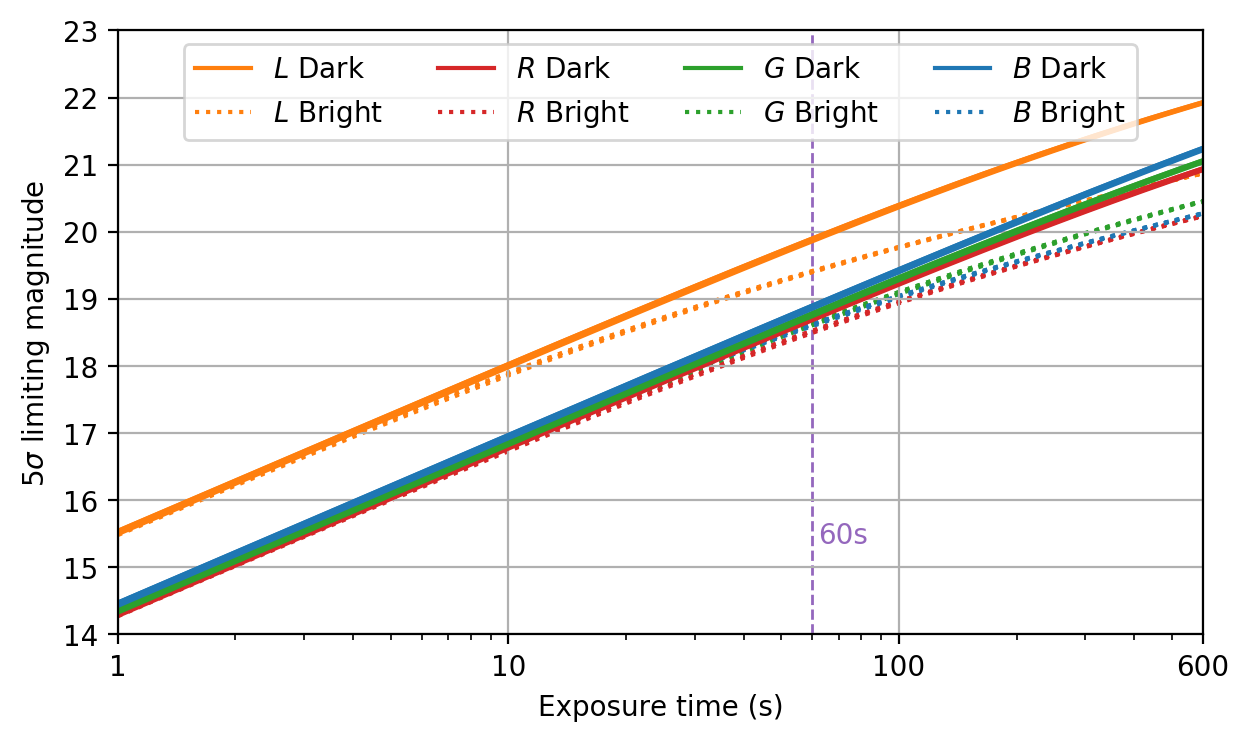
\includegraphics[width=\textwidth]{images/throughput/limiting_mag.png}
    \end{center}
    \caption[$5\sigma$ limiting magnitudes for GOTO]{
        $5\sigma$ limiting magnitudes for GOTO plotted as a function of exposure time, assuming an airmass of 1 and seeing of 1.5. Solid lines give the limiting magnitude during dark time, dotted lines during bright time. A vertical dashed line has been added at \SI{60}{\second}.
    }\label{fig:lim_mags}
\end{figure}

\begin{table}[t]
    \begin{center}
        \begin{tabular}{c|ccc} %chktex 44
                   & \multicolumn{3}{c}{Limiting magnitude} \\
            Filter & \multicolumn{3}{c}{(mag)} \\
                   & Dark & Grey & Bright \\
            \midrule
            Baader \textit{L} & 19.76 & 19.53 & 19.35 \\
            Baader \textit{R} & 18.51 & 18.43 & 18.35 \\
            Baader \textit{G} & 18.56 & 18.46 & 18.37 \\
            Baader \textit{B} & 18.85 & 18.72 & 18.62 \\
        \end{tabular}
    \end{center}
    \caption[$5\sigma$ limiting magnitudes for a \SI{60}{\second} exposure]{
        $5\sigma$ limiting magnitudes for a \SI{60}{\second} exposure.
    }\label{tab:lim_mags}
\end{table}

\end{colsection}

% ~~~~~~~~~~~~~~~~~~~~
\newpage
\subsection{Comparison to on-sky observations}
\label{sec:onsky_comparison}
\begin{colsection}

The GOTO prototype finally reached a stable 4-UT system in February 2019 (see \aref{sec:timeline}). In order to determine if it was performing to expectations the theoretical zeropoints and limiting magnitudes calculated in the previous sections can be compared to those found from real on-sky observations. Since GOTO is a very wide-field survey instrument there was no need to observe a particular standard star or field --- each frame contains thousands of individual sources that could be matched to a reference catalogue. In this case a set of sample observations were used: three \SI{60}{\second} exposures in all four filters (12 in total) of the Virgo Cluster, taken on the 16th of March 2019. These observations were taken during dark time and when the target was at a high altitude (airmass 1.08).

Each image was processed using the standard GOTOphoto pipeline (described in \aref{sec:gotophoto}), which calibrated the frames and extracted source counts using Source Extractor \citep{SE}. These counts were background-subtracted and converted into instrumental magnitudes using \aref{eq:ins_mag}, with $t=60$ and using the gain values for each camera calculated in \aref{sec:ptc}.

As GOTO uses the non-standard Baader filters (see \aref{sec:filters}) there are no exact catalogue magnitudes to compare to. The GOTO pipeline instead makes do with the best available catalogues: the Pan-STARRS PS1 catalogue \citep{Pan-STARRS} and APASS, the AAVSO Photometric All-Sky Survey \citep{APASS}. The \textit{L} and \textit{G} Baader filters are matched to Pan-STARRS \textit{g}, \textit{R} to Pan-STARRS \textit{r} and \textit{B} to APASS \textit{B}.

\begin{figure}[t]
    \begin{center}
        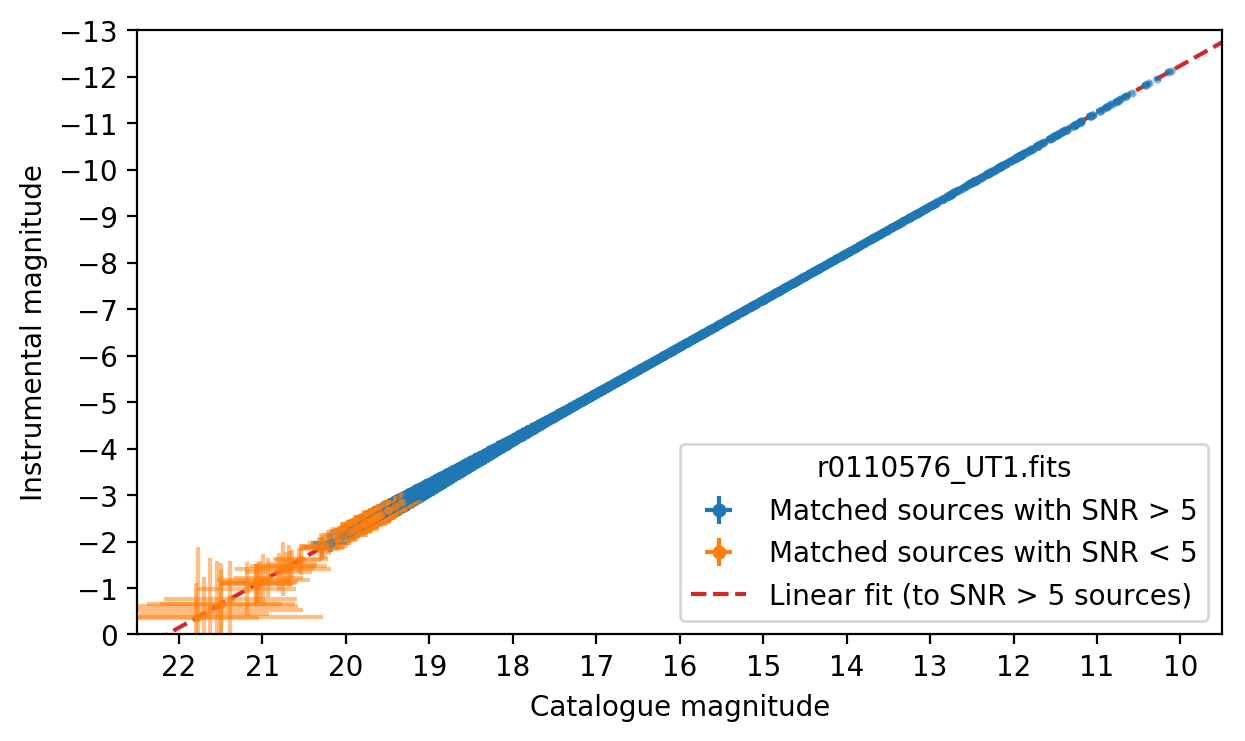
\includegraphics[width=\textwidth]{images/throughput/zeropoint_real.png}
    \end{center}
    \caption[Finding the observed zeropoint from a GOTO image]{
        Finding the observed zeropoint from a GOTO image.
    }\label{fig:zeropoint}
\end{figure}

In order to find the zeropoint for each image a linear function was fitted between the measured instrumental magnitudes of each source and the catalogue magnitude of the star it was matched against, with the y-intercept being equal to the zeropoint for that image. This is shown in \aref{fig:zeropoint} for one of the \textit{L}-band images. To exclude low-magnitude sources with large errors when fitting only sources with an SNR of 5$\sigma$ or above were included. This was repeated for every image, and the zeropoints for each are given in \aref{tab:zps_lms}.

To find the limiting magnitude the catalogue magnitude of each source was compared to the ratio of the source count and its measured noise. The $5\sigma$ limiting magnitude was taken as the mean magnitude of sources with a signal to noise ratio between 4.5 and 5.5. This method is plotted in \aref{fig:lim_mag}, and the limiting magnitude values and error values are also given in \aref{tab:zps_lms}.

\newpage

\begin{figure}[t]
    \begin{center}
        \includegraphics[width=\textwidth]{images/throughput/limiting_mag_real.png}
    \end{center}
    \caption[Finding the limiting magnitude from a GOTO image]{
        Finding the limiting magnitude from a GOTO image.
    }\label{fig:lim_mag}
\end{figure}

For each filter/unit telescope combination the best zeropoints and limiting magnitudes were selected from each set of three. These are given in \aref{tab:zps_comparison} and \aref{tab:lms_comparison}, and are compared to the theoretical AB magnitude zeropoints from \aref{tab:pysynphot_zeropoints} and the theoretical limiting magnitudes from \aref{tab:lim_mags}. In most cases the observed zeropoints and limiting magnitudes are very close to the theoretical values. Further images taken over more nights are needed to make any firm conclusions, but a few trends are clear. UT3 consistently has a better zeropoints than the others, which might be because its mirrors were serviced and returned only a month before the images were taken. Therefore the deficit in the observed zeropoints may be due to dust or imperfections that build up on the mirrors and reduce the throughput. It also seems that the throughput in the \textit{G} band has been underestimated, as the observations have higher zeropoints and better limiting magnitudes than predicted. This may be due to the bandwidth being wider than modelled, as any other change in throughput would also affect the other filters.

\newpage

\begin{table}[p]
    \begin{center}
        \begin{tabular}{cc|cc|cc|cc|cc} %chktex 44
             & &
            \multicolumn{2}{c|}{UT1} &
            \multicolumn{2}{c|}{UT2} &
            \multicolumn{2}{c|}{UT3} &
            \multicolumn{2}{c}{UT4}
            \\
             & &
            \multicolumn{2}{c|}{{\footnotesize(ML6094917)}} &
            \multicolumn{2}{c|}{{\footnotesize(ML0010316)}} &
            \multicolumn{2}{c|}{{\footnotesize(ML0420516)}} &
            \multicolumn{2}{c}{{\footnotesize(ML5644917)}}
            \\
            \multicolumn{2}{c|}{Filter} &
            ZP & LM & ZP & LM & ZP & LM & ZP & LM \\
            \midrule
            \textit{L} & 1 &
            22.32 & $19.6 \pm 0.2$ &
            22.31 & $19.7 \pm 0.3$ &
            22.40 & $19.7 \pm 0.2$ &
            22.32 & $19.6 \pm 0.1$
            \\
            & 2 &
            22.26 & $19.6 \pm 0.2$ &
            22.27 & $19.6 \pm 0.2$ &
            22.44 & $19.7 \pm 0.2$ &
            22.37 & $19.6 \pm 0.4$
            \\
            & 3 &
            22.39 & $19.6 \pm 0.2$ &
            22.42 & $19.8 \pm 0.4$ &
            22.45 & $19.7 \pm 0.2$ &
            22.40 & $19.6 \pm 0.3$
            \\
            \midrule
            \textit{R} & 1 &
            20.83 & $18.4 \pm 0.2$ &
            21.05 & $18.4 \pm 0.2$ &
            21.10 & $18.5 \pm 0.1$ &
            21.05 & $18.3 \pm 0.3$
            \\
            & 2 &
            20.84 & $18.4 \pm 0.2$ &
            21.11 & $18.5 \pm 0.3$ &
            21.13 & $18.4 \pm 0.2$ &
            21.06 & $18.3 \pm 0.3$
            \\
            & 3 &
            20.91 & $18.3 \pm 0.2$ &
            21.01 & $18.5 \pm 0.4$ &
            21.04 & $18.4 \pm 0.2$ &
            20.94 & $18.3 \pm 0.1$
            \\
            \midrule
            \textit{G} & 1 &
            21.20 & $18.7 \pm 0.2$ &
            21.39 & $18.8 \pm 0.3$ &
            21.40 & $18.8 \pm 0.2$ &
            21.27 & $18.7 \pm 0.3$
            \\
            & 2 &
            21.16 & $18.7 \pm 0.2$ &
            21.43 & $18.8 \pm 0.3$ &
            21.46 & $18.8 \pm 0.2$ &
            21.36 & $18.7 \pm 0.3$
            \\
            & 3 &
            21.26 & $18.7 \pm 0.2$ &
            21.44 & $18.8 \pm 0.2$ &
            21.45 & $18.8 \pm 0.1$ &
            21.32 & $18.6 \pm 0.2$
            \\
            \midrule
            \textit{B} & 1 &
            21.22 & $19.0 \pm 0.2$ &
            21.35 & $19.1 \pm 0.3$ &
            21.43 & $19.1 \pm 0.2$ &
            21.27 & $19.1 \pm 0.4$
            \\
            & 2 &
            21.22 & $19.0 \pm 0.2$ &
            21.32 & $19.0 \pm 0.4$ &
            21.44 & $19.1 \pm 0.2$ &
            21.22 & $19.1 \pm 0.3$
            \\
            & 3 &
            21.20 & $19.1 \pm 0.2$ &
            21.35 & $19.0 \pm 0.4$ &
            21.44 & $19.1 \pm 0.2$ &
            21.26 & $19.1 \pm 0.3$
            \\
        \end{tabular}
    \end{center}
    \caption[Observed zeropoints and limiting magnitudes]{
        Observed zeropoints and limiting magnitudes from three \SI{60}{\second} exposures taken in each filter. The camera serial numbers can be matched to \aref{tab:cameras}.
    }\label{tab:zps_lms}
\end{table}

\begin{table}[p]
    \begin{center}
        \begin{tabular}{c|c|cccc|cccc} %chktex 44
             &
            Theoretical &
            \multicolumn{4}{c|}{Best observed zeropoint} &
            \multicolumn{4}{c}{Difference (obs-theory)}
            \\
            Filter & zeropoint & UT1 & UT2 & UT3 & UT4 & UT1 & UT2 & UT3 & UT4 \\
            \midrule
            \textit{L} & 22.47 & 22.39 & 22.42 & 22.45 & 22.40 & -0.08 & -0.05 & -0.02 & -0.07 \\
            \textit{R} & 21.18 & 20.91 & 21.11 & 21.13 & 21.06 & -0.27 & -0.07 & -0.05 & -0.12 \\
            \textit{G} & 21.22 & 21.26 & 21.44 & 21.46 & 21.36 & +0.04 & +0.22 & +0.24 & +0.14 \\
            \textit{B} & 21.50 & 21.22 & 21.35 & 21.44 & 21.27 & -0.28 & -0.15 & -0.06 & -0.23 \\
        \end{tabular}
    \end{center}
    \caption[Comparison between theoretical and observed zeropoints]{
        Comparison between the best observed zeropoints and the theoretical AB magnitude zeropoints from \aref{tab:pysynphot_zeropoints}.
    }\label{tab:zps_comparison}
\end{table}

\begin{table}[p]
    \begin{center}
        \begin{tabular}{c|c|cccc} %chktex 44
             &
            Theoretical &
            \multicolumn{4}{c}{Best observed limiting magnitude}
            \\
            Filter & limiting magnitude & UT1 & UT2 & UT3 & UT4 \\
            \midrule
            \textit{L} & 19.76 & $19.6 \pm 0.2$ & $19.8 \pm 0.4$ & $19.7 \pm 0.2$ & $19.6 \pm 0.3$ \\
            \textit{R} & 18.51 & $18.4 \pm 0.2$ & $18.5 \pm 0.3$ & $18.5 \pm 0.1$ & $18.3 \pm 0.3$ \\
            \textit{G} & 18.56 & $18.7 \pm 0.2$ & $19.8 \pm 0.3$ & $18.8 \pm 0.2$ & $18.7 \pm 0.3$ \\
            \textit{B} & 18.85 & $19.1 \pm 0.2$ & $19.1 \pm 0.3$ & $19.1 \pm 0.2$ & $19.1 \pm 0.3$ \\
        \end{tabular}
    \end{center}
    \caption[Comparison between theoretical and observed limiting magnitudes]{
        Comparison between the best observed limiting magnitudes and the theoretical dark-time limiting magnitudes from \aref{tab:lim_mags}.
    }\label{tab:lms_comparison}
\end{table}

\clearpage

\end{colsection}

% ~~~~~~~~~~~~~~~~~~~~

\end{colsection}

% ########################################

\chapter{The GOTO Telescope Control System}
\label{chap:gtecs}
\chaptoc{}

% ########################################

\newpage
\section{Introduction}
\label{sec:gtecs_intro}
\begin{colsection}

% ~~~~~~~~~~~~~~~~~~~~

\begin{colsection}

In this chapter I outline my work creating a control system for the GOTO prototype telescope. Sections~\ref{sec:gtecs},~\ref{sec:hardware_control} and~\ref{sec:autonomous} are expanded from my SPIE conference paper~\citet{Dyer}. The GOTO Telescope Control System is based on the pt5m control system~\citep{pt5m}, written primarily by Tim Butterly, Stu Littlefair and Vik Dhillon. This provided the foundation that the GOTO system builds upon, but has been heavily modified and rewritten to meet the requirements of the GOTO project. All work described is my own, incorporating advice and feedback from members of the GOTO collaboration.

\end{colsection}

% ~~~~~~~~~~~~~~~~~~~~

\subsection{Requirements of the control system}
\label{sec:control_requirements}
\begin{colsection}

My first task as part of the GOTO collaboration, in the summer before I started in Sheffield, was to decide on what control system software to use for the telescope. There were several requirements to consider.

Firstly the chosen system had to allow for remote and, most importantly, robotic operation of GOTO.\@ There are many telescope software packages available, but the majority are designed for a human observer to operate. GOTO however was to be a fully autonomous telescope, which meant operating nightly with no human intervention. This meant the control system had to contain routines for observing targets and standard tasks like taking calibration frames. On top of that it was desirable for the system to be able to monitor itself to detect and fix any errors as much as possible without the need for human intervention. Finally it had to be able to monitor and react to external conditions, for example closing the dome if rain was detected.

Secondly the system had to include an observation scheduler, which could decide what the telescope should observe during the night. A basic scheduler might be run in the evening to create a night plan, as observers typically do when operating a telescope. However that alone would not fit the expected operations required from GOTO:\@ normally carrying out an all-sky survey but with a robust interrupt protocol for gravitational wave follow-up. The system therefore had to be able to recalculate what to observe on-the-fly, and be able to immediately react to transient \gls{too} events.

Furthermore, although the project was still at an early stage the idea of linking together multiple telescopes into a global network was also considered, and the chosen control system implementation would ideally be expandable to facilitate this in the future (or at least not hinder the possibility).

There were also several physical considerations when it came to choosing between software systems. The telescope hardware had already been decided on: an Astrohaven clamshell dome\footnote{Astro Haven Enterprises, CA, USA;\@ (\url{www.astrohaven.com})}, a custom mount with a \gls{sitech} servo controller\footnote{Sidereal Technology, OR, USA;\@ (\url{www.siderealtechnology.com})} and multiple unit telescopes all using \gls{fli} cameras, focusers and filter wheels\footnote{Fingerlake Instruments, NY, USA;\@ (\url{www.flicamera.com})}. Any control system would need to communicate with all of them, so any systems with existing drivers or packages used by established projects would be desirable. \rtxt{Move links to hardware section}

Two particular hardware-related challenges faced the control system project. The first was that the SiTech controller software, \software{SiTechEXE}, only ran on Microsoft Windows. The software did have an accessible \gls{api} through the \software{ASCOM} standard\footnote{\url{www.ascom-standards.org}} but that still required some form of the mount control system to be running on Windows. As most scientific software in astronomy runs on Linux systems this lead to two options: either have just a small interface running on the Windows machine and the majority of the system on Linux, or have the entire system run on Windows.

The second challenge was to deal with the multiple-unit telescope design of \gls{goto}. A full array of eight \glspl{ut} would require eight cameras, focusers and filter wheels. These would all need to be run in parallel, most importantly there needed to be no delay between the exposures starting and finishing on each camera. The physical construction of the telescope also came into play. The \gls{fli} units all require a USB connection to the control computer. A single computer situated in the dome would therefore require 24 USB cables to run up the mount, not only a practical difficulty but also a layout that could lead to interference and data loss. The suggested solution was to have small computers attached to the mount boom arms to act as intermediate interfaces to the \gls{ut} hardware. The control system therefore needed to be able to run in a distributed manner across multiple computers, potentially even running different operating systems.

Finally, there were practical details to consider. \gls{goto} was designed as a relatively inexpensive project that could be built quickly and copied across multiple sites, therefore any costly software licenses would ideally be avoided. Experience and support requirements should also be considered, and reusing a system that members of the collaboration had experience with would provide benefits compared to a completely new and exotic system.

\end{colsection}

% ~~~~~~~~~~~~~~~~~~~~

\subsection{Different control system options}
\label{sec:control_options}
\begin{colsection}

Four possible options for the GOTO control systems were considered: the existing software packages \software{ACP Expert}, \software{Talon} and \software{RTS2} or a custom system based on the code written for the \gls{pt5m}. At the July 2015 GOTO meeting at Warwick University I gave a talk outlining the control system requirements and presenting the four options, and the decision taken was to adapt the \gls{pt5m} system for use by GOTO.\@ The three rejected systems are described below, while the \gls{pt5m} system is described in more detail in Section~\ref{sec:pt5m}.

\subsubsection{\software{ACP Expert}}
\software{ACP Expert}\footnote{\url{http://acp.dc3.com}} is a commercial observatory control software system by DC3-Dreams. It is used by some advanced amateur astronomers and a few scientific and university telescopes, such as the Open University's \gls{pirate} \citep{PIRATE}. As a complete Windows software package with a web interface it is marketed as being straightforward to use, in either remote or fully robotic modes. It uses the \software{ASCOM} standard library and DC3-Dreams also provide professional support and updates. This however came at a cost: \$2495 for the base software, plus an additional \$599 for Maxim DL camera control and \$650 per year for continued support. At the time \gls{goto} was anticipated to be deployed in a matter of months, so the quick and simple pre-existing commercial solution was tempting. However it was unsure if the \software{ACP} software would be able to cope with \gls{goto}'s unusual design, and its closed-source model would restrict our ability to make modifications.

\subsubsection{\software{Talon}}

The \software{Talon} observatory control system\footnote{\url{https://observatory.sourceforge.io}} is a Linux-based, open-source system created by \gls{omi}. It was included as an option primarily as at the time it was the control system of choice for the other observatories operated by Warwick University, such as SuperWASP \citep{SuperWASP}. \gls{omi} had built the SuperWASP mount and developed \software{Talon} alongside it, before later making it open source. However as a programme development has been limited to non-existent over the past decade, and Warwick were already looking at replacing it for their \gls{w1m} telescope and, ultimately, when upgrading SuperWASP.\@ Therefore adopting it for \gls{goto} would be unlikely and even counter-productive, as whatever was chosen for \gls{goto} was expected to (and ultimately did) influence and benefit the concurrent development of a new control system for \gls{w1m}.

\subsubsection{\software{RTS2}}

The \gls{rts2}\footnote{\url{https://rts2.org}} \citep{RTS2, RTS2b} is another free and open-source Linux software package. Unlike \software{Talon}, \software{RTS2} is under active development and is used by telescopes and observatories around the world \citep{BORAT, BOOTES-3, antarctic, ARTN}. There is a small but active community and multiple different drivers for the hardware \gls{goto} would use have been developed. The first version of RTS was written in \proglang{Python}, while the second version was rewritten in \proglang{C++} but with a \proglang{Python} interface available. \gls{rts2} was an attractive choice, however like the others it was unclear if it could be easily modified to meet the requirements for \gls{goto}'s multiple telescopes and Windows-controlled mount and no one in the collaboration had prior experience of using or implementing it.

\end{colsection}

% ~~~~~~~~~~~~~~~~~~~~

\subsection{The \textit{pt5m} control system}
\label{sec:pt5m}
\begin{colsection}

Built and operated by Sheffield and Durham Universities, \gls{pt5m} is a small \SI{0.5}{\metre} telescope located on La Palma on the roof of the \gls{wht} \citep{pt5m}. The telescope was originally developed as a \gls{slodar} system for atmospheric turbulence profiling \citep{SLODAR_LaPalma} and is one of several around the world operated by Durham, including one in Korea that had just been commissioned at the time I joined GOTO \citep{SLODAR_Korea}. In order to make the most of the telescope when not being used for \gls{slodar} observations a science camera was added to \gls{pt5m} and it was upgraded for robotic observations. Since it has successfully been used for automatic observations of transient events, as well as being used for undergraduate teaching at Sheffield and Durham. All the \gls{slodar} telescopes used a custom control system developed at Durham, and a similar system was used by the teaching telescopes of the Durham Department of Physics that I worked with during my undergraduate program. The \gls{pt5m} system has been modified for its extra roles which matched well to what we needed for \gls{goto}, and so it was chosen to be the base for the GOTO control system.

The \gls{pt5m} control system is written in \proglang{Python} and was built around multiple independent hardware daemon programs with a pilot program to control them. This basic framework was adopted for \gls{goto}, with some changes. The major obvious difference between \gls{pt5m} and \gls{goto} are the multiple unit telescopes, but the same system could be adapted through the creation of interface daemons on which allow communication to the unit telescopes over the network. In fact the nature of the daemon system made it very easy to expand to have daemons running on physically separate machines but still communicate over the network, including on both Linux and Windows computers. This also made it possible to run the scheduler and sentinel on the database machine, a key detail for the multiple-telescope system.

\begin{figure}[p]
\begin{center}
\includegraphics[width=\linewidth]{images/pt5m_software.png}
\end{center}
\caption[The pt5m control system architecture]{The \gls{pt5m} control system architecture, taken from~\cite{pt5m}. The hardware daemons are shown on the right, they communicate with the pilot which receives information from the observation scheduler and the conditions monitor. This basic framework was adapted for the GOTO control system, c.f. Figure~\ref{fig:flow}.}
\label{fig:pt5m_software}
\end{figure}

\end{colsection}

% ~~~~~~~~~~~~~~~~~~~~

\end{colsection}

% ########################################

\newpage
\section{Overview of G-TeCS}
\label{sec:gtecs}
\begin{colsection}

% ~~~~~~~~~~~~~~~~~~~~

\begin{colsection}

The \gls{gtecs} is the name given to the collection of programs and systems that have been developed to fulfil the requirements of the GOTO project. The \gls{pt5m} control system as described in the previous section formed the basis for \gls{gtecs}. Its structure of multiple independent daemons was developed into the core system architecture, shown in Figure~\ref{fig:flow}. This section gives an overview of the system and its implementation, and the following sections discuss in detail the two core branches of G-TeCS:\@ the base hardware control programmes (Section~\ref{sec:hardware_control}) and autonomous systems built on top of them (Section~\ref{sec:autonomous}).


\begin{figure}[p]
\begin{center}
\includegraphics[width=\linewidth]{images/flow.pdf}
\end{center}
\caption[The G-TeCS system architecture]{The \gls{gtecs} system architecture as deployed on La Palma. The observation database as well as the sentinel, scheduler and conditions daemons shown to the left run on an observatory-wide master server, while the pilot and hardware daemons are located on the telescope control computer within the dome. Control for the unit telescope hardware (focuser, filter wheel and camera) is sent via an interface daemon for each pair of UTs, running on computers attached to the mount. Only the system for the prototype instrument (one mount with four unit telescopes) is shown.}
\label{fig:flow}
\end{figure}

\end{colsection}

% ~~~~~~~~~~~~~~~~~~~~

\subsection{Implementation}
\label{sec:implementation}
\begin{colsection}

The core \gls{gtecs} code is written as a \proglang{Python} package, \pkg{gtecs}. This includes all the daemons, scripts, associated modules and functions. One core component, the code and functions to interact with the observation database (see Section~\ref{sec:obsdb}), has been split off into a separate \proglang{Python} package ObsDB (\pkg{obsdb}), this was to allow other users to interact with the database without the need to install the entire \pkg{gtecs} package. In addition, the code for alert processing within the sentinel (see Section~\ref{sec:sentinel}) is in a separate module, GOTO-alert (\pkg{gotoalert}). This is because it originated as a separate code project developed by Alex Obradovic at Monash, that I then took over and integrated with the \gls{gtecs} sentinel. GOTO-alert is described in more detail in Section~\ref{sec:gotoalert}.

G-TeCS and the associated packages are written almost entirely in \proglang{Python}, specifically \proglang{Python3}. \proglang{Python} is a versatile programming language that is increasingly common in astronomy, helped by the popular open-source Astropy Project \citep{astropy}. \proglang{Python} version 3.0 was released in 2008 and is infamously not backwards-compatible with \proglang{Python2}. The code for \gls{pt5m} was written in \proglang{Python2}, and therefore initially so was G-TeCS.\@ Over the subsequent years the code was re-written to be compatible with both \proglang{Python2} and \proglang{Python3}, which was possible due to the inbuilt \code{\_\_future\_\_} module in \proglang{Python2} and the \code{six} package. Finally the addition of new features added to \proglang{Python3}, such as the \pkg{asyncio} package (used heavily by the pilot) in version 3.5, and the imminent end-of-life of \proglang{Python2} in 2020 lead to the dropping of \proglang{Python2} support. This is in line with most other scientific \proglang{Python} packages including \pkg{astropy}, which is no longer developed for \proglang{Python2}. % chktex 21

The \pkg{gtecs} and associated packages have a variety of requirements. Some of the most critical external packages (not included in the \proglang{Python} standard library) are \pkg{numpy} for mathematical and scientific structures, \pkg{astropy} for astronomical functions, \pkg{sqlalchemy} for \proglang{SQL} database management (see Section~\ref{sec:obsdb}), \pkg{astroplan} for scheduling (see Section~\ref{sec:scheduler}), \pkg{voeventparse} for handling VOEvents (Section~\ref{sec:sentinel}) and \pkg{gototile} for sky map processing (Section~\ref{sec:gototile}).

\end{colsection}

% ~~~~~~~~~~~~~~~~~~~~

\subsection{Daemons}
\label{sec:daemons}
\begin{colsection}

The core elements of the control system are the daemons. A \emph{daemon} is a type of computer program that runs as a background process, continually cycling and awaiting any input from the user. This is in contrast to a \emph{script} which is run once (either by the system or a user), carries out a series of tasks in the foreground and then exits once it is completed. Common examples of daemons on a Unix-based system are \software{sshd}, which listens for and creates \gls{ssh} connections, and \software{cron}, which runs commands at predefined times. Incidentally both are used by G-TeCS:\@ \gls{ssh} to issue commands on remote machines and \software{cron} to start scripts like the pilot at a set time.

Daemons are the ideal form of software for hardware control. Once started each daemon runs continually as a background process, with a main control loop that repeats on a regular timescale (for the G-TeCS hardware daemons this is usually every \SI{0.1}{\second}). There are two primary tasks that are carried out within the loop by every daemon: monitoring the status of the hardware, and listening for and carrying out input commands. The former is typically not carried out every time the loop runs, because attempting to request and process the hardware status every \SI{0.1}{\second} would overwhelm the daemon and delay the loop. Instead the status checks are typically carried out every \SI{2}{\second}, or sooner if requested. By continually requesting the status of the hardware the daemon will detect very quickly if there are any problems, and should they be unable to reach their hardware they will enter an error state. However the daemons themselves will not attempt to self-diagnose and fix any problems that are detected, with the notable exception of the dome daemon (Section~\ref{sec:dome}). Instead that is the job of the hardware monitors (see Section~\ref{sec:pilot}), the daemons themselves will just report any problems to the pilot or user. The second reason for a control loop within the daemons is to listen for and carry out any commands issued to them. As these commands are dealt with within the loop it insures only one is carried out at once, the alternative of user input going directly to the hardware could cause problems with overlapping commands. These commands can be as simple as querying the cameras for how long left until an exposure finishes to opening the dome, taking and saving an image or calculating the current highest priority pointing to observe.

Within G-TeCS each category of hardware has a dedicated control daemon that acts as an interface to the hardware. For example, the mount daemon communicates with the SiTech mount controller, sending commands and reading the current status, while the camera daemon does the same for every camera attached to the telescope. Therefore there is not necessarily a one-to-one correspondence between daemons and pieces of hardware. Although typically grouped together as ``hardware daemons'' not every daemon within G-TeCS falls into that category: there is the scheduler daemon which is the interface to the observation database and the sentinel daemon which monitors alert channels. Although not connected to physical hardware like a dome or a camera, both operate in a similar way to the others.

Functionally each daemon is built around a \proglang{Python} class which contains hardware control functions and the main loop. When the daemon starts the loop is set running in its own thread, and when a control function is called it sets a flag within this loop to carry out the requested commands. The daemons are created using the \gls{pyro} module \pkg{Pyro4}\footnote{\url{https://pythonhosted.org/Pyro4/}}. Each daemon is run as a \gls{pyro} server, so any client script can then access its functions and methods across the network using the associated server ID.\@ This system allows complicated interactions across the network between daemons and scripts with very simple code, and was one of the major benefits of using the \gls{pt5m} system.

\end{colsection}

% ~~~~~~~~~~~~~~~~~~~~

\subsection{Scripts}
\label{sec:scripts}
\begin{colsection}

As well as the daemons, the \pkg{gtecs} package includes multiple \proglang{Python} scripts. Once installed these scripts can all be run from the command line by a human, or with utilities like \software{cron}.

In order to send commands to the daemons each has an associated control script that can be called by a user from a terminal, or by the pilot in robotic mode (see Sec~\ref{sec:pilot}). The commands follow a simple format which was inherited from \gls{pt5m}, first the short name of the daemon, then the command and finally any arguments. There are several commands that are common to all daemons: \code{start}, \code{shutdown} and \code{restart} to control if the daemon is running; \code{ping} to see the current status of the daemon; \code{info} to see the current status of the hardware; \code{log} to print the daemon output log. Examples of daemon-specific commands include ``\code{dome~close}'' to close the dome, ``\code{mnt~slew~30.54~+62}'' to slew the mount to the given coordinates, ``\texttt{cam~image~60}'' to take a \SI{60}{\second} exposure with all connected cameras and ``\texttt{cam~image~2~60}'' to take a \SI{60}{\second} exposure with camera 2 only.

Every daemon can also be controlled in ``interactive mode'', which is a user-friendly way to save time sending multiple commands to the same daemon. Interactive mode is entered with \code{i} and exited with \code{q}.

There is also a utility script, \code{lilith}, which can send the same command to all the installed daemons. For example, to shutdown every daemon it is possible to call each directly (\code{cam shutdown}, \code{foc shutdown}, \code{mnt shutdown} etc\ldots) but it is instead much easier to run \code{lilith shutdown}. The name ``Lilith'' comes from the biblical ``mother of demons''.

The most important script to the robotic operation of the telescope is the pilot, an asynchronous script that is run every night using \software{cron} at 5pm. The functions carried out by the pilot and the following scripts are detailed in Section~\ref{sec:pilot}. The pilot can also be started manually with the command \code{pilot start}, which is the command defined in the \code{crontab} file used by \software{cron} (note although this uses the same syntax as a daemon it is mechanically different, as it simply runs the script in the current terminal instead of starting a background process). There is also a daytime counterpart to the pilot, called the day marshal, which is run in the same way. Finally within the pilot, several of the standard tasks are separated off into ``observation scripts'', lists of commands to the daemons to carry out tasks like focusing the telescope, taking flat fields or starting/shutting down the hardware in the evening/morning respectively. As standard tasks these can also be run by human observers though a command line script \code{obs\_script} (for example \code{obs\_script~startup} or \code{obs\_script~autofocus}).

\end{colsection}

% ~~~~~~~~~~~~~~~~~~~~

\subsection{System mode}
\label{sec:mode}
\begin{colsection}

\gls{goto} is a robotic telescope, and \gls{gtecs} is designed around that concept. This means the system will operate nightly with no human intervention needed. However sometimes it is necessary for a human operator to take control of the telescope, if one of the automated scripts fails or a situation arises that is easer to deal with manually. One example was taking observations of the asteroid Phaethon \citep{Phaethon}. The \gls{gtecs} observing database and pilot was not designed to observe solar system objects, so it was easier for a human observer to look up and slew to the coordinates. Finally there are cases when it is important that the automated systems are disabled: if work is being done to the hardware on-site it could be dangerous if the system still tried and move the mount or dome.

\gls{gtecs} deals with these situations by having an overall system mode flag stored in a datafile which can be checked by the automated systems before activating. There are three possible modes, outlined below and summarised in Table~\ref{tab:modes}.

\begin{itemize}
    \item \code{robotic} mode is the default mode for the telescope. In this case it is assumed that the system is completely automated and therefore could move at any time. In this mode during the night the pilot will be in complete control of the telescope, and the dome will automatically close in bad weather.
    \item \code{manual} mode is designed for manual observing, either on-site or remotely. In this mode the pilot will be paused and so will not interrupt commands sent by the observer. The dome will still sound the alarm when moving and autoclose in bad weather by default, but both of these features can be disabled. It is intended that they should only be disabled if there is an observer physically present in the dome, otherwise the dome should still be able to close automatically when observing remotely.
    \item \code{engineering} mode is designed to be used only if there are workers on site in situations where the system moving without warning could be dangerous. All of the dome options are automatically disabled, and the pilot and day marshal will refuse to start. Leaving the system in this state for long periods of time is undesirable, and so it should only be used when physical work is ongoing or the telescope is completely deactivated.
\end{itemize}

\begin{table}[ht]
\begin{center}
\begin{tabular}{c|ccccc} % chktex 44
mode &
pilot &
day marshal &
dome autoclose &
dome alarm &
\code{hatch} flag
\\
\midrule

\code{robotic} &
\textcolor{Green}{active} &
\textcolor{Green}{active} &
\textcolor{Green}{enabled} &
\textcolor{Green}{enabled} &
\textcolor{Green}{active}

\\

\code{manual} &
\textcolor{orange}{paused} &
\textcolor{Green}{active} &
\makecell{\textcolor{Green}{enabled} or \\ \textcolor{red}{disabled}} &
\makecell{\textcolor{Green}{enabled} or \\ \textcolor{red}{disabled}} &
\textcolor{red}{ignored}

\\

\code{engineering} &
\textcolor{red}{disabled} &
\textcolor{red}{disabled} &
\textcolor{red}{disabled} &
\textcolor{red}{disabled} &
\textcolor{red}{ignored}
\\

\end{tabular}
\end{center}
\caption[System mode comparison]{A comparison of the three \gls{gtecs} system modes. In \code{robotic} mode all the automated systems are enabled, while in \code{engineering} mode they are disabled. In \code{manual} mode the pilot is paused and the observer can disable the dome systems if desired. For more information see Section~\ref{sec:pilot} for the pilot and day marshal, Section~\ref{sec:dome} for the dome and Section~\ref{sec:conditions} for the conditions flags.}
\label{tab:modes}
\end{table}

\end{colsection}

% ~~~~~~~~~~~~~~~~~~~~

\end{colsection}

% ########################################

\newpage
\section{Hardware Control}
\label{sec:hardware_control}
\begin{colsection}

% ~~~~~~~~~~~~~~~~~~~~

\begin{colsection}

The core programmes of \gls{gtecs} are the hardware daemons. There are seven primary daemons, as shown in the centre-right of Figure~\ref{fig:flow}. This section provides a summary of each of the hardware categories, describing the how the daemons interact with them and the particular challenges and features unique to each.

\end{colsection}

% ~~~~~~~~~~~~~~~~~~~~

\subsection{FLI interfaces}
\label{sec:fli}
% transfer images as num py arrays, so pickle
% "meta-daemons"??
\begin{colsection}

\rtxt{As described in the hardware chapter}, \gls{goto} uses off-the-shelf camera hardware from \gls{fli}. Each \gls{goto} unit telescope has a MicroLine ML50100 camera, an Atlas focuser and a CFW9--5 filter wheel connected to a small Intel \gls{nuc} attached to the boom arm. On these \glspl{nuc} run very basic daemons called the \gls{fli} interfaces. Barely daemons by the definition given in Section~\ref{sec:daemons}, these interfaces have no control loop and exist only as a way to expose the serial connection of the hardware to the wider \gls{pyro} network. By using these interface daemons, the primary control daemons for the \gls{fli} hardware can run on the main control computer without being physically connected to the hardware (aside from via ethernet).

Communicating with the hardware has to be done using the \gls{sdk} provided by \gls{fli}, which is written in \proglang{C}. In order to use this \gls{sdk} with the control system written in \software{Python} a separate wrapper package \pkg{fli-api} was written in \software{Cython}, a programming language that provides a way for \proglang{C} code to be imported and run in \proglang{Python}.

The other benefit of the interfaces and the \gls{pyro} network is to allow a single daemon to interact with multiple pieces of hardware across multiple computers. This means that the single camera daemon running on the primary control computer can interface with all the cameras attached to the mount, and instead of sending commands to each camera individually the user can speak to them all together through the daemon. As an example, the command \code{cam~image~60} will take a 60 second exposure on every attached camera simultaneously. Including a specific number \code{cam~image~2~60} will only start the exposure on the camera attached to \gls{ut} 2. Multiple selections can also be made using a simple comma-separated syntax, such as \texttt{cam~image~1,2,4~60}. This notation and functionality is one of the major differences between \gls{gtecs} and the \gls{pt5m} control system, and in fact all the other control systems considered in Section~\ref{sec:control_options}, which typically only communicate with a single telescope.

There are three control daemons that interact with the \gls{fli} interfaces: the camera, filter wheel and focuser daemons. There is also a fourth, the exposure queue daemon, which coordinates sets of exposures and communicates with both the cameras and filter wheels through their daemons, not the interfaces directly. Each of the four are described in the following sections.

\end{colsection}

% ~~~~~~~~~~~~~~~~~~~~

\subsection{Camera control}
\label{sec:cam}
% how images are written
%   multiple FITS extensions considered
%   don't have space to store a whole image on the chip... (inside fli api)
% headers
%   all cards in appendix?
\begin{colsection}

The camera daemon interacts with all of the \gls{fli} cameras on a single \gls{goto} mount. This makes it the most complicated daemon, and perhaps the second-most-important after the dome daemon. The commands to the camera daemon are fairly straightforward. There are four types of exposures that can be taken with the daemon:

\begin{itemize}
    \item Normal images, with the shutter opening and closing for the given exposure time.
    \item ``Glance'' images, which are the same as standard exposures but are saved into a separate directory from the normal ``science'' images.
    \item Dark images, where the shutter remains closed during the exposure time.
    \item Bias images, which are dark images but with a zero-second exposure time.
\end{itemize}

The \pkg{fli-api} interface also gives other options for exposures aside from just the exposure time, including different binning factors and the active area of the chip to read out. Although the camera daemon does offer commands to set these they are never regularly used during normal operators, and the image processing pipeline is set up to only expect full-frame, unbinned images.

Once an exposure is completed the image data needs to be downloaded from the cameras and then sent through the interfaces to the camera daemon before the frames can be saved as \gls{fits} files. This is a disadvantage of the interface system, and consideration was given to instead having the interfaces write out the files. Although this would have been faster to save the raw images, they would still need to be copied down from the interfaces to the primary archive on the control computer. Having the interfaces send the raw count arrays to the camera daemon for processing proved to save more time in the long run. The camera daemon also has to query the other daemons at the start of the exposure to get their current statuses to add to the \gls{fits} header.

The time taken by each exposure, from the command being received to the images being created, has been optimised to minimise the amount of ``dead time'' wasted. One of the primary ways to save time was to have the two most time-dependent processes, downloading the images from the interfaces and writing them to disk, run as separate threads for each camera independently of the main daemon control loop. Other time-saving improvements included only fetching the status information from the other daemons once, just after starting the exposures (so it doesn't take any extra time in addition to the exposure time).

Images are written to \gls{fits} files by the camera daemon and are archived by date. Each camera output is saved as a separate file, named by the current run number and the name of the unit telescope it originated from (e.g. \texttt{r000033\_UT2.fits} is the image from camera 2 for run 33). The run number is increased whenever a non-glance exposure is taken. After being saved the images are copied on regular intervals from La Palma to Warwick University via a dedicated fibre link, where the photometry pipeline is run. The image processing pipeline is a separate project from the control system being worked on at Warwick and Monash, which means image calibration, astrometry and photometry are all out of the scope of this thesis.

\end{colsection}

% ~~~~~~~~~~~~~~~~~~~~

\subsection{Filter wheel control}
\label{sec:filt}
% filter profiles? no, see throughput section
\begin{colsection}

The filter wheel daemon (sometimes shortened to just the filter daemon) controls the filter wheels on the \gls{goto} unit telescopes. The \gls{fli} CFW9--5 filter wheels are fairly standard pieces of hardware, with 5 slots that contain the Baader R, G, B, L and C filters (\rtxt{see throughput section}). Moving the filter wheel is typically done via the exposure queue daemon (see Section~\ref{sec:exq}) but can be done individually. When being restarted the filter wheels need to be homed to position 0, which contains the L filter. This was intentional as a vast majority of typical \gls{goto} observations are taken in the luminance filter instead of colours.

The only major complication in creating the filter wheel control code was identifying the hardware pieces when connected to the interface \glspl{nuc}. The initial set of CFW9--5 units were not serialised, i.e.\ they did not have serial numbers defined. The usual way to connect to specific hardware units through \pkg{fli-api} is to search the connected USB devices for their unique serial numbers. This was a problem for the filter wheels, and as two wheels were connected to each \gls{nuc} it was impossible to tell them apart. A workaround was developed using the \proglang{Python} \pkg{pyudev} module, that uses the Linux \code{udev} device manager to identify devices using their unique device names. This feature as patched into \pkg{fli-api} and enabled the control system to individually tell apart the connected filter wheels.

\end{colsection}

% ~~~~~~~~~~~~~~~~~~~~

\subsection{Focuser control}
\label{sec:foc}
\begin{colsection}

The focuser daemon is the third of the three \gls{fli} hardware daemons, and is also fairly simple. Each connected filter can be set to a specific position or moved by a given offset, this is used almost exclusively when the pilot runs the autofocus routine at the start of the night (see Section~\ref{sec:pilot}) \rtxt{autofocus section?}.

\end{colsection}

% ~~~~~~~~~~~~~~~~~~~~

\subsection{Exposure queue control}
\label{sec:exq}
\begin{colsection}

The exposure queue daemon (often abbreviated to ExQ or `exq') is unusual amongst the daemons, as it does not directly talk to hardware. Instead it is the only daemon that's primary purpose is communicating with other daemons, specifically the camera and filter wheel daemons. The exposure queue daemon coordinates taking frames in sequence and setting filters before the exposures start. Consider wanting a series of \SI{30}{\second} exposures in the R, G and B filters. Through the camera and filter wheel daemons this would require six commands: \code{filt~set~R}, \code{cam~image~30}, \code{filt~set~G}, \code{cam~image~30} etc. The exposure que daemon however gives a way to shortcut this, and the same exposures can be requested with a single command (\code{exq mimage 30 R,G,B} in this case).

\begin{figure}[t]
\begin{center}
\vspace{1cm}
\code{1111;30;R;1;normal;M101;SCIENCE;0;1;3;545}\\
\code{1111;30;G;1;normal;M101;SCIENCE;0;2;3;545}\\
\code{1111;30;B;1;normal;M101;SCIENCE;0;3;3;545}\\
\vspace{0cm}
\end{center}
\caption[A sample exposure queue file]{A sample of an exposure queue file. Each line is a new exposure, and details of the exposure are separated by semicolons. In order these are the \gls{ut} mask, exposure time, filter, binning factor, frame type, object name, image type, glance flag, set position, set total and database ID number.}
\label{fig:exq_file}
\end{figure}

When a set of exposures is defined and passed to the exposure queue daemon the are added to the queue, which is a physical file written to and read by the daemon. An example of the contents of the file is given in Figure~\ref{fig:exq_file}. The details of each exposure are saved in this file, and adding more using the \code{exq} commands adds more exposures to the end of the queue. When the queue is running (it can be paused and resumed, to allow for example slews between exposures) the daemon will select the first exposure in the queue, tell the filter wheel daemon to change filter if necessary and then tell the cam daemon to start the exposure.

As shown in Figure~\ref{fig:exq_file} extra meta-data can be written for each exposure. The \gls{ut} mask is simply a binary representation of the unit telescopes to use for this exposure, so \code{0101} would be exposing on \glspl{ut} 1 and 3 only (counting from the right), while \code{1111} will be on all four. The frame type is a variable used within \pkg{fli-api}, it is either \code{normal} or \code{dark} depending on if the shutter will open or not. Exposures taken through the exposure queue can also have a target name (use to identify target objects, in the case shown in Figure~\ref{fig:exq_file} galaxy M101) and an image type (used to define the type of image, either SCIENCE, FOCUS, FLAT, DARK or BIAS). The set position and total are results of adding sets of exposures with one command, as in the example above. This is important to the image pipeline for knowing sets of, for example, 3 \SI{60}{\second} L images which are typically co-added to produce reference frames. Finally the concept of ``exposure sets'' is defined in the observing database, with each pointing having at least one or more sets defined to be added to the exposure queue by the pilot when that set is observed (see Section~\ref{sec:obsdb}).

Similar to the camera daemon, the timing of code and functions within the exposure queue daemon has been optimised to minimise any wasted ``dead time''. However the commands sent also need to be timed correctly to ensure that, for example, the exposure doesn't start while the filter wheel is still moving. This was one of the major reasons for having a separate exposure queue daemon to handle these timing concerns while the camera and filter wheel daemons dealt only with individual commands (incidentally \gls{pt5m} uses a QSI camera with an integrated filter wheel, so the \gls{gtecs} camera, filter wheel and exposure queue daemons are combined into a single ``CCD'' daemon in Figure~\ref{fig:pt5m_software}).

\end{colsection}

% ~~~~~~~~~~~~~~~~~~~~

\subsection{Dome control}
\label{sec:dome}
% limit switches + extras with Aurduino (in commissioning chapter?)
%   sometimes didn't fully open
%   closing slightly and reopening worked most of the time
%   limit switches needed adjustment
\begin{colsection}

The dome daemon is the primary interface to the Astrohaven clamshell dome. As such is in effect the most critical of all the hardware control systems, because a failure in the software meaning the dome opens in bad weather could be catastrophic to the hardware inside. As such it is one of the more complicated single hardware daemons, and includes multiple levels of checks and backup systems. It is also the only daemon with a small amount of autonomy built-in, and therefore blurs the line between a pure hardware control system and the more complicated autonomous systems described in Section~\ref{sec:autonomous}.

At its core the dome daemon communicates with the \gls{plc} that comes as part of the Astrohaven dome through a simple serial (RS-232) connection. Moving the dome is achieved through sending a single character to the \gls{plc}: \code{a} to open the south shutter, \code{A} to close it, \code{b}/\code{B} for the north shutter. The \gls{plc} will respond with another character: either returning the input while the dome is moving or \code{x}/\code{X}/\code{y}/\code{Y} for when the south/north shutters are fully open/closed. This is a simplistic and quite limited interface, for example while one shutter is moving there is no way to know the status of the other. Therefore when commissioning it was decided to add additional independent limit switches, as described in Section~\ref{sec:arduino}. The Arduino system detailed in that section adds four additional inputs: one at the intersection of the two shutters to confirm the dome is fully closed, two on either side to confirm if either shutter is fully open and one on the dome entrance hatch. Between all these sensors and the feedback from the dome \gls{plc} it is possible to build up a complete picture of the current dome positions. Each shutter has five independent statuses: \code{closed}, \code{part\_open}, \code{full\_open}, \code{opening} and \code{closing}. The dome as a whole is only considered confirmed closed if both shutters report \code{closed}.

As the interface functions of the Astrohaven \gls{plc} are very limited, any more advanced functionality had to be coded from scratch. The commands to the dome are contained within a custom \proglang{Python} class \code{Astrohaven}, which also returns the status of the dome and the additional sensors. The class has functions to open and close the dome, which include being able to move a specific side or both. Due to the five-shutter design of the \gls{goto} dome (\rtxt{shown in picture}) the overlapping side (south) is always opened before the north and closed after it, as it is easier on the mechanism for the shutter casters to roll over the lower shutter than for the lower one to force itself under. When opening the south shutter the motion is deliberately stepped (i.e.\ given in short bursts) rather than one smooth motion. This was added due to the design of the top overlapping shutter: if the move command is sent too quickly slack will appear in the drive belts and the upper shutter will end up ``jerking'' off the lower one, putting more stress on the belts. This sort of functionality is not included in the default Astrohaven software but is easy to do within the \proglang{Python} code by increasing the speed between command characters being sent.

As described in Section~\ref{sec:arduino}, a further addition along with the extra dome sensors was a small siren attached to the Arduino. This siren can be activated for a given number of seconds through a HTML request to the Arduino, and this is called within the dome software whenever the dome is moved automatically. This can be disabled in manual mode and is automatically off in engineering mode, see Section~\ref{sec:mode}. One slight complexity is if the system is in manual mode with the alarm disabled but the autoclose feature still enabled. In this case the dome alarm will not sound when manually sending move commands to the daemon, however if the dome is due to close automatically in bad conditions it will re-enable the alarm and make sure it sounds before moving.

As mentioned above, the dome daemon has an ``autoclose'' feature that is unlike any of the other daemons. The normal design philosophy of the daemons is that they should not take any action without explicit instructions, which could come from a user or another script like the pilot. The dome however is an exception, as in the case of bad weather the survival of the hardware is considered to be of higher importance. Therefore in addition to checking for input commands the dome daemon control loop also monitors the output of the conditions daemon (see Section~\ref{sec:conditions}) to check the conditions flags. If any are set to bad, and the dome autoclose option is enabled, then the dome daemon will automatically enter a ``lockdown'' state. In this state if the dome is currently open it will immediately send itself a close command. If the dome is already closed then the lockdown will refuse to react to any open commands, until either the lockdown is cleared or autoclose is disabled (which could be done by changing the system mode). Part of the hardware additions to the dome was a serial ``quick-close'' button directly attached to the control computer. The dome daemon automatically sends a signal through that serial connection every time the control loop passes, and if the signal is broken (i.e.\ the button has been pressed, breaking the circuit) then it will immediately trigger a lockdown.

The other hardware device added to the \gls{goto} dome was a small backup ``heartbeat'' system. A recognised flaw of the previous dome control structure was that it was entirely relying on the dome daemon, and by extension the master control computer. Should the dome daemon crash, or the control computer die for any reason, then the dome would be completely disabled. This therefore presented a single point of failure, and a system was designed at Warwick to mitigate this. This extra circuit, also powered by an Arduino, is connected over the serial port to the dome \gls{plc}. The dome daemon has a separate thread which continuously sends a ping byte. Should the Arduino not receive a signal from the dome daemon after a given timeout period (the default is \SI{5}{\second}) it will overwrite the serial connection to the dome with close commands. This system therefore provides a secure secondary backup to the other dome software, and although it has so far not been needed it is an important insurance policy.

\rtxt{Need to coordinate with hardware section} %%%%

Finally the dome daemon is also the hardware interface to the dehumidifier located within the dome. The dehumidifier also requires some automated control, the unit uses a lot of power and can get clogged with dust if used excessively so it's not as easy as having it on whenever the dome is closed. The dome daemon will turn the dehumidifier on if the internal humidity gets too high or temperature gets too low, and will turn it off when they reach normal levels or if the dome is opened. This behaviour can also be overridden and like all the automated systems is disabled in engineering mode.

\end{colsection}

% ~~~~~~~~~~~~~~~~~~~~

\subsection{Mount control}
\label{sec:mount}
% "blinky" mode
% dec freezing
\begin{colsection}

The mount daemon has changed the most since initially being written. The daemon sends commands to the \gls{goto} mount through the \gls{sitech} servo controller. As discussed in Section~\ref{sec:control_requirements} the software for the servo controller is a Windows-only program called \software{SiTechEXE}. Therefore being able to communicate with it was a key requirement of the control system.

Initially the only \gls{api} available to communicate with \software{SiTechEXE} was via the \software{ASCOM} software. It was possible to communicate directly with the servo controller through a serial interface, however this was a very low-level interface and would have required a lot of work to re-implement the array of commands and functions within \software{SiTechEXE}. In particular the \software{PointXP} pointing model software was very important to make a pointing model for the mount (\rtxt{commissioning section}), and it would have been very hard if not impossible to implement using the pure serial commands.

\software{ASCOM} is so called because it uses the Microsoft \gls{com} interface standard to provide a unified \gls{api} for astronomical hardware. \gls{sitech} provides their own \software{ASCOM} driver for their servo controller, and through the \proglang{Python} \pkg{pywin32} extensions module \software{Python} code could interact with \software{ASCOM} and therefore \software{SiTechEXE}. The \software{ASCOM} \gls{api} gave access to a wide variety of commands and status functions, including being able to slew the telescope, start and stop tracking, parking and setting and clearing targets.

The \software{ASCOM} method did however require the \software{Python} daemon to be running on the Windows computer. The solution to this was to write a \code{sitech} interface in the same manner that the \gls{fli} hardware connected to the boom arm computers use an \code{fli} interface. The \code{sitech} interface was similarly very simple: it acted purely as a way of routing commands sent through the \gls{pyro} network to the \software{ASCOM} equivalent. However as it had to run on the Windows machine it differed slightly in implementation, as Windows and Linux have different ways of defining ``daemon'' processes (Windows generally does not call them daemons, instead using terms like ``background processes''). Furthermore the daemon had to be able to be started, stopped and killed from the remote Linux control computer using a \code{sitech} control script, which meant \gls{gtecs} needed to include functions specifically to interact with Windows processes. It also meant the entire \gls{gtecs} package needed to be installable on Windows and deal with configuration file paths and parameters (compare Windows \code{C:\textbackslash{}Users\textbackslash{}goto\textbackslash{}} to Linux \code{/home/goto/}). This was simplified by the use of the \software{Cygwin} package, which provides Unix-like commands and behaviours on Windows (including mapping directories into the Unix format). However once developed the system was reliable enough to correctly control the mount during commissioning.

In July 2017 the creator of \software{SiTechEXE}, Dan Gray, released an update to the software that enabled communication over a network using TCP/IP commands. This meant the mount daemon running on the control computer could communicate directly with \software{SiTechEXE} without the need for the interface, \software{ASCOM}, \software{Cygwin} or maintaining any Windows-compatible code. Although the system as it was functioned reliably removing the need for compatibility with the \software{ASCOM} standards enabled the addition of several new features, such as more error feedback, whether the limit switches have been triggered and turning on and off ``blinky mode'' (see below) which could all be accessed through the TCP \gls{api}. As such it was seen as a worthwhile update, and therefore the \code{sitech} interface and any Windows code was removed from the \pkg{gtecs} module. The TCP interface provides a much simpler way to communicate with the mount. Commands are sent as binary strings of characters, for example to get the current status information you send `ReadScopeStatus', so slew to given coordinates the command is `GoTo 15.48457 29.62467'. One catch is that the SiTech software expects coordinates the JNow epoch, conversion from the J2000 coordinates used everywhere else in the system is done using \pkg{astropy}.

\end{colsection}

% ~~~~~~~~~~~~~~~~~~~~

\subsection{Power control}
\label{sec:power}
\begin{colsection}

Similar to the camera, focuser and filter wheel daemons the power daemon acts as an interface to multiple pieces of hardware. In this case the daemon is connected to three types of power unit in two locations within the \gls{goto} dome:

\begin{itemize}
    \item Two \glspl{pdu} are located in the main computer rack within the dome. These are used to control and distribute power to a variety of sources; including the primary control computer and ethernet switches in the rack, the servo controller and Windows control \gls{nuc} on the mount, the rack monitor, Wi-Fi router and LED lights within the dome.
    \item Two additional power relay boxes are attached to the mount boom arms. In the same way that the boom-arm \glspl{nuc} are used to provide control interfaces instead of running multiple USB cables down the mount, these relays are used to power the \glspl{nuc} and hardware (cameras, focusers and filter wheels).
    \item Two \glspl{ups} are also located in the rack. These are battery devices that provide backup power in the event the mains supply fails. The first of these is connected directly to the dome, so in case of a power failure the dome has it's own supply to enable it to close. The second is connected to the other power units described above.
\end{itemize}

The rack \glspl{pdu} and \glspl{ups} are manufactured by APC by Schneider Electric, and are communicated with using \gls{snmp} commands over the network using the Linux \code{snmpget} and \code{snmpset} utilities. The relay boxes were manufactured for \gls{goto} using Devantech ETH8020 ethernet boards, controlled through simple TCP/IP commands. All of these are surrounded by \software{Python} wrappers within the power daemon.

The power daemon itself is by far the simplest of the daemons from the user's point of view. Each outlet in any of the above units can be turned on or off or rebooted (switched of and then back on again after a short delay). Each outlet has a unique name assigned, and multiple outlets can be grouped together to be controlled using a single command.

\end{colsection}

% ~~~~~~~~~~~~~~~~~~~~

\end{colsection}

% ########################################

\newpage
\section{Autonomous Observing}
\label{sec:autonomous}
\begin{colsection}

% ~~~~~~~~~~~~~~~~~~~~

\begin{colsection}

The hardware control systems described in Section~\ref{sec:hardware_control} provide the basic methods to control and operate the telescope. A human observer could run through a series of simple commands to open the dome, slew the mount to a given target, take exposures once there, and then repeat with other targets for the rest of the night. There is a limited autonomy provided by the dome daemon, so the dome will close in bad weather without the delay from a human sending the command, but even that can be disabled if desired. Fundamentally the software described in Section~\ref{sec:hardware_control} provides a perfectly usable human-operated telescope control system. \gls{goto}, however, was always designed as a fully robotic installation, as described in Section~\ref{sec:control_requirements}. Therefore an additional level of software is required, to take the place of the observer as the source of the commands to the daemons.

In \gls{gtecs}, as in the \gls{pt5m} system before it, the role of the observer is filled by a master control program called the pilot. The pilot decides what to observe, sends commands to the daemons, monitors the hardware and attempts to fix any arising problems. The intention is that the pilot will fully replicate anything a trained on-site observer would be required to do. In order to manage this there are several auxiliary systems and additional support daemons that the pilot confers with. The conditions daemon monitors weather and other system conditions, the sentinel daemon listens for alerts and enters new targets into the observation database and the scheduler daemon which reads that database and calculates what to observe. Each of these systems are described in the following sections.

\end{colsection}

% ~~~~~~~~~~~~~~~~~~~~

\subsection{The pilot}
\label{sec:pilot}
\begin{colsection}

The pilot is a \proglang{Python} script, \code{pilot.py}, not a daemon. It is run once each night; started automatically in the late afternoon by the Linux \software{cron} utility, it runs through to the morning and then quits. In the afternoon it will be started again and the process will be repeated.

% ---------
\subsubsection{Asynchronous code}

The pilot is written as an \textit{asynchronous} program, using the standard Python \pkg{asyncio} module. An asynchronous program is one where its code runs in separate parallel routines, which are switched between as required, and should not be confused with programs that are written utilising multiple processes or threads that run in parallel. See Figure~\ref{fig:async} for a graphical comparison between the two methods.

An example of a simple task might be monitoring a particular source of data, like a weather station. It would contain a function to download the current weather information from the external mast, and then a \code{sleep} command to wait for 10 seconds, which when put inside a loop will ensure that the weather information is queried and updated every 10 seconds. If this loop was called in a multi-threaded program then the thread will be held up for a majority of the time not doing anything between checks. If there were multiple threads, for example checking different masts, then there could be no coordination between them and the whole program would end up very inefficient. There are also other issues with multi-threaded programs, including input/output and sharing data between threads.

Asynchronous code contains multiple parallel \textit{coroutines}. The program itself runs an \textit{event loop}, which is a function with the job of choosing between the different coroutines to execute in the main thread. In an asynchronous version of the weather-monitoring program instead of a \code{sleep} function each coroutine would include an \code{await} function. When a routine reaches an \code{await} command it is suspended for the given time period, and control is passed back to the event loop which then chooses which of the other suspended routines should be run. Importantly when it resumes the coroutine remembers where it stopped and continues from that point. The asynchronous style of writing code is ideally used with multiple coroutines that contain short functions with wait periods between when they need to be called again, and the pilot is a good example of this. The pilot runs a single-threaded event loop with multiple coroutines, which execute commands and then pause using the \texttt{await} command to allow other routines to be run.

\begin{figure}[p]
\begin{center}
\includegraphics[width=0.9\linewidth]{images/async.pdf}
\end{center}
\caption[Multi-threaded vs asynchronous programming]{A comparison of multi-threaded vs asynchronous programming. This example uses a \textcolor{blue}{blue} task that takes \SI{0.5}{\second} to execute and then waits for \SI{1.5}{\second}, a \textcolor{ForestGreen}{green} task that takes \SI{0.75}{\second} and waits for \SI{1.5}{\second} and a \textcolor{red}{red} task that takes \SI{0.5}{\second} and waits for \SI{2.5}{\second}. These times are exaggerated for clarity, a typical pilot routine might take a second or less to run but then wait for anywhere between 10 and 60 seconds.
\\
\textbf{Top}: The three tasks with different execution periods (solid blocks) and wait times (blank) are run in a multi-threaded program. Each task is being run in an independent parallel thread on its own core, even though they rarely overlap and it is uncommon for multiple cores to be in use at the same time.
\\
\textbf{Bottom}: The same three tasks are run as coroutines in an asynchronous program. The event loop decides which coroutine to run on the single core, represented by the black arrows. This does lead to some coroutines being left waiting (lighter blocks) until the previous is finished, however the overall core usage is much more efficient.}
\label{fig:async}
\end{figure}

% ---------
\subsubsection{The check routines}

The coroutines within the pilot can be separated into two types: the check routines and the night marshal. Most of the coroutines are designed as monitors to regularly check different parts of the system, which fits well into the asynchronous model. These check routines are as follows:

\begin{itemize}

\item \texttt{check\_flags} is a routine that monitors the system flags, most notably those created by the conditions daemon (see Section~\ref{sec:conditions}). If any of the conditions flags are bad then the dome daemon will enter lockdown and close the dome on its own (see Section~\ref{sec:dome}), but the \texttt{check\_flags} routine will abort exposures, pause the pilot and ensure it is not resumed until the flag is cleared. When the pilot is paused the dome will close, the mount will park, and the night marshal (see below) will not trigger nay more tasks. When conditions are clear again the pilot will reopen the dome and allow normal operations to be restored. The \texttt{check\_flags} routine also monitors the system mode and will pause the pilot if it is set to manual mode or exit if set to engineering mode (see Section~\ref{sec:mode}).

\item \texttt{check\_scheduler} is a routine that queries the scheduler daemon every 10 seconds to find the best job to observe. If the pilot is currently observing the scheduler will either return the database ID of the current pointing, in which case the pilot will continue with the current job, or a new ID which will lead to the pilot interrupting the current job and moving to observe the new one. If the pilot is not currently observing (either it is the start of the night, resuming from being paused or the previous pointing has just completed) then it will begin observing whatever the scheduler returns. The details of how the scheduler decides which target to observe are given in Section~\ref{sec:scheduler}. The ID returned is then passed to the observe (OBS) task run by the night marshal.

\item \texttt{check\_hardware} monitors the hardware daemons, checking every 60 seconds that they are all reporting their expected statuses. It does this using the hardware monitor functions, which are described below. If an abnormal status is returned then the pilot will pause and a series of pre-set recovery commands generated by the monitor are executed in turn. While in recovery mode the pilot will check the monitors more frequently. If the commands work and the status returns to normal the pilot is resumed, but if the commands are exhausted without the problem being fixed then an alert is issued that the system requires human intervention and the pilot triggers an emergency shutdown.

\item \texttt{check\_dome} is a backup to the primary hardware check routine. \texttt{check\_hardware} does monitor the dome along with the other hardware daemons, but \texttt{check\_dome} provides a simple, dedicated backup to ensure the dome is closed when it should be and to raise the alarm if it is not.

\end{itemize}

% ---------
\subsubsection{The hardware monitors}

One of the important tasks that the pilot is required to do is monitoring the status of the various system daemons, and therefore the hardware units they are connected too. It would be straightforward to query the hardware status from the daemons and then shutdown if there were any problems, or send a message for a human to intervene. Instead a system was created to enable the pilot to attempt to respond and fix any errors that occur itself. This is done within the \code{check\_hardware} coroutine though a series of hardware monitor \proglang{Python} classes, one for each of the daemons (i.e. \code{DomeMonitor}, \code{CamMonitor} etc.). Each daemon has a set of recognised statuses, representing the current hardware state, and a set of valid modes which represent the desired state and are set by the pilot. The hardware checks consist of comparing the two to discover if there are any inconsistencies. For example the dome daemon can have current statuses of \code{OPEN}, \code{CLOSED} or \code{MOVING}, and its valid modes are just \code{OPEN} and \code{CLOSED}. At the start of the night when the pilot starts the dome should be in \code{CLOSED} mode, and the pilot only switches it to \code{OPEN} mode when it is ready to open the dome. If when a check is carried out the dome is in \code{CLOSED} mode but the current status is reported to be \code{OPEN} then that is a problem, and the function returns that the dome is currently in an error state. These are states specific to that hardware, but every daemon also has various other possible states and errors --- for example if the daemon is not running, or is running and not responding.

When one of the monitor checks returns an error then the pilot will take action as described within the \code{check\_hardware} routine: pause the night marshal, stop any current tasks and send a Slack message (see later). But instead of stopping there the monitor goes on to attempt to recover from the error and fix the problem. In the same way that a human observer would run though a series of commands in order to solve the problem, each monitor has a defined set of recovery steps to be run through depending on the error reported. Continuing with the previous example, if the dome reports \code{OPEN} when in \code{CLOSED} then the first recovery step is simple: execute the command \code{dome~open}. Each step then has a timeout value and an expected state if the recovery command worked. Then, if after 10 seconds, the state of the dome hasn't changed from \code{OPEN} to \code{MOVING} then the error is persisting and more actions need to be taken. If however it has then the error isn't cleared immediately, only when the state has finally reached \code{CLOSED}. As mentioned previously, should a monitor run out of recovery steps then the pilot will send out an alert that there is nothing more than it can do and will attempt an emergency shutdown.

Using this method a vast majority of the common hardware issues can be solved by the pilot without the need for human intervention. Of course the ideal state for the system is that there are no errors, and since any time the recovery steps are triggered a log message is sent it is easy to then go back and examine why the error occurred and how to prevent it in the future.

% ---------
\subsubsection{The night marshal}

The above check routines are support tasks for the primary routine, which is called the \texttt{night\_marshal}. Unlike the check routines the night marshal does not contain a repeating loop, instead it runs through an ordered list of set tasks as the night progresses, based on the altitude of the Sun. Each key task is contained in a separate \proglang{Python} observation script, which contains the commands to send to the hardware daemons. These scripts are self-contained programs which mean they can also be called independently, for example if the pilot is not running and a manual observer wants to run the autofocus routine they can use the command \texttt{obs\_script~autoFocus}. Each is run spawning a new coroutine, meaning that while they are running the other routines such as the check tasks can continue. In the order they are performed during the night, the night marshal tasks are:

\begin{enumerate}

\item STARTUP, run immediately when the pilot starts. The night marshal executes the \texttt{startup} script which powers on the camera hardware, unparks the mount, homes the filter wheels and cools the CCDs down to their operating temperature of \SI{-20}{\celsius}. Once startup has finished the pilot will send a report of the current conditions to Slack, see section below.

\item DARKS, run after the system start up is complete before opening the dome. This executes the \texttt{takeBiasesAndDarks} script to take a set number of bias and dark frames at the start of the night, usually nine of each.

\item OPEN, run once the Sun reaches \SI{0}{\degree} altitude. It simply executes the \texttt{dome~open} command. If the pilot is paused due to bad weather or a hardware fault then the night marshal will wait and not open until the weather improves or fault is fixed. If it is never resolved then the night marshal will remain here until the end of the night and the shutdown timer runs out (see below).

\item FLATS, run once the dome is open and the Sun reaches \SI{-1}{\degree}. This executes the \texttt{takeFlats} script, which moves the telescope into anti-sun position and then takes flat fields in each filter, stepping in position between exposure and automatically increasing the exposure time as the sky darkens. See Section~\ref{sec:flats} for details of the flat field routine.

\item FOCUS, run once the Sun reaches \SI{-11}{\degree}. This executes the \texttt{autoFocus} script, which finds the best focus position for each of the unit telescopes. See Section~\ref{sec:autofocus} for details of the autofocus routine. If the routine fails for any reason the previous nights' focus positions are restored.

\item OBS (short for ``observing''), begun once the Sun reaches \SI{-15}{\degree} and continuing for the majority of the night until the Sun reaches \SI{-15}{\degree} again in the morning. When a database ID is received from the scheduler via the \texttt{check\_schedule} routine the \texttt{observe} script is executed. The script queries the observation database (see Section~\ref{sec:obsdb}) to get the coordinates and exposure settings for that pointing and then sends the commands to the mount and exposure queue daemons. Once a job is finished, either through completing all its exposures or being interrupted, the entry in the database status entry is updated and the routine awaits the next job from the scheduler.

\item FLATS is repeated once the Sun reaches \SI{-10}{\degree} in the morning, using the same script but this time increasing the exposure times as the sky brightens.

\end{enumerate}

% ---------
\subsubsection{Shutdown}

Once the night marshal has completed all of its tasks it exits and triggers the \texttt{shutdown} script, which powers off the cameras, parks the mount and ensures the dome is closed. Once this is finished the pilot quits. In addition there is a separate \code{night\_countdown} timer within the pilot, which will trigger the shutdown if the Sun ever reaches \SI{0}{\degree}. Normally the night marshal will have finished and triggered the shutdown long before that point, but the countdown acts as a backup ensuring that if there is a problem with the night marshal the pilot will still trigger a shutdown.

It is also possible for the pilot to trigger an emergency shutdown during the night. This triggers the same \texttt{shutdown} script observing script, with the only difference being that it ensures the dome is closed first. An emergency shutdown will be triggered by the pilot only is situations that it could not recover from without human intervention, notably if the \code{check\_hardware} routine reaches the end of a daemon's recovery steps without solving the problem. There is also a constant check for the existence of a file called \code{EMERGENCY-SHUTDOWN} in the configuration directory and will trigger an emergency shutdown if it exists. This is a way for a human operator to ensure the pilot shutdown and refuses to start, but still a gentler way than switching to engineering mode and instead leaves the automated checks enabled.

% ---------
\subsubsection{The day marshal}

One of the additions to the control system compared to the \gls{pt5m} system is another script that provides a counterpart to the pilot, which is called the day marshal (the mirror of the night marshal within the pilot). The \code{day\_marshal.py} script is run as a \software{cron} job like the pilot, but to start in the early morning rather than the late afternoon. The day marshal is a much simpler script with only one key task --- to wait until dawn and then check that the dome is closed. In this sense it is yet another backup to the pilot's inbuilt \code{night\_countdown} timer, and as it is completely independent of the pilot it will run even if the pilot has completely crashed. Should it find that the dome is still open then the script will continuously try closing it, and send out human alerts that the system has failed.

Finally in addition to its role as a backup the day marshal will also send out a Slack report, again as a mirror of the report that the night marshal sends after startup.

% ---------
\subsubsection{\software{Slack} alerts}

Although the pilot is a completely robotic system it is still important that it doesn't operate completely unsupervised. As the \gls{goto} collaboration has adopted the \software{Slack} messaging client for instant messaging and collaboration it was decided that the system should send reports automatically to a dedicated \software{Slack} channel. This is fairly easy through the \proglang{Python} \software{Slack} integration module \pkg{slackclient}, and as such has been widely adopted throughout \gls{gtecs}.

The two most complicated messages are the startup report, sent by the night marshal within the pilot, and the morning report sent by the day marshal. These include a summary of the current conditions as well as links to the site webcams and (in the startup report only) the latest IR satellite image over La Palma. An example is shown in Figure~\ref{fig:slack}. More common are short messages reporting, for example, if the system mode has changed, the pilot has paused or a hardware error is being fixed. Other daemons aside from the pilot send \software{Slack} messages as well, including the dome daemon when it enters lockdown (see Section~\ref{sec:dome}) and the sentinel when it processes an interesting alert (see Section~\ref{sec:sentinel}), but a majority come from the pilot.

\begin{figure}[p]
\begin{center}
\includegraphics[width=0.85\linewidth]{images/slack.png}
\end{center}
\caption[Slack startup reports from the pilot]{Slack startup reports from the pilot. \textbf{Top} shows a full
report in good conditions, while \textbf{below} is the conditions line if any of the flags are bad (see Section~\ref{sec:conditions}).
}
\label{fig:slack}
\end{figure}

\end{colsection}

% ~~~~~~~~~~~~~~~~~~~~

\subsection{Conditions monitoring}
\label{sec:conditions}
\begin{colsection}

The conditions daemon is a support daemon that runs on the central observatory server (see Figure~\ref{fig:flow}). It takes in readings from the three local weather stations next to the GOTO dome on La Palma, as well as other sources such as internal sensors, every 10 seconds. The daemon processes these inputs into a series of output flags, which have a value of \code{0} (good), \code{1} (bad) or \code{2} (error). If any of the flags are marked as not good (i.e.\ the sum of all flags is $>0$) then the overall conditions are bad: the dome will close (Section~\ref{sec:dome}) and the pilot \code{check\_flags} routine will trigger the pilot to pause (Section~\ref{sec:pilot}). The conditions daemon is run centrally on the main server because it deals with site-wide values, so when the second instrument is built it is envisioned that they will both share the same conditions daemon (see Section~\ref{sec:multiscope}).

Each conditions flag has a limit below or above which the flag will turn from good to bad. For categories with multiple sources (for example each of the three weather stations gives an independent external temperature reading) then the limit will be applied to each and if \textit{any} are found to be bad then the flag is set. If follows therefore that \textit{all} the sources must be good for the flag to overall be set to good. Each category also has two parameters, the bad delay and the good delay. These are the time the conditions daemon waits between an input going bad/good and setting the flag accordingly, which has the effect of smoothing out any sudden spikes in a value and ensures the dome will not be opening and closing too often.

The conditions flags can in practice be grouped into three different categories, divided by severity.

\begin{itemize}
    \item The first are the `information' flags. These are calculated like the other flags however they are purely for informational purposes and do not contribute to the overall decision as to the conditions are bad or not. In other words an information flag can be bad, but the overall system conditions are still considered good because the flag is not included in the final calculation. The only two information flags currently in the system are the \code{dark} and \code{clouds} flag. Either being bad is not reason to send the dome into lockdown, however it is still useful information to record.
    \item The second category is for `normal' flags, and makes up the bulk of the conditions flags. The flags in this category typically relate to the weather conditions, such as the \code{temperature} and \code{windspeed} flags. These flags going bad are valid grounds to close the dome, however as they relate to natural events they are not in any way unusual and the pilot can happily remain paused and wait for the flags to clear.
    \item The final category are the `critical' flags. These flags are for more serious situations that might arise, such as the internet link being down, the \glspl{ups} discharging or a risk of ice forming on the dome. In previous versions of the system any of these flags turning bad was enough to trigger an emergency shutdown and stop the pilot for the night. However that proved to be too much of an overreaction and there was no issues with having the pilot continue, although remain paused while the flag was bad. The only difference now between the `critical' flags and the `normal' ones above is that when a critical flag turns bad a Slack alert is sent out to ensure is is highlighted to the human monitors.
\end{itemize}

An run-through and explanation of all the different conditions flags is given below.

\begin{itemize}
\item \code{dark}: A simple information flag that is bad when the Sun is above the horizon and good when it is below. This has no effect on the robotic system, but is useful for human observers.

\item \code{clouds}: The other information flag, this uses free IR satellite images downloaded from the \url{sat24.com} website to measure a rough cloud coverage value, based on the methods of~\cite{clouds}. Although initially trialled as a normal flag, meaning the dome would close when high cloud was detected, the results were not consistent enough and the quality of the data was better served being calculated by the processing pipeline. The flag remains as a useful information source however, and the satellite cloud opacity is aded to the image headers to assist in later quality assurance calculations.

\item \code{rain}: A very simple flag, it is set to bad immediately if any of the weather stations report rain, and will only be cleared after 10 minutes of no more rain reported. In practice rain usually coincides with high humidity, meaning the \code{rain} and \code{humidity} flags often overlap.

\item \code{humidity} and \code{dew\_point}: The critical humidity limit is 75\%, with a bad delay of two minutes and a good delay of five minutes. The dew point is a linked measurement, with a limit of \SI{4}{\celsius} above the ambient temperature.

\item \code{temperature} and \code{ice}: The \code{temperature} flag is set if the temperature drops below \SI{1}{\celsius} for two minutes, and has a good delay of five minutes. The \code{ice} flag uses the same input but is set if the temperature is below \SI{0}{\celsius} for one hour and will only clear if the temperature is above freezing for 24 hours. The \code{ice} flag is a critical flag.

\item \code{windspeed}: Another simple flag that gets set if the windspeed is above \SI{30}{\kilo\meter\per\hour}, with the same two minute bad delay and five minutes good delay as the other external flags. The wind limit was previously \SI{40}{\kilo\metre\per\hour} but when the full four unit telescope array was completed, with the addition of the light shields, the wind sensitivity of the mount was increased and the high wind limit had to be lowered.

\item \code{internal}: A combination flag for the two internal temperature and humidity sensors within the dome. These have very extreme limits, a humidity of above 90\% or a temperature of below \SI{-3}{\celsius}, which should never be reached under normal circumstances due to the internal dehumidifier. This flag therefore is a critical flag and a backup for an emergency case, when either the dehumidifier is not working or the dome has somehow opened in bad conditions.

\item \code{link}: The conditions daemon also monitors the external internet link to the site, by pinging the Warwick server and other public internet sites. If these pings are unsuccessful after a minute then the \code{link} flag gets set to bad. It is technically possible for the system to observe without any internet link, and there is a backdoor into the system through the ING network, but it is an unnecessary risk as if anything went wrong alerts could not be sent out and any external users would not be able to monitor the system.

\item \code{diskspace}: The amount of free disk space on the image data drive is also monitored, with the system shutting down and sending out an alert if there is less than 5\% space available.

\item \code{ups}: The conditions daemon will set the \code{ups} flag if the observatory has lost power and the system UPSs are discharging. Brief power cuts do occur on La Palma, but rarely for more than a few minutes. This is also a critical flag.

\item \code{hatch}: A critical flag to detect if the access hatch into the dome has been left open. This flag is unique in that is is only valid in robotic mode (see Section~\ref{sec:mode}); when in manual por engineering mode it is assumed that the hatch being opened is a result of someone operating the telescope. However once the system is observing robotically the hatch being open is a problem, as there is no way to close it remotely and in the case of bad weather damage could be caused to the telescope.

\end{itemize}

\end{colsection}

% ~~~~~~~~~~~~~~~~~~~~

\subsection{The observation database}
\label{sec:obsdb}
% Time Blocks??
\begin{colsection}

\begin{figure}[p]
\begin{center}
\includegraphics[width=0.9\linewidth]{images/pointings.pdf}
\end{center}
\caption[Pointings]{A flowchart showing how the status of an entry in the pointings table can change.}
\label{fig:pointings}
\end{figure}

The scheduling system for \gls{gtecs} is based around a \software{MariaDB} database, known as the observation database. This database is located on the central observatory server, which not only is a faster machine than the control computer in the dome but in the future will allow a single database to be shared between mounts (see Section~\ref{sec:multiscope}). As mentioned the database is implemented in \software{MariaDB}, an open-source fork of the established \software{MySQL} database management system. In order to interact easily within the wider control system code a separate \software{Python} module, \pkg{obsdb}, was written as an \gls{orm} package.

The primary table in the database is for individual \textit{pointings}. These each represent a single visit of the telescope, with defined RA and Dec coordinates and a valid time range for it to be observed (a start time and a stop time) as well as other constraint parameters. Each pointing has a status value which is either \code{pending}, \code{running}, \code{completed} or some other terminal status (\code{aborted}, \code{interrupted}, \code{expired} or \code{deleted}). Ideally a pointing passes through three stages: it is created as pending and sits around in the database, the scheduler eventually selects it and the pilot marks it as running, then if all is well when it is finished it is marked as completed. If it stays in the database and never gets observed it will eventually pass its defined stop time (if it has one) and will be marked from pending to expired by the database caretaker script. If the pointing is in the middle of being observed but is then cancelled before being completed it will be marked either interrupted (if the scheduler decided to observe another pointing of a higher priority) or aborted (in the case of a system problem such as having to close for bad weather). The deleted status is never set automatically, and is reserved for pointings being manually removed from the queue for whatever reason --- such as updated pointings being inserted by the sentinel and overwriting the previous ones. A representation of the relationship between the pointing status values and how they progress is shown in Figure~\ref{fig:pointings}.

As well as the target information (RA, Dec, target name) a pointing entry contain limits and constraints about when they can be observed. Each pointing can have a start and stop times set as already mentioned; the scheduler will only select pointings where the current time is within their valid range (and once the stop time has passed they will be marked as expired). Limits can also be set on minimum target altitude, minimum distance from the Moon, maximum Moon brightness (in terms of Bright/Grey/Dark time) and maximum Sun altitude. These constraints are applied by the scheduler to each pointing when deciding which to observe, and unless they all pass the pointing is deemed invalid. When created a pointing is also assigned a rank, usually from 0--9, as well as a True/False flag marking it as a time-critical Target of Opportunity (ToO). These are used when calculating the priority for the pointing, see Section~\ref{sec:scheduler}.

The commands to be executed once the telescope has slewed to a pointing are stored in a separate \code{exposure\_sets} table. An exposure set defines what commands the pilot will give to the exposure queue daemon. The table has columns for the number of exposures to take, the exposure time and the filter to use. For example, a typical GOTO observation involves taking three 120 second exposures in the L filter followed by one each in the R, G and B filters. This would take up four entries in the pointings table, the first with number of exposures as 3 and filter as L and the rest with number of exposures as 1 and the individual filters. When the pointing is observed by the pilot it will add all linked sets to the exposure queue where each is executed in turn (See Section~\ref{sec:fli}).

Each entry in the pointings table can only be observed once. For observing a target more than once there also exists the \code{mpointings} table, which contains information to dynamically re-generate pointings for a given target. An mpointing entry is defined with three key values: the requested number of observations, the time each should be valid in the queue and the time to wait between each observation. Each time the database caretaker script is run it looks for any entries in the mpointing table that still have observations to do and it creates another entry in the pointings table for that target. Setting the time values allows a lot of control over when pointings can be valid, for example scheduling follow-up observations a set number of hours or days after an initial pointing is observed.

The key contents of the database are the \code{pointings}, \code{exposure\_sets} and \code{mpointings} tables. However there also exist another series of tables, which are used to group pointings together and relate to \gls{goto}'s purpose as a survey instrument. As described in more detail in Section~\ref{sec:gototile}, \gls{goto} observes the sky divided into a fixed grid of individual tiles. The database therefore also contains a \code{grids}and \code{grid\_tiles} table, which can be used to map pointings to a fixed grid tile. This is achieved through two more tables, \code{surveys} and \code{survey\_tiles}. A \textit{survey} in this context is a group of tiles that are being observed for a specific reason. One example of a survey is the all-sky survey that \gls{goto} carries out nightly, another might be a more limited survey that still covers multiple tiles, which might prioritise tiles with distant galaxies or in the galactic plain. Furthermore events that are processed by the alert sentinel (see Section~\ref{sec:sentinel}) might have a skymap that covers multiple tiles, and therefore forms a limited survey within the database. The survey tiles that make up a survey are linked to a grid tile of the current grid. The additional field for a survey tile is a `weighting' column, which allows tiles within a survey to be weighted relative to each other. In the all-sky survey each tile is weighted equally, but in a survey coming from an event skymap the tiles will be weighted by the contained probability within that tile. The scheduler takes this weighting into account when deciding which pointing to observe, see Section~\ref{sec:scheduler}.

There are two additional tables that are used to contain supporting information. The first is the \code{events} table, which contains values such as the event type and source. This table is filled by the sentinel, and is used to link surveys to a specific astrophysical event. When the sentinel receives an updated alert for an event it can query the previous entries for that event in the database and replace the pointings linked to its survey. The second is the \code{users} table. Every pointing/mpointing inserted has to be related to a user who added it to the database. At the moment this is unused, and each pointing is linked to the single generic ``GOTO'' user. In the future however individuals might want to insert their own targets, and therefore would use this table.

\end{colsection}

% ~~~~~~~~~~~~~~~~~~~~

\subsection{The sentinel}
\label{sec:sentinel}
\begin{colsection}

In order for targets to be observed by GOTO in robotic mode they must have entries defined in the \code{pointings} table in the observation database (see Section~\ref{sec:obsdb}). These can be added manually, but for automated observation they have to be inserted whenever an alert is detected. This is the job of the sentinel daemon, as shown in Figure~\ref{fig:flow}.

The sentinel acts as the alert listener for the system, taking any incoming targets and adding them to the database. In order to do this it uses the \pkg{pygcn} \proglang{Python} package to monitor the 4 Pi Sky transient alert stream \citep{4pisky}. Alerts come in to the listener in the form of VOEvents \citep{voevent}, and are processed by the \proglang{Python} module GOTO-alert (\pkg{gotoalert}). The details of how alerts are processed, including which are selected and how they are mapped onto the all-sky grid using the GOTO-tile module, are described in Section~\ref{sec:gotoalert}. The processes within GOTO-alert are all called using a single function, the \code{event\_handler}. The sentinel passes new alerts through this event handler, and it adds entries into the tables in the observing database. These are then processed by the scheduler daemon as described in Section~\ref{sec:scheduler}.

The sentinel daemon includes an alert listener loop that continuously listens for events coming from the 4 Pi Sky event broker. Should the link to the 4 Pi Sky server fail then the daemon will continuously attempt to re-establish the connection. Pending alerts are appended to an internal queue before being processed, and the sentinel also has an additional manual \code{ingest} command which can be used to insert test events or other cases that want to bypass the alert listener.

\end{colsection}

% ~~~~~~~~~~~~~~~~~~~~

\subsection{The scheduler}
\label{sec:scheduler}
\begin{colsection}

The scheduler daemon runs on the master server that also holds the primary observation database (see Section~\ref{sec:obsdb}). There is no specific command loop or hardware restrictions like in other daemons, but there are several advantages to having the scheduling calculations take place in their own daemon on the central server. Firstly, having the calculations done on the same machine as the database is more efficient when it comes to making queries, it is also a more powerful machine than the control computer that the pilot and the other daemons are running on. Furthermore when the second \gls{goto} instrument is built having one scheduler that can speak to either pilot as required opens up further observation strategy opportunities as considered in Section~\ref{sec:multiscope}.

The pilot \code{check\_schedule} coroutine queries the scheduler daemon every 10 seconds, and the job of the daemon is to return the database ID of the pointing that it has calculated is best to observe at the present time. This means GOTO operates under a ``just-in-time'' scheduling model, rather than creating a fixed plan at the beginning of the night of what to observe at each time. This system is very reactive to any incoming alerts as higher-priority pointings will immediately get included naturally in the calculation. It can be less efficient for predefined targets than a night plan which can be optimised before the night starts. However most of the time GOTO will normally be observing its all-sky survey, which has no strict timing requirements, and any other observations will be alerts entered by the sentinel daemon which could not be planned for.

When called, the scheduler will import the current queue of pointings from the observation database, filter out any that are invalid based on their individual constraints, sort them by various criteria and find the one with the highest priority. The method of sorting the pointings to find the ``best'' to observe is described in Section~\ref{sec:scheduler_detail}.

The scheduler then returns to the pilot one of three results: carry on with the current observation, switch to a new observation, or park the telescope (in the case that there are no valid targets). Most of the time the pilot will be observing a pointing previously given by the scheduler, and on the next check the scheduler will return that the same pointing is still the highest priority --- in which case pilot will continue observing. Even if the scheduler finds that a different pointing now has a higher priority it will not tell the pilot to change targets in the middle of observing unless the new pointing has the \gls{too} flag set. Otherwise the pilot will wait until it has finished the current job, mark it as complete in the database and ask the scheduler for the next target to observe. A table describing the different cases is given as Table~\ref{tab:sched}.

%\begin{landscape}

%\begin{table}[p]
\begin{sidewaystable}[p]
\begin{center}
\begin{tabular}{cc|cccc} % chktex 44
&
& \multicolumn{4}{c}{Highest priority pointing is\ldots}
\\[0.5cm]
&
& \makecell{\ldots same as \\ current pointing}
& \makecell{\ldots a new, \\ valid pointing}
& \makecell{\ldots a new, \\ invalid pointing}
& \ldots None
\\[0.5cm]
\midrule
\multirow{8}{*}{\rotatebox[origin=c]{90}{Current pointing is\ldots}}
& \ldots valid
& \makecell{\textcolor{ForestGreen}{Continue} \\ \textcolor{ForestGreen}{current pointing}}
& \makecell{\textcolor{BlueGreen}{Change to new pointing} \\ \textcolor{BlueGreen}{if it is a ToO and the current pointing isn't,} \\ \textcolor{BlueGreen}{otherwise continue current pointing}}
& \textcolor{red}{Park}
& \textcolor{red}{Park}
\\[1cm]
& \ldots invalid
& \textcolor{red}{Park}
& \textcolor{NavyBlue}{Change to new pointing}
& \textcolor{red}{Park}
& \textcolor{red}{Park}
\\[1cm]
& \ldots None (parked)
& \textcolor{red}{Remain parked}
& \textcolor{NavyBlue}{Unpark, start new pointing}
& \textcolor{red}{Remain parked}
& \textcolor{red}{Remain parked}
\\[0.5cm]
\end{tabular}
\end{center}
\caption[Actions to take based on scheduler results]{Actions the pilot will take based on the scheduler results.}
\label{tab:sched}
%\end{table}
\end{sidewaystable}

%\end{landscape}

\end{colsection}

% ~~~~~~~~~~~~~~~~~~~~

\end{colsection}

% ########################################

% ########################################

\chapter{Autonomous Observing}
\label{chap:autonomous}

% ~~~~~~~~~~~~~~~~~~~~

\chaptoc{}

% ########################################

\section{Introduction}
\label{sec:autonomous_intro}

% ~~~~~~~~~~~~~~~~~~~~

\begin{colsection}

Continuing the description of the GOTO Telescope Control System from \aref{chap:gtecs}, in this chapter I describe the higher level programs written to enable GOTO to operate as a robotic observatory.
%
\begin{itemize}
    \item In \nref{sec:auto} I outline the additional functionality added to G-TeCS in order to allow the telescope to operate autonomously.
    \item In \nref{sec:pilot} I describe the master control program that operates the telescope when in robotic mode.
    \item In \nref{sec:conditions} I detail how G-TeCS monitors the local conditions, and list the different flags used to judge if it is safe to observe.
    \item In \nref{sec:observing} I give an outline of how targets are observed by the robotic system. These topics are expanded further in following chapters.
\end{itemize}
%
All work described in this chapter is my own unless otherwise indicated. A description of the G-TeCS control system has previously been published as \citet{Dyer}.

\end{colsection}

% ########################################

\section{Automating telescope operations}
\label{sec:auto}

% ~~~~~~~~~~~~~~~~~~~~

\begin{colsection}

The hardware control systems described in \aref{sec:hardware_control} provide the basic methods to control and operate GOTO.\@ A human observer could run through a series of simple commands to open the dome, slew the mount to a given target, take exposures once there, and then repeat with other targets for the rest of the night. There is a limited autonomy provided by the dome daemon, so the dome will close in bad weather without the delay from a human sending the command, but even that can be disabled if desired. Fundamentally the software described previously provides a perfectly usable human-operated telescope control system.

GOTO, however, was always designed as a fully robotic installation, as described in \aref{sec:goto_motivation}. Therefore an additional level of software was required, to take the place of the observer as the source of commands to the daemons.

\end{colsection}

% ~~~~~~~~~~~~~~~~~~~~

\subsection{Robotic telescopes}
\label{sec:robotic_telescopes}
\begin{colsection}

One of the first robotic telescopes was the Wisconsin Automatic Photoelectric Telescope \citep{Wisconsin_APT}. Built in 1965, it could perform routine observations unattended for several days. Today huge number and variety of automated telescopes now regularly take observations of the night sky with limited or no human involvement, ranging from wide-field survey projects like the All-Sky Automated Survey for Supernovae \acroadd{asassn} \citep[ASAS-SN,][]{ASAS-SN}, large robotic telescopes like the \SI{2}{\metre} Liverpool Telescope \citep{Liverpool} or countless smaller telescopes on the roofs of physics departments and in amateur backyards. While larger facilities still tend to be manually operated they often have multiple instances of automation in their hardware control or scheduling system; the conversion of the 50-year-old Isaac Newton Telescope for the automated HARPS3 survey \citep{INT_robotic} is a recent example of large, established telescopes exploiting the benefits of automation. Larger purely robotic telescopes are also being developed, such as the proposed \SI{4}{\metre} successor to the Liverpool telescope \citep{Liverpool2}. The opportunity for multiple robotic telescopes to be networked together into global observatories has also been exploited by projects like the Las Cumbres Observatory Global Telescope Network \citep{LCO} and the MASTER network \citep{MASTER}.

In G-TeCS, as in the pt5m system before it, the role of the observer is filled by a master control program called the pilot. The pilot decides what to observe, sends commands to the daemons, monitors the hardware and attempts to fix problems that may arise. The intention is that the pilot will fully replicate anything a trained on-site observer would be required to do. In order to manage this there are several auxiliary systems and additional support daemons that the pilot confers with. The conditions daemon monitors weather and other system conditions, the sentinel daemon listens for alerts and enters new targets into the observation database and the scheduler daemon which reads that database and calculates what to observe. Each of these systems are described in the following sections.

\end{colsection}

% ~~~~~~~~~~~~~~~~~~~~

\subsection{System modes}
\label{sec:mode}
\begin{colsection}

Although GOTO is a robotic telescope, sometimes it is necessary for a human operator to take control if one of the automated scripts fails or a situation arises that is easer to deal with manually. One example was taking observations of the asteroid Phaethon \citep{Phaethon}: G-TeCS was not designed to observe solar system objects, and although the mount allows sidereal tracking there was no way to add a pointing into the database without fixed coordinates. Therefore it was necessary for a human observer to look up and slew to the coordinates of the asteroid as it moved past the Earth. There are also cases when it is important that the automated systems are disabled: if work is being done to the hardware on-site it could be dangerous if the system still tried to move the mount or dome autonomously.

\begin{table}[t]
    \begin{center}
        \begin{tabular}{c|ccccc} % chktex 44
            mode &
            pilot &
            day marshal &
            dome autoclose &
            dome alarm &
            \code{hatch} flag
            \\
            \midrule
            \code{robotic} &
            \textcolor{Green}{active} &
            \textcolor{Green}{active} &
            \textcolor{Green}{enabled} &
            \textcolor{Green}{enabled} &
            \textcolor{Green}{active}
            \\[5pt]
            \code{manual} &
            \textcolor{Orange}{paused} &
            \textcolor{Green}{active} &
            \textcolor{Orange}{adjustable} &
            \textcolor{Orange}{adjustable} &
            \textcolor{Red}{ignored}
            \\[5pt]
            \code{engineering} &
            \textcolor{Red}{disabled} &
            \textcolor{Red}{disabled} &
            \textcolor{Red}{disabled} &
            \textcolor{Red}{disabled} &
            \textcolor{Red}{ignored}
            \\
        \end{tabular}
    \end{center}
    \caption[System mode comparison]{
        A comparison of the three G-TeCS system modes. In \code{robotic} mode all automated systems are enabled, in \code{engineering} mode they are all disabled, and in \code{manual} mode the pilot is paused and the observer can disable other systems if desired.
    }\label{tab:modes}
\end{table}

G-TeCS deals with manual operation by having an overall system mode flag stored in a datafile, which is checked by the automated systems before activating. There are three possible modes, outlined below and summarised in \aref{tab:modes}.

\begin{itemize}
    \item \code{robotic} mode is the default. In this case it is assumed that the system is completely automated and therefore could move at any time. In this mode during the night the pilot will be in complete control of the telescope, and the dome will automatically close in bad weather. The dome hatch being open is also treated as a critical conditions flag (see \aref{sec:conditions_flags}).

    \item \code{manual} mode is designed for manual observing, either on-site or remotely. In this mode the pilot will be paused and so will not interrupt commands sent by the observer. The dome will still sound the alarm when moving and autoclose in bad weather by default, but both can be disabled. It is intended that they should only be disabled if there is an observer physically present in the dome, otherwise the dome should still be able to close automatically when observing remotely.

    \item \code{engineering} mode is designed to be used if there are workers on site, when the hardware moving automatically could be dangerous. All of the dome systems are automatically disabled, and the pilot and day marshal will refuse to start. Leaving the system in this state for long periods of time is undesirable, and so it should only be used while work is ongoing or the telescope is completely deactivated.
\end{itemize}

\end{colsection}

% ~~~~~~~~~~~~~~~~~~~~

\subsection{Slack alerts}
\label{sec:slack}
\begin{colsection}

Although when in robotic mode GOTO is a completely autonomous system, it is still important that it does not operate completely unsupervised. As the GOTO collaboration has adopted the Slack messaging client\footnote{\url{https://slack.com}} for instant messaging and collaboration it was decided that the telescope control system should send reports automatically to a dedicated Slack channel. This was implemented through the Python Slack API package (\pkg{slackclient}\footnote{\url{https://python-slackclient.readthedocs.io}}), and has been widely adopted throughout G-TeCS.\@

The two most detailed Slack messages are the startup report, sent by the night marshal within the pilot (see \aref{sec:night_marshal}), and the morning report sent by the day marshal (see \aref{sec:day_marshal}). Examples of both are shown in \aref{fig:pilot_slack}. The startup report includes a summary of the current condition flags (see \aref{sec:conditions_flags}), links to the site weather pages, the external webcam view and the latest IR satellite image over La Palma. The morning report includes the internal webcam view and automatically-generated plots showing what the pilot observed last night and the current status of the all-sky survey.

Several other functions within the pilot send short messages to Slack when called. For example, as shown in \aref{fig:pilot_slack} the pilot sends a message when the script starts and completes and when the dome opens or closes. A message will also be sent if the conditions turn bad, if the system mode changes, or if a hardware error is being fixed (see \aref{sec:monitors}). The pilot sends a majority of the messages to Slack but other daemons do as well, including the dome daemon when it enters lockdown (see \aref{sec:dome}) and the sentinel when it processes an interesting alert through GOTO-alert (see \aref{sec:sentinel} and \aref{sec:event_slack}).

\begin{figure}[p]
    \begin{center}
        \includegraphics[width=\linewidth]{images/slack2.png}
    \end{center}
    \caption[Slack messages sent by the pilot and day marshal]{
        Slack messages sent by the pilot and day marshal on a typical night. The pilot reports when it starts automatically at 5pm, then the night marshal sends out the startup report when the STARTUP task has completed. The pilot also sends out messages when it is opening and closing the dome, and when it finishes in the morning. The day marshal later independently confirms the dome is closed and sends out its own morning report.
    }\label{fig:pilot_slack}
\end{figure}

\end{colsection}

% ########################################

\section{The pilot}
\label{sec:pilot}

% ~~~~~~~~~~~~~~~~~~~~

\begin{colsection}

The pilot is a Python script, \code{pilot.py}, not a daemon. It is run once each night; started automatically at 5pm by the Linux cron utility, it runs through to the morning, quits, and then starts again in the afternoon. This happens every day, unless the system is in engineering mode.

\end{colsection}

% ~~~~~~~~~~~~~~~~~~~~

\subsection{Asynchronous code}
\label{sec:async}
\begin{colsection}

The pilot is written as an \textit{asynchronous} program, using the AsyncIO package from the Python standard library (\pkg{asyncio}). An asynchronous program is one where its code runs in separate parallel routines, which are switched between as required, and should not be confused with programs that are written utilising multiple processes or threads that run in parallel. See \aref{fig:async} for a graphical comparison between the two methods.

\begin{figure}[p]
    \begin{center}
        \includegraphics[width=0.89\linewidth]{images/async.pdf}
    \end{center}
    \caption[Multi-threaded vs asynchronous programming]{
        A comparison of multi-threaded vs asynchronous programming. This example uses a \textcolorbf{NavyBlue}{blue} task that takes \SI{0.5}{\second} to execute and then waits for \SI{1.5}{\second}, a \textcolorbf{Green}{green} task that takes \SI{0.75}{\second} and waits for \SI{1.5}{\second} and a \textcolorbf{Red}{red} task that takes \SI{0.5}{\second} and waits for \SI{2.5}{\second}. These times are exaggerated, typically pilot tasks wait for between 10--\SI{60}{\second}.
        The upper plot shows three tasks with different execution periods (solid blocks) and wait times (blank) are run in a multi-threaded program. Each task is being run in an independent parallel thread on its own core, even though they rarely overlap and it is uncommon for multiple cores to be in use at the same time.
        The lower plot shows the same three tasks are run as coroutines in an asynchronous program. The event loop decides which coroutine to run on the single core, represented by the black arrows. This does lead to some coroutines being left waiting (lighter blocks) until the previous is finished, and as routines can be delayed it is not suitable for checks that need to happen at exact frequencies. However the overall core usage is much more efficient.
    }\label{fig:async}
\end{figure}

An example of a simple task might be monitoring a particular source of data, like a weather station. It would contain a function to download the current weather information from the external mast, and then a \code{sleep} command to wait for 10 seconds, which when put inside a loop will ensure that the weather information is queried and updated every 10 seconds. If this loop was called in a multi-threaded program then the thread will be held up for a majority of the time not doing anything between checks. If there were multiple threads, for example checking different masts, then there could be no coordination between them and the whole program would end up being very inefficient. There are also other issues with multi-threaded programs, including input/output and sharing data between threads.

Asynchronous code contains multiple parallel \textit{coroutines}. The program itself runs an \textit{event loop}, which is a function with the job of choosing between the different coroutines to execute in the main thread. In an asynchronous version of the weather-monitoring program instead of a \code{sleep} function each coroutine would include an \code{await} function. When a routine reaches an \code{await} command it is suspended for the given time period, and control is passed back to the event loop which then chooses which of the other suspended routines should be run. Importantly when it resumes the coroutine remembers where it stopped and continues from that point. The asynchronous style of writing code is ideally used with multiple coroutines that contain short functions with wait periods between when they need to be called again, and the pilot is a good example of this. The pilot runs a single-threaded event loop with multiple coroutines, which execute commands and then pause using the \code{await} command to allow other routines to be run.

\end{colsection}

% ~~~~~~~~~~~~~~~~~~~~

\subsection{Check routines}
\label{sec:checks}
\begin{colsection}

The coroutines within the pilot can be separated into two types: the check routines and the night marshal. Most of the coroutines are designed as monitors to regularly check different parts of the system, which fits well into the asynchronous model. These check routines are as follows:

\begin{itemize}

\item \code{check\_flags} is a routine that monitors the system flags, most notably those created by the conditions daemon (see \aref{sec:conditions}). If any of the conditions flags are bad then the dome daemon will enter lockdown and close the dome on its own (see \aref{sec:dome}), but the \code{check\_flags} routine will abort exposures, pause the pilot and ensure it is not resumed until the flag is cleared. When the pilot is paused the dome will close, the mount will park, and the night marshal (see below) will not trigger any more tasks. When conditions are clear again the pilot will reopen the dome and allow normal operations to be restored. The \code{check\_flags} routine also monitors the system mode and will pause the pilot if it is set to manual mode or exit if set to engineering mode (see \aref{sec:mode}).

\item \code{check\_scheduler} is a routine that queries the scheduler daemon (see \aref{sec:scheduler}) every 10 seconds to find the best job to observe. If the pilot is currently observing the scheduler will either return the database ID of the current pointing, in which case the pilot will continue with the current job, or a new ID which will lead to the pilot interrupting the current job and moving to observe the new one. If the pilot is not currently observing (either it is the start of the night, resuming from being paused or the previous pointing has just completed) then it will begin observing whatever the scheduler returns. The details of how the scheduler decides which target to observe are given in \aref{sec:scheduler}. The ID returned is then passed to the observe (OBS) task run by the night marshal (see below).

\item \code{check\_hardware} monitors the hardware daemons (see \aref{sec:hardware_control}), checking every 60 seconds that they are all reporting their expected statuses. It does this using the hardware monitor functions, which are described in \aref{sec:monitors} below. If an abnormal status is returned then the pilot will pause and a series of pre-set recovery commands generated by the monitor are executed in turn. While in recovery mode the pilot will check the monitors more frequently. If the commands work and the status returns to normal the pilot is resumed, but if the commands are exhausted without the problem being fixed then an alert is issued that the system requires human intervention and the pilot triggers an emergency shutdown.

\item \code{check\_dome} is a backup to the primary hardware check routine. \code{check\_hardware} does monitor the dome along with the other hardware daemons, but \code{check\_dome} provides a simple, dedicated backup to ensure the dome is closed when it should be and to raise the alarm if it is not.

\end{itemize}

\newpage

\end{colsection}

% ~~~~~~~~~~~~~~~~~~~~

\subsection{Monitoring the hardware}
\label{sec:monitors}
\begin{colsection}

One of the important tasks that the pilot is required to do is monitoring the status of the various system daemons, and therefore the hardware units they are connected to. If any problems were detected the easiest automated response would be to shutdown everything and send a message for a human to intervene. However this would be unnecessary in the case of small problems that could be easily fixed with one command, and it would be much better if the pilot could identify the problem and issue the command itself. The other benefit of this is a much faster reaction time than potentially needing to wake a human operator in the middle of the night, this is important both to minimise observing time lost and also potentially save the hardware by, for example, making sure the dome is closed in bad weather.

Therefore a system was created to enable the pilot to attempt to respond and fix any errors that occur itself. This is done within the \code{check\_hardware} coroutine though a series of hardware monitor Python classes, one for each of the daemons (i.e. \code{DomeMonitor}, \code{CamMonitor} etc.). Each daemon has a set of recognised statuses, representing the current hardware state, and a set of valid modes which represent the expected state. The current status is fetched from the hardware daemon, the mode is set by the pilot, and the hardware checks consist of comparing the two to discover if there are any inconsistencies. For example, the dome daemon can have current statuses of \code{OPEN}, \code{CLOSED} or \code{MOVING}, and its valid modes are just \code{OPEN} and \code{CLOSED}. At the start of the night when the pilot starts the dome should be in \code{CLOSED} mode, and the pilot only switches it to \code{OPEN} mode when it is ready to open the dome. If when a check is carried out the dome is in \code{CLOSED} mode but the current status is reported as not \code{CLOSED} then that is a problem, and the hardware check function returns that it has detected an error with the dome. These checks can have timeouts associated with each status. For example if the dome is in \code{CLOSED} mode and is reported as \code{MOVING} that is not necessarily an error, as it might be currently closing. The hardware monitor stores the time since the hardware status last changed, so if the dome reports that it has been in the moving state for longer than it would take to close then that raises an error. This example used states specific to that hardware, but every daemon also has various other possible states and errors --- for example if the daemon is not running, or is running and not responding.

When one of the monitor checks returns an error then the pilot will take action as described within the \code{check\_hardware} routine: pause night marshal (see below), stop any current tasks and send a Slack alert to record the error. But instead of stopping there, the monitor goes on to attempt to recover from the error and fix the problem. In the same way that a human observer would run though a series of commands in order to solve the problem, each monitor has a defined set of recovery steps to be run through depending on the error reported. Continuing with the previous example, if the dome reports \code{OPEN} when in \code{CLOSED} mode then the first recovery step is simple: execute the command \code{dome~open}. Each step then has a timeout value and an expected state if the recovery command worked. If after 10 seconds the status of the dome has not changed from \code{OPEN} to \code{MOVING}, then the error is persisting and more actions need to be taken. If however the dome daemon reports that the dome is moving then the error is not cleared immediately, only when the status finally reaches \code{CLOSED}. As mentioned previously, should a monitor run out of recovery steps then the pilot will send out an alert that there is nothing more that it can do and will attempt an emergency shutdown.

Using the above method, the vast majority of hardware issues can be solved by the pilot without the need for human intervention. Every time the recovery steps are triggered a message is sent to Slack (see \aref{sec:slack}) the error and the steps required to fix it, so it is easy to then go back and examine why the error occurred and how to prevent it in the future.

\newpage

\end{colsection}

% ~~~~~~~~~~~~~~~~~~~~

\subsection{The night marshal}
\label{sec:night_marshal}
\begin{colsection}

The above check routines are support tasks for the primary routine, which is called the \code{night\_marshal}. Unlike the check routines the night marshal does not contain a loop, instead it runs through a list of tasks as the night progresses, based on the altitude of the Sun. Each task is contained in a separate Python observation script, which contains the commands to send to the hardware daemons (see \aref{sec:scripts}). Each is run by spawning a new coroutine, meaning that while they are running the other routines such as the check tasks can continue. In the order they are performed during the night, the night marshal tasks are:

\begin{enumerate}

\item STARTUP, run immediately when the pilot starts. The \code{startup} script powers on the camera hardware, unparks the mount, homes the filter wheels and cools the CCDs down to their operating temperature of \SI{-20}{\celsius}. Once startup has finished the pilot will send a report of the current conditions to Slack (see \aref{fig:pilot_slack} below).

\item DARKS, run after the system start up is complete before opening the dome. This executes the \code{take\_biases\_and\_darks.py} script to take bias and dark frames at the start of the night.

\item OPEN, run once the Sun reaches \SI{0}{\degree} altitude. It simply executes the \code{dome~open} command. If the pilot is paused due to bad weather or a hardware fault then the night marshal will wait and not open until the weather improves or fault is fixed. If it is never resolved then the night marshal will remain at this point until the end of the night and the shutdown timer runs out (see below).

\item FLATS, run once the dome is open and the Sun reaches \SI{-1}{\degree}. This executes the \code{take\_flats.py} script, which moves the telescope into a position pointing away from the Sun and then takes flat fields in each filter, stepping in position between each exposure and automatically increasing the exposure time as the sky darkens. See \aref{sec:flats} for details of the flat field routine.

\item FOCUS, run once the Sun reaches \SI{-11}{\degree}. This executes the \code{autofocus.py} script, which finds the best focus position for each of the unit telescopes. See \aref{sec:autofocus} for details of the autofocus routine. If the routine fails for any reason the previous nights' focus positions are restored.

\item OBS (short for ``observing''), begun once the Sun reaches \SI{-15}{\degree} and continuing for the majority of the night until the Sun reaches \SI{-15}{\degree} again in the morning. When a database ID is received from the scheduler via the \code{check\_schedule} routine the \code{observe.py} script is executed. The script queries the observation database (see \aref{sec:obsdb}) to get the coordinates and exposure settings for that pointing and then sends the commands to the mount and exposure queue daemons. Once a job is finished, either through completing all of its exposures or being interrupted, the entry in the database is updated and the routine starts observing the next job from the scheduler.

\item FLATS is repeated once the Sun reaches \SI{-10}{\degree} in the morning, using the same script but this time increasing the exposure times as the sky brightens.

\end{enumerate}

Once the night marshal has completed all of its tasks it exits and triggers the \code{shutdown} script, which powers off the cameras, parks the mount and ensures the dome is closed. Once this is finished the pilot quits. In addition there is a separate night countdown timer within the pilot, which will trigger the shutdown if the Sun ever reaches \SI{0}{\degree}. Normally the night marshal will have finished and triggered the shutdown long before that point, but the countdown acts as a backup ensuring that if there is a problem with the night marshal the pilot will still trigger a shutdown.

\newpage

It is also possible for the pilot to trigger an emergency shutdown during the night. This triggers the same \code{shutdown} script observing script, with the only difference being that it ensures the dome is closed first. An emergency shutdown will be triggered by the pilot only in situations that it could not recover from without human intervention. Notably, this occurs if the hardware monitors called by the \code{check\_hardware} routine reach the end of a daemon's recovery steps without fixing the problem.

\end{colsection}

% ~~~~~~~~~~~~~~~~~~~~

\subsection{The day marshal}
\label{sec:day_marshal}
\begin{colsection}

The day marshal is completely separate script (\code{day\_marshal.py}) which provides a counterpart and backup to the pilot (the name is the mirror of the night marshal). The script is run as a cron job like the pilot, but starts in the early morning rather than the late afternoon. The day marshal is a much simpler script, with only one key task --- to wait until dawn and then check that the dome is closed. In this sense it is specifically a backup for the pilot's inbuilt night countdown timer, and as it is completely independent of the pilot it will run even if the pilot script has frozen or crashed.

If the day marshal finds that the dome is still open when it runs it will send out Slack alerts that the system has failed, and then try closing it itself by sending commands to the dome daemon. So far this has not occurred, aside from deliberately during on-site tests. If all is well the day marshal will send out a Slack report as shown in \aref{fig:pilot_slack}, again as a mirror of the report that the night marshal sends after startup. This report will confirm that the dome is closed, and also contains some simple plots showing the targets the pilot observed last night.

\end{colsection}

% ########################################

\section{Conditions monitoring}
\label{sec:conditions}

% ~~~~~~~~~~~~~~~~~~~~

\begin{colsection}

Perhaps the most important of the autonomous systems is monitoring the on-site conditions. The weather at the site on La Palma is typically very good, however storms can affect the mountaintop observatory especially in the winter months (see \aref{sec:challenges}). It is vital that the dome is closed whenever the weather turns bad, or in any other abnormal circumstances. For example if the site loses power or internet connection it is better to stop observing and close the dome in case they are not restored quickly. The system needs to be trusted to close in an emergency before it is able to run completely without human supervision.

\end{colsection}

% ~~~~~~~~~~~~~~~~~~~~

\subsection{The conditions daemon}
\label{sec:conditions_daemon}
\begin{colsection}

The conditions daemon is a support daemon that runs on the central observatory server in the SuperWASP building on La Palma along side the observation database (see \aref{fig:flow}). The daemon is run on the central server because it deals with site-wide values, so when the second GOTO telescope on La Palma is built it is envisioned that they will both share the same conditions daemon (see \aref{sec:gtecs_future}).

The daemon takes in readings from the three local weather stations next to the GOTO dome on La Palma (shown in \aref{fig:conditions}) every 10 seconds, as well as other sources such as internal sensors. The daemon processes these inputs into a series of output flags, which have a value of \code{0} (good), \code{1} (bad) or \code{2} (error). If any of the flags are marked as not good (i.e.\ the sum of all flags is $>0$) then the overall conditions are bad. The output flags are monitored by the the dome daemon and the pilot, if the conditions are bad the dome will enter lockdown and automatically close if it is open (see \aref{sec:dome}) and the pilot \code{check\_flags} routine will trigger the pilot to pause observations (see \aref{sec:pilot}).

\begin{figure}[t]
    \begin{center}
        \includegraphics[height=0.5\linewidth]{images/orm_warwick.pdf}
        \includegraphics[height=0.5\linewidth]{images/conditions_photo.jpg}
    \end{center}
    \caption[Locations of the three weather masts on La Palma]{
        On the left the locations of the three local weather masts on La Palma are marked by the \textcolorbf{Red}{red} stars (see \aref{fig:orm} for the context of the site). There are three masts around GOTO:\@ one next to the GOTO platform (shown on the right), one on the SuperWASP shed and a third on the nitrogen plant next to the W1m.
    }\label{fig:conditions}
\end{figure}

\newpage

\end{colsection}

% ~~~~~~~~~~~~~~~~~~~~

\subsection{Conditions flags}
\label{sec:conditions_flags}
\begin{colsection}

Each conditions flag has a limit below or above which the flag will turn from good to bad. For categories with multiple sources (for example the three local weather stations each give an independent external temperature reading) then the limit will be applied to each and if \textit{any} are found to be bad then the flag is set. If follows therefore that \textit{all} the conditions sources must be good for the flag to be set to good. Each category also has two parameters, the bad delay and the good delay. These are the time the conditions daemon waits between an input going bad/good and setting the flag accordingly, which has the effect of smoothing out any sudden spikes in a value and ensures the dome will not be opening and closing too often.

The conditions flags can be grouped into three categories, divided according to severity. The latest version of G-TeCS contains 13 flags, listed in \aref{tab:conditions_flags}. An explanation of the different categories, and the flags within each, is given below.

\begin{table}[p]
    \begin{center}
        \begin{tabular}{c|cccc} % chktex 44
            Flag name           & Criteria measured & Bad criteria      & Good criteria     & Category    \\
            \midrule
            \code{dark}         & Sun altitude
                                & > \SI{0}{\degree}
                                & < \SI{0}{\degree}
                                & info
            \\[20pt]
            \code{clouds}       & IR opacity
                                & > 40\%
                                & < 40\%
                                & info
            \\[20pt]
            \code{rain}         & Rain detectors
                                & \makecell{\code{True} \\ for \SI{30}{\second}}
                                & \makecell{\code{False} \\ for \SI{10}{\minute}}
                                & normal
            \\[20pt]
            \code{windspeed}    & Wind speed
                                & \makecell{> \SI{35}{\kilo\metre\per\hour} \\ for \SI{2}{\minute}}
                                & \makecell{< \SI{35}{\kilo\metre\per\hour} \\ for \SI{10}{\minute}}
                                & normal
            \\[20pt]
            \code{humidity}     & Humidity
                                & \makecell{> 75\% \\ for \SI{2}{\minute}}
                                & \makecell{< 75\% \\ for \SI{10}{\minute}}
                                & normal
            \\[20pt]
            \code{dew\_point}   & \makecell{Dew point \\ above ambient \\ temperature}
                                & \makecell{< +\SI{4}{\degree} \\ for \SI{2}{\minute}}
                                & \makecell{> +\SI{4}{\degree} \\ for \SI{10}{\minute}}
                                & normal
            \\[20pt]
            \code{temperature}  & Temperature
                                & \makecell{< \SI{-2}{\degree} \\ for \SI{2}{\minute}}
                                & \makecell{> \SI{-2}{\degree} \\ for \SI{10}{\minute}}
                                & normal
            \\[20pt]
            \code{ice}          & Temperature
                                & \makecell{< \SI{0}{\degree} \\ for \SI{12}{\hour}}
                                & \makecell{> \SI{0}{\degree} \\ for \SI{12}{\hour}}
                                & critical
            \\[20pt]
            \code{internal}     & \makecell{Internal \\ temperature \\ \& humidity}
                                & \makecell{< \SI{-2}{\degree} or > 80\% \\ for \SI{1}{\minute}}
                                & \makecell{> \SI{-2}{\degree} and < 80\% \\ for \SI{10}{\minute}}
                                & critical
            \\[30pt]
            \code{link}         & \makecell{Network \\ connection}
                                & \makecell{ping fail \\ for \SI{10}{\minute}}
                                & \makecell{ping okay \\ for \SI{1}{\minute}}
                                & critical
            \\[20pt]
            \code{diskspace}    & \makecell{Free space \\ remaining}
                                & < 5\%
                                & > 5\%
                                & critical
            \\[20pt]
            \code{ups}          & \makecell{Battery power \\ remaining}
                                & < 99\%
                                & > 99\%
                                & critical
            \\[20pt]
            \code{hatch}        & Hatch sensor
                                & \makecell{\code{open} \\ for \SI{30}{\minute}}
                                & \makecell{\code{closed} \\ for \SI{30}{\minute}}
                                & critical
            \\
        \end{tabular}
    \end{center}
    \caption[List of conditions flags and change criteria]{
        A list of all the conditions flags, and the criteria for them to switch from good to bad and bad to good.
    }\label{tab:conditions_flags}
\end{table}

\clearpage

The first category are the `information' flags. These are assigned values like the other flags, however they are purely for information purposes and do not contribute to the overall decision of whether the conditions are bad or not. In other words, an information flag can be bad, but the overall system conditions still considered good because the flag is not included in the final calculation. The information flag being being bad is not a reason to send the dome into lockdown, however it is still useful information to record. The two current information flags are described below:

\begin{itemize}
    \item \code{dark}: A simple information flag that is bad when the Sun is above the \SI{0}{\degree} horizon and good when it is below. This has no effect on the robotic system, but is useful for human observers.

    \item \code{clouds}: This information flag uses free IR satellite images downloaded from the sat24.com website\footnote{\url{https://en.sat24.com}} to measure a rough cloud coverage value, based on the methods of \citet{clouds}. Although initially trialled as a normal flag, meaning the dome would close when high cloud was detected, the results were not consistent enough and the presence of clouds was more reliably calculated by the zero point measured by the data processing pipeline. The flag remains a useful information source however, and the satellite cloud opacity is added to the image headers to assist in later data quality control checks.
\end{itemize}

The second category contains the `normal' flags, and makes up the conditions flags relating to the external weather conditions. These flags going bad are valid grounds to close the dome, however as they relate to natural events they are not in any way unusual and the pilot can happily remain paused and wait for the flags to clear. The normal flags are described below:

\begin{itemize}
    \item \code{rain}: This flag is set to bad if any of the weather stations report rain, and will only be cleared after 10 minutes of no more rain being reported. In practice rain usually coincides with high humidity, meaning the \code{rain} and \code{humidity} flags often overlap.

    \item \code{windspeed}: This flag gets set if the windspeed is above \SI{35}{\kilo\meter\per\hour}, with a bad delay of two minutes and a good delay of ten minutes. The wind limit was previously \SI{40}{\kilo\metre\per\hour} but when the full four unit telescope array was installed, with the addition of the light shields, the wind sensitivity of the mount was increased and the high wind limit had to be lowered.

    \item \code{humidity} The humidity limit is 75\%, with a bad delay of two minutes and a good delay of ten minutes.

    \item \code{dew\_point}: The dew point is related to the humidity, and has a limit of \SI{4}{\celsius} above the ambient external temperature (so if the external temperature is \SI{20}{\celsius} then the flag is set to bad if the dew point is \SI{24}{\celsius} or below).

    \item \code{temperature}: The \code{temperature} flag is set if the temperature drops below \SI{-2}{\celsius} for two minutes, and also has a good delay of ten minutes. The telescope can operate in below-freezing temperatures for short amounts of time, but for longer cold periods when ice build-up is a concern see the critical \code{ice} flag below.

\end{itemize}

The final category are the `critical' flags, for more serious situations that might arise. In early versions of G-TeCS any of these flags turning bad was enough to trigger an emergency shutdown and stop the pilot for the night. However this proved to be an over-reaction and there were no issues with having the pilot continue, although remaining paused while the flag was bad. The only difference now between `normal' and `critical' flags is that when a critical flag turns bad a Slack alert is sent out to ensure it is brought to the attention of the human monitors. The critical flags are described below:

\begin{itemize}
    \item \code{ice}: A critical flag which uses the same input as the \code{temperature} flag, but is set to bad if the temperature is below \SI{0}{\celsius} for 12 hours and will only clear if it is constantly above freezing for another 12 hours. These longer timers mean this flag prevents the dome opening after a serious cold period until the temperature is regularly back above freezing, and also gives time for a manual inspection to be carried out to ensure the dome is free of ice.

    \item \code{internal}: A combination flag for the two internal temperature and humidity sensors within the dome. These have very extreme limits, a humidity of above 80\% or a temperature of below \SI{-2}{\celsius}, which should never be reached inside under normal circumstances due to the internal dehumidifier. This flag therefore is a backup for an emergency case, when either the dehumidifier is not working or the dome has somehow opened in bad conditions (see \aref{sec:challenges}).

    \item \code{link}: The conditions daemon also monitors the external internet link to the site, by pinging the Warwick server and other public internet sites. After 10 minutes of unsuccessful pings the flag is set to bad. It is technically possible for the system to observe without an internet link, and there is a backdoor into the system through the SuperWASP network, but it is an unnecessary risk: in an emergency alerts could not be sent out and external users would not be able to log in.

    \item \code{diskspace}: The amount of free disk space on the image data drive is also monitored, with the flag being set to bad if there is less than 5\% of free space available. As images are immediately sent to Warwick and then regularly cleared from the local disk this should never be an issue, but this is a critical conditions flag as if the local disk was full it would prevent any more data being taken.

    \item \code{ups}: The conditions daemon will set the \code{ups} flag if the observatory has lost power and the system UPSs are discharging (see \aref{sec:power}). Brief power cuts do occur on La Palma, but rarely for more than a few minutes as there are on-site backup generators that take over.

    \item \code{hatch}: A critical flag to detect if the access hatch into the dome has been left open. This flag is unique in that is is only valid in robotic mode (see \aref{sec:mode}); when in manual or engineering mode it is assumed that the hatch being opened is a result of someone operating the telescope. But when the system is observing robotically the hatch being open is a problem, as there is no way to close it remotely and in bad weather damage could be caused to the telescope.
\end{itemize}

The output of the conditions daemon is saved in a datafile, along with a timestamp. When checking the conditions it is this file that is read, and the dome daemon and the pilot monitor the file for changes instead of querying the conditions daemon directly. The reason for this is to prevent any errors if the conditions daemon freezes or crashes. When checking the file the timestamp can be compared to the current time, and if it is older than a certain parameter (2 minutes by default) then something must have happened to the conditions daemon and the flags are not reliable. A new pseudo-flag is then created: the \code{age} flag. This flag is normally good but is set to bad if the conditions are too old or if there was an error reading the conditions file. The \code{age} flag is then treated identically to the other 11 non-info flags when checking the conditions: if the sum of all the flags is greater than 0 then the conditions are considered bad. Note that the \code{age} flag is included in the startup report sent to Slack in \aref{fig:pilot_slack} alongside the others given in \aref{tab:conditions_flags}.

\end{colsection}

% ########################################

\section{Observing targets}
\label{sec:observing}

% ~~~~~~~~~~~~~~~~~~~~

\begin{colsection}

In order for the pilot to function during the night it needs to know what targets to observe. This section describes the architecture within G-TeCS to allow targets to be defined, selected and passed to the pilot, while the details of the scheduling algorithms are discussed in more detail in \aref{chap:scheduling}.

\end{colsection}

% ~~~~~~~~~~~~~~~~~~~~

\subsection{The observation database}
\label{sec:obsdb}
\begin{colsection}

The scheduling system for G-TeCS is based around a database known as the observation database or ``ObsDB''. This database is located on the central observatory server hosted by SuperWASP, which not only is a faster machine than the control computer in the dome but in the future will allow a single database to be shared between mounts (see \aref{sec:multi_tel} and \aref{sec:gtecs_future}). The database is implemented using the MariaDB database management system\footnote{\url{https://mariadb.com}}, and is queried and modified using \acro{sql} commands. In order to interact easily with the database within G-TeCS code a separate Python package, ObsDB (\pkg{obsdb}\footnote{\url{https://github.com/GOTO-OBS/goto-obsdb}}), was written as an \acro{orm} package utilising the SQLAlchemy package (\pkg{sqlalchemy}\footnote{\url{https://sqlalchemy.org}}).

The primary table in the database is for individual \textit{pointings}. These each represent a single visit of the telescope, with defined RA and Dec coordinates and a valid time range for it to be observed within, as well as other observing constraints. Each pointing has a status value which is either \code{pending}, \code{running}, \code{completed} or some other terminal status (\code{aborted}, \code{interrupted}, \code{expired} or \code{deleted}). Ideally a pointing passes through three stages: it is created as \code{pending}, the scheduler selects it and the pilot marks it as \code{running}, then if all is well when it is finished it is marked as \code{completed}. If it stays in the database and never gets observed it will eventually pass its defined stop time (if it has one) and will be marked as \code{expired} by the database caretaker script. If the pointing is in the middle of being observed but is then cancelled before being completed it will be marked either \code{interrupted} (if the scheduler decided to observe another pointing of a higher priority) or \code{aborted} (in the case of a problem such as having to close for bad weather). The \code{deleted} status is reserved for pointings being removed from the queue before being observed, such as updated pointings being inserted by the sentinel and overwriting the previous ones (see \aref{sec:event_insert}). A representation of the relationship between the pointing statuses and how they progress is shown in \aref{fig:pointings}.

\begin{figure}[p]
    \begin{center}
        \includegraphics[width=\linewidth]{images/pointings_flowchart.pdf}
    \end{center}
    \caption[Pointing status progression flowchart]{
        A flowchart showing how the status of an entry in the pointings table can change.
    }\label{fig:pointings}
\end{figure}

As well as the target information (RA, Dec, name) a pointing entry contains constraints on when they can be observed. Each pointing can have set start and stop times; the scheduler will only select pointings where the current time is within their valid range (and once the stop time has passed they will be marked as \code{expired}). Limits can also be set on minimum target altitude, minimum distance from the Moon, maximum Moon brightness (in terms of Bright/Grey/Dark time) and maximum Sun altitude. These constraints are applied by the scheduler to each pointing when deciding which to observe, and unless they all pass the pointing is deemed invalid. When created, a pointing is also assigned a rank, usually from 0--9, as well as a True/False flag marking it as a time-critical \acro{too}. These are used when calculating the priority of the pointing, to compare with others in order to determine which is the highest priority to observe (see \aref{sec:ranking}).

The commands to be executed once the telescope has slewed to a pointing are stored in a separate \code{exposure\_sets} table. The table has columns for the number of exposures to take, the exposure time and the filter to use; so for example an observation requiring three \SI{60}{\second} exposures in the \textit{L} filter only requires one entry in the table. When the pointing is observed the pilot will read the set information and issue the appropriate commands to the exposure queue daemon (see \aref{sec:exq}). Each exposure will then be added to the queue and observed in turn.

\newpage

Each entry in the pointings table can only be observed once, after which it is marked as \code{completed} and is therefore excluded from future scheduler checks (which only consider \code{pending} pointings). For observing a target more than once there also exists the \code{mpointings} table, which contains information to dynamically re-generate pointings for a given target. An mpointing entry is defined with three key values: the requested number of observations, the time each should be valid in the queue and the time to wait between each observation. Each time the database caretaker script is run it looks for any entries in the mpointing table that still have observations to do and it creates another entry in the pointings table for that target. Setting the time values allows a lot of control over when pointings can be valid, for example scheduling follow-up observations a set number of hours or days after an initial pointing is observed.

The three tables described above (\code{pointings}, \code{exposure\_sets} and \code{mpointings}) are the core tables required for observation scheduling. However there are other tables defined in the database which are used to group pointings together and relate to GOTO's purpose as a survey instrument. As described in more detail in \aref{sec:gototile}, GOTO observes the sky divided into a fixed grid of individual tiles. The database therefore also contains a \code{grids} table and a \code{grid\_tiles} table, which define the current grid based on the field of view of the telescope. Mapping pointings to the grid is achieved through two more tables, \code{surveys} and \code{survey\_tiles}. A \textit{survey} in this context is a group of tiles that are being observed for a specific reason, one example are the pointings comprising the all-sky survey that GOTO carries out every night. Events that are processed by the alert sentinel might have a skymap that covers multiple tiles, and therefore the set of pointings required to cover it forms a survey within the database (the details of adding event pointings to the database are described in \aref{sec:event_insert}). Each pointing within the survey is linked to a survey tile, and each survey tile is linked to a grid tile of the current grid. The additional field added by the survey tile is a `weighting' column, which allows tiles within a survey to be weighted relative to each other. In the all-sky survey each tile is weighted equally, but in a survey coming from an event skymap the tiles will be weighted by the contained probability within that tile. The scheduler takes this weighting into account when deciding which pointing to observe (see \aref{sec:scheduler_tiebreaker}).

There are two additional tables that are used to contain supporting information: the \code{events} and \code{users} tables. The \code{events} table contains fields such as the event type and source, and is filled by the sentinel when events are processed (see \aref{sec:event_insert}). The \code{users} table connects each pointing to the user who added it to the database. At the moment this is unused, and each pointing is linked to the single generic ``GOTO'' user, but in the future individuals might wish to insert and keep track of their own targets.

\end{colsection}

% ~~~~~~~~~~~~~~~~~~~~

\subsection{The sentinel}
\label{sec:sentinel}
\begin{colsection}

In order for targets to be observed by the pilot they must have entries defined in the \code{pointings} table in the observation database. These can be added manually, but for automated follow-up observations they have to be inserted whenever an alert is received. As shown in \aref{fig:flow} this is the job of the sentinel daemon.

In addition the normal control loop, the sentinel daemon includes an independent alert listener loop that is continuously monitoring the transient alert stream outputted by the 4 Pi Sky event broker \citep{4pisky}, using functions from the PyGCN Python package (\pkg{pygcn}\footnote{\url{https://pypi.org/project/pygcn}}). Should the link to the server fail the daemon will automatically attempt to re-establish the connection every few seconds until it is restored. Alerts come in to the listener and are are appended to an internal queue, and the sentinel also has an additional \code{ingest} command which can be used to manually insert test events or bypass the alert listener. Alerts are then removed from the queue and processed using the handler from the GOTO-alert Python package. The details of how alerts are processed are described in \aref{chap:alerts}, which includes how events are defined, processed, mapped onto the all-sky grid and ultimately added to the database.

\newpage

The alert listener is a key part of the automated system but was not initially planned to be assigned to its own independent daemon. The pt5m system uses the Comet software \citep{comet} in a separate script independent of any daemons. The advantages to including a dedicated alert listener daemon in G-TeCS, which became known as the sentinel, come from it being integrated into the pilot monitoring systems like the other daemons (described in \aref{sec:monitors}). Should the sentinel daemon crash or not respond to checks the pilot will notice and restart it like any other daemon.

\end{colsection}

% ~~~~~~~~~~~~~~~~~~~~

\subsection{The scheduler}
\label{sec:scheduler}
\begin{colsection}

All entries in the observation database \code{pointings} table with status ``\code{pending}'' from the current queue, and the task of selecting which of these pointings the system should observe is the role of the scheduler. Within G-TeCS the \emph{scheduler} can refer to two linked concepts: the scheduling functions or the scheduler daemon itself (which is often just called ``the'' scheduler, like the sentinel). This section describes how the scheduler daemon is implemented, for how the scheduling functions chose which pointing to observe see \aref{chap:scheduling}.

In the pt5m system there is no independent scheduler daemon. When the pilot needs to know what to observe it simply calls the scheduling functions to read the current queue, rank the pointings and find the one with the highest priority. When expanding the system for GOTO it was decided to farm these calculations off to a separate daemon, which the pilot instead queries just like the other hardware daemons. There are several advantages to this method. Firstly, just like with the sentinel alert monitor, having a dedicated daemon means it can be monitored by the pilot using the functions described in \aref{sec:monitors}. Furthermore, the scheduling commands can take a significant amount of time to run (several seconds), so splitting them out to a separate program saves time and frees up the pilot thread for other routines (recall the pilot is asynchronous but not multi-threaded). Also having an independent scheduler daemon allows it to be run on the same central server in SuperWASP that hosts the observation database, as shown in \aref{fig:flow}. Having the scheduling functions run on the same machine as the database instead of over the network improves the speed of the database queries. The central server is also simply a more powerful machine than the NUC in the dome that runs the pilot and other hardware daemons, which also reduces the time to run the functions. Finally, when GOTO moves to a multi-telescope system it is anticipated that the scheduler will be one of the common systems shared between telescopes (see \aref{sec:multi_tel_scheduling}), and so it makes sense to have the scheduler daemon on the central server alongside the other shared systems (such as the conditions daemon).

The scheduler daemon contains the usual control loop, which runs the scheduling functions described in \aref{chap:scheduling} and internally stores the returned highest-priority pointing. The daemon exposes a single command, \code{check\_queue}, which returns the ID of that pointing. The pilot \code{check\_schedule} coroutine queries the daemon every 10 seconds using this command, and the scheduler returns one of three results: carry on with the current observation, switch to a new observation, or park the telescope (in the case that there are no valid targets). Most of the time the pilot will be observing a pointing previously given by the scheduler, and on the next check the scheduler will return the same pointing as it is still the highest priority --- in which case pilot will continue observing it. Even if the scheduler finds that a different pointing now has a higher priority it will not tell the pilot to change targets whilst observing the current target, unless the new pointing has the \acro{too} flag set. Otherwise the pilot will wait until it has finished the current job, mark it as complete in the database and ask the scheduler for the next target to observe. The different possible cases are summarised in \aref{tab:sched}.

%\begin{landscape}
%\begin{table}[p]

\begin{sidewaystable}[p]
    \begin{center}
        \begin{tabular}{cc|cccc} % chktex 44
            &
            & \multicolumn{4}{c}{Highest priority pointing is\ldots}
            \\[0.5cm]
            &
            & \makecell{\ldots same as \\ current pointing}
            & \makecell{\ldots a new, \\ valid pointing}
            & \makecell{\ldots a new, \\ invalid pointing}
            & \ldots None
            \\[0.5cm]
            \midrule
            & & & & &
            \\
            \multirow{8}{*}{\rotatebox[origin=c]{90}{Current pointing is\ldots}}
            & \ldots valid
            & \makecell{\textcolor{Green}{Continue} \\ \textcolor{Green}{current pointing}}
            & \makecell{\textcolor{BlueGreen}{Interrupt and start new pointing} \\ \textcolor{BlueGreen}{if it is a ToO and the current pointing is not,} \\ \textcolor{BlueGreen}{otherwise continue current pointing}}
            & \textcolor{Red}{Park}
            & \textcolor{Red}{Park}
            \\[1.5cm]
            & \ldots invalid
            & \textcolor{Red}{Park}
            & \textcolor{NavyBlue}{Interrupt and start new pointing}
            & \textcolor{Red}{Park}
            & \textcolor{Red}{Park}
            \\[1.5cm]
            & \makecell{\ldots N/A}
            & ---
            & \textcolor{NavyBlue}{Start new pointing}
            & \textcolor{Red}{Park}
            & \textcolor{Red}{Park}
            \\[0.5cm]
        \end{tabular}
    \end{center}
    \caption[Actions to take based on scheduler results]{
        Actions the pilot will take based on the scheduler results. The scheduler can return one of three options as the highest priority pointing: either the current pointing, a different pointing or None (meaning the current queue is empty). Each pointing can either be valid or invalid. The pilot will either continue with the current pointing (\textcolorbf{Green}{green}), switch to the new pointing depending on the ToO flag (\textcolorbf{NavyBlue}{blue}, \textcolorbf{BlueGreen}{blue-green}) or park the telescope (\textcolorbf{Red}{red}).
    }\label{tab:sched}
\end{sidewaystable}

%\end{table}
%\end{landscape}

\end{colsection}

% ########################################

% ########################################

\chapter{Scheduling Observations}
\label{chap:scheduling}

% ~~~~~~~~~~~~~~~~~~~~

\chaptoc{}

% ########################################

\section{Introduction}
\label{sec:scheduling_intro}

% ~~~~~~~~~~~~~~~~~~~~

\begin{colsection}

Completing the chapters describing the core functions of the GOTO Telescope Control System, in this chapter I detail how the robotic system decides which targets to observe.
%
\begin{itemize}
    \item In \nref{sec:ranking} I describe the functions used by the G\nobreakdash-TeCS scheduler to chose between targets and decide which is the highest priority.
    \item In \nref{sec:scheduler_tiebreaker} I examine how the ``tiebreak'' value is calculated to sort between equally-ranked targets.
    \item In \nref{sec:scheduler_sims} I describe how optimal tiebreak weighting parameters were determined, by running simulations of the G-TeCS system observing gravitational-wave events.
\end{itemize}
%
All work described in this chapter is my own unless otherwise indicated. The first two sections are based on the description of the scheduling functions in \citet{Dyer}.

\end{colsection}

% ########################################

\section{Determining target priorities}
\label{sec:ranking}

% ~~~~~~~~~~~~~~~~~~~~

\begin{colsection}

GOTO operates under a ``just-in-time'' scheduling model \citep[see, for example,][]{LCO_scheduling}, rather than creating a plan at the beginning of the night of what to observe \citep[see, for example,][]{ZTF_scheduler}. Each time the pilot queries the scheduler the current queue of pointings is imported and the priority of each is calculated, with no explicit consideration for the past or future (aside from the ``mintime'' constraints, as described below). The highest priority pointing is then returned, as described in \aref{sec:scheduler}.

This system is very reactive to any incoming alerts, as the new pointings will immediately be included in the queue at the next check. This method also naturally works around any delay in observations due to poor conditions, unlike a fixed night plan. The just-in-time method can be less efficient than a night plan when observing predefined targets which can be deliberately optimised before the night starts. However the just-in-time system is perfectly reasonable for the all-sky survey GOTO is normally observing, and any other observations will be alerts entered by the sentinel daemon which could not be planned for, so it was determined to be the best option for GOTO.\@

Each time the scheduler functions are called several steps need to be carried out. The first of these is to fetch the current queue from the observation database (see \aref{sec:obsdb}). This is done by querying the database \code{pointings} table for any entries that have the \code{pending} status. Additional filters are also applied in order to reduce the number of invalid pointings imported: restricting the query to pointings within the visible region of the sky (based on the time and observatory location) and within the pointing's valid period (the start time has passed and stop time has not yet been reached). Any entries in the table that pass these filters make up the \emph{pointings queue}.

In order to find which pointing is the highest priority, the queue is sorted using a variety of parameters, with the pointing sorted at the top being returned by the scheduler. The sorting criteria are outlined in the following sections.

\end{colsection}

% ~~~~~~~~~~~~~~~~~~~~

\subsection{Applying target constraints}
\label{sec:constraints}
\begin{colsection}

The first consideration is determining which pointings are currently valid. As described in \aref{sec:obsdb}, pointings have limits defined for physical constraints (minimum target altitude, minimum Moon separation, maximum Moon illumination, maximum Sun altitude). These constraints are calculated and applied to the pointings using the Astroplan Python package \citep[\pkg{astroplan}\footnote{\url{https://astroplan.readthedocs.io}},][]{astroplan}. The target altitude and Moon separation constraints depend on the position of the target, both the altitude constraints depend on the site the observations are being taken from, and all four constraints depend on the current time. Each constant is applied both at the current time and after the minimum observing time defined for each pointing. This ensures that, for example, targets that are setting are visible throughout their observing period by checking the altitude is above the minimum both at the beginning and end of the observation. The minimum time constraints are not applied to the pointing currently being observed (if any), as the pointing will already be part way through and will have already been passed as valid. The validity of the pointings is a simple boolean flag (True or False), and invalid pointings are naturally sorted below valid ones.

\end{colsection}

% ~~~~~~~~~~~~~~~~~~~~

\subsection{Effective rank}
\label{sec:rank}
\begin{colsection}

The next order pointings are sorted by is the effective rank of the pointing, which is a combination of the integer starting rank the pointing was inserted with and the number of times it has since been observed.

The starting rank is fixed when the pointing is created in the observation database: every pointing is given an integer rank between 0 and 999. The highest and lowest ranks are reserved for particular classes of targets. Rank 0 is not intended to be used under normal circumstances: it is reserved for exceptional events, such as a local galactic supernova, as a pointing with rank 0 would outrank all other pointings including even gravitational-wave events. At the other end of the scale, rank 999 is reserved for the all-sky survey tiles, so that they are sorted below all other pointings. These pointings act as ``queue fillers'' in the system, ensuring there is always something for the telescope to observe. All other ranks are otherwise available, although by convention ranks ending in 1--5 are used for gravitational-wave events, 6--8 for other transient events (e.g. GRBs) and 9 for other fixed targets. See \aref{sec:event_strategy} for the details of determining the rank for different transient events.

Added to the starting rank is a count of the number of times that a target has been observed, based on the number of pointings previously associated with a given mpointing (see \aref{sec:obsdb}). This count only includes successful observations, so pointings that were interrupted or aborted are not included. The starting rank ($R_s$) and observation count ($n_\text{obs}$) are added to create the effective rank $R$ given by
%
\begin{equation}
    R = R_s + 10\times n_\text{obs}.
    \label{eq:effective_rank}
\end{equation}
%
This formula means a pointing with a starting rank of 2 that has been observed five times will have an effective rank of 52. Effective ranks are sorted in reverse order, so a rank-5 pointing that has been observed once (an effective rank of 15) will be a higher priority target than a rank-4 pointing that has been observed twice (an effective rank of 24). This system allows for a natural filtering of targets, as targets will move down the queue as they are observed. For example, pointings from a gravitational-wave event might be inserted into the database at rank 2, so will first appear in the queue with effective rank of $R=2$ ($n_\text{obs}=0$). The first pointing that is observed will reappear with $R=12$, and therefore be sorted below those tiles that have not yet been observed. Once all the pointings have been observed once they will all have effective rank 12 and the process repeats, with each pointing falling to effective rank 22, 32 etc. As the increase is by 10 each time pointings from other events, or which were manually inserted, might also be in the queue and interweave between the event follow-up pointings. For example, a manual observation might be inserted at rank 9, meaning it will fall below the first observation of the gravitational-wave tiles at $R=2$ but will take priority over subsequent observations. To prevent this, the manual observation could be inserted at rank 19 to come after two gravitational-wave observations, or even 509 to completely ensure it does not interfere with the gravitational-wave follow-up targets.

\end{colsection}

% ~~~~~~~~~~~~~~~~~~~~

\subsection{Targets of Opportunity}
\label{sec:toos}
\begin{colsection}

For pointings with the same effective rank the next sorting parameter is the \acro{too} flag assigned to the pointing when it was inserted into the database. The flag is simply a boolean value that is true if the target is a ToO and false if it is not, and pointings that have the flag as true are sorted higher than those of the same rank that are not ToOs. This ensures that time-sensitive targets are prioritised ahead of other targets at the same rank, although it is important to remember that the effective rank does still take priority (this means a ToO at rank 4 will be sorted above any other rank 4 pointings, but will still be a lower priority than a non-ToO at rank 3).

\end{colsection}

% ~~~~~~~~~~~~~~~~~~~~

\subsection{Breaking ties}
\label{sec:breaking_ties}
\begin{colsection}

Finally, if there are multiple pointings with the same values for the above parameters then a single \emph{tiebreak} value is calculated for each. This value is based on the current airmass of the pointing and the weighting of the survey tile the pointing is linked to, if any; pointings at lower airmass (closer to the zenith) and higher tile weightings are the higher priority. For example, if two new gravitational-wave pointings with equal ranks both contain the same skymap probability (see \aref{sec:skymaps}), then the one at the lower airmass at the time of the check will be prioritised.

\newpage

To calculate the tiebreak value, both the tile weighting ($W$) and airmass ($X$) values need to be scaled between 0 and 1. This is true by definition for the tile weights, while the airmass is scaled so airmasses 1 and 2 are set to 1 and 0 respectively (airmasses greater than 2 are set to zero). The parameters are then combined to form the tiebreak value $V$ in a ratio 10:1 using
%
\begin{equation}
    V = \frac{10}{11}~W + \frac{1}{11}~(2 - X).
    \label{eq:tiebreak}
\end{equation}
%
This ensures the tiebreak value is also between 0 and 1, with higher values being preferred. The best possible scenario is a tile which contains 100\% of the skymap localisation probability ($W=1$) and is exactly at zenith ($X=1$) which gives a tiebreak value $V=1$. How this tiebreak formula was determined is described in \aref{sec:scheduler_tiebreaker}. Note that \aref{eq:tiebreak} is just \aref{eq:wa_ratio} using a ratio of 10:1, which was determined based on the scheduling simulations described in \aref{sec:scheduler_sims}.

In the unlikely event that two pointings are still tied, all other parameters (rank, ToO flag) being otherwise equal, and they have exactly the same tiebreak value, then whichever was inserted into the database first (and therefore has a lower database ID) by default comes first in the queue.

\end{colsection}

% ~~~~~~~~~~~~~~~~~~~~

\subsection{Queue sorting example}
\label{sec:sorting_example}
\begin{colsection}

\begin{table}[t]
    \begin{center}
        \begin{tabular}{c|l|c|ccc|c|ccc} % chktex 44
            & Name & Valid & $R_s$ & $n_\text{obs}$ & Eff.\ rank & ToO & $W$ & $X$ & Tiebreaker \\
            \midrule
            1 & GW191202 P3   & \textcolor{Green}{Y} &  2  & 0 &   2 & \textcolor{Green}{Y} & 0.10 & 1.1 & 0.173 \\
            2 & GW191202 P4   & \textcolor{Green}{Y} &  2  & 0 &   2 & \textcolor{Green}{Y} & 0.05 & 1.1 & 0.127 \\
            3 &         M101  & \textcolor{Green}{Y} &  9  & 0 &   9 &   \textcolor{Red}{N} &    1 & 1.5 & 0.955 \\
            4 & GW191202 P2   & \textcolor{Green}{Y} &  2  & 1 &  12 & \textcolor{Green}{Y} & 0.30 & 1.1 & 0.355 \\
            5 &   AT 2019xyz  & \textcolor{Green}{Y} &  6  & 2 &  26 & \textcolor{Green}{Y} &    1 & 1.4 & 0.964 \\
            6 &          M31  & \textcolor{Green}{Y} &  16 & 1 &  26 &   \textcolor{Red}{N} &    1 & 1.2 & 0.982 \\
            7 & All-sky T0042 & \textcolor{Green}{Y} & 999 & 0 & 999 &   \textcolor{Red}{N} &    1 & 1.0 & 1.000 \\
            \vdots & & & & & & \\
              &  GW191202 P1  &   \textcolor{Red}{N} &   2 & 0 &   2 & \textcolor{Green}{Y} & 0.55 & 1.1 & 0.582 \\
              & All-sky T0123 &   \textcolor{Red}{N} & 999 & 0 & 999 &   \textcolor{Red}{N} &    1 & 2.0 & 0.909 \\
        \end{tabular}
    \end{center}
    \caption[Examples of sorting pointings by priority]{
        Some examples of a queue of pointings sorted by priority. Pointings are first sorted by validity, with invalid pointings shown at the bottom of the queue. Then pointings are sorted by effective rank, which is comprised of the starting rank ($R_s$) and the observation count ($n_\text{obs}$). Pointings with the same effective rank are sorted based on if they are targets of opportunity or not, with ToOs being ranked higher. Finally pointings with all other factors being equal are ranked by the tiebreaker value, combining tile weighting ($W$) and the current airmass ($X$) using \aref{eq:tiebreak}.
    }\label{tab:priority}
\end{table}

In order to show how the above sorting methods are applied in practice, an example queue of pointings is shown in \aref{tab:priority}. The current highest-priority pointing is one of four pointings from a fictional gravitational-wave event, GW191202. At the top of the queue are two of these pointings, marked as P3 and P4. Both are valid, both have the same starting rank (2) and neither have been observed yet ($n_\text{obs}=0$). They are also both at the same airmass (1.1), but as P3 has a higher tile weighting (containing 10\% of the skymap probability compared to 5\% for P4) it has a higher tiebreak value and is therefore sorted higher. Therefore P3 would be returned by the scheduler.

As a demonstration, the rest of the queue is also shown. The gravitational-wave pointing containing the highest probability, P1, is unfortunately not valid and is therefore at the bottom of the queue (but still above other invalid pointings). The second highest, P2, has already been observed once and therefore has an effective rank of 12. This puts it below a non-ToO pointing of M101 which has a lower starting rank, 9 compared to 2, but has not yet been observed and is therefore sorted higher. The other non-survey pointings in the queue are a pointing of a transient event, AT 2019xyz, and one of M31. Both are valid and have the same effective rank of 26, but the transient is a target of opportunity and therefore is sorted higher. This is true even though it is at a worse airmass, as the ToO sorting takes priority over the tiebreak; had they both (or neither) been ToOs then the M31 pointing would have been higher. Finally below those pointings is the first of the all-sky survey pointings. These will only be the highest priority if there are no other valid pointings above them, which for GOTO is actually most of the time.

\end{colsection}

% ########################################

\section{Calculating the tiebreaker}
\label{sec:scheduler_tiebreaker}

% ~~~~~~~~~~~~~~~~~~~~

\begin{colsection}

The scheduler weights pointings in the current queue by several parameters, as described in the previous section: the assigned rank, the number of times it was previously observed, if it is a target of opportunity or not. But in practice most of the time the queue will contain a large number of pointings where these values are all the same. For example, when a new gravitational-wave event is processed by the sentinel the GOTO-alert event handler adds in a large number of pointings based on tiles from the skymap (see \aref{sec:event_insert}). On the next scheduler check the queue will be populated by a large number of pointings each with the same rank and ToO flag which have never been observed. Likewise, when observing the all-sky survey the queue will be filled with tiles that have all been observed the same number of times. This is why the scheduler then needs a further way to distinguish between pointings, which is known as the tiebreaker.

The older pt5m scheduling code that G-TeCS is based on (see \aref{sec:pt5m}) used only a single tiebreak parameter to decide between equally-ranked pointings: the airmass each target would be at at the midpoint of the observation. This works well to prioritise getting the best data quality, assuming the two targets are otherwise identical. However when adapting the pt5m system for GOTO it was clear there was the need for an additional parameter in the scheduling functions, to encode the relative weights of a set of pointings.

\end{colsection}

% ~~~~~~~~~~~~~~~~~~~~

\subsection{Tile weighting}
\label{sec:weights}
\begin{colsection}

All the pointings added from a gravitational-wave skymap (or similar event such as a gamma-ray burst) will have the same rank, but they will have different weights from the amount of skymap probability they each contain (how event skymaps are mapped onto the tile grid is described in \aref{chap:tiling}). It makes sense that, of all the tiles from a given event, the ones with higher probability should be the ones to prioritise and observe first.

However, unlike an integer parameter such as the rank or the True/False ToO flag, the tile weights cover a wide range and often there will only be a small amount of difference between the values for neighbouring tiles. Prioritising a tile that contains 2.71\% of the skymap over another that contains 2.70\% in all cases is not the best strategy, especially if the latter is close to zenith while the former is low down close to the horizon. Observing a high-airmass tile over a low-airmass one for a gain of only 0.01\% probability is a poor choice, especially if the former tile is currently rising and will be at a better altitude in a few hours. For these reasons it was decided that the skymap probability weighting should be considered at the same level as the airmass tiebreaker, meaning a lower-airmass tile with only a slightly lower probability will be prioritised over one further from zenith. This should only be true up to a reasonable limit, however, as in the case of two tiles where one contains a probability of 95\% and the other 3\% it should always be true that observing the former is the better choice, even if it has a slightly worse airmass.

It should be noted that skymap probability is not necessarily the only way for a group of tiles to be weighted. In the past GOTO has carried out more focused surveys: when carrying out a galaxy-focused survey, for example, tiles were weighted by the sum of the magnitudes of all galaxies within them. The only requirement is that each tile has a weighting of between 0 and 1, relative to the other tiles added in that survey. For non-survey pointings, such as a single observation of a particular target, the weight is set to 1 (this can be considered as that tile having a 100\% chance of containing the target). This is also true for survey pointings where all tiles are weighted equally, such as the all-sky survey. This can be seen in the example \aref{tab:priority} in the previous section, as all the non-gravitational-wave pointings have $W=1$.

\newpage

\end{colsection}

% ~~~~~~~~~~~~~~~~~~~~
\subsection{Combining tile weight and airmass}
\label{sec:wa}
\begin{colsection}

As mentioned previously, the pt5m system uses airmass as the sole tiebreak parameter. For the G-TeCS scheduler it was instead decided to create a new tiebreak value, which would combine both the tile weight, as described above, and the airmass of the target at the time the scheduler check was carried out. This allows the scheduler to take into account both parameters when deciding between otherwise-equal pointings.

Airmass is usually modelled using a plane-parallel atmosphere, which gives
%
\begin{equation}
    X = \sec{z},
    \label{eq:airmass}
\end{equation}
%
where $X$ is airmass and $z$ is the zenith distance ($z=90-h$ where $h$ is the altitude of the target). Targets are best to observe at low airmasses to get the best data quality.

In order to combine both weight and airmass into a single tiebreak value it was decided to scale both between 0 and 1, and then combine them such that the final tiebreak value $V$ was also between 0 and 1. This would then be sorted so that higher values are prioritised, as described previously in \aref{sec:ranking}. Helpfully, the tile weights are already defined as being between 0 and 1. In order to scale the airmasses it was decided that the airmass of a target that is at or below the horizon limit should be set to 0, and any target that was at the zenith ($h=90$, so $X=1$) should be set to 1. For GOTO the horizon limit is \SI{30}{\degree}, which corresponds to an airmass limit of 2. The final tiebreak value is defined using
%
\begin{equation}
    V = \frac{w}{w+a}~W + \frac{a}{w+a}~(2-X),
    \label{eq:wa_ratio}
\end{equation}
%
where the balance of tile weight $W$ to airmass $X$ is described by the ratio $w$:$a$. Using a ratio of 10:1, i.e.\ prioritising the tile weight 10 times more than the airmass, produces \aref{eq:tiebreak}.

\newpage

\end{colsection}

% ~~~~~~~~~~~~~~~~~~~~

\subsection{Time-to-set}
\label{sec:tts}
\begin{colsection}

The definition of airmass given in \aref{eq:airmass} is, as would be expected, symmetric around the zenith. Scheduling using this parameter is therefore a problem for the following reason: consider two targets with equal or similar contained skymap probabilities, but one is \SI{5}{\degree} above the horizon in the west and the other is \SI{5}{\degree} above the horizon in the east. They have the same airmass value, but due to the rotation of the Earth the one in the west will be setting while the one in the east is rising. A good scheduling system could prioritise observing the target in the west, as unless it is observed quickly it will pass below the horizon and no longer be visible for the remainder of the night (assuming it is not circumpolar, see below).

In order to address this problem, a new parameter was required that prioritises targets that are about to set. This new parameter is called `time-to-set', and is simply the time until the target sets below the defined horizon. The units are arbitrary, but as it will repeat with a period of 24 hours the time-to-set value is normalised between 0 and 1 so that it is 0 when the target is at the horizon, 0.5 when it is 12 hours from setting and 1 when it is 24 hours from setting (there is therefore a degeneracy at 0 and 1). \aref{fig:airmass_tts} shows how the airmass and time-to-set values change between 0 and 1 over the course of a day for any non-circumpolar target. Circumpolar targets are ones that never set below the horizon, and therefore for these targets the time-to-set is an illogical value. However, the North Celestial Pole is just below the \SI{30}{\degree} horizon limit of GOTO from La Palma, so this is not a concern at present.\@ This may need to be reconsidered depending on which site is picked for GOTO's future southern node, see \aref{sec:multi_site_scheduling}.

\begin{figure}[t]
    \begin{center}
        \includegraphics[width=\linewidth]{images/airmass-tts.png}
    \end{center}
    \caption[Plotting scaled airmass and time-to-set values for a target]{
        Plotting scaled airmass and time-to-set values for a target over 24 hours.
        The altitude of the target is shown by the \textcolorbf{NavyBlue}{blue} dashed line, and the \textcolorbf{Gray}{grey} regions show the times when the target is below the \SI{30}{\degree} horizon altitude limit (the black dotted line).
        The two tiebreak values are also plotted, scaled between 0 and 1: airmass (in \textcolorbf{Orange}{orange}) is set to 0 when the target is at airmass 2 or below, and the time-to-set (in \textcolorbf{Green}{green}) linearly increases to 1 until the target passes below the horizon and it is reset to 0.
    }\label{fig:airmass_tts}
\end{figure}

Just replacing airmass in the tiebreaker calculation with the time-to-set would not produce good results, as the telescope would be prioritised to observe the western horizon continuously (as by design targets that are just about to set have the highest scaled time-to-set values). As when including the skymap probability, a weighted combination of both airmass and time-to-set would be best in order to take both parameters into account. This new parameter, $Z$, can be considered using the equation
%
\begin{equation}
    Z = \frac{a}{a+t}~(2-X) + \frac{t}{a+t}~T,
    \label{eq:at_ratio}
\end{equation}
%
where again the weighting factors $a$ and $t$ describe the relative ratio between the airmass ($X$) and time-to-set ($T$) in the ratio $a$:$t$. \aref{fig:at_ratio} shows how different ratios produces different distributions: a ratio of 1:0 only considers the airmass, a ratio of 1:1 has to two equally weighted and a ratio of 0:1 only considers the time-to-set. As the ratio is increased in favour of time-to-set (i.e.\ $t$ is larger than $a$) the peak of the distribution shifts to the right, which will favour targets that are setting over those at the zenith. By using both airmass and time-to-set values in the tiebreaker formula the scheduler should prioritise observing targets that are about to set but are still at a reasonable airmass.

\begin{figure}[t]
    \begin{center}
        \includegraphics[width=\linewidth]{images/at_ratio.png}
    \end{center}
    \caption[Combining airmass and time-to-set values]{
        Combining airmass and time-to-set values in different ratios using \aref{eq:at_ratio} to create a new distribution. This plot uses the same target as \aref{fig:airmass_tts}, but focusing the $x$-axis on the time when the target is above the horizon.
    }\label{fig:at_ratio}
\end{figure}

\newpage

Previously, the scheduler tiebreak value $V$ was calculated using equation \aref{eq:wa_ratio} with just the tile weight ($W$) and the airmass ($X$). In order to determine how including the time-to-set ($T$) would affect the scheduler this equation can be rewritten as
%
\begin{equation}
    V = \frac{w}{w+a+t}~W + \frac{a}{w+a+t}~(2-X) + \frac{t}{w+a+t}~T,
    \label{eq:wat}
\end{equation}
%
where $w$, $a$ and $t$ are the relative weightings factors for the tile weight, airmass and time-to-set respectively (usually written in the form $w$:$a$:$t$). Using this equation a series of simulations were carried out using the GOTO scheduling code to determine optimal values for $w$, $a$ and $t$, as described in the \aref{sec:scheduler_sims}. Ultimately a ratio of 10:1:0 was selected; by setting $t=0$ the time-to-set value is ignored, as it was found to only hinder the scheduler performance. This is why \aref{eq:tiebreak} in \aref{sec:breaking_ties} only includes the tile weight and airmass values.

\end{colsection}

% ########################################

\section{Scheduler simulations}
\label{sec:scheduler_sims}

% ~~~~~~~~~~~~~~~~~~~~

\begin{colsection}

When the scheduling functions described in the previous sections were written, it was not clear how best to combine the selected parameters (tile weight, airmass and time-to-set) to create a single tiebreak value. In order to examine how different weightings of the three parameters affected the scheduler performance, a series of simulations were carried out. These simulations, and their results, are described in this section.

\end{colsection}

% ~~~~~~~~~~~~~~~~~~~~

\subsection{Simulating GOTO}
\label{sec:goto_sims}
\begin{colsection}

The G-TeCS control system described in \aref{chap:gtecs} and \aref{chap:autonomous} contains all of the code used to operate the GOTO telescope, as well as test code down to the level of the individual daemons and hardware units. This makes it possible to simulate, for example, the camera daemon taking exposures using fake hardware code that waits in real time until the exposure time is completed (plus some readout time) and then creates a blank FITS image file with all of the expected header information. On top of this the real pilot can run without knowing these daemons are fake, and the real sentinel daemon can add real or simulated events into a copy of the observation database for the real scheduler to choose between. In this way the entire control system can be run without connecting it to any real hardware.

However, the fully-featured test suite described above is not necessary for the simulations described in this section: ideally they would run faster than real time, and it is not necessary to simulate the full hardware system down to fake images being created, but the intention is still to model the response of the real control system as much as possible. For these simulations anything below the pilot (i.e.\ the hardware daemons, as shown in \aref{fig:flow}) is abstracted away, and the pilot itself is replaced by a new specialised script simply called the fake pilot. This mirrors the real code described in \aref{sec:pilot} in most ways, however there are several important simplifications:

\begin{itemize}
    \item The fake pilot does not call the scheduler daemon in order to find what pointing to observe, but instead imports and runs the scheduling functions itself. This was the original way the pilot ran before the scheduler was split into a separate daemon, as described in \aref{sec:scheduler}.
    \item The fake pilot does not include the full conditions monitoring system described in \aref{sec:conditions}. The \code{check\_conditions} routine still exists in order to stop observations when the Sun has risen, but is just a single function check. Code was written to simulate weather closing the dome using random Gaussian processes, however for the scheduling simulations described here only a single night of observations is considered, and including random weather effects in the simulations only distracted from their purpose to model the scheduler response.
    \item The night marshal and any observing tasks other than actually observing the scheduler target (e.g.\ autofocusing) have been removed from the fake pilot. Observations start immediately after sunset and continue to sunrise, and then when the dome is closed the pilot loop continues until the simulation has completed.
    \item While the real pilot works using loops that sleep until a given time has passed, the fake pilot contains an internal time which is increased for each `step' in the simulation. At each step the script checks the scheduler using the normal commands. One important factor in speeding the simulations up is to increase this step size, up to the point that each observation takes a single step. This means that at each step the pilot will observe a new target, and increase the internal simulation time by the appropriate amount. If, for example, the target pointing asks for three \SI{60}{\second} exposures the simulations would increase by 3 minutes, plus extra time for readout and slewing to the target before the exposures start.
\end{itemize}

\newpage

\end{colsection}

% ~~~~~~~~~~~~~~~~~~~~

\subsection{Simulation results}
\label{sec:scheduler_sim_results}
\begin{colsection}

A series of simulations using the fake pilot code described above were carried out in order to find optimal values for the weights ($w$, $a$ and $t$) given in \aref{eq:wat}, and to see how the telescope response changes depending on the values used.

It should be noted that these simulations were carried out in 2016, early in the development of G-TeCS and before the first GOTO telescope had been commissioned on La Palma. They therefore included assumptions for values such as the field of view of the telescope (affecting the tile size), mount slew speed and readout time. In addition, most of the code to handle gravitational-wave skymaps detailed in \aref{chap:alerts} had not yet been written and the event follow-up strategy had not been fully defined.

In order to run the simulations, a selection of model skymaps from the LIGO First Two Years project \citep{First2Years} were manually processed to generate a series of tiled pointings, which were then added to the observation database. The fake pilot script was then run to simulate one night of observations using set values for the $w$:$a$:$t$ ratio. Once completed the tiles observed were recorded, and then the database was reset, the ratio changed and the simulations repeated.

Two metrics were used to judge the effectiveness of the scheduler response: the mean airmass of each tile when observed, and the fraction of the skymap probability covered (i.e.\ the total contained probability within all observed tiles). As simulated skymaps were being used the location of the source of the gravitational-wave signal was known, so it was possible to record if the tile containing the source was observed or not. However, for these simulations the overall response, in terms of skymap coverage, was deemed a better indicator of the scheduler performance than just if the source was observed or not (for example, the source might not have even been visible from La Palma). The later, more advanced simulations described in \aref{chap:multiscope} go into more detail about the source location and the probability that the source position is observed.

\newpage

\end{colsection}

% ~~~~~~~~~~~~~~~~~~~~

\subsection{Analysis of simulation results}
\label{sec:scheduler_sim_analysis}
\begin{colsection}

\begin{figure}[t]
    \begin{center}
        \includegraphics[width=\linewidth]{images/sched_sim1.png}
    \end{center}
    \caption[Skymap coverage verses mean airmass for different $w$:$a$:$t$ ratios]{
        The fraction of the event skymap covered verses the mean observation airmass for three different $w$:$a$:$t$ ratios: 1:0:0 (\textcolorbf{Purple}{purple}), 0:1:0 (\textcolorbf{Orange}{orange}) and 0:0:1 (\textcolorbf{Green}{green}). Each point represents a simulation using one of the First 2 Year skymaps. The stars show the average position for each ratio, with the error bars showing the standard deviation. The shaded region shows the area of \aref{fig:scheduler_sim_results2}.
    }\label{fig:scheduler_sim_results1}
\end{figure}

The simulation results for three different ratios are plotted in \aref{fig:scheduler_sim_results1}. Each coloured point represents a single simulation of a night observing a single skymap. There is a large range of results: some simulations covered close to 100\% of the skymap while others covered almost none. Only simulations that included observing at least one skymap tile are included, otherwise the mean observed airmass would be undefined. The stars show the average position for each $w$:$a$:$t$ ratio. Although the errors are clearly large, some distributors are clear. For example, the 0:1:0 ratio (only including the airmass weighting) on average produces a better mean airmass than the others, which would be expected. Likewise the 1:0:0 case (only including the tile weight) on average results in a slightly higher fraction of the skymap being observed.

\begin{figure}[t]
    \begin{center}
        \includegraphics[width=\linewidth]{images/sched_sim2.png}
    \end{center}
    \caption[Scheduler simulation results for different $w$:$a$:$t$ ratios]{
        The fraction of the event skymap covered verses airmass for multiple different $w$:$a$:$t$ ratios. Each point here shows the average over multiple simulations of different skymaps, and the ratios shown by stars are the same as plotted in \aref{fig:scheduler_sim_results1}. The dashed coloured lines join results with the same $a$:$t$ ratio; 1:0 in \textcolorbf{Orange}{orange}, 1:1 in \textcolorbf{NavyBlue}{blue}, and 0:1 in \textcolorbf{Green}{green}; and the \textcolorbf{Gray}{grey} dashed line joins ratios with $w=0$.
    }\label{fig:scheduler_sim_results2}
\end{figure}

Simulations were repeated for multiple different $w$:$a$:$t$ ratios, and the averages for each are plotted in in \aref{fig:scheduler_sim_results2}. This plot shows that, while there is a lot of underlying scatter between different skymaps as shown in \aref{fig:scheduler_sim_results1}, the mean positions for each ratio follow remarkably smooth trends (error bars are omitted from \aref{fig:scheduler_sim_results2} as they would spread off the page in both axes). For example, the higher the tile weight value $w$ relative to the other two parameters consistently increases the mean fraction of the skymap covered, however this is at a cost to the mean airmass of the observations.

Changing the relative ratios of airmass to time-to-set (from 1:0 through 1:1 to 0:1) shows an unexpected result. It is true the observed airmasses would be lower as less weight is put on the airmass parameter, however it was intended that introducing the time-to-set parameter would compensate by catching more setting tiles that would be missed by purely looking around the zenith, and therefore the skymap fraction covered would be higher. This is true if the tile weight is not included as a factor, as seen by the grey 0:0:1--1:0:0 line at the bottom of \aref{fig:scheduler_sim_results2}: when only airmass is considered (in the 0:1:0 case) the results produce the best average airmass per observation but the worse skymap coverage, and on the other hand only considering time-to-set (0:0:1) results in worse airmasses but better coverage. However, when the tile weight value $w$ is included this trend is counteracted, to the extent that the 50:0:1 point has both a higher mean airmass and a lower fraction of the skymap covered than the 50:1:0 point. In fact, based on the results which do not include the airmass parameter (the green line on the left of \aref{fig:scheduler_sim_results2}) the time-to-set value just suppresses the fraction of the skymap observed, while making almost no difference to the mean airmass.

The optimal scheduler result would, on average, produce the highest possible skymap coverage for the lowest average airmass. This would fall in the top-right region of \aref{fig:scheduler_sim_results2}. Based on these simulation results the best solution is to ignore the time-to-set value, and as described previously in \aref{sec:breaking_ties} the G-TeCS scheduler has been operating with a ratio of 10:1:0.

\end{colsection}

% ~~~~~~~~~~~~~~~~~~~~

\subsection{Further simulations}
\label{sec:scheduler_sim_future}
\begin{colsection}

The conclusions from these scheduler simulations are not unreasonable if all that is needed is a one-size-fits-all set of weights that are hard-coded into the scheduler, as used by the current G-TeCS system. However, future work on these simulations should look in detail at other trends that might be hidden in the averages. For example, different $w$:$a$:$t$ ratios might be better suited for large skymaps versus smaller ones, or in cases where the whole skymap is visible at once compared to it slowly rising above the horizon during the night.

Although the time-to-set value seemed to only hinder the scheduler, other possible parameters could be considered. One idea is to convert time-to-set to time-visible, by including not only the time when the target sets below the horizon but also the time that the Sun rises. The existing time-to-set ratio prioritises observing targets later in the night when they are about to set, whereas airmass prioritises tiles near the zenith. Neither however considers the time remaining in the night, and while this is the same for every target including it as a factor in the scheduler could be a relatively-straightforward way to attempt to prioritise observations in the limited time available.

As mentioned previously, the simulations presented in this section were carried out before a lot of the G-TeCS code was finalised. Therefore it would also make sense to revisit the scheduler simulations with the newer simulation code, as used by the simulations in \aref{chap:multiscope}, in order to confirm if the 10:1:0 ratio is still found to be the best case. This would also allow the real parameters from the commissioned telescope to be included. When the next four unit telescopes are added to GOTO the effective field of view will be doubled, and the results in this section based on the 4-UT telescope might not necessarily be the same in the 8-UT case.

Finally, GOTO is ultimately planned to expand to multiple telescopes at several sites, as described in \aref{sec:goto_expansion}. Adapting the scheduling system described into this chapter to deal with multiple telescopes will be a major future project, which is considered in more detail in \aref{chap:multiscope}.

\end{colsection}

% ########################################

\section{Summary and Conclusions}
\label{sec:scheduling_conclusion}

% ~~~~~~~~~~~~~~~~~~~~

\begin{colsection}

In this chapter I described how the G-TeCS automated scheduling system decides which pointings to observe.

The scheduler daemon is one of the autonomous support daemons as defined in \aref{chap:autonomous}. It has the task of taking the queue of possible targets from the observation database and sorting them based on several parameters to determine which is the highest priority. First each pointing is tested using a series of physical constraints to remove any which are invalid. The queue sorting then depends on the properties of each pointing: its rank, the number of times it has already been observed, whether it is defined as a target of opportunity or not. If there are still multiple pointings in the same position in the queue then a final tiebreaker value is calculated to chose between them, based on the skymap tile weighting (defined in \aref{chap:tiling}) and target airmass.

Determining how to calculate the tiebreaker and which parameters to base it on required a series of simulations of GOTO observations, to see how the choice of parameter weightings affected which pointings were observed. These simulations showed that a 10:1 ratio of tile weight to scaled airmass was closest to the preferred outcome, and that the introduction of a third parameter, time-to-set, could not improve on this. GOTO has been observing successfully using this ratio ever since. However, since those simulations were carried out further development of the control system and simulation code means that it would be worth revisiting them to see if the conclusions still hold.

\end{colsection}

% ########################################

\chapter{Tiling the Sky}
\label{chap:tiling}
\chaptoc{}

% ########################################

\newpage
\section{Introduction}
\label{sec:tiling_intro}
\begin{colsection}

% ~~~~~~~~~~~~~~~~~~~~

\begin{colsection}

\rtxt{Split out GOTO-tile bits only}

In this chapter I outline my work on the systems that allow GOTO to automatically follow up alerts of transient events, specifically gravitational wave detections and gamma-ray bursts. \aref{sec:gototile} describes the \software{Python} module GOTO-tile, which is used to create the all-sky grid that probability skymaps are mapped onto. The module was originally created by Darren White and then expanded by Evert Rol before I took over development, and the functions to create Gaussian skymaps were originally written by Yik Lun Mong. \aref{sec:gotoalert} describes another \software{Python} module GOTO-alert, which contains the structures and functions to process alerts published by LIGO, NASA and other sources. This module was originally based on work by Alex Obradovic before I took over the code and developed it to work with the other GOTO modules. All work described in this chapter is my own and has not been published before anywhere else.

\end{colsection}

% ~~~~~~~~~~~~~~~~~~~~

\subsection{Observing on a grid}
\label{sec:on_grid}
\begin{colsection}

\rtxt{TODO}

\end{colsection}

% ~~~~~~~~~~~~~~~~~~~~

\end{colsection}

% ########################################

\newpage
\section{Probability skymaps}
\label{sec:mapping_the_sky}
\begin{colsection}

% ~~~~~~~~~~~~~~~~~~~~

\begin{colsection}

\rtxt{TODO}

\end{colsection}

% ~~~~~~~~~~~~~~~~~~~~

\subsection{HEALPix}
\label{sec:healpix}
\begin{colsection}

\gls{healpix} is a system used to define pixelised data on the surface of a sphere~\citep{HEALPix}. Developed at NASA JPL for microwave background data, it is now widely used for other applications including for gravitational wave skymaps produced by the \gls{lvc}. HEALPix divides the sphere into a series of nested (hierarchical) equal-area (although not equal-shape) pixels arranged in declination strips (``isoLatitude''). Shown in \aref{fig:healpix} are the first four orders of spheres, starting from a base resolution with 12 pixels and increasing as each pixel is split into four. The resolution of the sphere is defined using the $N_\text{side}$ parameter, which is given by the number of pixels along the side of one of the 12 base pixels in the given resolution. At every resolution each base-resolution pixel contains $N_\text{side}^2$ pixels, so the total number of pixels in a sphere is given by

\begin{equation}
    N_\text{pix} = 12 N_\text{side}^2.
    \label{eq:healpix_npix}
\end{equation}

Each pixel therefore has an equal area of

\begin{equation}
    \Omega_\text{pix} = \frac{4\pi}{12 N_\text{side}^2} = \frac{\pi}{3 N_\text{side}^2},
    \label{eq:healpix_area}
\end{equation}

on a unit sphere where the radius $r=1$. Taking the celestial sphere, the circumference in degrees is $\SI{360}{\degree} = 2 \pi r$ meaning the area of the whole sky is given by

\begin{equation}
    A_\text{sky} = 4 \pi r^2 = 4 \pi \left ( \frac{\SI{360}{\degree}}{2 \pi} \right )^2 = \frac{129600}{\pi}~\text{sq deg} \approx 41252~\text{sq deg} , %chktex 3
    \label{eq:sky_area}
\end{equation}

and therefore the area of each HEALPix pixel is

\begin{equation}
    A_\text{pix} = \frac{129600}{12 \pi N_\text{side}^2}~\text{sq~deg} \approx \frac{3438}{N_\text{side}^2}~\text{sq~deg}.
    \label{eq:healpix_area_degrees}
\end{equation}

\aref{fig:healpix} shows only the first four orders of HEALPix pixelisation, up to $N_\text{side} = 8$ where the sphere is split into 768 pixels each with an area (which can be considered the resolution of the grid) of 53.7~sq deg. An initial, low-resolution \gls{lvc} skymap might use a grid with $N_\text{side} = 64$ (49 thousand pixels) and resolution (pixel area) of 0.84~sq~deg, where as a final output skymap will have $N_\text{side} = 1024$, 12.5 million pixels and a resolution of $3.27 \times 10^{-3}$~sq~deg (11.7 square arcminutes).

\begin{figure}[t]
    \begin{center}
        \includegraphics[width=0.7\linewidth]{images/healpix.pdf}
    \end{center}
    \caption[HEALPix partitions of a sphere]{
        HEALPix partitions of a sphere, of increasing order and $N_\text{side}$ resolution parameter. Note that as the resolution increases each pixel on the previous sphere is split into four on the new sphere, and $N_\text{side}$ is the number of pixels along the side of a base-resolution pixel (two of which are highlighted). Adapted (colourised) from Figure~4 of \citet{HEALPix}.
    }\label{fig:healpix}
\end{figure}

In addition to being a way to divide the sphere, each HEALPix pixel has a unique index from one of two different numbering schemes: either the ring (counting around each ring from the north to the south) or nested (based on the sub-pixel tree) system.

\end{colsection}

% ~~~~~~~~~~~~~~~~~~~~

\subsection{Skymaps}
\label{sec:skymaps}
\begin{colsection}

HEALPix is used to provide localisation of sky probabilities for transient astronomical events, in the form of ``skymaps''. Each point on the HEALPix grid is assigned a probability between 0 and 1 that the counterpart object is located within that pixel, and the whole sphere should sum to unity. \aref{fig:skymap_regrade} shows an example \gls{lvc} skymap, for the gravitational wave event S190521r, at various HEALPix $N_\text{side}$ parameters.

As well as the individual probabilities assigned to each pixel, it is also useful to consider the overall spread of the probability. This is done by considering the probability contour areas, typically at the 50\% and 90\% levels. The 50\% contour area of a skymap is defined by encircling the smallest number of pixels so that the total probability within the area is 50\% of the overall skymap probability. When a skymap is defined using GOTO-tile as well as the individual probability values each pixel also has a contour value. This is calculated by sorting all the pixels by probability from highest to lowest, the contour value for each pixel is then cumulative sum of the probability within the pixels above it. This contour value can be considered as the lowest contour area that each pixel is within, meaning the pixels that are contained within the 50\% contour area are those with contour values of less than 50\%. \aref{fig:sim_skymap_probs} and \aref{fig:sim_skymap_conts} illustrate how the contours are calculated for an cartoon 2-dimensional skymap.

\begin{figure}[p]
    \begin{center}
        \begin{tabular}{cc}
            $N_\text{side} = 1$: &
            $N_\text{side} = 2$: \\
            \includegraphics[width=0.45\linewidth]{images/regrade/1.png} &
            \includegraphics[width=0.45\linewidth]{images/regrade/2.png} \\
            \\
            $N_\text{side} = 4$: &
            $N_\text{side} = 8$: \\
            \includegraphics[width=0.45\linewidth]{images/regrade/4.png} &
            \includegraphics[width=0.45\linewidth]{images/regrade/8.png} \\
            \\
            $N_\text{side} = 16$: &
            $N_\text{side} = 32$: \\
            \includegraphics[width=0.45\linewidth]{images/regrade/16.png} &
            \includegraphics[width=0.45\linewidth]{images/regrade/32.png} \\
            \\
            $N_\text{side} = 64$: &
            $N_\text{side} = 128$: \\
            \includegraphics[width=0.45\linewidth]{images/regrade/64.png} &
            \includegraphics[width=0.45\linewidth]{images/regrade/128.png} \\
        \end{tabular}
    \end{center}
    \caption[Regrading a gravitational wave skymap]{
        Changing the HEALPix resolution of a gravitational wave skymap (also known as regrading). At every stage each pixel is assigned a probability value as shown by the colour scale, which indicates the probability the source is located within that pixel. At lower $N_\text{side}$ individual pixels are visible, but as the resolution increases the structure is less visible.
    }\label{fig:skymap_regrade}
\end{figure}

\begin{figure}[p]
    \begin{center}
        \includegraphics[width=0.95\linewidth]{images/sim/sim_skymap_probs.pdf}
    \end{center}
    \caption[An example 2D probability skymap]{
        A cartoon 2-dimensional skymap. Each pixel (represented by one of the 81 squares) has an assigned probability, and together they all sum to 100\%. The inner blue thick contour line contains 50\% of the probability, while the outer green contour line contains 90\% of the probability. These contours are created based on the values shown in \aref{fig:sim_skymap_conts}.
    }\label{fig:sim_skymap_probs}
\end{figure}

\begin{figure}[p]
    \begin{center}
        \includegraphics[width=0.95\linewidth]{images/sim/sim_skymap_conts.pdf}
    \end{center}
    \caption[An example 2D skymap with pixel contour values]{
        The same cartoon skymap as in \aref{fig:sim_skymap_probs}, but now each pixel contains its contour value. These are calculated by sorting the pixels by probability and assigning each the value of the cumulative sum. The pixel with the highest probability (E5) has the same contour value as its probability value, the second highest (F5) has the sum of the probability values of both E5 and F5, and this continues to the pixel with the lowest probability value (A9) which has a contour value of 100\%. The thick blue line is the 50\% probability contour, which encloses all pixels with a contour value of less than 50\%. The green line likewise encloses all pixels with a contour value of less than 90\%.
    }\label{fig:sim_skymap_conts}
\end{figure}

\end{colsection}

% ~~~~~~~~~~~~~~~~~~~~

\end{colsection}

% ########################################

\newpage
\section{Defining the sky grid}
\label{sec:gototile}
\begin{colsection}

% ~~~~~~~~~~~~~~~~~~~~

\begin{colsection}

\rtxt{needs rewording}

GOTO-tile is a \proglang{Python} module (\pkg{gototile} \rtxt{footnote url?}) created for the \gls{goto} project to contain all the functions and frameworks related to tiling the sky. It was originally developed by Darren White as a way to process \gls{ligo} \gls{gw} skymaps for \gls{goto}, and then maintained by Evert Rol who rearranged it into a module usable for some other telescopes including SuperWASP on La Palma and a proposed southern GOTO node. My contributions to the module have been more fundamental: reworking the foundations to improve how grids are defined and skymaps are applied to them, as well as adding different ways to create skymaps.

\end{colsection}

% ~~~~~~~~~~~~~~~~~~~~

\subsection{Creating sky grids}
\label{sec:grids}
% different ways to make grids
\begin{colsection}

The core of GOTO-tile as it now exists is the \code{SkyGrid} class. This is used to define a sky grid, a collection of `tiles' defined as points on the celestial sphere (\aref{fig:sphere}). These tiles are aligned to the celestial right ascension/declination coordinates, and are designed to create a base framework for observations to be mapped to.

The most important parameter required when defining a sky grid is the field of view of the telescope, which is taken as the size of the tiles that make up the grid. This is defined by giving a width and height value in degrees, meaning the tiles can only be square or rectangular. This is typically fine for the \gls{goto} array, although there was a period when having three \glspl{ut} in an `L'-shape was considered. This was abandoned due mainly to the complexity of tiling the grid based on abstract shapes.

The second parameter required to define a sky grid is the desired overlap between the tiles. This is given as a value between zero and one in both the right ascension and declination directions, with zero meaning no overlap and one meaning all the tiles are completely overlapping (as this would lead to infinite tiles being created in practice the overlap is restricted to no more than $0.9$). This is used to define the spacing between the tile centrers, although exactly how depends on the algorithm used.

As GOTO-tile has been developed the algorithm used to define tile centres has evolved and improved, but the basic method has remained the same:

\begin{enumerate}
    \item Define equally spaced lines of constant declination, separated by the value $\Delta\delta$ (\aref{fig:deltadelta}). These lines are the basis for the grid, which is defined in ``strips'' of tiles. Exactly how $\Delta\delta$ is defined based on the field of view and overlap parameters depends on the algorithm, in particular how to deal with the poles in case $\Delta\delta$ is not a factor of \SI{90}{\degree}.
    \item Once the strips are defined, then each is filled equally spaced points separated by the value $\Delta\alpha$ (\aref{fig:deltaalpha}). This value is constant for each strip but is (in most algorithms) a function of declination ($\Delta\alpha(\delta)$), meaning that moving away from the equator to the poles each strip will contain a reducing number of points.
    \item These points are then defined as the centre of the tiles, the size of which is given by the field of view (\aref{fig:tiledsphere}).
\end{enumerate}

Once the grid has been created it is encapsulated within the GOTO-tile \code{SkyGrid} class. Each tile is defined by a coordinate at its centre, and each is also given a unique name of the form \code{`T0001'}. The grid itself is also given a name formed using the input field of view and overlap parameters, so a grid created with a field of view of \SI{3.7}{\degree}$\times$\SI{4.9}{\degree} and overlap factor of 0.1 (this is the grid used for the \gls{goto} 4-\gls{ut} all-sky survey) is given the name \code{`allsky-3.7x4.9--0.1--0.1'}. In this way a given tile in a given grid can be recreated just from the names, which is used when storing the grid and tile details in the observation database (see \aref{sec:obsdb}). % chktex 29

% ---------

\begin{figure}[p]
    \begin{center}
        \includegraphics[width=\linewidth]{images/globe1.pdf}
    \end{center}
    \caption[The celestial sphere]{
        The celestial sphere. The celestial equator is marked in \textcolor{red}{red}, the vernal equinox (where the ecliptic (not shown) crosses the equator) is marked with the symbol \Aries{} and the meridian that intercepts the vernal equinox is marked in \textcolor{blue}{blue}. The northern and southern celestial poles are marked as NCP and SCP respectively. The definition of the equatorial coordinate system is shown: declination (Dec, $\delta$) is defined as the angle from the equator, ranging from \SI{-90}{\degree} at the SCP to \SI{90}{\degree} at the NCP, and right ascension (RA, $\alpha$) is defined as angle east from the vernal equinox between \SI{0}{\degree} and \SI{360}{\degree}.
    }\label{fig:sphere}
\end{figure}

\begin{figure}[p]
    \begin{center}
        \includegraphics[width=\linewidth]{images/globe2.pdf}
    \end{center}
    \caption[Defining declination strips]{
        The first stage when creating a sky grid is defining the declination strips. This is done by dividing the full range of declination (\SI{-90}{\degree} to \SI{90}{\degree}) equally by a constant spacing value $\Delta\delta$. In this example $\Delta\delta =$ \SI{10}{\degree}, and so strips are defined at $\delta=$ \SI{0}{\degree}, \SI{10}{\degree}, \SI{20}{\degree} etc\ldots, and mirrored in the southern hemisphere. There is always a strip with $\delta=0$. Exactly how the strips are defined when $\Delta\delta$ is not an integer factor of \SI{90}{\degree} depends on the algorithm used, in this case using the ``minverlap'' algorithm the strips range from \SI{-90}{\degree} to \SI{90}{\degree} and include a ``strip'' at the poles which will contain single tile (as shown in \aref{fig:tiledsphere}).
    }\label{fig:deltadelta}
\end{figure}

\begin{figure}[p]
    \begin{center}
        \includegraphics[width=\linewidth]{images/globe3.pdf}
    \end{center}
    \caption[Defining the spacing between tiles]{
        After the declination strips are defined (see \aref{fig:deltadelta}) for each strip tile centres are defined with a set spacing $\Delta\alpha(\delta)$. Unlike $\Delta\delta$, which is fixed across the sphere, $\Delta\alpha$ varies as a function of declination meaning strips closer to the poles will contain fewer tiles. Two examples of defining tiles are shown above, one at declination $\delta_1$ (\SI{50}{\degree}, in \textcolor{cyan}{light blue}) in the northern hemisphere and another at $\delta_2$ (\SI{-10}{\degree}, in \textcolor{Plum}{purple}) in the southern hemisphere. The results of the ``minverlap'' algorithm are shown, previous algorithms had different ways of defining $\Delta\alpha$ that would have resulted in different spacings.
    }\label{fig:deltaalpha}
\end{figure}

\begin{figure}[p]
    \begin{center}
        \includegraphics[width=\linewidth]{images/globe4.pdf}
    \end{center}
    \caption[A fully tiled sphere]{
        Once every declination strip is complete the full grid is defined, as shown above. The same two strips are shown in \textcolor{cyan}{light blue} and \textcolor{Plum}{purple} as in \aref{fig:deltaalpha}. Due to each strip starting the tile spacing at RA$=0$, there is a fully aligned column of tiles along the vernal equinox, shown in \textcolor{orange}{yellow}. The grid in these examples was defined using the ``minverlap'' algorithm, with each tile having a field of view of \SI{10}{\degree} $\times$ \SI{10}{\degree} and the overlap was set to zero for clarity (note this can lead to gaps between tiles towards the poles, as visible here). In this case the complete grid contains 424 tiles.
    }\label{fig:tiledsphere}
\end{figure}

\newpage

\end{colsection}

% ~~~~~~~~~~~~~~~~~~~~

\subsection{Defining gridding algorithms}
\label{sec:algorithms}
\begin{colsection}

There have been three primary algorithms defined in GOTO-tile's history.

% ---------
\subsubsection{The product algorithm}

The first has since retroactively been called the ``\textbf{product}'' algorithm, and was used when Darren White first wrote GOTO-tile. It first defines the declination step size as

\begin{equation}
    \Delta\delta = f_\text{dec}(1-v_\text{dec}),
    \label{eq:product_deltadelta}
\end{equation}

where $f_\text{dec}$ and $v_\text{dec}$ are respectively the field of view and overlap parameters in the declination direction. The declination strips are then defined by taking steps of this size from the equator towards the poles, stopping when $|\delta| > 90$. The equivalent formula is used to calculate the steps in right ascension

\begin{equation}
    \Delta\alpha = f_\text{RA}(1-v_\text{RA}).
    \label{eq:product_deltaalpha}
\end{equation}

The clear downside of this method is that $\Delta\alpha$ does not vary depending on declination. In effect this algorithm attempts to define the grid as if it was on a flat plane, where the tiles could be arranged in orthogonal rows and columns. In practice when applied to a sphere this leads to a vast number of redundant tiles at the poles, as shown in \aref{fig:product}.

% ---------
\subsubsection{The cosine algorithm}

Due to the obvious problems with the previous algorithm a replacement was written by Evert Rol, which I have since called the ``\textbf{cosine}'' algorithm. It is a more refined version of the ``product'' algorithm, and the declination strips are calculated in the same manor using \aref{eq:product_deltadelta}. However \aref{eq:product_deltaalpha} is modified to depend on declination into

\begin{equation}
    \Delta\alpha(\delta) = \frac{f_\text{RA}(1-v_\text{RA})}{\cos(\delta)}.
    \label{eq:cosine_deltaalpha}
\end{equation}

This produces a much more sensible grid as shown in \aref{fig:cosine}. However there remained an issue of asymmetry: the strips are arranged increasing and decreasing from $\delta=0$ and the tiles are then arranged within the strips starting from $\alpha=0$. As visible in \aref{fig:cosine} this leads to varying overlaps when the the tiles within the strips overlap as $\alpha$ approaches \SI{360}{\degree}. Although more subtle there are similar issues at the north and south poles, and it's common for there to be small gaps between the tiles at high and low declinations.

% ---------
\subsubsection{The minverlap algorithm}

Due to these problems I created a new method to create the grid, called the ``\textbf{minverlap}'' (minimum overlap) algorithm. The same grid created with this algorithm is shown in \aref{fig:minverlap}. The intention of the new algorithm was to solve these issues by adjusting the spacing between tiles to prevent odd gaps. The previous two algorithms both treat the given overlap parameter as as unegotiable, and if the resulting spacings don't give an integer number of tiles within the ranges available then there are uneven gaps at the edges. This is shown more clearly in \aref{fig:cosine_spacing}, where a tricky spacing results in gaps at the poles and variable overlaps on the meridian. The ``minverlap'' algorithm solves this by treating the given overlap parameter not as fixed but as the \textit{minimum} required overlap between tiles. If a grid is requested with an overlap of $0.2$ (20\%), but the odd field of view of the tiles doesn't fit neatly into the ranges then the overlap can be incensed until the tiles fit.

In order to do this mathematically, it is first necessary to find the number of tiles $n$ that would fit into the range using the previous spacing, and then if it isn't an integer number round it up to the next whole number. In declination this is calculated as

\begin{equation}
    n_\text{dec} = \left \lceil \frac{90}{f_\text{dec}(1-v_\text{dec})} \right \rceil,
    \label{eq:minverlap_ndec}
\end{equation}

where $\lceil x \rceil$ is the mathematical ceiling function. This is a modification of the previous \aref{eq:product_deltadelta} but one that will always find an integer number of tiles. For example, with $f_\text{dec} = $ \SI{13}{\degree} and $v_\text{dec} = 0.2$ the previous spacing $\Delta\delta = 13 \times (1-0.2) = $ \SI{10.4}{\degree}. This clearly doesn't divide into the \SI{90}{\degree} range without a remainder, which is \SI{6.8}{\degree} as shown in \aref{fig:cosine_spacing}. The problem is that \SI{90}{\degree} $/$ \SI{10.4}{\degree} $= 8.65$. So the previous algorithms will fit in 8 tiles and have over half a tile remaining at the poles. Instead the minverlap algorithm rounds this up to $n_\text{dec} = 9$ tiles, and then simply calculates the spacing using

\begin{equation}
    \Delta\delta = \frac{90}{n_\text{dec}}.
    \label{eq:minverlap_deltadelta}
\end{equation}

In this case the new $\Delta\delta = $ \SI{10}{\degree}, which gives an even arrangement of tiles from the equator to the poles, as shown in \aref{fig:minverlap_spacing}. The other benefit of this method is that, in addition to there always being a declination strip at $\delta=0$, there will always be ``strips'' at \SI{+90}{\degree} and \SI{-90}{\degree}, which results in a single tile being located covering the poles and ensuring there are no major gaps in coverage.

Right ascension is treated similarly. The integer number of tiles that can fit into a given declination strip is given by

\begin{equation}
    n_\text{RA}(\delta) = \left \lceil \frac{360}{f_\text{RA}(1-v_\text{RA})/\cos(\delta)} \right \rceil + 1,
    \label{eq:minverlap_nra}
\end{equation}

where the $+1$ is here necessary to account for tiles being located both at $\alpha=$\SI{0}{\degree} and $\alpha=$\SI{360}{\degree}. The logic is exactly the same as with declination, and the revised spacing is given by

\begin{equation}
    \Delta\alpha(\delta) = \frac{360}{n_\text{RA}(\delta)}.
    \label{eq:minverlap_deltaalpha}
\end{equation}

The effect of this is also shown in \aref{fig:minverlap_spacing}, and tiles are uniformly spaced around the declination strip. Note here the ceiling function does produce a slight degeneracy in $\Delta\alpha$ being a function of $\delta$. Using the same parameters as the previous example $\Delta\delta=$\SI{10}{\degree}, so declination strips start at \SI{0}{\degree} and continue to \SI{\pm10}{\degree}, \SI{\pm20}{\degree} \ldots (mirrored in both hemispheres). From \aref{eq:minverlap_nra} the number of tiles on the equator is $n_\text{RA}(\delta=\SI{0}{\degree}) = \lceil 360/(10.4/\cos(0)) \rceil + 1 = \lceil 34.6 \rceil + 1 = 36$. But on the next strip up (or down) $n_\text{RA}(\delta=\SI{\pm10}{\degree}) = \lceil 360/(10.4/\cos(\pm10)) \rceil + 1 = \lceil 34.1 \rceil + 1 = 36$ as well. This is a natural occurrence as there are only a limited number of ways to fit an integer number of fixed tiles into a given range, and so as shown in \aref{fig:minverlap} the three strips around the equator align perfectly with the same number of tiles.

% ---------
\subsubsection{Limitations of the minverlap algorithm}

The new ``minverlap'' algorithm is an improvement on the previous versions, in particular as it reduces the occurrences of gaps in coverage closer to the poles that happened when using the ``cosine'' algorithm. However the new algorithm is not perfect and gaps can still occur if the starting overlap parameter is very low. For example, \aref{fig:tiledsphere} shows a sphere tiled using the ``minverlap'' algorithm and an overlap parameter of 0. In this case gaps are visible in the strips of tiles just below the northern celestial pole. A proposed solution to this problem would be to force tiles to meet at their lower corners (in the northern hemisphere, upper corners in the south), therefore overlapping further and removing the possibility of gaps forming due to the angle between the tiles. An attempt to make this change and create an ``enhanced minverlap'' algorithm was tested, however ultimately it proved unnecessary. Although the current algorithm is deficient at low overlap values, this is only an issue for large tiles and very low overlaps. The \SI{10}{\degree} $\times$ \SI{10}{\degree} tiles and 0\% overlap used for \aref{fig:tiledsphere} are extreme values, and even for the roughly \SI{8}{\degree} $\times$ \SI{5}{\degree} full field of view of a full GOTO telescope the overlap has to be less than 10\% before noticeable gaps start appearing. As well, from the site on La Palma the northern celestial pole is actually below \glspl{goto} nominal horizon of \SI{30}{\degree}, therefore meaning tiles close to the pole will never be visible and the gaps in coverage were irrelevant. Should GOTO-tile be applied in the future to other projects then this issue would need to be revisited, but it was not a priority to fix within the context of this work.

\newpage

\begin{figure}[p]
    \begin{minipage}[c]{0.46\textwidth}
        \includegraphics[width=\linewidth]{images/algo_product.pdf}
    \end{minipage}
    \hfill
    \begin{minipage}[c]{0.50\textwidth}
        \caption[The ``product'' gridding algorithm]{
            A sky grid of tiles defined using the ``product'' gridding algorithm. The inputs were a field of view of \SI{13}{\degree} $\times$ \SI{13}{\degree} and an overlap factor of $0.2$ in both axes. The colours show overlapping coverage: \textcolor{Yellow}{yellow} areas are within only one tile, \textcolor{green}{green} two, \textcolor{blue}{blue} three, \textcolor{cyan}{cyan} four and \textcolor{RubineRed}{pink} five or more. This grid contains 595 tiles. Note the constant spacing of tiles in RA and the huge number of redundant tiles at the pole.
        }\label{fig:product}
    \end{minipage}
\end{figure}

\begin{figure}[p]
    \begin{minipage}[c]{0.50\textwidth}
        \caption[The ``cosine'' gridding algorithm]{
            A sky grid of tiles defined using the ``product'' gridding algorithm. The input parameters and colours are the same as in \aref{fig:product}. This grid contains 393 tiles. Note the asymmetric ``seam'' along the $\alpha=0$ meridian, and the \textcolor{red}{red} areas near the pole that are not within the area of any tiles.
        }\label{fig:cosine}
    \end{minipage}
    \hfill
    \begin{minipage}[c]{0.46\textwidth}
        \includegraphics[width=\linewidth]{images/algo_cosine.pdf}
    \end{minipage}
\end{figure}

\begin{figure}[p]
    \begin{minipage}[c]{0.46\textwidth}
        \includegraphics[width=\linewidth]{images/algo_minverlap.pdf}
    \end{minipage}
    \hfill
    \begin{minipage}[c]{0.50\textwidth}
        \caption[The ``minverlap'' gridding algorithm]{
            A sky grid of tiles defined using the ``minverlap'' gridding algorithm. The input parameters and colours are the same as in \aref{fig:product}. This grid contains 407 tiles.  Note the even spacing of tiles even over the $\alpha=0$ meridian, and the better coverage at the pole.
        }\label{fig:minverlap}
    \end{minipage}
\end{figure}

\newpage

\begin{figure}[p]
    \begin{center}
        \includegraphics[width=\linewidth]{images/spacing_cosine.pdf}
    \end{center}
    \caption[Tile spacing with the ``cosine'' algorithm]{
        Tile spacing with the ``cosine'' algorithm, with a \SI{13}{\degree}$\times$\SI{13}{\degree} FoV and $0.2$ overlap.
        \\
        \textbf{Left}: \aref{eq:product_deltadelta} gives $\Delta\delta = $ \SI{10.4}{\degree}, which does not divide into \SI{90}{\degree} without a remainder. 17 strips are defined moving away from $\delta=0$, with last being \SI{6.8}{\degree} from the poles. As this is less than half of the field of view (\SI{6.5}{\degree}) the poles themselves will not fall within the area of any tile.
        \\
        \textbf{Right}: \aref{eq:cosine_deltaalpha} gives $\Delta\alpha = $ \SI{10.4}{\degree} on the equator ($\delta=0$). This results in 35 tiles and a reduced spacing of \SI{6.4}{\degree} to the west of the $\alpha=0$ meridian. This remainder will be different for each strip as $\delta$ changes, as visible in \aref{fig:cosine}.
    }\label{fig:cosine_spacing}
\end{figure}

\begin{figure}[p]
    \begin{center}
        \includegraphics[width=\linewidth]{images/spacing_minverlap.pdf}
    \end{center}
    \caption[Tile spacing with the ``minverlap'' algorithm]{
        Tile spacing with the ``minverlap'' algorithm, with the same parameters as \aref{fig:cosine_spacing}.
        \\
        \textbf{Left:} \aref{eq:minverlap_deltadelta} gives $\Delta\delta = $ \SI{10}{\degree}, therefore neatly arranging 19 strips    between \SI{-90}{\degree} and \SI{90}{\degree}.
        \\
        \textbf{Right:} \aref{eq:minverlap_deltaalpha} also gives $\Delta\alpha = $ \SI{10}{\degree} on the equator ($\delta=0$), so 36 tiles are uniformly arranged around the circumference of the sphere.
    }\label{fig:minverlap_spacing}
\end{figure}

\clearpage

\end{colsection}

% ~~~~~~~~~~~~~~~~~~~~

\subsection{Mapping skymaps to the grid}
\label{sec:mapping_skymaps}
\begin{colsection}

When gravitational wave signals are detected the \gls{lvc} analysis pipelines create HEALPix skymaps to describe the sky localisation, and these are then distributed with the public VOEvent (see \aref{sec:voevents}). GOTO-tile is used to map the skymaps onto the previously-defined sky grid used for the all-sky survey. This requires finding which HEALPix pixels fall within each tile, which is done by defining polygons that match the projected tile areas and using the \pkg{healpy} \code{query\_polygon} function. Then it is simple to sum the probability of these pixels for each tile to give the total probability contained within it. As sky grids might contain overlapping tiles a given pixel may fall within multiple tiles, and therefore contribute to the total probability of more than one tile.

Finding which contour each tile is in is not as simple, and there are multiple ways to define the contour value for the tiles. \aref{fig:sim_skymap_tiles} shows calculating the contained probabilities for tiles using the previous 2D skymap, as well as two methods to calculate the contour values: taking the minimum or the mean of the contained pixel contour values. Using the mean is preferred as it is less susceptible to single outlier pixels.

\aref{fig:170817_gw} shows an example of GOTO-tile applied to the skymap for the GW170817 event \citep{GW170817}. The points within each tile were identified and summed in order to find the total contained probability within each tile. There is some redundancy due to the overlap between tiles, however this is typically negligible (the final GW170817 skymap used was notably smaller than usual LVC skymaps due to the coincident \textit{Fermi} localisation, which makes the overlaps more pronounced).

\begin{figure}[p]
    \begin{center}
        \begin{tabular}{cccccc}
            \multicolumn{3}{c}{Pixel probabilities (from \aref{fig:sim_skymap_probs}):} &
            \multicolumn{3}{c}{Pixel contours (from \aref{fig:sim_skymap_conts}):} \\
            \multicolumn{3}{c}{\includegraphics[width=0.46\linewidth]{images/sim/sim_skymap_pix_probs.pdf}} &
            \multicolumn{3}{c}{\includegraphics[width=0.46\linewidth]{images/sim/sim_skymap_pix_conts.pdf}} \\
            \multicolumn{2}{c}{Tile contained probabilities:} &
            \multicolumn{2}{c}{Tile minimum contours:} &
            \multicolumn{2}{c}{Tile mean contours:} \\
            \multicolumn{2}{c}{\includegraphics[width=0.3\linewidth]{images/sim/sim_skymap_tile_probs.pdf}} &
            \multicolumn{2}{c}{\includegraphics[width=0.3\linewidth]{images/sim/sim_skymap_tile_minconts.pdf}} &
            \multicolumn{2}{c}{\includegraphics[width=0.3\linewidth]{images/sim/sim_skymap_tile_meanconts.pdf}} \\
        \end{tabular}
    \end{center}
    \caption[Calculating tile probabilities and contours for a 2D skymap]{
        Tiling the same cartoon 2D skymap as \aref{fig:sim_skymap_probs} and \aref{fig:sim_skymap_conts}.\\
        \textbf{Top}: These plots show the pixel probabilities and contour values, coloured with the pixels within the 50\% contour in green and the pixels within the 90\% contour in green or red. The 81 total pixels are divided into 9 tiles, with no overlap for simplicity.\\
        \textbf{Lower-right}: The contained probability within each tile is the sum of the pixel probabilities, in this case each tile contains the sum of the 9 pixels contained within. Overlapping tiles would mean a single pixel might fall within multiple tiles and therefore contribute probability to each.\\
        \textbf{Lower-centre}: One way of finding which contour area each tile is within is to find the minimum contour value of the 9 pixels contained within it. This corresponds to the contour value of the pixel with the highest probability within each tile.\\
        \textbf{Lower-right:} An alternative method is to calculate the mean contour value of the pixels within each tile and use that as the tile contour value. This is less susceptible to single pixels affecting the value than taking the minimum.
    }\label{fig:sim_skymap_tiles}
\end{figure}

\begin{figure}[p]
    \begin{center}
        \includegraphics[width=\linewidth]{images/skymaps_170817_gw.pdf}
    \end{center}
    \caption[Tile probabilities for GW170817]{
        Tile probabilities using the final skymap for GW170817 \citep{GW170817}. The sphere shows the whole skymap for this event, with each pixel coloured by probability, and the location of the source of the event is shown with the blue star. Overlaid is the GOTO-4 sky grid, with tiles of \SI{3.7}{\degree} $\times$ \SI{4.9}{\degree} and overlap of $0.1$. The inset shows the tiles coloured by their contained probability (the sum of all pixels within). The four tiles with contained probability of higher than 5\% are highlighted in red.
    }\label{fig:170817_gw}
\end{figure}

\clearpage

\end{colsection}

% ~~~~~~~~~~~~~~~~~~~~

\end{colsection}

% ########################################

\newpage
\section{Creating skymaps for GRB events}
\label{sec:grb_skymaps}
\begin{colsection}

% ~~~~~~~~~~~~~~~~~~~~

\begin{colsection}

This system described in the previous sections works well for gravitational wave events using \gls{lvc} skymaps, and it has since ben expanded to other types of events. As part of the commissioning observations (\rtxt{see commissioning}) when the LIGO-Virgo detectors were down \gls{goto} also followed-up \gls{grb} events from the \textit{Fermi} satellite \gls{gbm} \citep{Fermi_GBM}. These events however do not include probability skymaps, instead they only include a central right ascension, declination and error radius. Yik Lun Mong and I developed code in order to create a skymap from these Fermi events, therefore allowing them to be processed by GOTO-tile using the same methods already created for gravitational wave events.

\end{colsection}

% ~~~~~~~~~~~~~~~~~~~~

\subsection{Gaussian skymaps}
\label{sec:gaussian_skymaps}
\begin{colsection}

Instead of loading a skymap from a FITS file, a function was written to create a probability skymap based on a 2D Gaussian profile. First, the error radius ($r$, the 68\% containment radius) is converted into the standard deviation of the distribution $\sigma$ using

\begin{equation}
    \sigma = \frac{r}{\sqrt{2.3}}.
    \label{eq:gaussian_sigma}
\end{equation}

The distance $d$ between a given point on the sphere ($\alpha, \delta$) and the central coordinates of the distribution ($\alpha_c, \delta_c$) is given by

\begin{equation}
    \sin^2 \left ( \frac{1}{2} d \right )
    = \sin^2 \left ( \frac{\delta-\delta_c}{2} \right)
      + \cos (\delta) \cos (\delta_c) \sin^2 \left ( \frac{\alpha-\alpha_c}{2} \right),
    \label{eq:gaussian_distance}
\end{equation}

and the probability at each point is given by

\begin{equation}
    P(\alpha, \delta) = \frac{1}{2\pi\sigma} \exp \left ( \frac{d^2}{2\sigma^2} \right ).
    \label{eq:gaussian_prob}
\end{equation}

In order to create a HEALPix skymap this probability is calculated for every point on the grid, which creates the skymap array. This can then be processed with GOTO-tile exactly like an \gls{lvc} skymap.

Using this above method, skymaps can be created for any single-target alert that has a given error radius. Several sources of transient events, such as \textit{Gaia} or \textit{Swift}, produce very well-localised events with error regions well below the field of view of GOTO, so creating skymaps is less important. The skymaps for \glspl{grb} from \textit{Fermi} however cover much larger areas. For example, the \gls{gbm} detection of GRB~170817A that helped localise the GW170817 gravitational wave detection produced an initial alert with an error radius of \SI{17.45}{\degree}, later reduced to \SI{11.58}{\degree} in the final alert\footnote{GCN Notices available at \url{https://gcn.gsfc.nasa.gov/other/524666471.fermi}}, which corresponded to a 50\% confidence region of $\sim$500~square~degrees \citep{GW170817_Fermi}. The error values given in \gls{gbm} GCN Notices however only account for statistical errors for that event, not systematic errors. The \gls{gbm} systematic errors are described in \citet{Fermi_localisation} to be well modelled by a core Gaussian with a radius of \SI{3.71}{\degree} and a non-Gaussian tail extending to \SI{14}{\degree}. For the purposes of \gls{goto} tiling the tail is ignored, and a single Gaussian is produced with an error radius simply combining the statistical radius ($r_\text{notice}$) and this  systematic profile in quadrature as

\begin{equation}
    r = \sqrt{r_\text{notice}^2 + {(\SI{3.71}{\degree})}^2}.
    \label{eq:fermi_radius}
\end{equation}

This radius is then used with \aref{eq:gaussian_sigma} onwards to create the Gaussian skymap. It should be noted that in reality the probability areas from \textit{Fermi} are not perfectly symmetric Gaussian profiles, but until \gls{gbm} events start being published with \gls{healpix} skymaps this works as a reasonable approximation. For GRB~170817A the skymap and tiling solution is shown in \aref{fig:170817_grb}. Note that the source location falls quite far out of the peak of the \gls{grb} skymap, and had there not been the coincident gravitational wave detection it would be unlikely that the source of the gamma-ray burst would have been observed.

\begin{figure}[p]
    \begin{center}
        \includegraphics[width=\linewidth]{images/skymaps_170817_grb.pdf}
    \end{center}
    \caption[Tile probabilities for GRB 170817A]{
        Tile probabilities using the constructed Gaussian skymap for GRB 170817A \citep{GW170817_Fermi}. As in \aref{fig:170817_gw} the sphere shows the skymap and the GOTO-4 grid, with the identified source of GW170817 shown by the blue star. The tiles highlighted in red each contain more than 1\% of the probability instead of 5\% used in \aref{fig:170817_gw}, due to the greater spread of the skymap meaning no tile here contains more than 5\%.
    }\label{fig:170817_grb}
\end{figure}

\end{colsection}

% ~~~~~~~~~~~~~~~~~~~~

\end{colsection}

% ########################################

\chapter{Processing Transient Alerts}
\label{chap:alerts}
\chaptoc{}

% ########################################

\newpage
\section{Introduction}
\label{sec:alerts_intro}
\begin{colsection}

% ~~~~~~~~~~~~~~~~~~~~

\begin{colsection}

\todo{Split out GOTO-alert bits only}

In this chapter I outline my work on the systems that allow GOTO to automatically follow up alerts of transient events, specifically gravitational wave detections and gamma-ray bursts. \aref{sec:gototile} describes the \software{Python} module GOTO-tile, which is used to create the all-sky grid that probability skymaps are mapped onto. The module was originally created by Darren White and then expanded by Evert Rol before I took over development, and the functions to create Gaussian skymaps were originally written by Yik Lun Mong. \aref{sec:gotoalert} describes another \software{Python} module GOTO-alert, which contains the structures and functions to process alerts published by LIGO, NASA and other sources. This module was originally based on work by Alex Obradovic before I took over the code and developed it to work with the other GOTO modules. All work described in this chapter is my own and has not been published before anywhere else.

\end{colsection}

% ~~~~~~~~~~~~~~~~~~~~

\subsection{Transient astronomy}
\label{sec:transient_astronomy}
\begin{colsection}

For the last few decades the number of detections of transient astronomical sources has been rapidly increasing. From space-based gamma-ray burst monitors such as \textit{Fermi} and \textit{Swift} to wide-field survey telescopes such as the \gls{ptf} or \gls{asassn}, increasing numbers of time-critical events have been detected and therefore had to be rapidly sent to other observing partners for follow-up campaigns. Historically this was done, at a much slower pace, through physical post and telegrams --- hence the names of some of the current services offering modern, email-based alternatives: the Astronomer's Telegram \citep{ATel} GCN Circulars \citep{GCN}.

Today the global system has evolved to increasingly remove the human factor entirely in order to reduce the delay between events being detected and telescope observations being triggered. Robotic telescopes are now common and can be triggered automatically by machine processing of alerts generated automatically by the detection instruments. The \gls{ivoa} VOEvent protocol for transient alerts has become the standard language for such inter-robotic communications \citep{voevent}, allowing telescopes around to world to respond within seconds to transient alerts. Even then new projects such as the \gls{ztf}, itself paving the way for the imminent addition of the \gls{lsst}, will produce millions ove events per night requiring even faster and more efficient systems \citep{ZTF_alerts}.

GOTO's priority is of course detecting optical counterparts to gravitational wave events. Such events are published by the LIGO-Virgo Collaboration as VOEvents through the GCN Notice system, and the G-TeCS sentinel (see \aref{sec:sentinel}) is the system in charge of listening for and acting on those events when they occur, adding new pointings to the observation database to trigger the counterpart search.

In order for the \gls{goto} imaging pipeline to identify new sources that might be related to a gravitational wave signal it needs previous observations of the same point in the sky to compare to. Therefore for a majority of the time \gls{goto} observes an all-sky survey corresponding to a fixed grid, to build up an archive of reference images. Then as new exposures are taken they can be compared to these references, allowing new sources to be detected through difference imaging (see \aref{fig:difference_imaging}).

\begin{figure}[t]
    \begin{center}
        \includegraphics[width=\linewidth]{images/diffimg.pdf}
    \end{center}
    \caption[The detection of SN 2019bpc through difference imaging]{
        The detection of Type Ia supernova SN 2019bpc by the GOTOphoto difference imaging pipeline. The new exposure on the left (a) has the reference image (b) subtracted to give the difference image on the right (c), where the new source is clearly visible.
    }\label{fig:difference_imaging}
\end{figure}

\end{colsection}

% ~~~~~~~~~~~~~~~~~~~~

\end{colsection}

% ########################################

\newpage
\section{Standards for reporting transient events}
\label{sec:alert_standards}
\begin{colsection}

% ~~~~~~~~~~~~~~~~~~~~

\begin{colsection}

\todo{Need to write little intro paragraph}

\end{colsection}

% ~~~~~~~~~~~~~~~~~~~~

\subsection{GCN alerts}
\label{sec:gcn}
\begin{colsection}

The \gls{gcn}, also known as the Transient Astronomy Network or together GCN/TAN, is a system hosted by NASA originally to publish alerts relating to gamma-ray burst detections \citep{GCN}. It publishes events from a variety of telescopes including \textit{INTEGRAL}, \textit{Fermi} and \textit{Swift}, and more recently has expanded to neutrino and gravitational wave alerts --- including publishing alerts from the LIGO-Virgo Collaboration.

Alerts are produced by the projects and missions in the form of \gls{gcn} Notices, standard machine-readable text messages that are distributed by the network. Notices are designed to be written and sent out automatically by the instrument without the need for human intervention, and likewise can be received and acted on by automated systems run by follow-up projects such as \gls{goto}'s sentinel. Transmitting notices is only done by the projects that are part of the network.

There is a second form of alerts distributed by the network called \gls{gcn} Circulars. Unlike notices, circulars are designed to be written by humans and sent out by email to anyone subscribed to the distribution list. They act as a formal, citable way to share information about events: both the detection by the instrument but also follow-up activity from other groups.

\end{colsection}

% ~~~~~~~~~~~~~~~~~~~~

\newpage
\subsection{VOEvents}
\label{sec:voevents}
\begin{colsection}

The GCN/TAN system broadcasts notices in multiple ways over many different channels, but the most useful for automated telescopes such as \gls{goto} uses the \gls{ivoa} VOEvent standard \citep{voevent}. VOEvents are a standard way to transmit information about transient astronomical events, in a structured format to make the reports easily machine-readable. Each event is assigned an \gls{ivorn} and follows a defined schema. By defining a standard template to follow diverse events can all be universally processed and robotic telescopes triggered without the need for human interpretation or vetting.

The structure to transmit these events is fairly flexible, but there are certain common roles. The names below are taken from \citet{voevent}:

\begin{itemize}
    \item \textbf{Authors} are the projects, instruments or institutions that create the original data worthy of reporting in the VOEvent.
    \item \textbf{Publishers} take the information about the astronomical event, put it into the VOEvent format and broadcast it from their servers.
    \item \textbf{Brokers} act as nodes in the communication web, they can take in events from multiple publishers and rebroadcast them in a single stream.
    \item \textbf{Subscribers} are the end users that listen to VOEvent servers (either directly to the publishers or a common broker).
\end{itemize}

In some cases roles can be combined, but for the case of \gls{goto} receiving \gls{lvc} events there are distinct actors: the LIGO-Virgo Collaboration is the author, NASA and the GCN/TAN system are the publishers and the \gls{goto} sentinel is the subscriber.

It is possible to listen directly to the GCN/TAN servers, in which case the sentinel would receive VOEvents from the NASA missions and other projects like \gls{ligo}. However there are other groups out there publishing their own VOEvents separate to the GCN system which we might want to receive. It would be possible to run multiple event listeners within the sentinel, each listening to other servers, but it is much easier to listen to a common broker that already does that and provides a single point of access to these pipelines. The broker chosen for the \gls{gtecs} sentinel is the same as for pt5m: the 4 Pi Sky VOEvents Hub \citep{4pisky}.

4 Pi Sky provides alerts from the GCN system\footnote{\url{https://gcn.gsfc.nasa.gov/burst_info.html}} as well as from the Gaia\footnote{\url{http://gsaweb.ast.cam.ac.uk/alerts/alertsindex}} and \gls{asassn}\footnote{\url{http://www.astronomy.ohio-state.edu/~assassin/transients}} projects. At the time of writing \gls{goto} only follows up \gls{lvc} \gls{gw} as well as \textit{Fermi} and \textit{Swift} \gls{grb} events, all of which are published through \glspl{gcn}, meaning there's technically no benefit of listening to 4 Pi Sky over listening directly to NASA.\@ However pt5m automatically followed up Gaia events meaning the 4 Pi Sky broker was necessary, and it has been suggested \gls{goto} could do the same.

In order to receive VOEvents from any source it is necessary to set up a VOEvent client. The most common way to do this is using the \software{Comet} software \citep{comet}, which allows both sending and receiving of events. For the \gls{gtecs} sentinel (see \aref{sec:sentinel}) all that was needed was a simple way to listen to and download alerts, which is why it instead uses code based on the \software{Python} module PyGCN (\pkg{pygcn}\footnote{\url{https://github.com/lpsinger/pygcn}}). Despite the name, PyGCN works perfectly fine to receive any VOEvents, not just those from the GCN servers. The sentinel uses PyGCN to open a socket to the 4 Pi Sky server and ingest binary packets, as well as sending the required receipt and ``\code{iamalive}'' responses to the server to ensure it keeps receiving events.

VOEvents take the form of a structured \gls{xml} document. \gls{xml} is a ``markup'' language similar to HTML, JSON or \LaTeX, meaning it is understandable by humans but follows a set schema and so can be easily read and processed by computers. A sample of a VOEvent is given in \aref{fig:voevent_xml}.

\begin{figure}[p]
    \lstinputlisting[language=xml,
       tabsize=2,
       breaklines=true,
       keywordstyle={},
       stringstyle=\color{red},
       showstringspaces=false,
       basicstyle=\scriptsize,
       emph={voe,Who,What,WhereWhen,How,Citations},
       emphstyle={\color{magenta}}
       ]{images/voevent.xml}
    \caption[VOEvent XML sample]{
        A sample of VOEvent \gls{xml} text from an \gls{lvc} event, formatted so the core \gls{xml} structure is visible. Some of the key pieces of information are the role and \gls{ivorn} defined in the header, the URL of the skymap and the event classification probabilities.
    }\label{fig:voevent_xml}
\end{figure}

\newpage

\end{colsection}

% ~~~~~~~~~~~~~~~~~~~~

\end{colsection}


% ########################################

\newpage
\section{Processing alerts}
\label{sec:gotoalert}
\begin{colsection}

% ~~~~~~~~~~~~~~~~~~~~

\begin{colsection}

\todo{rewrite, include the sentinel}

GOTO-alert is another \proglang{Python} module (\pkg{gotoalert} \todo{footnote url?}) created for the \gls{goto} project to contain functions related to alert handling and VOEvents. It was originally created based on code written by Alex Obradovic (a student at Monash) for \gls{grb} events. After he uploaded his code I reworked it into an object-oriented Python module and integrated it into the wider \gls{goto} software ecosystem, specifically adding in functions related to the GOTO-tile and ObsDB modules as well as creating a more advanced strategy system.

Once the VOEvent is received by the \gls{gtecs} sentinel the work of parsing and processing the event uses another \proglang{Python} module GOTO-Alert (\pkg{gotoalert}).

\end{colsection}

% ~~~~~~~~~~~~~~~~~~~~

\subsection{Event classes}
\label{sec:event_classes}
\begin{colsection}

At the core of the GOTO-alert code is the \code{Event} object class. An Event is created from a raw binary payload from the PyGCN VOEvent client, and from the \gls{xml} a \proglang{Python} class is populated with the basic event information (\gls{ivorn}, type, source etc). Once the basic Event is created it is checked against an internal list of so-called ``interesting'' event packet types --- the ones we care about processing for \gls{goto}. At the time of writing these are \code{SWIFT\_BAT}, \code{FERMI\_GBM} and \code{LVC} events, as listed in \aref{tab:events}. If the event matches any of the recognised packet types then the Event is subclassed into a new object, which allows more specific properties and methods. The current classes are as follows:

\begin{itemize}
    \item \code{GRBEvent} is the class used for events relating to a Gamma-Ray Bust detections, specifically from \textit{Fermi} and \textit{Swift}. The VOEvents for these events contain a sky position in right ascension and declination as well as an error radius, so a HEALPix skymap is produced using the Gaussian method described in \aref{sec:grb_skymaps}. For \textit{Fermi} events the class also has an additional attribute extracted from the VOEvent: the \textbf{duration} of the burst (Long or Short). This property could then be used to select different observing strategies for either type of burst.

    \item \code{GWEvent} is the class used for \gls{lvc} gravitational wave events, for all three \gls{lvc} detection notice types (``Preliminary'', ``Initial'' and ``Update''). As these are events produced by LIGO-Virgo they should contain a \code{skymap\_fits} parameter which gives a URL for where the skymap can be downloaded from GraceDB, the \gls{ligo} event database (as shown in \aref{fig:voevent_xml}). The gravitational wave VOEvents also contain a variety of properties that are stored on the event class and which can be used to decide which observing strategy to use \citep{LVC_userguide}. These include:
    \begin{itemize}
        \item \textbf{\gls{far}}: a value provided to contain the estimated probability that this event is a false alarm i.e.\ not from a real astronomical source. Given in the form of an expected frequency or rate, so an event with a false alarm rate of 1 per year is much more tenuous than one with a \gls{far} of 1 per 10,000 years.
        \item \textbf{Instruments}: which of the three \gls{lvc} \gls{gw} instruments (\gls{ligo}-Livingston, \gls{ligo}-Hanford and Virgo) detected the signal. Non-detection in one or more instruments is accounted for in the \gls{far}.
        \item \textbf{Group}: which type of pipeline detected the event signal, either ``\gls{cbc}'' or ``Burst''. The following parameters only apply to \gls{cbc} events.
        \item \textbf{Classification}: the VOEvents for \gls{cbc} events contain probabilities that the source falls into one of five categories: \gls{bns} merger, \gls{nsbh} merger, \gls{bbh} merger, ``MassGap'' merger (one or other of the components is in the hypothetical ``mass gap'' between neutron stars and black holes, defined as 3--\SI{5}{\solarmass} \citep{GW_MassGap}) or ``Terrestrial'' (a non-astronomical source).
        \item \textbf{Properties}: \gls{cbc} events also contain two important properties: ``HasNS'', the probability one or both of components is consistent with a neutron star ($<$\SI{3}{\solarmass}), and ``HasRemnant'', the modelled probability a non-zero amount of material was ejected during coalescence and therefore an electromagnetic signal might be expected.
        \item \textbf{Distance}: The skymaps produced by the \gls{lvc} contain full three-dimensional localisation information \citep{GW_distance}. For deciding on event strategy only the mean distance is stored from the skymap \gls{fits} header, in megaparsec, along with the standard deviation.
    \end{itemize}

    \item \code{GWRetractionEvent} is a special Event subclass to deal with \gls{lvc} notices that are retractions of earlier events. They are effectively just a more limited version of the \code{GWEvent} class as they don't contain a skymap or any of the additional parameters listed above. Having retraction events occupy their own subclass makes it easier to identify and process them when sent through the event handler.

\end{itemize}

\begin{table}[t]
    \begin{center}
        \begin{tabular}{clll}
            Packet type & Source              & Notice type                  & Event subclass           \\
            \midrule
            \code{61}   & NASA/\textit{Swift} & \code{SWIFT\_BAT\_GRB\_POS}  & \code{GRBEvent}          \\
            \code{115}  & NASA/\textit{Fermi} & \code{FERMI\_GBM\_FIN\_POS}  & \code{GRBEvent}          \\
            \code{150}  & \gls{lvc}           & \code{LVC\_PRELIMINARY}      & \code{GWEvent}           \\
            \code{151}  & \gls{lvc}           & \code{LVC\_INITIAL}          & \code{GWEvent}           \\
            \code{152}  & \gls{lvc}           & \code{LVC\_UPDATE}           & \code{GWEvent}           \\
            \code{164}  & \gls{lvc}           & \code{LVC\_RETRACTION}       & \code{GWRetractionEvent} \\
        \end{tabular}
    \end{center}
    \caption[GCN notices recognised by the GOTO-alert event handler]{
        GCN notices and corresponding classes recognised by the GOTO-alert event handler.
    }\label{tab:events}
\end{table}

\end{colsection}

% ~~~~~~~~~~~~~~~~~~~~

\subsection{The event handler}
\label{sec:event_handler}
\begin{colsection}

Once the correct Event class has been created the sentinel passes it to the GOTO-alert \code{event\_handler} function. Before processing the event the handler first has to filter out any uninteresting events, where ``interesting'' events are defined as those that fall into any of the above subclasses. If the event passed to the function is not one of those then it is rejected and the handler exits at this point. The handler will also reject an Event that is ``interesting'' if it has an incorrect role. \gls{lvc} sends out test VOEvents to allow full testing of any follow-up systems, these are identical to real events (even including simulated skymaps) but are explicitly marked as \code{test} events in their role. These can be optionally processed by the event handler, but in the live sentinel system they are also rejected at this point.

If the event passes the above filter the next step is to download the event's skymap (for \gls{gw} events) or create a corresponding Gaussian skymap (for \gls{grb} events). Doing this after filtering out uninteresting events saves time and processing power downloading or creating skymaps that aren't used, for example for \gls{lvc} test events.

Once the event has an associated skymap the observing strategy for the event can be generated. This can only happen after the skymap is downloaded as some parameters, notably the distance for \gls{gw} events, are only stored within the skymap headers instead of in the VOEvent \gls{xml}. The details of the different event strategies and how they are defined are given in \aref{sec:event_strategy}.

Finally the event handler inserts pointings and other information into the observation database, with parameters depending on the strategy determined in the previous stage. This is detailed in \aref{sec:event_insert}.

\end{colsection}

% ~~~~~~~~~~~~~~~~~~~~

\newpage
\subsection{Determining observation strategies}
\label{sec:event_strategy}
\begin{colsection}

An important function of the GOTO-alert event handler is to determine the specific strategy to be used to observe follow-up observations for each interesting event. The \gls{gtecs} observation database (see \aref{sec:obsdb}) contains a large number of tables and structures to enable tailoring observations to the properties of the triggering event, either by altering the validity, priority and cadence of the resulting pointings inserted into the scheduler queue (see \aref{sec:scheduler}) or by customising the commands issued by the pilot when that pointing is selected (see \aref{sec:pilot}).

The term \textit{strategy} is used deliberately to differentiate from the actions carried out by the on-site pilot, which might be better called \textit{tactics}. Properly defined, strategy defines long-term aims and objectives (consider generals directing a war far from the front lines, or the coach of a sports team) whereas tactics are the on-the-ground implementation details used to move towards those objectives (determined by the captain in the trenches or on the pitch). The sentinel decides the observing strategy for a particular event, using the structures and functions within GOTO-alert. These decisions are then communicated to the pilot through the observation database, which decides what to do independently using the scheduler and the local conditions. Only then are commands sent to the hardware daemons to put the plan into action: like the soldiers on the battlefield or players on the pitch theirs is not to reason why but to carry out their orders as issued.

The importance of defining such a distinction is that the strategies and objectives decided by the sentinel can only ever be aspirational, for the best-case scenario. A detailed plan of follow-up observations for a transient event can be determined, but if the target is not visible from La Palma, or it is currently raining, then the pilot will clearly not be able to implement those plans. The sentinel is designed to be aspirational and not consider smaller details such as these in order to make it independent of physical hardware. Ultimately GOTO is envisioned to occupy multiple sites across the world, as described in \aref{sec:goto_expansion}, but the intention is that they will all still be taking orders from a single central sentinel and database (see \aref{sec:gtecs_multisite}).

\newpage

\begin{figure}[t]
    \begin{center}
        \includegraphics[width=\linewidth]{images/strategy_flowchart.pdf}
    \end{center}
    \caption[Decision tree for determining event strategy]{
        Decision tree for determining event strategy.
    }\label{fig:strategy_flowchart}
\end{figure}

In order to decide the observation strategy for a given event the GOTO-alert event handler uses the decision tree shown in \aref{fig:strategy_flowchart}. The codes at the end of the branches (\code{GW\_CLOSE\_NS}, \code{GRB\_FERMI} etc) are the individual strategies, and they correspond to keys in the strategy dictionary defined within GOTO-alert as shown in \aref{tab:strategy_dict}. Each strategy corresponds to an integer rank as well as further keys relating to cadence, constraints and exposure sets which are keys in three additional dictionaries shown in \aref{tab:cadence_dict}, \aref{tab:constraints_dict} and \aref{tab:exposuresets_dict}. Through this structure all the values required for inserting an event into the database are defined, and it is also simple to modify these strategies or add in new ones.

\clearpage

\begin{table}[!p]
    \begin{center}
        \begin{tabular}{lclll}
            Strategy & Rank & Cadence & Constraints & ExposureSets \\
            \midrule
            \code{GW\_CLOSE\_NS} &    2 & \code{NO\_DELAY}               & \code{LENIENT} & \code{3x60L} \\ % chktex 29
            \code{GW\_FAR\_NS}   &   13 & \code{NO\_DELAY}               & \code{LENIENT} & \code{3x60L} \\ % chktex 29
            \code{GW\_CLOSE\_BH} &   24 & \code{TWO\_NIGHTS}             & \code{LENIENT} & \code{3x60L} \\ % chktex 29
            \code{GW\_FAR\_BH}   &  105 & \code{TWO\_NIGHTS}             & \code{LENIENT} & \code{3x60L} \\ % chktex 29
            \code{GW\_BURST}     &   52 & \code{NO\_DELAY}               & \code{LENIENT} & \code{3x60L} \\ % chktex 29
            \code{GRB\_SWIFT}    &  207 & \code{TWO\_FIRST\_ONE\_SECOND} & \code{NORMAL}  & \code{3x60L} \\ % chktex 29
            \code{GRB\_FERMI}    &  218 & \code{TWO\_FIRST\_ONE\_SECOND} & \code{NORMAL}  & \code{3x60L} \\ % chktex 29
        \end{tabular}
    \end{center}
    \caption[Event strategy dictionary keys]{
        Event strategy dictionary keys.
    }\label{tab:strategy_dict}
\end{table}

\begin{table}[!p]
    \begin{center}
        \begin{tabular}{lccc}
            Cadence & Number of visits & Hours between visits & Valid days \\
            \midrule
            \code{NO\_DELAY}               & 99 &     0 & 3 \\
            \code{TWO\_NIGHTS}             &  2 &    12 & 3 \\
            \code{TWO\_FIRST\_ONE\_SECOND} &  3 & 4, 12 & 3 \\
        \end{tabular}
    \end{center}
    \caption[Cadence strategy dictionary keys]{
        Cadence strategy dictionary keys.
    }\label{tab:cadence_dict}
\end{table}

\begin{table}[!p]
    \begin{center}
        \begin{tabular}{lcccl}
            Constraints & Min Alt & Max Sun Alt & Min Moon Separation & Max Moon Phase \\
            \midrule
            \code{LENIENT} & \SI{30}{\degree} & \SI{-15}{\degree} & \SI{30}{\degree} & Bright \\
            \code{NORMAL}  & \SI{30}{\degree} & \SI{-12}{\degree} & \SI{30}{\degree} & Bright \\
        \end{tabular}
    \end{center}
    \caption[Constraints strategy dictionary keys]{
        Constraints strategy dictionary keys.
    }\label{tab:constraints_dict}
\end{table}

\begin{table}[!p]
    \begin{center}
        \begin{tabular}{lcccl}
            ExposureSets & Set position & Number of exposures & Exposure time & Filter \\
            \midrule
            \code{3x60L}   & 1/1 & 3 & \SI{60}{\second} & \textit{L} \\ % chktex 29
            \code{3x60RGB} & 1/3 & 1 & \SI{60}{\second} & \textit{R} \\ % chktex 29
                           & 2/3 & 1 & \SI{60}{\second} & \textit{G} \\ % chktex 29
                           & 3/3 & 1 & \SI{60}{\second} & \textit{B} \\ % chktex 29
        \end{tabular}
    \end{center}
    \caption[ExposureSets strategy dictionary keys]{
        ExposureSets strategy dictionary keys.
    }\label{tab:exposuresets_dict}
\end{table}

\clearpage

The strategies determined using \aref{fig:strategy_flowchart} and described in \aref{tab:strategy_dict}, \aref{tab:cadence_dict}, \aref{tab:constraints_dict} and \aref{tab:exposuresets_dict} are the ones used within the \gls{goto} sentinel at the time of writing. They were decided based on the priorities of the \gls{goto} project as described in the following pages.

The first distinction is between gravitational wave and gamma-ray burst events. \gls{goto}'s primary priority is searching for \gls{gw} counterparts, with any \gls{grb} follow-up being a useful but decidedly lower-priority use of \gls{goto}'s time. Therefore all \gls{gw} events have ranks considerably higher than \gls{grb} events, and due to their importance to the project \gls{gw} events also use more lenient constraints (defined in \aref{tab:constraints_dict}) than the normal ones used by \gls{grb} events and the all-sky survey.

The highest priority for \gls{goto} should always be \gls{gw} events that are predicted to contain a neutron star component, as they are the ones that are expected to produce an electromagnetic counterpart that \gls{goto} could detect (see the definitions of ``HasNS'' and ``HasRemnant'' in \aref{sec:event_classes}). This difference is expressed in the different cadence strategies used for each:

\begin{itemize}
    \item Neutron star events have no delay between visits, meaning once a pointing is completed it will be immediately re-inserted into the queue (with its rank increased by 10). So for these events once the telescope has observed all the visible tiles once it will immediately start covering the map again, and by default this will continue until it reaches the stop time three days after the event (or until it reaches 99 observations of each tile, which is inserted just as a maximum and isn't expected to be reached within three nights).
    \item Black hole events on the other hand have a more limited \code{TWO\_NIGHTS} strategy, which only requires two observations of each tile with at least 12 hours between them (which in practice means in two subsequent nights).
\end{itemize}

For both neutron star and black hole events a distinction is also made between ``close'' and ``far'' events based on their reported source distance: a close neutron star event is defined to be within \SI{400}{\mega\parsec} while a close binary black hole event is within \SI{100}{\mega\parsec}. The sole current detection of a gravitational wave counterpart, associated with GW170817, peaked in the optical at approximately 17th magnitude at a distance of \SI{40}{\mega\parsec} \citep{GW170817_followup}, corresponding to an absolute magnitude of -16. Using the equation for apparent magnitude

\begin{equation}
    m-M = -5 +5\log_{10}(d),
    \label{eq:magnitude}
\end{equation}

the GW170817 would have peaked above 19th magnitude out to a distance of \SI{100}{\mega\parsec} and above 22nd magnitude out to a distance of \SI{400}{\mega\parsec}. Binary-black hole mergers are not expected to produce the same amounts of ejected matter that would produce a kilonova, but some predictions suggest there may be material ejected from disks around one or more of the black holes which might reach 22nd magnitude if closer than \SI{100}{\mega\parsec} \citep{BBH_EM, BBH_Gompertz}. As a first approximation therefore the 22nd magnitude limits were adopted for the close/far distinction. Note this is a very arbitrary division, and not one particularly based on \gls{goto}'s capability (which is not able to detect sources down to 22nd magnitude). Instead it is a more a division into sources that \textit{could} have an optical counterpart visible from Earth.

The only difference in strategy between ``close'' and ``far'' events is that they are assigned different initial ranks when inserted into the database. The rest of the strategy including cadence and constraints are identical, and therefore the division is completely academic except in the case where multiple events exist in the observing queue at the same time. Should this happen then the ranking system provides a quick method to prioritise events for observations, assuming tiles for both events were visible at the same time. Using the ranks given in \aref{tab:strategy_dict} events from close neutron star mergers would be inserted at rank 2, while far mergers of the same type would be inserted at rank 13. As the rank of a pointing is increased by 10 every time it is observed this would prioritise two passes of the ``close'' skymap before the ``far'' skymap. The first observation would be at rank 2, the second at rank 12, and by the third it would be in the queue at rank 22. This however is lower than the initial rank of 13 for the ``far'' event, so that would then be higher in the queue. Any following observations would alternate between the two events: ``close'' pass 3 at rank 22, ``far'' pass 2 at rank 23, ``close'' pass 4 at rank 32 etc. The ranks for the other events are likewise carefully chosen: close \gls{bbh} events would be inserted at rank 24 and therefore fall behind the first three passes of a close NS or two passes of a far NS.\@ Far \gls{bbh} events are very unlikely to produce any visible optical counterparts, so although \gls{goto} will still consider them they are inserted at rank 105 well below several passes of any more promising \gls{gw} events.

What is currently not considered by the strategy definition is a \textit{maximum} valid distance, beyond which there is no point in \gls{goto} taking any action. \gls{lvc} detections have already reached out to the gigaparsec scale, and at those distances the chance of there being any optical counterpart visible from Earth is very low. At the time of writing \gls{gw} events are rare enough that there is little reason for \gls{goto} to follow up everything reported by the \gls{lvc}, in the future if necessary it would be easy to put a cap on what events \gls{goto} follows up based on distance or any other parameter (for example false-alarm rate).

Gravitational wave events from the LVC burst pipelines are hard to categorise as there is very little information to base any observation strategy on. As a compromise they use the same cadence strategy as neutron star events, but are inserted at rank 52 below any more promising events (aside from far \gls{bbh} events).

Gamma-ray burst events are also processed by the sentinel and inserted into the observation database. These are inserted at ranks above 200, ensuring that \gls{goto} will always prioritise gravitational wave follow up. \gls{grb} events use a different cadence strategy of \code{TWO\_FIRST\_ONE\_SECOND}, which as detailed in \aref{tab:cadence_dict} asks for three observations: two in the first night separated by 4 hours and another in the second night. This is a different test cadence recently implemented to attempt to account for the fast-fading nature of \gls{grb} afterglows, and is an example of more complex cadences allowed by the \gls{gtecs} scheduler. For gamma-ray burst events the only distinction is made between events originating from \textit{Swift} and \textit{Fermi}. Typically \textit{Swift}'s \gls{bat} detections are much better localised than those from \textit{Fermi}'s \gls{gbm}, and so in cases where a source is detected by both the \textit{Swift} detection should be prioritised. Further division could be made based on if the burst is classified by \textit{Fermi} as Long or Short, but this is not currently implemented.

Finally each strategy currently uses the same exposure sets as the all-sky survey: three sequential exposures using the \textit{L} filter lasting 60 seconds. A similar set of exposures using the coloured filters instead is shown in \aref{tab:exposuresets_dict} as a possible example of what could be defined, but is not currently used as part of any strategy.

It should be stressed that the strategies detailed in this sections are designed to just inform the default reaction of \gls{goto} to any incoming alert. It is not intended to be a perfect reaction in every case for the simple reason that there may well be later external input. For example the default strategy for a gravitational wave signal from a close neutron star source is to observe the tile inserted over and over until the three day limit has passed. In practice it should be clear after the first few passes if there is any counterpart candidate, in which case it is possible for a human to intervene and direct \gls{goto} to go take observations of particular tiles with promising candidates. Likewise after the first pass of a distant \gls{bbh} event no candidate is detected, and nothing has been reported from any other source, the decision could be made to not bother with the second pass the day after and just return to the all-sky survey. The strategies defined here are therefore designed to produce a reasonable default response from \gls{goto} but other human-guided are also an expected part of any follow-up campaign.

\end{colsection}

% ~~~~~~~~~~~~~~~~~~~~

\newpage
\subsection{Inserting events into the observation database}
\label{sec:event_insert}
\begin{colsection}

Once the strategy has been defined then the sentinel needs to insert events into the observation database so they are visible to the scheduler (see Section \aref{sec:obsdb} and \aref{sec:scheduler}).

% ---------
\subsubsection{Previous records}

The first task is to check for existing records for this event in the observation database \code{Events} table. This is to account for updating events as revised VOEvent alerts are received, or in order to process retraction events. \gls{lvc} events have several stages: first a ``Preliminary'' alert is released as soon as the signal is detected, then an ``Initial'' alert is issued when it has been human-vetted. From then future versions are marked as ``Update'' alert, unless the event itself is found to be non-physical or below certain thresholds in which case a ``Retraction'' alert is issued. At any of these stages the event skymap might be modified shifting the observing area, and \gls{goto} needs to update to these changes. Therefore if a previous entry for a new event is detected then all of the old pointings that are still pending in the queue are deleted before the new ones are added. Should the event be of type \code{GWRetractionEvent} then this is where the function exits, as once the previous pointings are deleted then there are no more to replace them.

% ---------
\subsubsection{Mapping onto the all-sky grid}

Once previous event have been dealt with then the new entries in the database need to be created. All \gls{goto} pointings from the sentinel are defined \textit{on-grid}, meaning that they need to be mapped to the current GOTO-tile sky grid (see \aref{sec:grids}). The database \code{Grids} table contains the field of view and overlap parameters of the current grid as well as the algorithm used (see \aref{sec:algorithms}), allowing it to be reconstructed using GOTO-tile within the event handler. Once a GOTO-tile \code{SkyGrid} class has been created then a corresponding \code{SkyMap} class is made based on the information in the event. If it was created from a gravitational wave alert then it should have a URL to download the \gls{lvc}-created skymap. If instead it just has a coordinate and error radius, i.e.\ a \gls{grb} alert, then a new Gaussian skymap is constructed as described in \aref{sec:gaussian_skymaps}. Once both grid and map are ready then the skymap is mapped onto the grid simply using the class method \code{SkyGrid.apply\_skymap(SkyMap)}, which returns a table of tiles and associated contained probabilities (calculated as described in \aref{sec:mapping_skymaps}). %chktex 36

% ---------
\subsubsection{Selecting tiles}

The tile probability table created by GOTO-tile contains entries for every one of the thousands of tiles within the all-sky grid, of which a vast majority will contain a very small amount of the overall probability for any reasonably-well located skymap. Adding an entry to the database for every tile would therefore be unnecessary, and even harmful as the scheduling system is designed to complete a full pass of the visible tiles before going on to re-observe those already completed. On the other hand it's still important to add in enough tiles covering enough of the probability area to maximise the chance of detecting the source. Therefore there is a balance required between adding too many or too few tiles into the database.

There are multiple ways to chose which tiles to select. Initially GOTO-alert used a simple cut-off in terms of each tile's contained probability, chose each tile that contains greater than (for example)$1\%$ of the total probability. This hard limit however quickly proved to be unsuitable: spread-out skymaps might have few if any tiles which reach the limit, while for well-localised events adding tiles down to the $1\%$ level is redundant and would waste time observing them compared to revisiting higher probability tiles.

A different option was to keep the hard cut-off in terms of contained probability, but modify the limit for each skymap. One way of calculating thi was making the cut-off a function of the highest tile probability. For example a well-localised event might result in the highest-probability tile containing $30\%$ of the probability, so with a 10\% cut-off all tiles containing 3\% or above would be added. On the other hand a spread-out skymap might have a highest tile only containing 2\%, so then all tiles with 0.2\% or above would be added. Other possible values to base this off were the on-sky areas of the 90\% or 50\% contours. Ultimately all the methods that used a hard contained probability cut-off proved to be not very responsive to the geographic spread of the skymap, and determining the precise proportionality constant (e.g. 10\% in the above example) was hard to balance between large and small maps.

Another alternative method was to start with the highest probability tile and then add on subsequent tiles until the total probability covered reaches some target value, e.g. 90\% of the skymap. This method was originally used by GOTO-tile, but is relatively complicated to calculate when considering grids with overlap between the tiles. Just selecting tiles based on their contained probability will over-count overlapping regions, and so the final selected tiles which nominally contain 90\% of the probability will actually contain less. The solution to this is to re-generate the skymap after selecting each tile with the already-selected pixels set to 0, but this then becomes a non-trivial optimisation problem that is computationally intensive for limited gain compared to other possibilities.

The ultimately preferred alternative is to instead select tiles based on their position in the sky contours. As discussed in \aref{sec:mapping_skymaps} finding which contour each tile falls within is not easy to calculate. You could, for example, say a tile is only within a given contour area if \textit{every} pixel contained within the tile is within that contour. However \gls{goto}'s large tile areas are often wider than the long, stretched out probability areas typical of \gls{lvc} skymaps, so few if any tiles would meet this strict criteria. The mirror to this is to say a tile is within a contour if \textit{any} of its contained pixels are within the contour, which is the same as using the minimum of the contained contour values. This will find every tile covering the contour area even if only the smallest fraction of the tile's area is within that region, which leads to over-selecting tiles. The balanced alternative is to find the \textit{mean} contour value within the tile, which is the chosen method used within GOTO-alert: selecting all tiles which have a mean contour value within 90\%.

Four different algorithms applied to real \gls{lvc} skymaps are shown below in Figure \aref{fig:tiling_S190521r}, \aref{fig:tiling_GW170817} and \aref{fig:tiling_S190425z}. The upper plot in each shows the probability skymap as received from the \gls{lvc}. The green and red tile selections in the centre-left and centre-right plots show selecting all tiles based on their minimum contour value, with at least some portion located within the 50\% and 90\% contour areas respectively. The lower-left plot shows tiles containing more than 1\% of the total probability in blue, and the lower-right plot shows the compromise solution of the tiles with a mean pixel contour value of 90\% or less in yellow.

\newpage

\begin{figure}[p]
    \begin{center}
        \begin{tabular}{cc}
            \multicolumn{2}{c}{Prefered probability skymap for superevent S190521r:} \\
            \multicolumn{2}{c}{\includegraphics[width=0.5\linewidth]{images/tiling/1_0.png}} \\
            Tiles within 50\% contour: &
            Tiles within 90\% contour: \\
            47 tiles, covering 86\% &
            86 tiles, covering 98\% \\
            \includegraphics[width=0.25\linewidth]{images/tiling/1_c.png} &
            \includegraphics[width=0.25\linewidth]{images/tiling/1_d.png} \\
            Tiles with probability > 1\%: &
            Tiles with mean contour within 90\%: \\
            41 tiles, covering 90\% &
            42 tiles, covering 91\% \\
            \includegraphics[width=0.25\linewidth]{images/tiling/1_a.png} &
            \includegraphics[width=0.25\linewidth]{images/tiling/1_b.png} \\
        \end{tabular}
    \end{center}
    \caption[Different tile selection methods for S190521r]{
        Different tile selection methods applied to the skymap for \gls{lvc} event S190521r.\\
        This is a very typical \gls{gw} skymap, and one for which the basic method of choosing tiles with a contained probability of greater than 1\% (lower-left, in blue) works well and produces almost the same set of tiles as the improved mean contour method (lower-right, in yellow). Note the inefficiencies of covering the full contours, the 50\% contour (centre-left, in green) covers less probability with more tiles than either of the lower two methods.
    }\label{fig:tiling_S190521r}
\end{figure}

\newpage

\begin{figure}[p]
    \begin{center}
        \begin{tabular}{cc}
            \multicolumn{2}{c}{Final probability skymap for event GW170817:} \\
            \multicolumn{2}{c}{\includegraphics[width=0.5\linewidth]{images/tiling/2_0.png}} \\
            Tiles within 50\% contour: &
            Tiles within 90\% contour: \\
            6 tiles, covering 88\% &
            11 tiles, covering 96\% \\
            \includegraphics[width=0.25\linewidth]{images/tiling/2_c.png} &
            \includegraphics[width=0.25\linewidth]{images/tiling/2_d.png} \\
            Tiles with probability > 1\%: &
            Tiles with mean contour within 90\%: \\
            10 tiles, covering 98\% &
            3 tiles, covering 88\% \\
            \includegraphics[width=0.25\linewidth]{images/tiling/2_a.png} &
            \includegraphics[width=0.25\linewidth]{images/tiling/2_b.png} \\
        \end{tabular}
    \end{center}
    \caption[Different tile selection methods for GW170817]{
        Different tile selection methods applied to the skymap for \gls{lvc} event GW170817.\\
        This skymap is atypically well localised. In this case the simple 1\% limit (lower-left, in blue) selects a large number of redundant tiles. The inefficiencies of the contour methods are also visible, the 50\% selection limit (centre-left, in green) covers the same total probability as the mean contour method (lower-right, in yellow) but with twice the number of tiles. Note the location of the actual counterpart (as shown in \aref{fig:170817_gw}) was selected by all of these methods.
    }\label{fig:tiling_GW170817}
\end{figure}

\newpage

\begin{figure}[p]
    \begin{center}
        \begin{tabular}{cc}
            \multicolumn{2}{c}{Prefered probability skymap for superevent S190425z:} \\
            \multicolumn{2}{c}{\includegraphics[width=0.5\linewidth]{images/tiling/3_0.png}} \\
            Tiles within 50\% contour: &
            Tiles within 90\% contour: \\
            207 tiles, covering 67\% &
            753 tiles, covering 95\% \\
            \includegraphics[width=0.25\linewidth]{images/tiling/3_c.png} &
            \includegraphics[width=0.25\linewidth]{images/tiling/3_d.png} \\
            Tiles with probability > 1\%: &
            Tiles with mean contour within 90\%: \\
            10 tiles, covering 11\% &
            548 tiles, covering 91\% \\
            \includegraphics[width=0.25\linewidth]{images/tiling/3_a.png} &
            \includegraphics[width=0.25\linewidth]{images/tiling/3_b.png} \\
        \end{tabular}
    \end{center}
    \caption[Different tile selection methods for S190425z]{
        Different tile selection methods applied to the skymap for \gls{lvc} event S190425z.\\
        This is an atypically large skymap. The fixed 1\% limit (lower-left, in blue) is clearly unsuitable to be used in this case. The mean contour method (lower-right, in yellow) is a reasonable compromise between the two centre contour methods, covering just 4\% less than the full 90\% contour selection but with 205 fewer tiles. Note 548 tiles would still be too many to easily observe for the 4-UT system, so they would be limited to the top 200 sorted by probability.
    }\label{fig:tiling_S190425z}
\end{figure}

\clearpage

Once the chosen tiles have been selected then entries can be inserted into the observing database (defined in \aref{sec:obsdb}). First a new entry in the \code{events} table is added for this event, containing the source, type, ID and \gls{ivorn}. Then an entry in the \code{surveys} table is also created in order to group together all the pointings from this particular event. Although it is currently not used, the database is defined to allow multiple surveys per event. For example, there could be a quick initial survey in a wide-passband filter that prioritises possible host galaxies followed by a slower survey using the colour filters and longer exposure times that focuses on covering the skymap. But at the time of writing each event only has a single survey defined.

Finally the individual tiles are inserted as entries in the \code{mpointings} table. Each is connected to an entry in the \code{grid\_tiles} table for this particular grid, and the tile probabilities are stored as corresponding entries in the \code{survey\_tiles} table. The most important entries for the mpointings are the rank, target constraint values (minimum altitude, moon phase etc), the time block parameters (the time between pointings being valid) and the actual exposure settings (exposure time, filter, number in a set). These are found from the event strategy as described in \aref{sec:event_strategy}. Once the mpointings are defined the first pointings are also created and added to the database \code{pointings} table, to insure they become immediately valid in the queue without having to wait for the caretaker to create them.

After all of these entries are added to the database then the event has been successfully handled. When the scheduler next fetches the queue the pointings should be there ready to observe, and if they are valid the highest priority will be sent to the pilot to begin follow-up observations.

\end{colsection}

% ~~~~~~~~~~~~~~~~~~~~

\newpage
\subsection{Event reports}
\label{sec:event_slack}
\begin{colsection}

Throughout the event handling process GOTO-alert has the option of sending confirmation messages to Slack, in a similar way to the \gls{gtecs} pilot (see \aref{fig:pilot_slack}). This allows human observers to be informed of any new alerts processed by the sentinel, as well as the expected outcome of upcoming observations. The function deliberately spaces out the alerts it sends at different stages within the code, rather than sending them all at the end, to make sure it's obvious if a problem occurs and one or more alerts are missing. Four alerts are sent out in total:

\begin{enumerate}
    \item An initial alert is sent out by the sentinel as soon as an interesting event is received, and contains only one line reporting the IVORN of the event to be processed. Sending this first means there is a record should an error occur subsequently while handling the event.
    \item The first alert is sent out by GOTO-alert once the event has been created and the skymap downloaded. It contains the key information and properties of the event, as well as a plot of the event skymap produced by GOTO-tile.
    \item The next alert is sent out after the event observing strategy has been retrieved, and reports the contents of the strategy dictionaries (see \aref{sec:event_strategy}).
    \item The final alert is sent out after the event tiles have been added to the observation database (see \aref{sec:event_insert}). As well as showing the number of tiles selected and their combined skymap coverage this alert also contains predictions of which tiles will be visible from the GOTO site in La Palma over the valid period. Ultimately this could also include a second corresponding calculation of visibility from GOTO-South as well. Note this is only a rough prediction based on visible altitudes during the night, and therefore excluding weather conditions, the position of the Moon and the existence of any higher-priority pointings that would take precedence (see \aref{sec:scheduler} for how the \gls{gtecs} just-in-time scheduler operates).
\end{enumerate}

The three detailed alerts generated by GOTO-alert for an example \gls{gw} event are shown in \aref{fig:pilot_slack}.

Should a retraction notice be received for an event previously processed by the sentinel then strategy and visibility alerts would not be applicable. Instead once it has been handled a special alert will be sent out, clarifying that the retraction was received and any previously-inserted pointings have been deleted.

\begin{sidewaysfigure}[p]
    \begin{center}
        \includegraphics[width=\linewidth]{images/gototile_slack_side.png}
    \end{center}
    \caption[Slack alerts created by GOTO-tile for a GW event]{
        Slack alerts generated by the GOTO-tile event handler for a real gravitational wave event, S190426c.\\
        \textbf{Left}: The first alert includes key information about the event gathered from the GCN notice, for \gls{gw} events that includes \gls{far}, classification and distance information, a link to the GraceDB entry and a skymap image generated by GOTO-tile.\\
        \textbf{Centre}: The second alert details the event observing strategy (see \aref{sec:event_strategy}).\\
        \textbf{Right}: The third alert gives the consequences of the applied strategy: the number of tiles inserted into the database and their visibility over the valid period. The attached GOTO-tile plot shows a prediction of which tiles covering the skymap will be visible.
    }\label{fig:gototile_slack}
\end{sidewaysfigure}

\end{colsection}

% ~~~~~~~~~~~~~~~~~~~~

\end{colsection}

% ########################################

\chapter{Commissioning GOTO}
\label{chap:commissioning}
\chaptoc{}

% ########################################

\newpage
\section{Introduction}
\label{sec:commissioning_intro}
\begin{colsection}

% ~~~~~~~~~~~~~~~~~~~~

\begin{colsection}

WIP

\end{colsection}

% ~~~~~~~~~~~~~~~~~~~~

\end{colsection}

% ########################################

\newpage
\section{Detector characterisation}
\label{sec:detectors}
\begin{colsection}

% ~~~~~~~~~~~~~~~~~~~~

\begin{colsection}
It was considered important to carry out a good analysis of the GOTO cameras: firstly to ensure they met the specification given by FLI and secondly to independently test the important characteristics that are unique to each detector.


\end{colsection}

% ~~~~~~~~~~~~~~~~~~~~
\newpage
\subsection{The FLI detectors}
\label{sec:FLI}
\begin{colsection}

The KAF-50100 detectors used in the GOTO cameras consists of a $8304 \times 6220$ pixel CCD with $\SI{6}{\micro\metre} \times \SI{6}{\micro\metre}$ square pixels. It has two channels and either two or four outputs. In our case the two-output system is used, and reads out at 8 MHz. The layout of the sensor is shown below in \aref{fig:chip}, adapted from the ON Semi specification sheet.

The primary active region has an area of 8176 $\times$ 6132 pixels. This is the default frame that excludes any of the surrounding test regions.

The full frame of the camera outputs an 8304 $\times$ 6220 array. Surrounding the active area on each edge are 16 active buffer pixels, which are light-sensitive but not considered part of the primary region. Around the edge of the active area is a border of light-shielded dark reference pixels: 29 dark rows at the start, 26 rows at the end and 28 columns on the sides leading each row. These pixels do not respond to light and therefore can be used as a dark reference. At the beginning and end of each row there is also a CTE test column with 4 blank columns either side, as well as a CTE test row at the end of each frame, included for test purposes. Finally there are 10 dummy pixels leading each row, as well as a final pixel used in the readout process. These dummy pixels form an overscan region which can be used to measure and correct for bias signal.

The software allows for a large amount of overscan in either dimension. Overscan pixels in the vertical will appear at the top of the frame, and will appear to have a dark current level picked up as they are transferred down the frame. Horizontal overscan pixels will appear at the end of each channel, i.e.\ running down the centre of the frame, and will only contain values approximating the readout noise.

A sample frame from Camera 2 is shown in \aref{fig:frame}. You can clearly see the extra regions around the frame, with the lower corner expanded in more detail.

\begin{figure}[p]
    \begin{center}
        \includegraphics[width=\textwidth]{images/chip}
    \end{center}
    \caption[The layout of the CCD chips in the MicroLine cameras used by GOTO]{
        The layout of the CCD chips in the MicroLine cameras used by GOTO.\@ The central image area is not shown to scale, but the surrounding rows and columns are all in proportion.
        }\label{fig:chip}
\end{figure}

\begin{figure}[p]
    \begin{center}
        \includegraphics[width=\textwidth]{images/sample.png}
    \end{center}
    \caption[TODO]{
        A sample bright frame from one of the GOTO cameras. The highlighted area in the corner shows some of the features described in \aref{fig:chip}. Also note the two bad columns.
        }\label{fig:frame}
\end{figure}

\clearpage

\end{colsection}

% ~~~~~~~~~~~~~~~~~~~~
\subsection{In-lab tests}
\label{sec:detector_tests}
\begin{colsection}

The first of the FLI cameras to be used on GOTO arrived in Warwick in February 2016, and in March it was moved to Sheffield to carry out a detailed study.
The first camera was bought up to Sheffield on 8th March with a collection of other hardware, it was taken back when the other three were delivered on 10th May. These cameras were returned to Warwick on 8th June.

The results of the analysis were written up as a page on the GOTO wiki for easy access and reference, and are repeated below.

% ---------
\newpage
\subsubsection{Defects}

\begin{table}[t]
    \begin{center}
        \begin{tabular}{cc|lll} %chktex 44
            Camera   & Serial    & \multicolumn{3}{c}{Dark Columns} \\
            \midrule
            Camera 1 & ML0010316 & 1 dead column:  & x=7678, starting at y=4312 & (30\%) \\
            Camera 2 & ML0330316 & 2 dead columns: & x=3583, starting at y=909  & (85\%) \\
                     &           &                 & x=6386, starting at y=127  & (98\%) \\
            Camera 3 & ML0420516 & 2 dead columns: & x=1800, starting at y=1151 & (81\%) \\
                     &           &                 & x=5140, starting at y=4986 & (19\%) \\
            Camera 4 & ML0430516 & 1 dead column:  & x=5333, starting at y=2561 & (58\%) \\
        \end{tabular}
    \end{center}
    \caption[TODO]{
        Locations of dead columns caused by stuck pixels. The percentages denote the amount of the column that is unusable.
    }\label{tab:frame}
\end{table}

For each camera a defect mask was constructed using the ratio of two flat images of different exposures, and then detecting pixels outside of a given sigma limit. Each camera was found to have at least one stuck pixel, which produced a dead column travelling up the frame. In \aref{fig:frame} these are visible as two dark columns. The exact positions and details for every camera are shown in \aref{tab:frame}.

The ONSemi chip specifications gives an allowed limit of less than 20 column defects per device, and none of the GOTO detectors had more than two.

% ---------
\newpage
\subsubsection{Bias}

\begin{table}[t]
    \begin{center}
        \begin{tabular}{l l l | c c | c} %chktex 44
            Camera   & Serial    &   & Overscan bias & Field bias  & FLI value \\
                     &           &   & (ADU)         & (ADU)       & (ADU)     \\
            \midrule
            Camera 1 & ML0010316 & L & $\sim 970$    & $ 0 \pm 3$  & $970.6$   \\
                     &           & R & $\sim 960$    & $ 7 \pm 3$  & $965.6$   \\
            Camera 2 & ML0330316 & L & $\sim 985$    & $ 6 \pm 3$  & $995.7$   \\
                     &           & R & $\sim 970$    & $14 \pm 3$  & $988.7$   \\
            Camera 3 & ML0420516 & L & $\sim 990$    & $11 \pm 3$  & $995.9$   \\
                     &           & R & $\sim 975$    & $12 \pm 3$  & $989.0$   \\
            Camera 4 & ML0430516 & L & $\sim 965$    & $10 \pm 3$  & $969.7$   \\
                     &           & R & $\sim 990$    & $11 \pm 4$  & $1000.6$  \\
        \end{tabular}
    \end{center}
    \caption[TODO]{
        Measured bias values for the four cameras. Field bias denotes the remaining bias levels after overscan subtraction.
        }\label{tab:bias}
\end{table}

For a standard full-frame image there are two methods to correct for bias: using the overscan regions and using a master bias.

The two 10-pixel wide dummy regions on either side of the image as shown in \aref{fig:chip} can be subtracted from the frame (independently for each channel) to correct for much of the bias level. These levels change for each image, but typical values for each camera and channel are given in \aref{tab:bias} --- they are usually between 960 and 990 counts.

For each camera 50 dark, zero-exposure full-frame images were taken, overscan subtracted and stacked in order to construct a master bias frame. This can be used to correct for any structure in the bias level. The most obvious structure is a difference in bias levels between the two channels in each camera. The average remaining field bias values are also listed in \aref{tab:bias}.

% ---------
\newpage
\subsubsection{Photon transfer curves}

\begin{table}[p]
    \begin{center}
        \begin{tabular}{lll|cccc|cc} %chktex 44
                     &            &   & \multicolumn{4}{c|}{Sheffield}            & \multicolumn{2}{c}{FLI} \\
                     &            &   & \multicolumn{2}{c}{RON} & Gain     & FPN  & RON       & Gain        \\
                     &            &   & (ADU)      & (e-)       & (e-/ADU) & (\%) & (e-)      & (e-/ADU)    \\
            \midrule
            Camera 1 & 1$\times$1 & L & 23.0       & 12.0       & 0.52     & 0.23 & 12.1      & 0.53        \\
                     &            & R & 22.1       & 11.3       & 0.51     & 0.22 & 11.6      & 0.53        \\
                     & 2$\times$2 & L & 27.5       & 14.3       & 0.52     & 0.17 & ---       & ---         \\
                     &            & R & 26.5       & 13.5       & 0.52     & 0.16 & ---       & ---         \\
                     & 3$\times$3 & L & 32.6       & 16.9       & 0.53     & 0.16 & ---       & ---         \\
                     &            & R & 31.2       & 15.9       & 0.52     & 0.14 & ---       & ---         \\
            \midrule
            Camera 2 & 1$\times$1 & L & 22.3       & 11.8       & 0.54     & 0.26 & 11.8      & 0.54        \\
                     &            & R & 22.1       & 11.7       & 0.54     & 0.28 & 11.9      & 0.55        \\
                     & 2$\times$2 & L & 27.1       & 14.4       & 0.52     & 0.15 & ---       & ---         \\
                     &            & R & 25.9       & 13.7       & 0.54     & 0.17 & ---       & ---         \\
                     & 3$\times$3 & L & 31.8       & 16.9       & 0.53     & 0.12 & ---       & ---         \\
                     &            & R & 30.2       & 16.0       & 0.53     & 0.14 & ---       & ---         \\
            \midrule
            Camera 3 & 1$\times$1 & L & 22.1       & 12.8       & 0.60     & 0.28 & 12.9      & 0.59        \\
                     &            & R & 20.7       & 12.0       & 0.58     & 0.24 & 12.2      & 0.59        \\
                     & 2$\times$2 & L & 25.5       & 14.8       & 0.58     & 0.17 & ---       & ---         \\
                     &            & R & 24.3       & 14.1       & 0.57     & 0.15 & ---       & ---         \\
                     & 3$\times$3 & L & 29.6       & 17.2       & 0.60     & 0.16 & ---       & ---         \\
                     &            & R & 28.5       & 16.5       & 0.58     & 0.12 & ---       & ---         \\
            \midrule
            Camera 4 & 1$\times$1 & L & 23.0       & 13.6       & 0.59     & 0.26 & 14.1      & 0.60        \\
                     &            & R & 23.4       & 13.8       & 0.59     & 0.25 & 14.0      & 0.59        \\
                     & 2$\times$2 & L & 26.7       & 15.8       & 0.60     & 0.18 & ---       & ---         \\
                     &            & R & 27.2       & 16.1       & 0.60     & 0.16 & ---       & ---         \\
                     & 3$\times$3 & L & 30.6       & 18.1       & 0.60     & 0.17 & ---       & ---         \\
                     &            & R & 31.6       & 18.6       & 0.60     & 0.15 & ---       & ---         \\
        \end{tabular}
    \end{center}
    \caption[TODO]{
        Results of fitting photon transfer curves for each of the four cameras, at three different binning factors. The values on the right come from FLI's individual spec sheets for each camera. Directly comparable values are highlighted.
        }\label{tab:ptc}
\end{table}

Photon transfer curves were constructed for each camera for 1$\times$1, 2$\times$2 and 3$\times$3 binning factors. The results are shown in \aref{tab:ptc} below, with values for the readout noise, gain and fixed-pattern (flat field) noise found by fitting to the theoretical curve. These can also be compared to the values measured by FLI, which were only recorded for 1$\times$1 binning factor. Three PTCs for Camera 1 are shown in \aref{fig:ptc}.

\begin{figure}
    \begin{center}
        \includegraphics[width=0.87\textwidth]{images/1comb.pdf}
    \end{center}
    \caption[TODO]{
        The three constructed photon transfer curves for Camera 1. In general the read-out noise increases with on-chip binning, while the fixed-pattern noise decreases.
        }\label{fig:ptc}
\end{figure}

% ---------
\newpage
\subsubsection{Linearity}
Linearity was measured for all four cameras using a flat light source and increasing exposure times. Each camera had a turn off in the lower half of the dynamic range which needs further analysis, this experiment was hampered by the broken flat light source. Very short exposure times were studied in order to see any possible effect of the shutter speed. It was found that although the cameras allow exposure times as low as 1ms there is a consistent deviation from linearity below approximately 0.15 seconds. As such exposure times shorter than 0.2 seconds should be avoided.

% ---------
\newpage
\subsubsection{Dark current}

\begin{table}
    \begin{center}
        \begin{tabular}{ll|cc} %chktex 44
            Camera   & Serial    & Dark current @ -25degree C & DC doubling temp. \\
                     &           & (e-/pix/sec)               & (degree C)        \\
            \midrule
            Camera 1 & ML0010316 & $0.0020$                   & $10.8$            \\
            Camera 2 & ML0330316 & $0.0018$                   & $9.8$             \\
            Camera 3 & ML0420516 & $0.0022$                   & $10.9$            \\
            Camera 4 & ML0430516 & $0.0015$                   & $9.0$             \\
        \end{tabular}
    \end{center}
    \caption[TODO]{
        Measured dark current values for the four cameras. The initial FLI spec was for $0.002$~electrons/pixel/second, but this was later revised up to $0.008$ e-/pix/sec.
        }\label{tab:dark}
\end{table}

Dark current was analysed as a function of temperature. This required long (30 minute) dark exposures, taken overnight to reduce background light. Each camera produced a clear exponential trend, a curve was fitted defined by the dark current at -25°C (an arbitrary point, but matched to the spec definition) and the dark current doubling temperature. The results are shown in \aref{tab:dark}.

The preliminary specification sheet gave a typical value of 0.002 electrons/pixel/second for the dark current at -25°C, all the cameras were around this value although with some deviation. The revised spec gave an expected value of 0.008 e-/pix/sec, well above what we measure.

The dark current was also examined as a function of time since power on, as in some cameras (such as ULTRASPEC) the dark current reduces slowly. No such trend was visible using the FLI cameras. However since the detector and cooler are integrated into the same body there has to be some time spent waiting after power on for the camera to cool to the target temperature, thus negating the effect.

% ---------
\newpage
\subsubsection{Timing}
An analysis was carried out attempting to measure the readout speeds of the CCD, and thus the minimum dead time required for a given frame. However, as the cameras do not have enough memory to store an entire frame (communication with FLI) readout must begin immediately after the exposure has finished in order to prevent the data being overwritten. This typically takes approximately 3 seconds for a full frame.

% ---------
\newpage
\subsubsection{Results}

Overall the initial characterization of the detectors managed to agree with the specifications provided by FLI.\@ In the case of the critical PTC values (gain, noise etc\ldots) FLI carried out their own analysis which I only received the results of after my own analysis had finished. These are given in \aref{tab:ptc} and show very similar results to the ones observed in Sheffield. More complete characterization will be possible once the telescope is up an running, in particular using the sky for flat-field and point-source tests which were limited by the equipment available here.

\end{colsection}

% ~~~~~~~~~~~~~~~~~~~~
\newpage
\subsection{Throughput modelling}
\label{sec:throughput}
\begin{colsection}

WIP

\end{colsection}

% ~~~~~~~~~~~~~~~~~~~~

\end{colsection}

% ########################################

\newpage
\section{Deploying the hardware}
\label{sec:hardware}
\begin{colsection}

% ~~~~~~~~~~~~~~~~~~~~

\begin{colsection}

WIP

\end{colsection}

% ~~~~~~~~~~~~~~~~~~~~

\subsection{Construction on La Palma}
\label{sec:construction}
\begin{colsection}

WIP

\end{colsection}

% ~~~~~~~~~~~~~~~~~~~~

\subsection{Extra dome systems}
\label{sec:arduino}
\begin{colsection}

WIP

\end{colsection}

% ~~~~~~~~~~~~~~~~~~~~

\end{colsection}

% ########################################

\newpage
\section{Developing observing routines}
\label{sec:obs_scripts}
\begin{colsection}

% ~~~~~~~~~~~~~~~~~~~~

\begin{colsection}

WIP

\end{colsection}

% ~~~~~~~~~~~~~~~~~~~~

\subsection{Taking flat fields}
\label{sec:flats}
\begin{colsection}

WIP \citep{flats}

\end{colsection}

% ~~~~~~~~~~~~~~~~~~~~

\subsection{Focusing the telescopes}
\label{sec:autofocus}
\begin{colsection}

WIP \citep{autofocus}

\end{colsection}

% ~~~~~~~~~~~~~~~~~~~~

\end{colsection}

% ########################################

\newpage
\section{Observing results}
\label{sec:observing}
\begin{colsection}

% ~~~~~~~~~~~~~~~~~~~~

\begin{colsection}

WIP

\end{colsection}

% ~~~~~~~~~~~~~~~~~~~~

\subsection{The all-sky survey}
\label{sec:survey_results}
\begin{colsection}

WIP

\end{colsection}

% ~~~~~~~~~~~~~~~~~~~~

\subsection{Gravitational wave observations}
\label{sec:gw_results}
\begin{colsection}

WIP

\end{colsection}

% ~~~~~~~~~~~~~~~~~~~~

\subsection{Other transient follow-up}
\label{sec:other_results}
\begin{colsection}

WIP

\end{colsection}

% ~~~~~~~~~~~~~~~~~~~~

\end{colsection}

% ########################################

\chapter{Simulating a Multi-Telescope Observatory}
\label{chap:multiscope}
\chaptoc{}

% ########################################

\newpage
\section{Introduction}
\label{sec:multiscope_intro}
\begin{colsection}

In this chapter I describe the potential future expansion of the GOTO project, with additional telescopes at the current site in La Palma and a future second site in Australia.
%
\begin{itemize}
    \item In \nref{sec:multi_tel} I give an outline of the additional work required to create a multi-site scheduling system, and how the existing simulation code can be modified to approximate the required functionality.
    \item In \nref{sec:gw_sims} I describe simulations showing the benefits of additional telescopes observing gravitational wave alerts in order to locate the counterpart source.
    \item In \nref{sec:survey_sims} I describe further simulations detailing the effects of additional telescopes on the all-sky survey.
\end{itemize}
%
All work described in this chapter is my own, and has not been published anywhere else.

\end{colsection}

% ########################################

\newpage
\section{Scheduling for multiple telescopes}
\label{sec:multi_tel}
\begin{colsection}

% ~~~~~~~~~~~~~~~~~~~~

\begin{colsection}

\todo{Should the G-TeCS expansion stuff be here?}

As outlined in \todo{confirm this section} it is envisioned that, as GOTO expands to multiple telescopes and sites, the \gls{gtecs} scheduling system will be extended so that all the telescopes query a single observation database and a master scheduler decides what each telescope should be observing at a given time. This will require a large amount of work to modify both the database structure and the scheduling functions, and as it is not currently implemented into the existing scheduler several workarounds needed to be used in order to create realistic multi-telescope simulations.

\end{colsection}

% ~~~~~~~~~~~~~~~~~~~~

\subsection{Multiple observing telescopes}
\label{sec:multi_tel_scheduling}
\begin{colsection}

One of the current restrictions in the scheduling functions (as described in \aref{sec:scheduler}) is that they only ever expect a single pointing in the observation database to be marked as \code{running} at any one time. It is explicitly coded into the scheduler that detecting multiple running pointings should raise a critical error, as certain bugs early in development could lead to this undesired state to occur. Obviously once the system is to be expanded to multiple telescopes this restriction will have to be lifted, but for these simulations a simplification was required to work around this restriction.

It is currently planned that each telescope will have its own pilot and hardware daemons completely independent of each other, with the only point of overlap being the shared scheduler (and, most likely, the conditions daemon). This makes the master scheduler even harder to consider, as each pilot will be querying it completely out-of-sync. If telescope 1 has just finished observing and makes a scheduler check the scheduler will need to know what telescope 2 is observing, so as not to return the same pointing to telescope 1 (although in some cases having both telescopes observe the same target might be desired, this adds yet another level of complexity). But should both telescopes finish observing at the same time then the scheduler will need some way to decide which gets what target, perhaps deciding by slew time from each telescope's current position.

As none of the above was implemented into the existing code a simplified system was required for these simulations. The existing fake pilot code (described in the \aref{sec:goto_sims}) already contains calls to the real scheduling functions, which return the highest pointing at given time. The simple modification was to make the function return the top $N$ highest pointings, where $N$ is the number of currently observing telescopes. In lieu of any better algorithm to decide which telescope observes which the code simply gives the highest priority pointing to telescope 1, the second highest to telescope 2 and so on. Should there only be one valid pointing returned then only telescope 1 will observe, while telescope 2 will remain ``parked'' until it is needed (this was relevant for the gravitational wave simulations, in practice the second telescope would default to observing the all-sky survey until it also has something to do).

The second simplification was to ensure the telescopes always stayed in sync when observing. The was doable because for either scenario (all-sky survey or \gls{gw} follow-up) each of the pointing would have identical exposure times and therefore take the same amount of time to observe. As there is no need to include simulation steps while the cameras would be exposing the simulation simply increased the time until the observations would be completed. In practice each telescope would take a different amount of time to slew to its target and so quickly get out of sync. Slew time is included in the fake pilot code, from each telescope to its new target. However in order to remain synchronised the code waits the required amount of time for both telescopes to slew and finish their observations. This also accounts for the multiple-running-pointings issue, as by modifying the simulation steps to skip over the actual observing time the pointings never actually need to be marked as \code{running} in the database --- simply going from \code{pending} to \code{completed}. The real observation database would also need a way to record which pointing was observed by which telescope, but that is stored within the fake pilot so there was no need to modify the database schema.

\end{colsection}

% ~~~~~~~~~~~~~~~~~~~~

\subsection{Multiple observing sites}
\label{sec:multi_site_scheduling}
\begin{colsection}

The above system provides a good approximation of the response of an arbitrary number of telescopes observing at one site. However expanding the code further to simulate observations from multiple sites adds further complexity.

The scheduler needs to know which site observations are being made from, because it takes into account horizon visibility and airmass. That's simple to include if you have only one site observing at once, but once there are telescopes at multiple sites querying the scheduler at the same time then the responses will need to take that into account. For example, with two telescopes at two sites observing at once the scheduler would need to return the top two pointings at each site, as discussed above. However if the visible portions of the sky from both sites overlap then it's very possible that the same pointing could be the highest priority from both sites. The scheduler would have to chose which of the four telescopes to assign that pointing to, most likely based on the airmass at each site or the slew time from the current target. But then the site that didn't get that pointing assigned now only has the one remaining target to share between its two telescopes. In practice this would mean when querying the scheduler it would have to return the top $X$ pointings, where $X = N_\text{site1} + N_\text{site2} + \cdots$ is the total number of telescopes across the globe (for this example $X=4$).

\begin{figure}[t]
    \begin{center}
        \includegraphics[width=\linewidth]{images/nights.pdf}
    \end{center}
    \caption[Night times throughout the year for GOTO sites]{
        Night times throughout the year for GOTO sites. Night here is defined as when the Sun is \SI{12}{\degree} below the local horizon.
    }\label{fig:nights}
\end{figure}

The above system would be possible to implement in the simulations, but there is a lucky simplification that can be made for the specific cases that are being considered. Saying the scheduler needs to find the top $X$ pointings, where $X$ is the total number of telescopes at all sites, is not strictly true --- it actually only needs to return enough pointings to satisfy the telescopes at the sites that are currently observing. In other words it there are two sites but one is shut down, due to weather or because it is daytime there, the scheduler doesn't need to worry about choosing which site pointings are assigned to as only the one is currently active. Conveniently for simulating the proposed GOTO network this is always true: using a horizon of \SI{-12}{\degree} the periods of darkness between La Palma and either of the Australian sites never overlap. This is shown in \aref{fig:nights}, where there is a constant ``buffer zone'' between night ending at one site and beginning at the other. This case only applies for a very limited number of combinations of sites. As shown in \aref{fig:site_nights} there is a tear-drop-shaped area on the Earth's surface which contain the locations where the local night will never overlap with night on La Palma, comprising only of eastern Australia, New Zealand and Melanesia. For a horizon of \SI{-12}{\degree} this area contains just $6.6 \%$ of the Earth's surface.

The convenient location of the Australian sites means implementing them into the simulation code was fairly simple. Should simulations for other sites on the Earth be included that aren't within the small non-overlapping area, for example other backup GOTO-South sites in South Africa or Chile, the code would need to be expanded as described above. In principle the simulations can be run for any one site on the Earth as a stand-alone observatory, and then this could be combined afterwards with the results from other, stand-alone simulations. This however removes the benefit of the sites acting together and using a common observation database. \aref{sec:gw_sims} considers this in more detail for sites with different grids.

\begin{figure}[p]
    \begin{center}
        \includegraphics[width=\linewidth]{images/sites.pdf}
    \end{center}
    \caption[Locations on the Earth with non-overlapping night times]{
        Finding locations on the Earth with non-overlapping night times. On the upper plot the filled areas show the locations on the Earth where local night never overlaps with night on La Palma, at any point in the year. The different colours denote different horizon definitions, with the \SI{-12}{\degree} horizon also being surrounded by a white dashed line. The location of the GOTO sites considered (\textcolor{Blue}{La Palma}, \textcolor{Green}{Siding Spring} and \textcolor{Red}{Mt Kent}) are marked with stars and their antipodes are marked with hollow circles. The equivalent areas for Siding Spring and Mt Kent are also shown by the coloured dashed lines surrounding their antipodes, for a \SI{-12}{\degree} horizon only. The lower plots shows how the region varies over a year, from the solstices via the equinox (the plot is identical for the March and September equinoxes and therefore is only shown once).
    }\label{fig:site_nights}
\end{figure}

\clearpage

\end{colsection}

% ~~~~~~~~~~~~~~~~~~~~

\subsection{Simulating different grids}
\label{sec:multi_grid_scheduling}
\begin{colsection}

One fundamental feature of the existing \gls{goto} code is that observations are carried out on an all-sky grid, as defined in \aref{sec:gototile}. When considering multiple telescopes this is both useful in some ways and limiting in others. Having a fixed grid that is common to all telescopes is vital for the \gls{goto} image subtraction systems, which is why it is anticipated to form the base of the global system. By sharing tiles each telescope can contribute to the same all-sky survey grid, as well as coordinate mapping out a gravitational wave skymap.

However sharing the grid requires all the telescopes to have essentially the same field of view. There is some leeway in the exact field of view of each array, tiles in the existing grid are not defined to cover precisely the combined output of all the telescopes but leave a slight overlap around the edge (see \aref{fig:4ut_footprint}). But if the field of view is much larger than the tile tile size then the pointings will be too close together and therefore inefficient. Worse is if the field of view is much smaller than the defined tile size, as it would lead to gaps on the sky between observations.

For the proposed \gls{goto} system with near-identical \gls{goto}-8 units around the world this is not an issue, but it should be recognised as a limitation of not just the simulations but the whole \gls{gtecs} control system. One potential case where this may be an issue is when commissioning \gls{goto}-South. If it spends time as a GOTO-4 system similar to La Palma before getting the second set of unit telescopes then it will be observing concurrently with one or two GOTO-8 systems on La Palma. This is a likely enough situation that it was considered in the gravitational wave simulations as described in \aref{sec:gw_sims}, using the work around of two independent simulations as mentioned above. How this set-up would be dealt with within a real implementation of \gls{gtecs} is a problem that needs development in the future should it prove to be necessary.

\end{colsection}

% ~~~~~~~~~~~~~~~~~~~~

\end{colsection}

% ########################################

\newpage
\section{Gravitational wave follow-up simulations}
\label{sec:gw_sims}
\begin{colsection}

% ~~~~~~~~~~~~~~~~~~~~

\begin{colsection}

As the primary mission of the \gls{goto} project is to follow up gravitational wave detections, it is important to consider what benefit additional telescopes will bring to the project. In order to do this, simulations were run on the LIGO First Two Years mock skymaps \citep{First2Years}. The sample contained 1105 events, each based on simulating a binary neutron star coalescence at a particular sky position and distance. Each event had two skymaps generated: the first using the rapid \code{BAYESTAR} pipeline, which is typically available minutes after the event, and the second using the \code{LALInference} code which can take hours or days to complete. For these simulations therefore only the \code{BAYESTAR} skymaps were considered in order to focus on \gls{goto}'s initial follow-up, although an extension to the simulations could include the effects of the second updated skymap being processed and added to the database some hours after the event time.

\end{colsection}

% ~~~~~~~~~~~~~~~~~~~~

\subsection{Event visibility}
\label{sec:gw_visability}
\begin{colsection}

The simulations were designed to begin at the time of the event, and then simulate the next 24 hours of observations. This therefore guaranteed one night's worth of observing at each site, although split into two halves if the event occurred during the night. The time each event occurred was taken from the simulated skymaps, as the \citet{First2Years} simulations considered factors such as the duty cycle of each detector maintaining the time was important. Events were uniformly distributed in time of occurrence (at what time during the day), while in date they all occur over a two month period spanning either side of the 2010 September equinox, as shown in \aref{fig:f2y_times}. It is not clear why this range of dates was selected, although surrounding one of the equinoxes might have been an attempt to reduce bias towards observers from either hemisphere. Detailed analysis shows the events are not entirely equally distributed either side of the equinox (03:09 on 2010--09--23), with the first occurring 33 days before and the second 27 days after. Overall 64\% of events occur before the September equinox and 36\% after, this leads to a slight bias in terms of visibility towards the southern sites as they will experience longer nights before the equinox (in the southern winter).

\begin{figure}[t]
    \begin{center}
        \includegraphics[width=\linewidth]{images/f2y_times.png}
    \end{center}
    \caption[Date and time distribution of events in the First Two Years sample]{
        Date and time distribution of events in the First Two Years sample \citep{First2Years}. The night periods are shown for La Palma and Siding Spring. The equinox is shown by the red dashed line.
    }\label{fig:f2y_times}
\end{figure}

Events were uniformly distributed across the sky, and are uniform in distance cubed. Although each source included distance information this was not taken into account in the simulations aside from determining the event strategy to use (all were well within the \SI{400}{\mega\parsec} definition for close neutron star events defined for GOTO-alert in \aref{sec:event_strategy}). Future simulations could use the distance to the event to estimate a light curve based on that of GW170817 and use it to predict how long each event would be visible for. As GW170817 only faded below \gls{goto}'s 20 mag limit after 2.5 days a 24 hour period is a reasonable amount of time to simulate.

The first stage of the simulations was to determine if the event source was going to be physically visible from the considered sites in the 24 hours after the event occurred. In order to save time it decided to not spend time running full fake pilot simulations for events which would never be observed, and therefore the simulation for that event was aborted early if no tiles that the source was located within were going to be visible. Each event was classified into one of four categories:

\begin{itemize}
    \item \textbf{Not visible --- too close to the Sun}. These events had sources that were too close to the Sun within the 24 hour period to observe. This was defined as being within \SI{42}{\degree} of the Sun at any point over the 24 hours (\SI{12}{\degree} from the definition of night time plus \SI{30}{\degree} from the horizon limit). This region corresponds to an area of the sky that is not visible from any site on Earth using these observing parameters. It is a fixed fraction of the sky: 5280 sq deg or 13\% of the celestial sphere\footnote{The area of a circle with radius $r$ on the surface of a sphere with radius $R$ is $2\pi R^2(1-\cos(r))$. The radius of the celestial sphere $R=\SI{360}{\degree}/2\pi \approx \SI{57.3}{\degree}$.}.

    \item \textbf{Not visible --- below declination limit}. These event sources fall within the region of the sky that are never visible form a given site due to the limited declination range. For example, using the standard \SI{30}{\degree} horizon limit over the course of a year sa telescope on La Palma (latitude \SI{28}{\degree} N) can see a band of sky between \SI{+88}{\degree} and \SI{-32}{\degree} declination. Sources outside of this region (that are not already excluded due to being too close to the Sun) would therefore never be observable from the given site, but could be observed from other locations. At the equator this band covers 87\% of the sky, at latitudes of $\pm \SI{30}{\degree}$ 75\% of the sky is visible, falling to just 25\% at the poles\footnote{The area of a segment on a sphere between angles $\theta$ and $\phi$ is $2 \pi R^2 (\cos(\theta)-\cos(\phi))$}.

    \item \textbf{Not visible --- event time}. These event sources are outside of the hard Sun limit and within the visible declination range, but are still not observable during the given 24 hour period as they have set by the time the night begins. Like sources below the declination limit, sources located within this region would be visible from other sites at different latitudes.

    \item \textbf{Visible}. The source for this event falls outside of either of the above three areas, and therefore is nominally above the horizon limit at some point during night time within 24 hours after the event. The portion of the sky that is visible in one night from a given site depends on the latitude of the site and the time of year.
\end{itemize}

\begin{table}[t]
    \begin{center}
        \begin{tabular}{c|ccc} % chktex 44
            \multirow{3}{*}{Night} & \multicolumn{3}{c}{Site} \\
                      & La Palma             & Siding Spring  & Mt Kent \\
                      & (\SI{28}{\degree} N) &  (\SI{31}{\degree} S) &  (\SI{27}{\degree} S) \\
                      \midrule
                      \\
            March     & \textcolor{Green}{57.1\% visible}
                      & \textcolor{Green}{56.3\% visible}
                      & \textcolor{Green}{59.6\% visible}
                      \\
            equinox   & {\scriptsize(\textcolor{Orange}{12.9\%} $\cdot$
                                     \textcolor{NavyBlue}{23.4\%} $\cdot$
                                     \textcolor{Blue}{6.7\%})}
                      & {\scriptsize(\textcolor{Orange}{12.9\%} $\cdot$
                                     \textcolor{NavyBlue}{24.6\%} $\cdot$
                                     \textcolor{Blue}{6.2\%})}
                      & {\scriptsize(\textcolor{Orange}{12.9\%} $\cdot$
                                     \textcolor{NavyBlue}{22.5\%} $\cdot$
                                     \textcolor{Blue}{5.0\%})}
                      \\[0.5cm]
            June      & \textcolor{Green}{50.4\% visible}
                      & \textcolor{Green}{61.9\% visible}
                      & \textcolor{Green}{62.7\% visible}
                      \\
            solstice  & {\scriptsize(\textcolor{Orange}{12.9\%} $\cdot$
                                     \textcolor{NavyBlue}{24.2\%} $\cdot$
                                     \textcolor{Blue}{12.4\%})}
                      & {\scriptsize(\textcolor{Orange}{12.9\%} $\cdot$
                                     \textcolor{NavyBlue}{20.9\%} $\cdot$
                                     \textcolor{Blue}{4.3\%})}
                      & {\scriptsize(\textcolor{Orange}{12.9\%} $\cdot$
                                     \textcolor{NavyBlue}{19.0\%} $\cdot$
                                     \textcolor{Blue}{5.4\%})}
                      \\[0.5cm]
            September & \textcolor{Green}{57.0\% visible}
                      & \textcolor{Green}{56.4\% visible}
                      & \textcolor{Green}{57.7\% visible}
                      \\
            equinox   & {\scriptsize(\textcolor{Orange}{12.9\%} $\cdot$
                                     \textcolor{NavyBlue}{23.4\%} $\cdot$
                                     \textcolor{Blue}{6.7\%})}
                      & {\scriptsize(\textcolor{Orange}{12.9\%} $\cdot$
                                     \textcolor{NavyBlue}{24.5\%} $\cdot$
                                     \textcolor{Blue}{6.2\%})}
                      & {\scriptsize(\textcolor{Orange}{12.9\%} $\cdot$
                                     \textcolor{NavyBlue}{22.4\%} $\cdot$
                                     \textcolor{Blue}{7.0\%})}
                      \\[0.5cm]
            December  & \textcolor{Green}{62.5\% visible}
                      & \textcolor{Green}{48.9\% visible}
                      & \textcolor{Green}{51.0\% visible}
                      \\
            solstice  & {\scriptsize(\textcolor{Orange}{12.9\%} $\cdot$
                                     \textcolor{NavyBlue}{19.7\%} $\cdot$
                                     \textcolor{Blue}{4.8\%})}
                      & {\scriptsize(\textcolor{Orange}{12.9\%} $\cdot$
                                     \textcolor{NavyBlue}{25.8\%} $\cdot$
                                     \textcolor{Blue}{12.4\%})}
                      & {\scriptsize(\textcolor{Orange}{12.9\%} $\cdot$
                                     \textcolor{NavyBlue}{23.2\%} $\cdot$
                                     \textcolor{Blue}{12.9\%})}
                      \\
        \end{tabular}
    \end{center}
    \caption[Sky visibility over a year]{
        Sky visibility over a year from the three different \gls{goto} sites. The upper value shows the fraction of the sky that is \textcolor{Green}{visible} within the night. The lower values break down the remaining fraction of the sky into the three non-visible categories (\textcolor{Orange}{too close to the Sun}, \textcolor{NavyBlue}{below declination limit} and \textcolor{Blue}{event time}).
    }\label{tab:visibility}
\end{table}

The region of the sky visible during the night for a given site change over the course of the year. \aref{tab:visibility} shows the fractions of the sky in each of the four categories above at the four solstices and equinoxes during the year. \aref{fig:visibility} plots the regions on the celestial sphere, in order to better visualise how they change depending on observing site and time of year.

\begin{figure}[p]
    \begin{center}
        \includegraphics[width=\linewidth]{images/visibility.pdf}
    \end{center}
    \caption[Plotting sky visibility regions over a year]{
        Changing sky visibility regions over a year, plotted on the celestial sphere. The left column shows visibility for a theoretical observer located on the Earth's equator, the right-hand column shows visibility from the latitude of La Palma (\SI{28}{\degree} N). Visibility is plotted for four different nights, at the equinoxes and solstices. Regions in \textcolorbf{Green}{green} are visible during the night, with the visible portion of the sky at sunrise and sunset denoted by the white dashed lines. Regions in \textcolorbf{NavyBlue}{light blue} are out of the visible declination range of the site and so are never visible, regions in \textcolorbf{Blue}{dark blue} would be visible but not during the given night. Finally the \textcolorbf{Orange}{orange} area shows the \SI{42}{\degree} region around the Sun that is excluded from any site on Earth. The black line shows the ecliptic, with the black star marking the position of the Sun (the Sun does move slightly along this path during the night but it is not visible at this scale, the star marks the position at local midnight).
    }\label{fig:visibility}
\end{figure}

\clearpage

\end{colsection}

% ~~~~~~~~~~~~~~~~~~~~

\subsection{Selecting event tiles}
\label{sec:gw_selecting}
\begin{colsection}

\todo{link to scheduler section}

Even if an event source is visible within the 24 hours from a given site (or combination of sites) there is one further criteria that would prevent observations of the source, that being whether the source is located within any of the tiles added to the database. The issue of determining which tiles to add to the database is detailed in \aref{sec:event_insert}, but is ultimately a matter of probability. If the telescope covered the 90\% confidence region for every event then it would be expected to observe 90\% of the event sources. Two particular examples are shown in \aref{fig:poor_selection}.

GOTO-alert uses the mean contour level method to select tiles as described in \aref{sec:event_insert}, which itself requites further simulations to find an optimal level to use. The level will also need modification based on the tile shape. For these simulations a mean contour selection value of $0.9$ was used for the GOTO-4 grid and $0.95$ for the GOTO-8 grid. Using these values 92\% of events had sources within at least one of the selected tiles for the GOTO-4 grid, and 95\% for the GOTO-8 grid. In the following simulation results the tile selection was considered \textit{after} the visibility restrictions in the previous section, as it is an operational value decided for \gls{goto} while the visibility is true for any and all telescopes at the relevant sites.

Future simulations should be run using the same sample of skymaps but altering the selection level, and comparing the number of selected sources to the number of tiles selected for each event. As discussed in \aref{sec:event_insert} there is a trade-off between adding two few tiles and missing the source and adding too many and increasing the time to cover them all. As additional telescopes are added the limit can also be relaxed further, as they will pass through observing the selected tiles faster.

\begin{figure}[p]
    \begin{center}
        \includegraphics[width=\linewidth]{images/non_selected.pdf}
    \end{center}
    \caption[Examples of mock GW event sources falling outside of the selected tiles]{
        Two examples of mock GW event sources (marked by the blue star) falling outside of the selected tiles (blue highlighted tiles). In the upper case (trigger ID 13630) the tiles the source fell within (highlighted in red) were only just below the mean contour limit, while in the lower example (trigger ID 930001) the source was completely outside of the skymap probability regions.
    }\label{fig:poor_selection}
\end{figure}

\clearpage

\end{colsection}

% ~~~~~~~~~~~~~~~~~~~~

\subsection{Multi-telescope simulation results}
\label{sec:gw_sim_results}
\begin{colsection}

In order to simulate the response of different \gls{goto} systems each of the 1105 First Two Years skymaps were simulated using a script \code{sim\_skymaps.py}. The object of the simulations was to find how quickly the event source would be observed. For events that fell into one of the exceptions described above, either the source was not visible within 24 hours or the source tile was not selected to be added in to the database, the simulation was aborted early and the result recorded. The remaining events were classified as ``observable'', and for these the full fake pilot simulation was run for up to 24 hours after the time the event occurred. The fake pilot knew which tiles the event source fell within, and once any of those tiles were recorded as being observed the simulation ended. The time of the observation, as well as the position and time the tile was observable was recorded. Any events which were simulated for the full 24 hours without the source being observed were counted as failures and were classed as ``not observed''.

Simulations were carried out for a variety of possible \gls{goto} systems. Each simulation was assigned a code based on now many telescopes were located at each site. \textbf{1N4} refers to one GOTO-4 mount in La Palma, \textbf{2N8+1S4} is two GOTO-8 telescopes on La Palma and one GOTO-4 in Siding Spring, \textbf{2N8+1K4} would be the same but the southern telescope is at Mt Kent.

Breakdowns of the results of simulations for six key scenarios are given in the following pages; \aref{fig:gw_sim_1n4}, \aref{fig:gw_sim_1n8} and \aref{fig:gw_sim_2n8} show the evolution of the site on La Palma while \aref{fig:gw_sim_2n8+1s4}, \aref{fig:gw_sim_2n8+2s8} and \aref{fig:gw_sim_2n8+2k8} show the addition of three different southern cases. A summary of key results from all simulations carried out are given in \aref{tab:gw_sim_results}.

\newpage

\begin{figure}[p]
    \begin{center}
        \begin{minipage}[t]{0.2\textwidth}\vspace{10pt}
            \includegraphics[width=\linewidth]{images/gw_sims/1n4_pie.png}
        \end{minipage}
        \begin{minipage}[t]{0.37\textwidth}\vspace{0pt}
            \begin{tabular}{lrr}
                \multicolumn{3}{c}{\textbf{Simulation results}} \\
                \midrule
                %% PASTE BELOW \/\/
                \textcolor{Green}{Observed} & 532 & 48.1\% \\
                \textcolor{Red}{Not observed} & 16 & 1.4\% \\
                \textcolor{darkgray}{Not selected} & 45 & 4.1\% \\
                \textcolor{NavyBlue}{Below dec limit} & 265 & 24.0\% \\
                \textcolor{Blue}{Bad event time} & 118 & 10.7\% \\
                \textcolor{Orange}{Too close to Sun} & 129 & 11.7\% \\
                \midrule
                Visible events & 593 &  53.7\% \\
                %% PASTE ABOVE /\/\
            \end{tabular}
        \end{minipage}
        \begin{minipage}[t]{0.35\textwidth}\vspace{0pt}
            \begin{tabular}{lr}
                \multicolumn{2}{c}{\textbf{System: 1N4}} \\
                \midrule
                %% PASTE BELOW \/\/
                Observing efficiency & 89.7\% \\
                \midrule
                Mean delay after     & \multirow{2}{*}{9.96 h} \\
                event time           & \\
                Mean delay after     & \multirow{2}{*}{1.58 h} \\
                becoming visible     & \\
                \midrule
                Mean airmass         & 1.64 \\
                %% PASTE ABOVE /\/\
            \end{tabular}
        \end{minipage}
    \end{center}
    \caption[GW simulation results: 1N4 system]{
        Simulation results for a 1N4 system. This is the prototype system with 4 unit telescopes on a single mount currently deployed on La Palma.
    }\label{fig:gw_sim_1n4}
\end{figure}

\begin{figure}[p]
    \begin{center}
        \begin{minipage}[t]{0.2\textwidth}\vspace{10pt}
            \includegraphics[width=\linewidth]{images/gw_sims/1n8_pie.png}
        \end{minipage}
        \begin{minipage}[t]{0.37\textwidth}\vspace{0pt}
            \begin{tabular}{lrr}
                \multicolumn{3}{c}{\textbf{Simulation results}} \\
                \midrule
                %% PASTE BELOW \/\/
                \textcolor{Green}{Observed} & 553 & 50.0\% \\
                \textcolor{Red}{Not observed} & 12 & 1.1\% \\
                \textcolor{darkgray}{Not selected} & 29 & 2.6\% \\
                \textcolor{NavyBlue}{Below dec limit} & 285 & 25.8\% \\
                \textcolor{Blue}{Bad event time} & 85 & 7.7\% \\
                \textcolor{Orange}{Too close to Sun} & 141 & 12.8\% \\
                \midrule
                Visible events & 594 &  53.8\% \\
                %% PASTE ABOVE /\/\
            \end{tabular}
        \end{minipage}
        \begin{minipage}[t]{0.35\textwidth}\vspace{0pt}
            \begin{tabular}{lr}
                \multicolumn{2}{c}{\textbf{System: 1N8}} \\
                \midrule
                %% PASTE BELOW \/\/
                Observing efficiency & 93.1\% \\
                \midrule
                Mean delay after     & \multirow{2}{*}{10.06 h} \\
                event time           & \\
                Mean delay after     & \multirow{2}{*}{1.60 h} \\
                becoming visible     & \\
                \midrule
                Mean airmass         & 1.66 \\
                %% PASTE ABOVE /\/\
                & \\
            \end{tabular}
        \end{minipage}
    \end{center}
    \caption[GW simulation results: 1N8 system]{
        Simulation results for a 1N8 system. Note the distribution of events changes due to the different grid used, and the biggest gain in events observed is from the decreased number with sources not included in the selected tiles.
    }\label{fig:gw_sim_1n8}
\end{figure}

\begin{figure}[p]
    \begin{center}
        \begin{minipage}[t]{0.2\textwidth}\vspace{10pt}
            \includegraphics[width=\linewidth]{images/gw_sims/2n8_pie.png}
        \end{minipage}
        \begin{minipage}[t]{0.37\textwidth}\vspace{0pt}
            \begin{tabular}{lrr}
                \multicolumn{3}{c}{\textbf{Simulation results}} \\
                \midrule
                %% PASTE BELOW \/\/
                \textcolor{Green}{Observed} & 557 & 50.4\% \\
                \textcolor{Red}{Not observed} & 8 & 0.7\% \\
                \textcolor{darkgray}{Not selected} & 29 & 2.6\% \\
                \textcolor{NavyBlue}{Below dec limit} & 285 & 25.8\% \\
                \textcolor{Blue}{Bad event time} & 85 & 7.7\% \\
                \textcolor{Orange}{Too close to Sun} & 141 & 12.8\% \\
                \midrule
                Visible events & 594 &  53.8\% \\
                %% PASTE ABOVE /\/\
            \end{tabular}
        \end{minipage}
        \begin{minipage}[t]{0.35\textwidth}\vspace{0pt}
            \begin{tabular}{lr}
                \multicolumn{2}{c}{\textbf{System: 2N8}} \\
                \midrule
                %% PASTE BELOW \/\/
                Observing efficiency & 93.8\% \\
                \midrule
                Mean delay after     & \multirow{2}{*}{9.89 h} \\
                event time           & \\
                Mean delay after     & \multirow{2}{*}{1.53 h} \\
                becoming visible     & \\
                \midrule
                Mean airmass         & 1.67 \\
                %% PASTE ABOVE /\/\
                & \\
            \end{tabular}
        \end{minipage}
    \end{center}
    \caption[GW simulation results: 2N8 system]{
        Simulation results for a 2N8 system. The improvements over the 1N8 system are a small gain in efficiency and decrease in mean delay time.
    }\label{fig:gw_sim_2n8}
\end{figure}

\newpage

\begin{figure}[p]
    \begin{center}
        \begin{minipage}[t]{0.2\textwidth}\vspace{10pt}
            \includegraphics[width=\linewidth]{images/gw_sims/2n8&1s4_pie.png}
        \end{minipage}
        \begin{minipage}[t]{0.37\textwidth}\vspace{0pt}
            \begin{tabular}{lrr}
                \multicolumn{3}{c}{\textbf{Simulation results}} \\
                \midrule
                %% PASTE BELOW \/\/
                \textcolor{Green}{Observed} & 822 & 74.4\% \\
                \textcolor{Red}{Not observed} & 17 & 1.5\% \\
                \textcolor{darkgray}{Not selected} & 71 & 6.4\% \\
                \textcolor{NavyBlue}{Below dec limit} & 0 & 0.0\% \\
                \textcolor{Blue}{Bad event time} & 70 & 6.3\% \\
                \textcolor{Orange}{Too close to Sun} & 125 & 11.3\% \\
                \midrule
                Visible events & 910 &  82.4\% \\
                %% PASTE ABOVE /\/\
            \end{tabular}
        \end{minipage}
        \begin{minipage}[t]{0.35\textwidth}\vspace{0pt}
            \begin{tabular}{lr}
                \multicolumn{2}{c}{\textbf{System: 2N8\+1S4}} \\
                \midrule
                %% PASTE BELOW \/\/
                Observing efficiency & 90.3\% \\
                \midrule
                Mean delay after     & \multirow{2}{*}{8.16 h} \\
                event time           & \\
                Mean delay after     & \multirow{2}{*}{1.66 h} \\
                becoming visible     & \\
                \midrule
                Mean airmass         & 1.63 \\
                %% PASTE ABOVE /\/\
                & \\
            \end{tabular}
        \end{minipage}
    \end{center}
    \caption[GW simulation results: 2N8+1S4 system]{
        Simulation results for a 2N8+1S4 system. Note as these sites use different grids they were simulated independently and the results combined.
    }\label{fig:gw_sim_2n8+1s4}
\end{figure}

\begin{figure}[p]
    \begin{center}
        \begin{minipage}[t]{0.2\textwidth}\vspace{10pt}
            \includegraphics[width=\linewidth]{images/gw_sims/2n8+2s8_pie.png}
        \end{minipage}
        \begin{minipage}[t]{0.37\textwidth}\vspace{0pt}
            \begin{tabular}{lrr}
                \multicolumn{3}{c}{\textbf{Simulation results}} \\
                \midrule
                %% PASTE BELOW \/\/
                \textcolor{Green}{Observed} & 839 & 75.9\% \\
                \textcolor{Red}{Not observed} & 8 & 0.7\% \\
                \textcolor{darkgray}{Not selected} & 47 & 4.3\% \\
                \textcolor{NavyBlue}{Below dec limit} & 0 & 0.0\% \\
                \textcolor{Blue}{Bad event time} & 70 & 6.3\% \\
                \textcolor{Orange}{Too close to Sun} & 141 & 12.8\% \\
                \midrule
                Visible events & 894 &  80.9\% \\
                %% PASTE ABOVE /\/\
            \end{tabular}
        \end{minipage}
        \begin{minipage}[t]{0.35\textwidth}\vspace{0pt}
            \begin{tabular}{lr}
                \multicolumn{2}{c}{\textbf{System: 2N8+2S8}} \\
                \midrule
                %% PASTE BELOW \/\/
                Observing efficiency & 93.8\% \\
                \midrule
                Mean delay after     & \multirow{2}{*}{7.69 h} \\
                event time           & \\
                Mean delay after     & \multirow{2}{*}{1.57 h} \\
                becoming visible     & \\
                \midrule
                Mean airmass         & 1.64 \\
                %% PASTE ABOVE /\/\
                & \\
            \end{tabular}
        \end{minipage}
    \end{center}
    \caption[GW simulation results: 2N8+2S8 system]{
        Simulation results for a 2N8+2S8 system. The largest gain over the northern hemisphere-only system is the removal of the declination limited events, meaning more event sources are visible. The efficiency remains the same but there is a notable improvement in the post-event delay times.
    }\label{fig:gw_sim_2n8+2s8}
\end{figure}

\begin{figure}[p]
    \begin{center}
        \begin{minipage}[t]{0.2\textwidth}\vspace{10pt}
            \includegraphics[width=\linewidth]{images/gw_sims/2n8+2k8_pie.png}
        \end{minipage}
        \begin{minipage}[t]{0.37\textwidth}\vspace{0pt}
            \begin{tabular}{lrr}
                \multicolumn{3}{c}{\textbf{Simulation results}} \\
                \midrule
                %% PASTE BELOW \/\/
                \textcolor{Green}{Observed} & 828 & 74.9\% \\
                \textcolor{Red}{Not observed} & 11 & 1.0\% \\
                \textcolor{darkgray}{Not selected} & 48 & 4.3\% \\
                \textcolor{NavyBlue}{Below dec limit} & 0 & 0.0\% \\
                \textcolor{Blue}{Bad event time} & 77 & 7.0\% \\
                \textcolor{Orange}{Too close to Sun} & 141 & 12.8\% \\
                \midrule
                Visible events & 887 &  80.3\% \\
                %% PASTE ABOVE /\/\
            \end{tabular}
        \end{minipage}
        \begin{minipage}[t]{0.35\textwidth}\vspace{0pt}
            \begin{tabular}{lr}
                \multicolumn{2}{c}{\textbf{System: 2N8+2K8}} \\
                \midrule
                %% PASTE BELOW \/\/
                Observing efficiency & 93.3\% \\
                \midrule
                Mean delay after     & \multirow{2}{*}{7.69 h} \\
                event time           & \\
                Mean delay after     & \multirow{2}{*}{1.55 h} \\
                becoming visible     & \\
                \midrule
                Mean airmass         & 1.64 \\
                %% PASTE ABOVE /\/\
                & \\
            \end{tabular}
        \end{minipage}
    \end{center}
    \caption[GW simulation results: 2N8+2K8 system]{
        Simulation results for a 2N8+2K8 system. Note it makes very little difference to the results if the southern site is at Siding Spring or Mt Kent, compared to the huge gain from either compared to just La Palma.
    }\label{fig:gw_sim_2n8+2k8}
\end{figure}

\clearpage

\begin{table}[t]
    \begin{center}
        \begin{tabular}{c|cccc|c|cc|c} % chktex 44
            \multirow{2}{*}{System} &
            \multicolumn{4}{c|}{Observed within \ldots} &
            Observing &
            \multicolumn{2}{c|}{Mean delay time \ldots} &
            Mean \\
                & 1h & 6h & 12h & 24h & efficiency& event & visible & airmass \\
            \midrule
            1N4 & 5.9\% & 16.5\% & 26.2\% & 48.1\% & 89.7\% & 9.96 h & 1.58 h & 1.64 \\
            1N8 & 6.8\% & 16.9\% & 27.1\% & 50.0\% & 93.1\% & 10.06 h & 1.60 h & 1.66 \\
            2N8 & 7.2\% & 17.3\% & 27.9\% & 50.4\% & 93.8\% & 9.89 h & 1.53 h & 1.67 \\
            &&&&&&&&\\
            1S4 & 8.8\% & 18.8\% & 27.9\% & 47.1\% & 87.7\% & 9.39 h & 1.64 h & 1.61 \\
            1S8 & 10.3\% & 20.6\% & 31.1\% & 49.2\% & 91.0\% & 8.81 h & 1.52 h & 1.63 \\
            2S8 & 11.1\% & 21.2\% & 31.8\% & 49.9\% & 92.1\% & 8.67 h & 1.47 h & 1.64 \\
            &&&&&&&&\\
            2K8 & 10.8\% & 20.9\% & 31.3\% & 50.9\% & 92.3\% & 9.02 h & 1.46 h & 1.65 \\
            &&&&&&&&\\
            1N8+1S8 & 17.1\% & 36.8\% & 52.5\% & 74.8\% & 92.5\% & 7.82 h & 1.63 h & 1.63 \\
            2N8+1S8 & 17.6\% & 37.2\% & 52.9\% & 75.2\% & 93.0\% & 7.75 h & 1.59 h & 1.64 \\
            2N8+2S8 & 18.4\% & 37.7\% & 53.8\% & 75.9\% & 93.8\% & 7.69 h & 1.57 h & 1.64 \\
            &&&&&&&&\\
            2N8+2K8 & 18.2\% & 38.0\% & 52.8\% & 74.9\% & 93.3\% & 7.69 h & 1.55 h & 1.64 \\
            &&&&&&&&\\
            2N8+1S4* & 16.0\% & 35.7\% & 50.3\% & 74.4\% & 90.3\% & 8.16 h & 1.66 h & 1.63 \\
            2N8+1S8* & 17.6\% & 37.2\% & 53.0\% & 75.2\% & 93.0\% & 7.76 h & 1.60 h & 1.64 \\
            2N8+2S8* & 18.4\% & 37.7\% & 53.7\% & 75.9\% & 93.8\% & 7.70 h & 1.58 h & 1.64 \\
        \end{tabular}
    \end{center}
    \caption[GW simulation results summary table]{
        Summary of simulation results. Systems marked with an asterisk (*) were not simulated together, but were instead combined from the individual simulations for each site.
    }\label{tab:gw_sim_results}
\end{table}

\end{colsection}

% ~~~~~~~~~~~~~~~~~~~~

\subsection{Analysis of simulation results}
\label{sec:gw_sim_analysis}
\begin{colsection}

The results of the gravitational wave follow-up simulations support two conclusions: the addition of the southern site provides a huge benefit to the number of sources that can be observed, while adding further telescopes at a single site provides a much more modest benefit. \aref{fig:gw_sim_results} summarises the simulated post-event delay times for different expected stages of \gls{goto} deployment.

\begin{figure}[t]
    \begin{center}
        \includegraphics[width=\linewidth]{images/gw_sims/results.png}
    \end{center}
    \caption[Simulation delay time for different GOTO systems]{
        Post-event delay in observing gravitational wave event sources for six deployment stages of the GOTO system.
    }\label{fig:gw_sim_results}
\end{figure}

The reason for the first conclusion is obvious: adding a site in the southern hemisphere opens up a large number of sources that are physically incapable of being observed from La Palma. The second comes about essentially because the efficiency of a single GOTO system is already very high. \aref{fig:gw_sim_1n8} shows the 1N8 system already observes 93.1\% of all sources visible from La Palma, and a majority of those not observed were outside of the selected tiles (29 events) compared to just not being observed (12 events). The addition of the second GOTO-8 system as shown in \aref{fig:gw_sim_2n8} moves just 4 events from ``not observed'' to ``observed'', and can't make any changes to any of the other categories. The delay time does decrease, but again only be a small amount.

The above conclusions are perhaps most visible by comparing the results in \aref{tab:gw_sim_results} for the 2N8 system to the 1N8+1S8 system, where there is a clear gain in the number of sources observed within the 24 hours (50.4\% to 74.8\%). Therefore, on these metrics alone, it would be far better to prioritise deploying a second mount in Australia before adding another on La Palma. There are numerous practical reasons why this is not the priority of the collaboration, and \aref{sec:survey_sims} below illustrates that multiple telescopes at a single site are much more important to the all-sky survey cadence.

Regarding the choice of southern site, there is very little difference between results from Siding Spring and from Mt Kent. Comparing the 2S8 and 2K8 simulation results in \aref{tab:gw_sim_results} show Mt Kent has a small advantage in terms of number of events observed, but Siding Spring has a lower mean delay time. Overall the difference was deemed small enough to negate the difference between the two sites, and in most cases the ``S'' simulations are considered as representative of either site.

Another factor to emerge from these simulations is the difference between two independent systems in either hemisphere vs one combined system that uses a common database. This emerged as important as it was desired to simulate the 2N8+1S4 system, as a plausible future stage of GOTO's deployment while the southern site is being commissioned similar to the current situation on La Palma. As mentioned previously the simulations require all telescopes to be observing using the same grid, as otherwise it is impossible at this time to map the common tiles between them. However it is possible to consider the two cases, 2N8 and 1S4, separately as independent simulations and then combine the results. For the event counts the logic is fairly straightforward: if an event is observed by either site it counts as being observed. To get the delay times it was necessary to consider which site observed it first, and then use the delay times and airmass of that observation. Using this method the results shown in \aref{fig:gw_sim_2n8+1s4} were derived. The same method could also be used in situations where the two sites could be simulated together. For example comparing the 2N8+2S8 simulation to the combined result of the 2N8 and 2S8 simulations, given as 2N8+2S8* in \aref{tab:gw_sim_results}. The exact same events fell into the same categories as shown in \aref{fig:gw_sim_2n8+2s8}, and the only difference is a small hit to the delay time when the sites are not simulated together. This is due to some individual cases where the difference can be quite pronounced. For large skymaps with lots of tiles within the shared area of the sky visible form both sites (roughly $\pm$\SI{30}{\degree}) one site can complete observations of this region even if it can't see the source, meaning once the other telescope opens and starts observing a large area of the skymap that doesn't contain the source has already been excluded. This is only the case when both sites are observing using a shared database, as the second site needs to know what the first site has already observed.

\end{colsection}

% ~~~~~~~~~~~~~~~~~~~~

\end{colsection}

% ########################################

\newpage
\section{All-sky survey simulations}
\label{sec:survey_sims}
\begin{colsection}

% ~~~~~~~~~~~~~~~~~~~~

\begin{colsection}

Almost as critical to the \gls{goto} project as the gravitational wave follow-up operations is carrying out the all-sky survey. Therefore in parallel to the gravitational wave simulations further simulations were carried out in order to quantify what benefit additional telescopes and sites will have on the survey. It was also an opportunity to consider different survey methods before implementing them in the real scheduling system. Unlike the gravitational wave simulations it is also possible to compare the simulated results for a single GOTO-4 system on La Palma to the actual observations the live system has taken over its first 5 months operating.

\end{colsection}

% ~~~~~~~~~~~~~~~~~~~~

\subsection{Simulating survey observations}
\label{sec:survey_sim_methods}
\begin{colsection}

Simulating the all-sky survey is more straightforward than the gravitational wave simulations, as there isn't the added complication of processing the \gls{lvc} skymap or checking the visibility of the source coordinates. Instead the only set up that is needed is to fill the observation database with the all-sky survey mpointings (see \aref{sec:obsdb}) run the fake pilot calling the usual scheduler commands (see \aref{sec:scheduler}).

The only drawback to this method is the time taken. Unlike the gravitational wave simulations the simulation can't be finished early if the source is not visible, or stopped once the source has been observed. Instead the fake pilot needs to simulate the full 24 hours of observations, for however many days the simulation is run for. The same simplifications detailed previously still apply, so each loop still skips approximately 4 minutes of simulation time until the observation has completed. A full simulation of a year of observations including both sites (therefore observing for approximately to 20 hours each day) requires 1.1 million steps, and with each simulation loop taking approximately 2 seconds (the scheduler check takes the majority of the time) the full simulation takes approximately 60 hours. This compares to at most 16 hours for the multi-site gravitational wave simulations.

Due to the full simulations requiring a large time investment only a few of these were carried out. Instead, a simplified version of the simulation code was developed that could produce the same results much faster. This `lite' script did away with the scheduler and database code, and instead at each step just finds the highest altitude tiles that have been observed the least times and takes them as the return pointings from the scheduler. This is a massive simplification of the scheduling functions, however the result is effectively the same and the same simulations are 15--20 times faster to run. Therefore a majority of the simulations discussed in this section use this much faster `lite' script. The other benefit of this method was making it much easier to modify the ``scheduling'' function to test different methods, as discussed in \aref{sec:survey_sim_meridian}, without yet needing the rewrite the actual \gls{gtecs} scheduler.

\end{colsection}

% ~~~~~~~~~~~~~~~~~~~~

\subsection{Multi-telescope simulation results}
\label{sec:survey_sim_results}
\begin{colsection}

Simulations were carried out for different combinations of \gls{goto} telescopes and sites, similar to the gravitational wave response simulations detailed in \aref{sec:gw_sims}. Simulations were run for 365 days starting semi-arbitrarily on the 21st of February 2019, which was the date the current ongoing survey started on La Palma.

Fewer simulations were carried out when compared to the gravitational wave simulations. This is partially due to them taking longer to run, but also as unlike the GW simulations there is no practical way or reason to combine the results from different sites. It is also not possible to combine the results of telescopes observing on different grids: unlike the GW simulations, where the grid was the means to observe the event source location, for these simulations the grid is the target being observed and the results are directly tied to the grid used.

The results of each simulation are given in \aref{tab:survey_sim_results}. \aref{fig:survey_sim_1n4} shows the final tile coverage map for the 1N4 system, in which each tile in the GOTO-4 grid is coloured by the number of times it was observed. \aref{fig:survey_sim_2n8+2s8} gives the same for the final 2N8+2S8 system.

% ---------

\begin{figure}[p]
    \begin{center}
        \includegraphics[height=190pt]{images/survey_sims/365_1N4_lite.png}
    \end{center}
    \caption[All-sky survey simulation results: 1N4 system]{
        All-sky survey simulation coverage map for a 1N4 system, as currently deployed on La Palma. Tiles are coloured by the number of times they were observed over the 365 simulated nights. Tiles in white are those not visible from the northern site.
    }\label{fig:survey_sim_1n4}
\end{figure}

\begin{figure}[p]
    \begin{center}
        \includegraphics[height=190pt]{images/survey_sims/365_2N8+2S8_lite.png}
    \end{center}
    \caption[All-sky survey simulation results: 2N8+2S8 system]{
        All-sky survey simulation coverage map for a 2N8+2S8 system, the ultimate design goal of the \gls{goto} collaboration. Note the colour scale has changed from \aref{fig:survey_sim_1n4}, the grid has changed to the GOTO-8 tiles and the region which was previously not visible from just the north has been filled in.
    }\label{fig:survey_sim_2n8+2s8}
\end{figure}

% ---------

\clearpage

\begin{table}[t]
    \begin{center}
        \begin{tabular}{c|cc|c|c|c} % chktex 44
            \multirow{2}{*}{System} &
            \multicolumn{2}{c|}{Fraction of sky observed} &
            No.\ times &
            Mean cadence &
            Mean observed
            \\
            &
            each night &
            over 1y &
            tiles observed &
            (days) &
            airmass
            \\
            \midrule
            1N4* & 4.3\%--6.5\% & 76.5\% & 26 (13--28) & $10.0\pm1.8$ & $1.6\pm0.4$ \\
            &&&&&\\
            1N4 & 4.3\%--6.4\% & 76.5\% & 26 (13--28) & $10.1\pm1.8$ & $1.6\pm0.3$ \\
            1N8 & 9.5\%--14.0\% & 74.2\% & 58 (34--62) & $4.6\pm0.7$ & $1.6\pm0.4$ \\
            2N8 & 19.0\%--28.1\% & 74.2\% & 117 (68--123) & $2.3\pm0.4$ & $1.6\pm0.4$ \\
            &&&&&\\
            1N8+1S8 & 23.2\%--24.1\% & 99.9\% & 87 (67--91) & $3.4\pm0.3$ & $1.5\pm0.4$ \\
            2N8+1S8 & 33.0\%--37.3\% & 99.9\% & 130 (98--138) & $2.3\pm0.2$ & $1.6\pm0.4$ \\
            2N8+2S8 & 46.3\%--48.1\% & 99.9\% & 173 (134--180) & $1.7\pm0.1$ & $1.5\pm0.4$ \\
            &&&&&\\
            2N8+2K8 & 46.8\%--48.3\% & 99.8\% & 174 (134--181) & $1.7\pm0.1$ & $1.6\pm0.4$ \\
        \end{tabular}
    \end{center}
    \caption[All-sky survey simulation results summary table]{
        Summary of all-sky survey simulation results. The first 1N4 simulation, marked with an asterisk (*), was the only one carried out using the full scheduler and database system. All the other simulations used the `lite' script. The fraction of the sky observed each night is given as a range over the course of a year, and the number of times each tile was observed gives the mean of all tiles as well as the the minimum and maximum.
    }\label{tab:survey_sim_results}
\end{table}

\end{colsection}

% ~~~~~~~~~~~~~~~~~~~~

\subsection{Analysis of simulation results}
\label{sec:survey_sim_analysis}
\begin{colsection}

The results of the all-sky survey simulations show, as expected, that the greatest benefit to the survey cadence comes from increasing the number of telescopes at each site. \aref{fig:survey_sim_results} plots the change in mean cadence and fraction of the sky observed each night for different expected stages of \gls{goto} deployment.

\begin{figure}[t]
    \begin{center}
        \includegraphics[width=\linewidth]{images/survey_sims/results.png}
    \end{center}
    \caption[Tile cadence and nightly sky observation for different GOTO systems]{
        Mean tile cadence and fraction of the sky observed each night for five deployment stages of the GOTO system. Error bars on the cadence show the standard deviation for all the tiles observed across the sky, while error bars on the observed fraction show the minimum and maximum nightly observed fraction arising from differing night lengths throughout the year.
    }\label{fig:survey_sim_results}
\end{figure}

The improvement in tile observation cadence roughly follows the expected trend that doubling the instantaneous field of view would double the number of observations carried out in one night and therefore halve the time between observations. With the current GOTO-4 system (1N4) the simulations predict approximately 10 days between tile observations, reduced to approximately 5 days with the upgrade to the full GOTO-8 system (1N8) and then halving again to 2.5 days with the addition of the second GOTO-8 telescope (2N8). Adding a single GOTO-8 telescope in Australia will leave the tile cadence effectively unchanged, which is simply a matter of geometry. Adding a site in Australia increases the total amount of the sky that is visible over the year from roughly 75\% to practically 100\% (from La Palma the single tile over the north pole is not visible, as discussed in \aref{sec:algorithms}), an increase of one third in the area needed to cover. Adding just one GOTO-8 telescope in the south corresponds to a one third increase in the amount of sky that can be observed during the year, and therefore the efficiency (and cadence) remains the same. Adding the second telescope in Australia correspondingly decreases the further, although as this is only increasing the overall instantaneous field of view by one third the cadence is only reduced by a third from 2.5 to 1.66 days.

The increase of the fraction of the sky observed each night is fairly linear, from both the increased instantaneous field of view and the opening of the lower declination sky with the southern site. The variation over the course of the year comes from seasonal variation in the length of then night, it increases as more telescopes are added in the north and is reduced to effectively nil with equal number of telescopes in both hemispheres.

Again including Mt Kent gives effectively the same results as using Siding Spring, which is why the `S' simulations were taken as representative of either southern site. The only slight notable difference is the reduction in the amount of sky visible over the whole year, as like La Palma Mt Kent can't see the single tile over the southern pole.

\end{colsection}

% ~~~~~~~~~~~~~~~~~~~~

\subsection{Comparison of simulations to real observations}
\label{sec:survey_sim_150}
\begin{colsection}

Unlike the gravitational wave simulations, the results of the survey simulations can be compared to the real observations carried out by the existing telescope on La Palma. The current phase of the \gls{goto} project began on the night of the 21st of February 2019. This was the first night observing fully robotically with the complete set of four unit telescopes, and marks the start of the ongoing all-sky survey. The first 5 months of observations spans exactly 150 days, from the night beginning on the 21st of February to the night ending on the 21st of July, and this provides the benchmark to compare with simulations over the same period.

All the all-sky survey simulations described in the previous section were started on the 21st of February. \aref{fig:150} shows the number of tiles observed each night by the real \gls{goto} on La Palma and the corresponding 1N4 simulation, restricted to the first 150 days. Over the entire period 16,146 on-grid observations were carried out by the telescope on La Palma, of which 85\% were survey pointings. In comparison the simulation produced 21,300 observations over the same period.

\begin{figure}[t]
    \begin{center}
        \includegraphics[width=\linewidth]{images/150.pdf}
    \end{center}
    \caption[Observations carried out in the first 150 days of the 4-UT all-sky survey]{
        Observations carried out in the first 150 days of the 4-UT all-sky survey. The count of survey observations is shown in the upper plot, with the number of survey tiles observed each night shown in \textcolorbf{NavyBlue}{blue}, and any extra observations (of gravitational wave events, GRB triggers or manually-inserted pointings) shown in \textcolorbf{Orange}{orange}. The background \textcolorbf{Gray}{grey} bars show the number of tiles observed on the same nights by the 1N4 survey simulation. The lower ``barcode'' plot shows the periods when the conditions flags were recorded as bad, either due to weather (\textcolorbf{Red}{red}) or hardware errors (\textcolorbf{Purple}{purple}).
    }\label{fig:150}
\end{figure}

The simulated observations can be considered the idealised case, and the real observations carried out differ from the target provided by the simulation in three ways:

\begin{itemize}
    \item Firstly the real system on La Palma is affected by periods of bad weather conditions, shown by the red and purple bars below the main plot. The conditions being bad stops observations and reduces the number carried out each night, notably there was one bad period of weather in late March and early April when the dome couldn't open for over a week. The simulations don't include any consideration of the weather factors, although the code exists to simulate periods of bad conditions and future simulations could include the real weather profile over the same period. On some nights there will also be other reasons for observations to be paused that weren't reflected in the conditions logs, for example switching to manual mode to carry out calibration tests or on-site work.

    \item Secondly the real system had to deal with multiple distractions from observing the all-sky survey. The orange bars show the non-survey observations, which take up a significant amount of time (15\% of all observations). Some nights are almost entirely orange, these correspond to LVC gravitational wave triggers with particularly large skymaps visible from La Palma such as S190425z and S190426c in late April, multiple events during May and S190720a just before the end of the period in mid-July. Other orange patches represent observations of smaller \gls{gw} skymaps, \gls{grb} triggers or other manually-inserted targets. These likewise are not considered in the simulations.

    \item Finally there is still a visible offset between the number of real observations taken in nights with clear conditions and the number predicted by the simulations. This discrepancy will be due to the values used within the simulation for camera readout and slew time not matching up precisely with the actual times, and future simulations will be able to be calibrated more accurately against real data.
\end{itemize}

\aref{fig:survey_real_150} shows the coverage map for the real observations in the first 150 days, while \aref{fig:survey_sim_1n4_150} shows the same for the 1N4 simulation. The physical sky coverage is very similar, the real observations cover 2,135 of the 2,913 GOTO-4 grid tiles at least once while the simulation covers 2,187. The reason for the discrepancy is that initially the real system used an altitude limit of \SI{35}{\degree} for the all-sky survey, which was lowered to \SI{30}{\degree} in May. This is visible in the bottom row of tiles in \aref{fig:survey_real_150}. The simulations all assume a constant \SI{30}{\degree} limit.

The major difference in the coverage between the real and simulated results is in the number of times each tile as observed. \aref{fig:survey_real_150} shows the most a single tile was observed was nine times, meaning the database was on the 9th pass over the visible sky at the end of the period. \aref{fig:survey_sim_1n4_150} shows the simulated results reach the 13th pass. This is entirely due to the combination of factors above meaning that all-sky simulations overestimate the number of observations taken during the 150 days. The mean tile cadence of the real observations is $14\pm4$, compared to $10\pm2$ from the simulation. It is clear that future simulations need to take into account time lost to weather and other observations in order to accurately predict the output of the real system. Overall though, aside from the constant offset visible in \aref{fig:150}, the simulations do seem to provide a reasonable approximation of what \gls{goto} could observe in this idealised case.

\begin{figure}[p]
    \begin{center}
        \includegraphics[height=190pt]{images/survey_sims/150_1N4_real.png}
    \end{center}
    \caption[Real survey observations over 150 days]{
        Real all-sky survey coverage map of observations over the first 150 days, from 21st February to 21st July. Tiles are coloured by the number of times they were observed during that period, and tiles in white were not observed.
    }\label{fig:survey_real_150}
\end{figure}

\begin{figure}[p]
    \begin{center}
        \includegraphics[height=190pt]{images/survey_sims/150_1N4_lite.png}
    \end{center}
    \caption[1N4 survey simulation observations over 150 days]{
        1N4 all-sky survey simulation coverage map over the first 150 days. Compare to \aref{fig:survey_sim_1n4} for the coverage over the entire 1-year simulation.
    }\label{fig:survey_sim_1n4_150}
\end{figure}

\clearpage

\end{colsection}

% ~~~~~~~~~~~~~~~~~~~~

\subsection{An alternative, meridian limited survey method}
\label{sec:survey_sim_meridian}
\begin{colsection}

\todo{link to scheduler chapter, maybe even move there?}

One of the problems with the current scheduling system for the all-sky survey is that it leads to observations being carried out at low airmasses. Due to how the scheduler ranks tiles, discussed in \aref{sec:scheduler}, when all the visible survey tiles have been observed the same number of times then the scheduler will chose between them based on the airmass tiebreak parameter (unlike tiles linked to skymaps all survey tiles have equal weights, so the tiebreaking algorithm examined in \aref{sec:scheduler_sims} is simplified). This results in the scheduler always selecting tiles as soon as they rise if they have been observed fewer times than any others currently visible, and this means survey tiles are often observed at low airmasses leading to poor data quality. In practice images with poor data quality will be rejected by the analysis pipelines anyway, so arguably it is wasting the telescope's time to observe them.

One possible method to fix this problem and improve the data quality  is to implement an cut-off when observing survey tiles. This would not be a limit based on altitude or airmass, because that would exclude tiles close to the site declination limits (such as near the north pole from La Palma) which could never rise above the limit. Instead observations could be limited based on distance from the meridian, which in practice is limiting target's right ascension compared to the current \gls{lst}. By limiting to the current \gls{lst} $\pm$ a certain limit this is defining a strip surrounding the meridian within which survey tiles are valid and outside of which they are not.

In order to see the consequences of this method several simulations were carried out by modifying the all-sky survey `lite' script to limit based on the \gls{lst} at each step of the simulation. Each was run using the 1N4 system. The results of these simulations are given in \aref{tab:survey_sim_meridian}, for different meridian limits and the unlimited case for comparison. \aref{fig:survey_sim_airmass_365} shows the change in distribution of airmasses between the existing unlimited method and when restricting observations to a \SI{20}{\degree} wide strip ($\pm\SI{10}{\degree}$) at the meridian. \aref{fig:survey_sim_airmass_normal} shows the mean airmass each tile was observed in the first month using the existing method, while \aref{fig:survey_sim_airmass_meridian} shows the same using the limit.

\begin{figure}[p]
    \begin{center}
        \begin{minipage}[t]{0.49\textwidth}\vspace{10pt}
            \includegraphics[height=140pt]{images/survey_sims/365_1N4_lite_airmass3.png}
        \end{minipage}
        \begin{minipage}[t]{0.49\textwidth}\vspace{10pt}
            \includegraphics[height=140pt]{images/survey_sims/365_1N4_meridian_airmass3.png}
        \end{minipage}
    \end{center}
    \caption[Airmass distribution over a year of observations]{
        Airmass distribution over a year of observations with the 1N4 system, for the normal unlimited case (left) and the meridian $\pm\SI{10}{\degree}$ case (right).
    }\label{fig:survey_sim_airmass_365}
\end{figure}

\begin{figure}[p]
    \begin{center}
        \includegraphics[width=0.7\linewidth]{images/survey_sims/30_1N4_lite_airmass.png}
    \end{center}
    \caption[Mean observation airmasses for the 1N4 survey simulation]{
        Mean observation airmasses for the first month of the 1N4 survey simulation with no meridian limit. The plot shows the mean airmass of observations of each tile.
    }\label{fig:survey_sim_airmass_normal}
\end{figure}

\begin{figure}[p]
    \begin{center}
        \includegraphics[width=0.7\linewidth]{images/survey_sims/30_1N4_meridian_airmass.png}
    \end{center}
    \caption[Mean observation airmasses using the meridian scanning method]{
        Mean observation airmasses for the first month of a survey using the meridian scanning method, restricting observations to tiles within $\pm\SI{10}{\degree}$ of the meridian. With the limit the airmass of observations can be optimised, but the coverage of the survey is reduced.
    }\label{fig:survey_sim_airmass_meridian}
\end{figure}

\clearpage

\begin{table}[t]
    \begin{center}
        \begin{tabular}{c|cc|c|c|c} % chktex 44
            Survey &
            \multicolumn{2}{c|}{Fraction of sky observed} &
            Mean cadence &
            Mean observed
            \\
            method &
            1st month &
            whole year &
            (days) &
            airmass
            \\
            \midrule
            Meridian  \SI{\pm5}{\degree} & 39.4\% & 76.5\% &  $6.2\pm0.5$ & $1.2\pm0.2$ \\
            Meridian \SI{\pm10}{\degree} & 41.3\% & 76.5\% &  $6.6\pm0.7$ & $1.2\pm0.3$ \\
            Meridian \SI{\pm30}{\degree} & 48.5\% & 76.5\% &  $7.9\pm0.8$ & $1.3\pm0.3$ \\
            Meridian \SI{\pm45}{\degree} & 53.3\% & 76.5\% &  $8.8\pm0.9$ & $1.3\pm0.3$ \\
            No limit                     & 57.0\% & 76.5\% & $10.1\pm1.8$ & $1.6\pm0.3$ \\
        \end{tabular}
    \end{center}
    \caption[Comparison of survey simulations using a meridian limit]{
        Comparison of 1N4 survey simulations using different meridian limits.
    }\label{tab:survey_sim_meridian}
\end{table}

As intended by restricting observations to be closer to the meridian the mean airmass of the observations is decreased. This is shown by the mean airmasses in \aref{tab:survey_sim_meridian} but is even clearer in the distributions shown in \aref{fig:survey_sim_airmass_365}. The optimal value of the meridian limit will depend on several factors, including what the number of telescopes being used (as the instantaneous field of view increases the tiles within the strip will be observed faster, and so the meridian limit should be increased).

A side effect of this method is that as the width of the meridian strip is decreased and the effective visible sky is reduced each tile within the strip is observed more often, and therefore the mean cadence decreases. However it also leads to fewer unique tiles being observed, as shown by the fraction of sky observed within a single month reducing from near to 60\% using the previous method to almost to 40\% with a strict limit. This has a knock-on effect on the effectiveness of the project, as while optimal data quality is a good intention recent observations of tiles are still required for the difference imaging process. In practice it might be necessary to have two concurrent surveys, one optimised for quality by being limited to the meridian strip and the other optimised for coverage with no such limit.

Overall while more work is required these simulations are a good test to show that more advanced scheduling strategies could be developed in the future, in order to further optimise the \gls{gtecs} scheduling system for the all-sky survey.

\end{colsection}

% ~~~~~~~~~~~~~~~~~~~~

\end{colsection}

% ########################################

\chapter{Conclusions and Future Work}
\label{chap:conclusion}
\chaptoc{}

% ########################################

\newpage
\section{Summary and Conclusions}
\label{sec:conclusion}
\begin{colsection}

% ~~~~~~~~~~~~~~~~~~~~

\begin{colsection}

In this thesis I have described my work as part of the GOTO project, primarily working on the control software in order to create a fully-autonomous robotic telescope. After several years of development and commissioning the prototype GOTO telescope is fully operational, and observing from La Palma most nights with no human interaction.

\end{colsection}

% ~~~~~~~~~~~~~~~~~~~~

\subsection{Telescope control}
\label{sec:control_results}
\begin{colsection}

The core of my work has been the \glsfirst{gtecs}, a complete software package split across several Python modules that controls every aspect of the telescope. The hardware control daemons interface with the dome, mount and cameras (see \aref{chap:gtecs}) while the ``pilot'' master control program and its associated systems (see \aref{chap:autonomous}) allow the telescope to function with no human involvement. GOTO has now been operating successfully for months with the pilot in full control. The conditions monitoring systems have proven robust enough to trust the telescope to close in bad weather, and when the occasional unexpected hardware issues do occur the pilot recovery systems can fix the problem and resume observing in a majority of cases before a human even has time to log in. Of course commissioning was not entirely without incident, as described in \aref{chap:commissioning}. However all the software challenges were overcome, and the majority of the delays to GOTO were due to hardware faults which were out of my purview.

Each set of exposures taken with the G-TeCS camera daemon are assigned an incremental run number. From the initial installation in the summer of 2017 up until September 2019 GOTO has taken over 185,000 such exposure sets, and produced many tens of terabytes of data. My role ends when each image has been saved to a file, whereupon they are copied to the master archive in Warwick and backups at other partner institutions.

\end{colsection}

% ~~~~~~~~~~~~~~~~~~~~
\newpage
\subsection{Scheduling and alert follow-up}
\label{sec:gw_results}
\begin{colsection}

GOTO needed a observation scheduling system that could deal with both the survey and follow-up modes. The scheduler used by G-TeCS is a just-in-time system, where the highest priority target is recalculated every time the scheduler is called. This makes it very reactive to transient alerts, which was a requirement of the project. As described above the scheduler has been operating as parted of the automated systems for several months, and GOTO has been reliably taking regular observations.

From the beginning of the LIGO-Virgo third observing run (O3) in April 2019 up until the end of August the LVC released 32 alerts. The G-TeCS sentinel received and reacted to every one of these events, with the results given in \aref{tab:obs_log}. In a few cases the event handler initially failed to process the VOEvent or the skymap, and required manual intervention. As described in
\aref{sec:challenges}
this was usually due to a problem in the LIGO GraceDB, and changes to the GOTO-alert code were made to work around the problem in the future. Each event had pointings added to the observation database, and observations were taken for 25 of the 32 events, of which three were later retracted. Of the remaining seven cases four alerts were received during the day on La Palma and were then retracted before sunset. Only three of the 25 real events had no part of the skymap visible from La Palma.

For events that occurred during the night on La Palma the GOTO-alert event handling system allowed the pilot to immediately begin observations of the visible skymap. As shown in \aref{tab:obs_log} this was the case for eight of the 32 alerts, and in all but one case the first exposure was started less than 60 seconds after the sentinel received the notice. The time delay varies between 30 and 56 seconds, this range will depend on how far the mount had to slew from its previous target. A significant amount of the remaining delay due to having to download the large LVC skymaps from GraceDB, with the rest due to various small delays in the sentinel and pilot, such as the pilot needing to wait for the next scheduler check. Future optimisation might be possible to reduce these delays further. The one exception to this pattern was event S190513bm, which was immediately visible but observations were delayed by 4 minutes. In this case the observations could have started earlier, but at the time the alert was received the pilot was already observing a pointing from the S190512at event received the previous day. As both events were black hole binaries they were inserted at the same rank, and as detailed in
\aref{sec:event_strategy}
equal-rank ToO pointings won't interrupt each other, so the new pointing had to wait until the previous one was completed. In all other cases the pilot was observing a lower-rank target, usually a survey tile, which was immediately aborted when the scheduler check returned the ToO gravitational wave pointing.

\begin{sidewaystable}[p]
    \begin{footnotesize}
    \begin{center}
        \begin{tabular}{l|cccrl} % chktex 44

            \multicolumn{1}{c|}{Event} &
            Event time &
            Alert received &
            Observation start &
            \multicolumn{1}{c}{$\Delta T$ (h)} &
            Notes
            \\
            \midrule
            \textcolor{Red}{S190405ar} &
            2019--04--05 16:01:30 &
            2019--04--12 15:07:26 &
            --- &
            --- &
            \textit{(Retracted before sunset)}
            \\
            S190408an &
            2019--04--08 18:18:02 &
            2019--04--08 19:02:50 &
            2019--04--09 05:40:39 &
            10.63 &

            \\
            S190412m &
            2019--04--12 05:30:44 &
            2019--04--12 06:31:39 &
            2019--04--12 20:28:35 &
            13.95 &
            See GCN \citet{GW190412_GOTO}
            \\
            S190421ar &
            2019--04--21 21:38:56 &
            2019--04--22 16:26:24 &
            2019--04--23 21:54:59 &
            29.48 &

            \\
            S190425z &
            2019--04--25 08:18:05 &
            2019--04--25 09:00:56 &
            2019--04--25 20:38:22 &
            11.62 &
            See GCN \citet{GW190425_GOTO}
            \\
            S190426c &
            2019--04--26 15:21:55 &
            2019--04--26 15:47:11 &
            2019--04--26 20:38:45 &
            4.86 &
            See GCN \citet{GW190426_GOTO}
            \\
            S190503bf &
            2019--05--03 18:54:04 &
            2019--05--03 19:30:15 &
            --- &
            --- &
            \textit{(Never visible from La Palma)}
            \\
            S190510g &
            2019--05--10 02:59:39 &
            2019--05--10 04:21:59 &
            2019--05--10 04:22:55 &
            0.02 &
            Observations began \textbf{56\,s} after notice received
            \\
            S190512at &
            2019--05--12 18:07:14 &
            2019--05--12 18:59:01 &
            2019--05--12 20:53:20 &
            1.91 &

            \\
            S190513bm &
            2019--05--13 20:54:28 &
            2019--05--13 21:21:51 &
            2019--05--13 21:26:19 &
            0.07 &
            Observations began \textbf{4\,min} after notice received
            \\
            S190517h &
            2019--05--17 05:51:01 &
            2019--05--17 06:26:48 &
            2019--05--17 21:42:06 &
            15.26 &

            \\
            \textcolor{Red}{S190518bb} &
            2019--05--18 19:19:19 &
            2019--05--18 19:25:49 &
            --- &
            --- &
            \textit{(Retracted before sunset)}
            \\
            S190519bj &
            2019--05--19 15:35:44 &
            2019--05--19 17:01:40 &
            2019--05--19 20:55:19 &
            3.89 &

            \\
            S190521g &
            2019--05--21 03:02:29 &
            2019--05--21 03:08:49 &
            2019--05--21 03:09:17 &
            0.01 &
            Observations began \textbf{28\,s} after notice received
            \\
            S190521r &
            2019--05--21 07:43:59 &
            2019--05--21 07:50:27 &
            2019--05--21 22:54:03 &
            15.06 &

            \\
            \textcolor{Red}{S190524q} &
            2019--05--24 04:52:06 &
            2019--05--24 04:58:40 &
            2019--05--24 04:59:33 &
            0.01 &
            Observations began \textbf{53\,s} after notice received
            \\
            S190602aq &
            2019--06--02 17:59:27 &
            2019--06--02 18:06:01 &
            --- &
            --- &
            \textit{(Never visible from La Palma)}
            \\
            S190630ag &
            2019--06--30 18:52:05 &
            2019--06--30 18:55:47 &
            2019--06--30 21:14:49 &
            2.32 &

            \\
            S190701ah &
            2019--07--01 20:33:06 &
            2019--07--01 20:38:06 &
            --- &
            --- &
            \textit{(Never visible from La Palma)}
            \\
            S190706ai &
            2019--07--06 22:26:41 &
            2019--07--06 22:44:31 &
            2019--07--06 22:45:09 &
            0.01 &
            Observations began \textbf{38\,s} after notice received
            \\
            S190707q &
            2019--07--07 09:33:26 &
            2019--07--07 10:13:24 &
            2019--07--07 21:54:47 &
            11.69 &

            \\
            S190718y &
            2019--07--18 14:35:12 &
            2019--07--18 15:03:13 &
            2019--07--18 21:08:53 &
            6.09 &

            \\
            S190720a &
            2019--07--20 00:08:36 &
            2019--07--20 00:11:26 &
            2019--07--20 00:11:57 &
            0.01 &
            Observations began \textbf{31\,s} after notice received
            \\
            S190727h &
            2019--07--27 06:03:33 &
            2019--07--27 06:12:02 &
            2019--07--27 21:03:40 &
            14.86 &

            \\
            S190728q &
            2019--07--28 06:45:10 &
            2019--07--28 06:59:32 &
            2019--07--28 21:29:58 &
            14.51 &

            \\
            \textcolor{Red}{S190808ae} &
            2019--08--08 22:21:21 &
            2019--08--08 22:28:00 &
            2019--08--08 22:28:31 &
            0.01 &
            Observations began \textbf{31\,s} after notice received
            \\
            S190814bv &
            2019--08--14 21:10:39 &
            2019--08--14 21:31:44 &
            2019--08--14 22:59:27 &
            1.46 &
            See GCN \citet{GW190814_GOTO}
            \\
            \textcolor{Red}{S190816i} &
            2019--08--16 13:04:31 &
            2019--08--16 13:11:35 &
            --- &
            --- &
            \textit{(Retracted before sunset)}
            \\
            \textcolor{Red}{S190822c} &
            2019--08--22 01:29:59 &
            2019--08--22 01:37:00 &
            2019--08--22 01:37:30 &
            0.01 &
            Observations began \textbf{30\,s} after notice received
            \\
            S190828j &
            2019--08--28 06:34:05 &
            2019--08--28 06:50:14 &
            2019--08--28 22:38:25 &
            15.80 &

            \\
            S190828l &
            2019--08--28 06:55:09 &
            2019--08--28 07:17:46 &
            2019--08--28 23:48:38 &
            16.51 &

            \\
            \textcolor{Red}{S190829u} &
            2019--08--29 21:05:56 &
            2019--08--29 21:17:14 &
            --- &
            --- &
            \textit{(Retracted before sunset)}
            \\

        \end{tabular}
    \end{center}
    \end{footnotesize}
    \caption[GOTO observation log for O3 events so far]{
        GOTO observation log for O3 events up to the end of August 2019. \textcolorbf{Red}{Red} events were later retracted.
    }\label{tab:obs_log}
\end{sidewaystable}

As described back in \aref{sec:gw_detections}, three of the 25 real events detected in O3 so far were the most likely to have a potential electromagnetic counterpart: S190425z, S190426c and S190814bv were all classified as originating from either a binary neutron star or neutron star-black hole binary. These were the most important events to follow up, and the GOTO response to each was reported in the GCN notices \citet{GW190425_GOTO, GW190426_GOTO, GW190814_GOTO}. After analysis no counterparts were found for either of the three events, by GOTO or other projects. The S190814bv skymap had a 90\% contour covering only 23 square degrees, which made it very easy to cover with GOTO;\@ on the other hand the initial skymaps for S190425z and S190426c covered areas of 10,000 sq deg and 1,900 sq deg respectively. The follow-up of both was also complicated by having two viable events occurring within 36 hours of each other. Ultimately in the first two days after the alerts GOTO covered 30\% of the S190425z probability \citep{GW190425_GOTO} and 54\% of the S190426c probability \citep{GW190426_GOTO}, and the coverage maps are shown in \aref{fig:190425_goto} and \aref{fig:190426_goto}.

For these events the follow-up code has been shown to be fast and reliable. Based on this performance if, or when, another GW170817-like event is detected GOTO should be ready and observing the counterpart within 60 seconds of the alert being received.

\begin{figure}[p]
    \begin{center}
        \includegraphics[width=0.9\linewidth]{images/190425_goto.pdf}
    \end{center}
    \caption[Follow-up observations of S190425z with GOTO]{
        Follow-up observations of S190425z with GOTO.\@ The tiled observations are shown in \textcolorbf{NavyBlue}{blue}, over the background BAYESTAR skymap in \textcolorbf{Orange}{orange}. Compare to \aref{fig:ztf} showing ZTF's coverage of the same event.
        }\label{fig:190425_goto}
\end{figure}

\begin{figure}[p]
    \begin{center}
        \includegraphics[width=0.9\linewidth]{images/190426_goto.pdf}
    \end{center}
    \caption[Follow-up observations of S190426c with GOTO]{
        Follow-up observations of S190426c with GOTO.\@ The tiled observations are shown in \textcolorbf{NavyBlue}{blue}, over the background BAYESTAR skymap in \textcolorbf{Orange}{orange}.
        }\label{fig:190426_goto}
\end{figure}

\clearpage

\end{colsection}

% ~~~~~~~~~~~~~~~~~~~~

\end{colsection}

% ########################################

\newpage
\section{Future work}
\label{sec:future}
\begin{colsection}

% ~~~~~~~~~~~~~~~~~~~~

\begin{colsection}

\todo{WIP}
\citep{GW150914, GW150914_followup, GW151226}

\end{colsection}

% ~~~~~~~~~~~~~~~~~~~~

\subsection{The global control system}
\label{sec:gtecs_multisite}
\begin{colsection}

\todo{WIP}

\end{colsection}

% ~~~~~~~~~~~~~~~~~~~~

\end{colsection}

% ########################################


% Bibliography
\pagestyle{plain}
% ---------
%\nocite{*}
\emergencystretch=3em
\printbibliography[heading=bibintoc]{}
\clearpage


%% Appendices
%\pagestyle{fancy}
%% ---------
%\begin{appendices}
%\renewcommand\chaptername{Appendix}
%\chapter{Example appendix}
\label{chap:appendix}
\chaptoc{}
\newpage

% ~~~~~~~~~~~~~~~~~~~~
\section{The first section}
\label{sec:appsec1}

Example appendix

%\end{appendices}

%% Back pages
%\singlespacing{}
%\pagestyle{empty}
%% ---------
%\thispagestyle{empty}

\begin{center}
    \null\vfill
    \includegraphics[width=\linewidth]{./images/ask_martin.png}
    \vfill\null{}
\end{center}


\end{document}

% ~~~~~~~~~~~~~~~~~~~~
